%!TEX root = ../dissertation.tex
\begin{savequote}[75mm]
Even in the darkest night. Stars and angels still shine bright.   
\qauthor{Bear}
\end{savequote}


\chapter{Background Estimation}
\section{Background Estimation}
\label{sec:backgrounds}
%use the internal note structure

\paragraph{}
A similar circular variable can be defined in the two-dimensional mass plane, $R_{hh}$. The circular region $R_{hh}$ has the same central values as $X_{hh}$, but without resolution terms in the denominators and is defined as:
\begin{equation}
\label{eq:boosted_RhhDef}
R_{hh} = \sqrt{\left(m^{\rm lead}_{\rm J} - \text{124 GeV}\right)^2 + \left(m^{\rm subl}_{\rm J} - \text{115 GeV}\right)^2}
\end{equation}
The region defined by $1.6 < X_{hh}$ and $R_{hh} < 33$ is the control region. It will be discussed in Section~\ref{sec:boosted-qcd}.
The cut value was optimized to allow for a reasonable sized sample (twice the statistics as the signal region) in the control region with kinematics similar to the signal region, and avoiding the large contributions of the \ttbar~ sample when the large-\R jets have a mass near the top quark mass (with $m_J > 160$~\GeV).

\paragraph{}
Similarly, $R_{hh}^{\text{high}}$, the circular region that has the shifted central values up by 10 $GeV$ is defined using the variable:\begin{equation}
\label{eq:boosted_RhhhighDef}
R_{hh}^{\text{high}} = \sqrt{\left(m^{\rm lead}_{\rm J} - \text{134 GeV}\right)^2 + \left(m^{\rm subl}_{\rm J} - \text{125 GeV}\right)^2}
\end{equation}

\paragraph{}
In Run-1, and in the the 2015 analysis, the sideband was defined to be all events not in the signal or control regions. However, the kinematics of events with very large and very small large-R jet masses may not be the same as those within the signal region.
To avoid biasing effects from extremely low mass or extremely high mass large-$R$ jets, the sideband region is also redesigned to be like the control region, but at $R_{hh} > 33$ and $R_{hh}^{\text{high}} < 58$.
The shift upwards helps to capture enough $t\bar{t}$ events in the normalization estimates, as described in Section ~\ref{sec:ttbarnorm}.

%%\paragraph{}
The values of the $X_{hh}$ and $R_{hh}$ variables can be seen graphically in Figure~\ref{fig:boosted-regiondef-cartoons}.
\begin{figure}[htbp!]
\begin{center}
  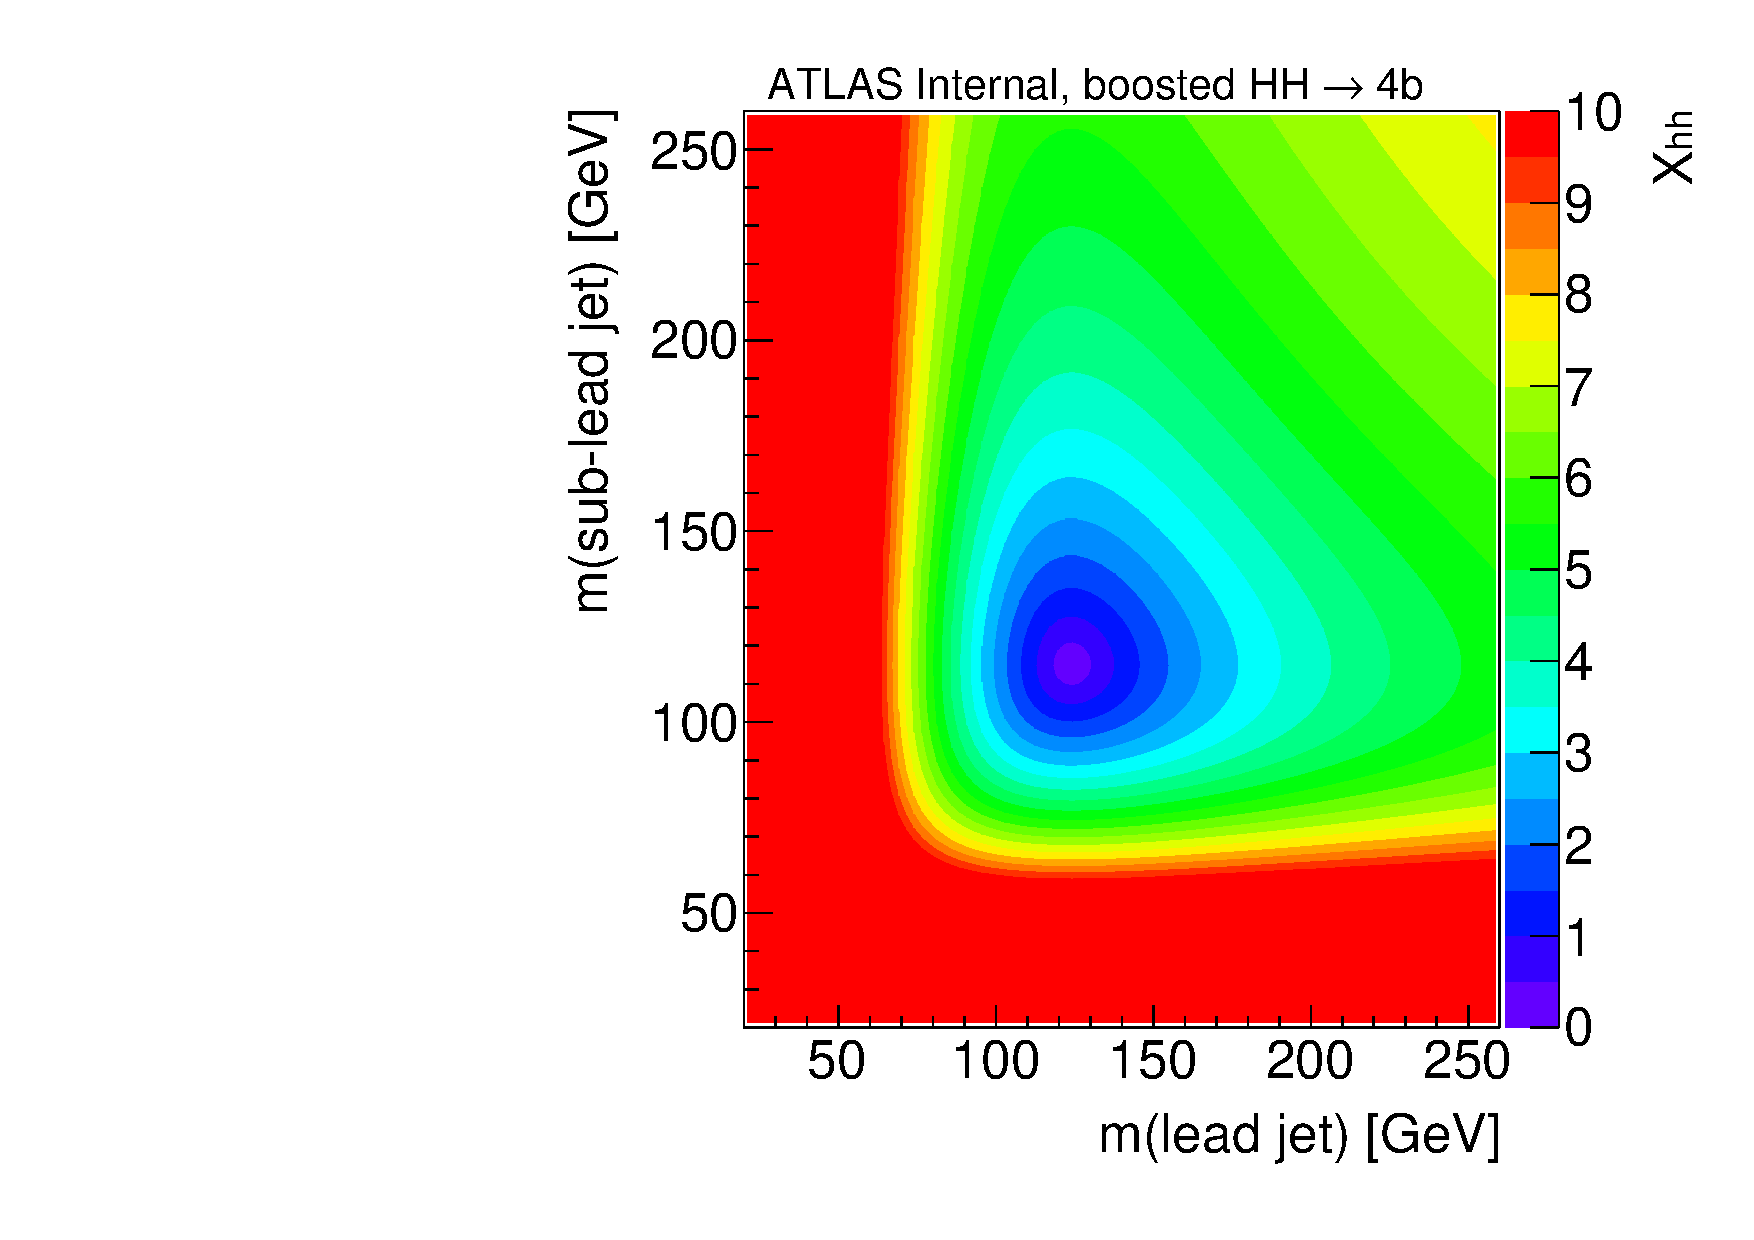
\includegraphics[width=0.45\textwidth,angle=-90]{figures/boosted/Other/cartoon-xhh.pdf}
  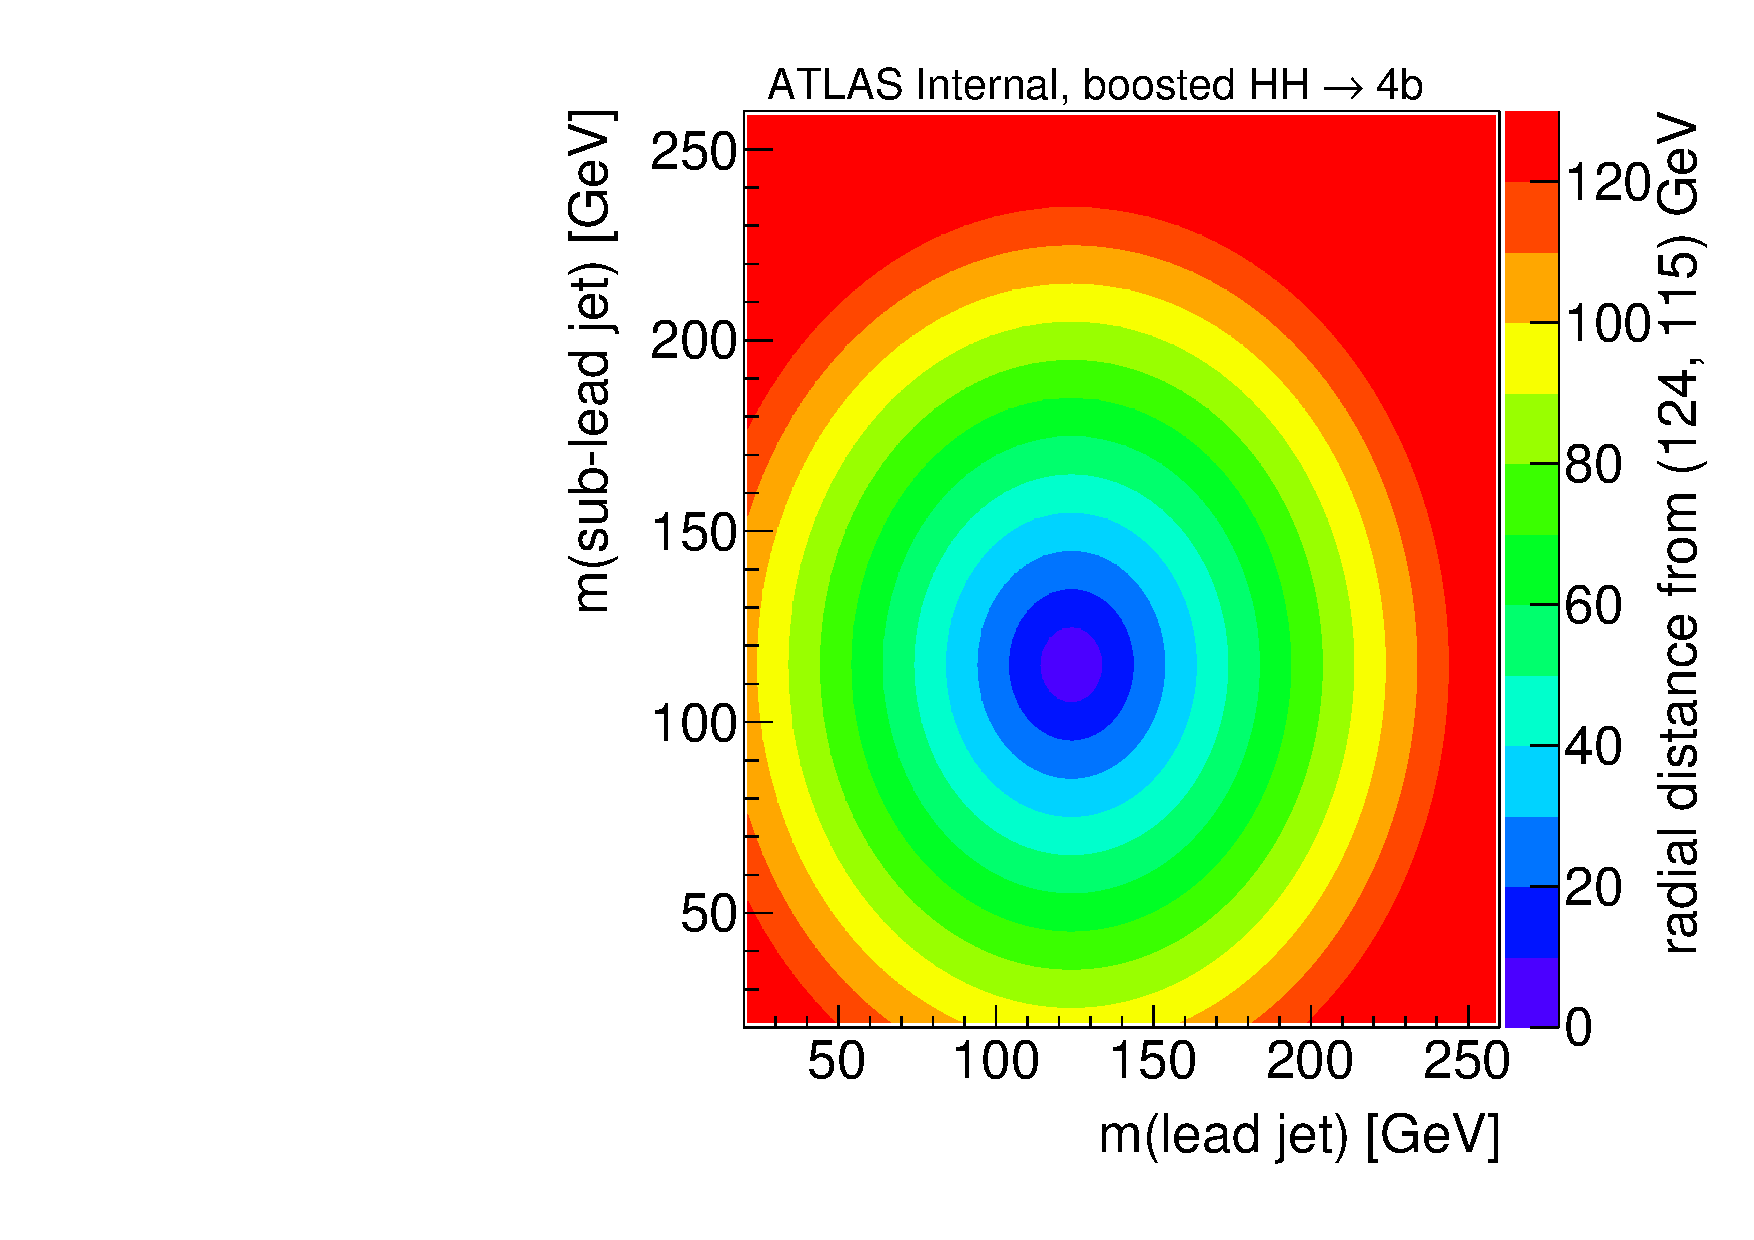
\includegraphics[width=0.45\textwidth,angle=-90]{figures/boosted/Other/cartoon-rhh.pdf}
  \caption{Values of the $X_{hh}$ and $R_{hh}$ variables, which are shapes in the two-dimensional plane of the large-R jet masses used to defined signal, control, and sideband regions. For both variables, a smaller value indicates the jets are closer to the Higgs mass. }
  \label{fig:boosted-regiondef-cartoons}
\end{center}
\end{figure}

The number of events in the control region and sideband region as a function of Resonance mass is shown in Figure~\ref{fig:boosted-selection-region-efficiency}. For 2$b$s, 3$b$ and 4$b$, each region has the number of events decrease from signal region to control region to sideband regions.

\begin{figure*}
\begin{center}
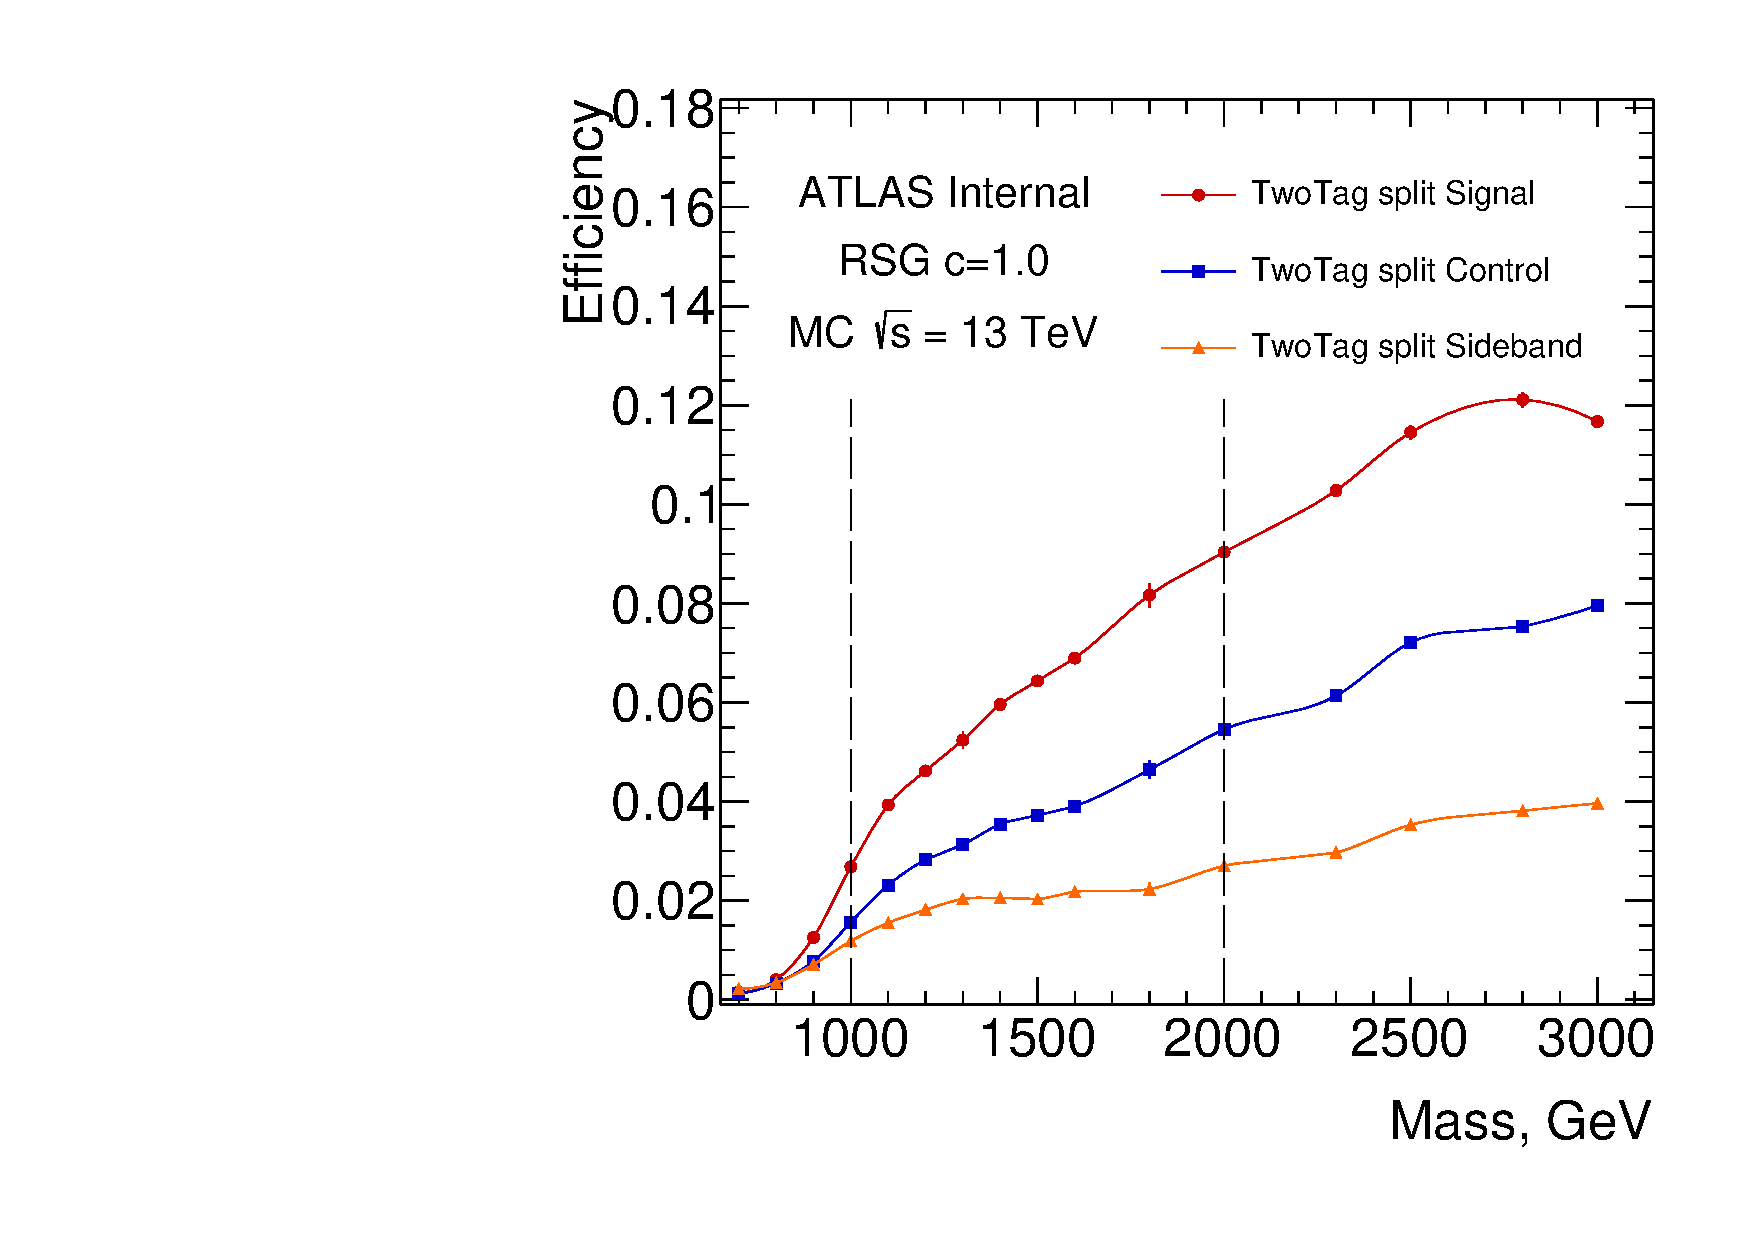
\includegraphics[width=0.48\textwidth,angle=-90]{figures/boosted/SigEff/region_2b_lst_Moriond_Efficiency_PreSel.pdf}
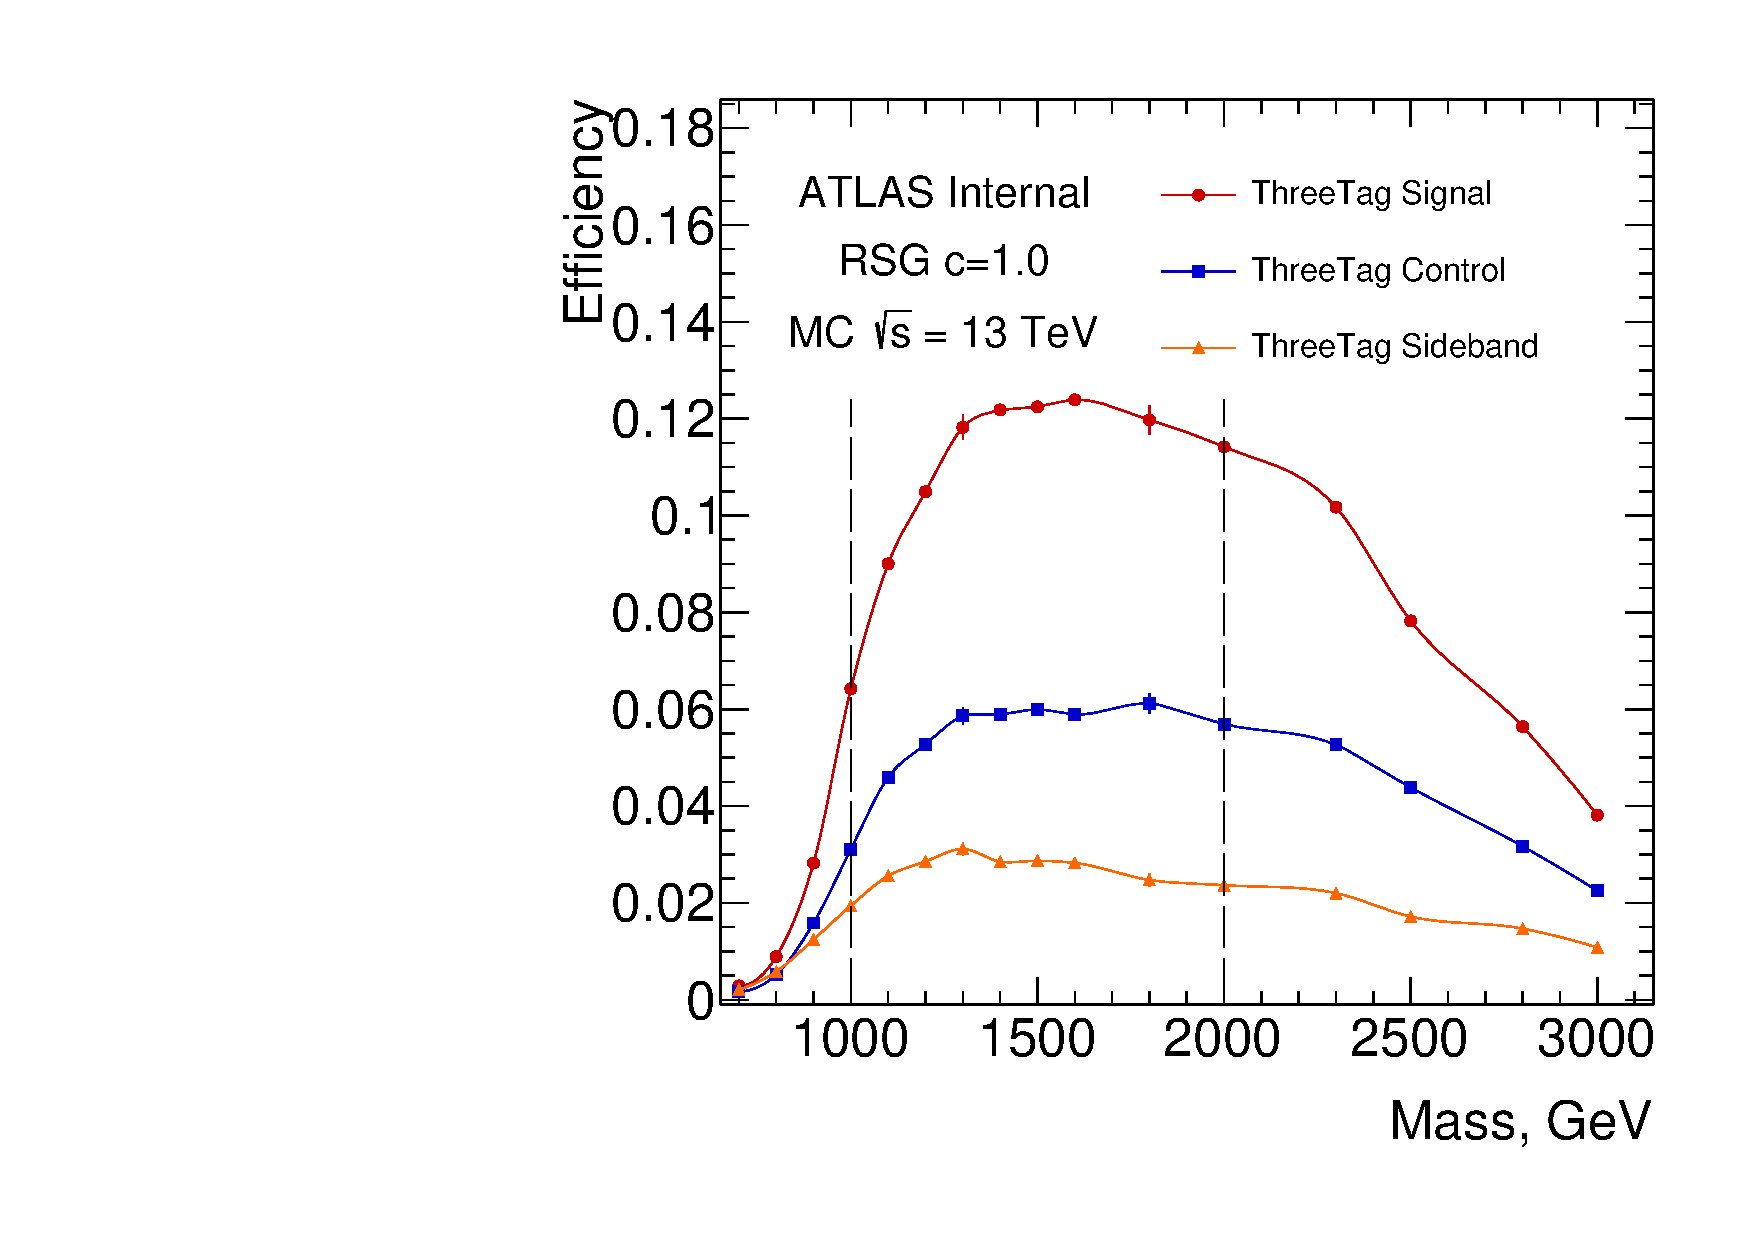
\includegraphics[width=0.48\textwidth,angle=-90]{figures/boosted/SigEff/region_3b_lst_Moriond_Efficiency_PreSel.pdf} \\
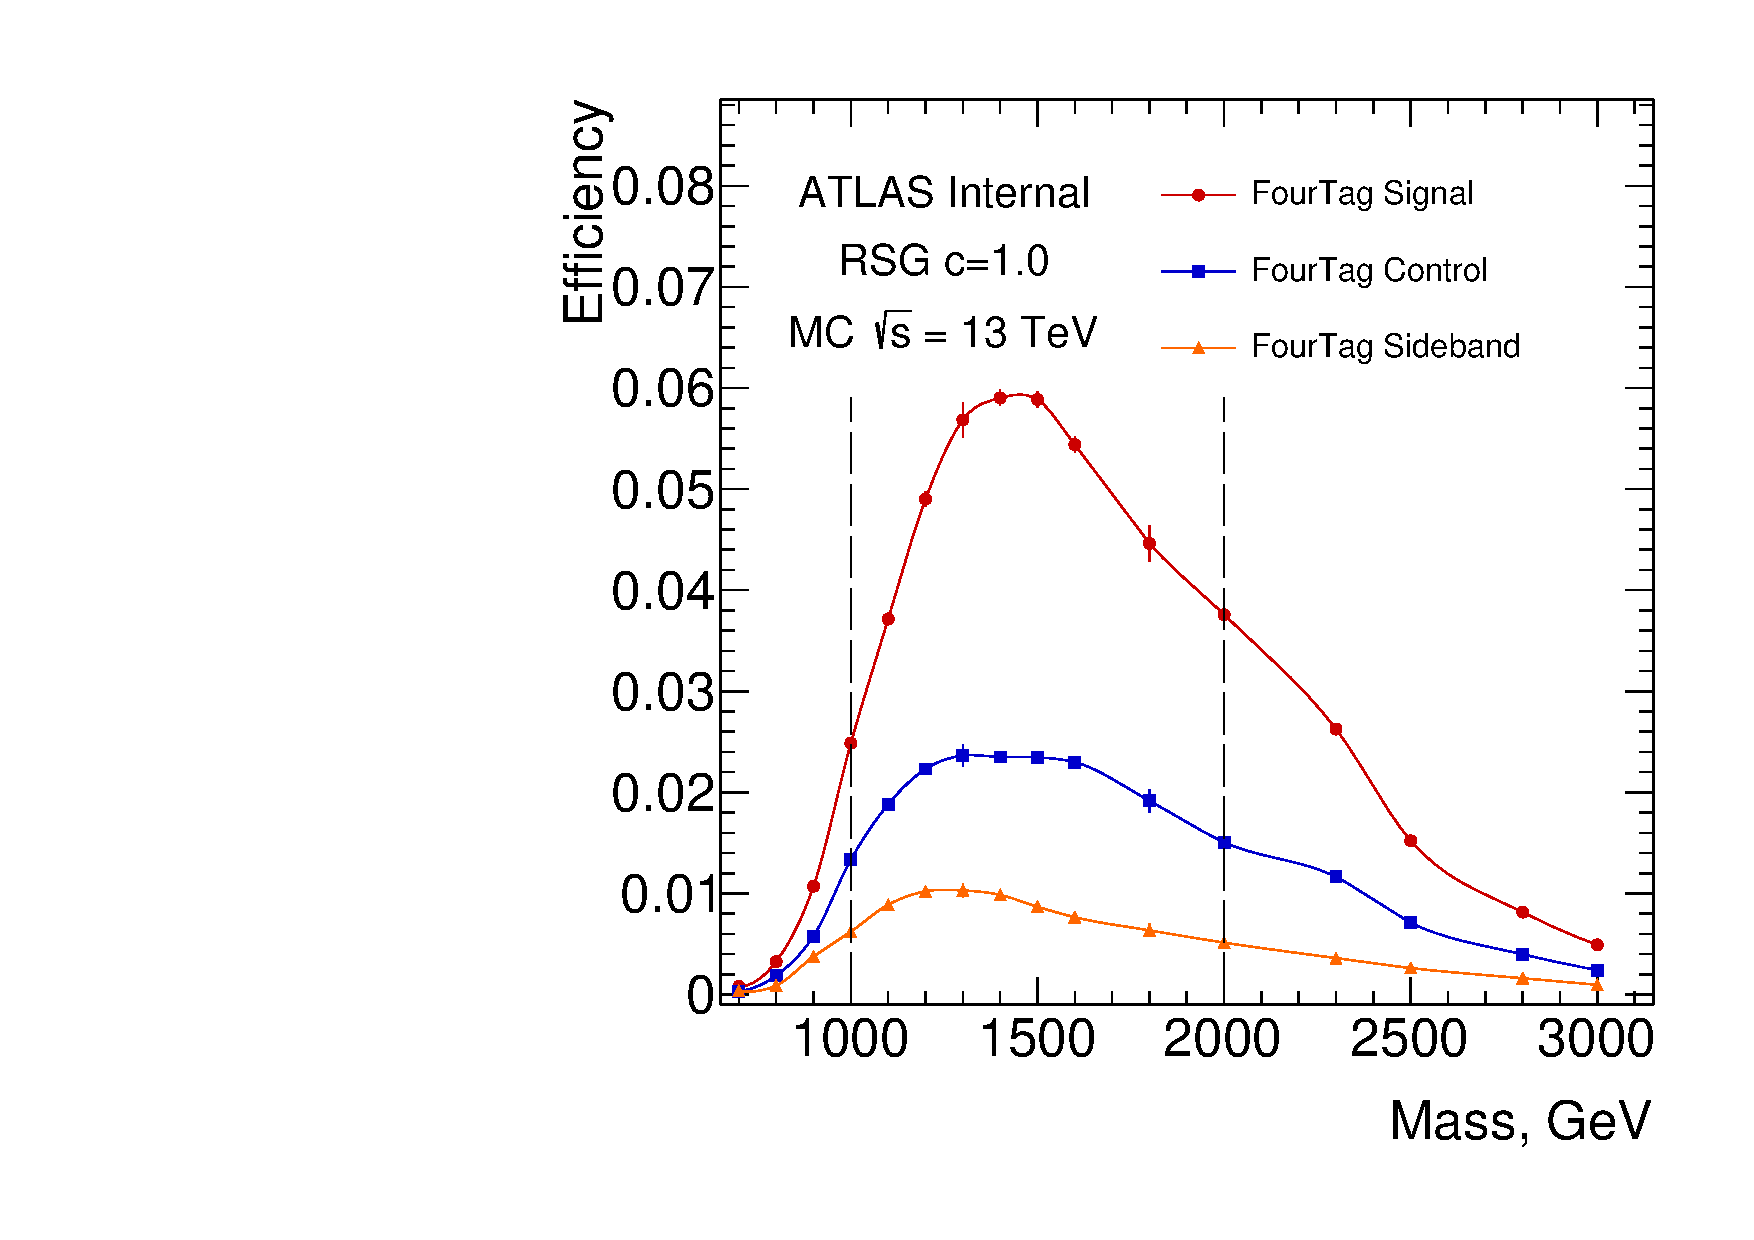
\includegraphics[width=0.48\textwidth,angle=-90]{figures/boosted/SigEff/region_4b_lst_Moriond_Efficiency_PreSel.pdf}
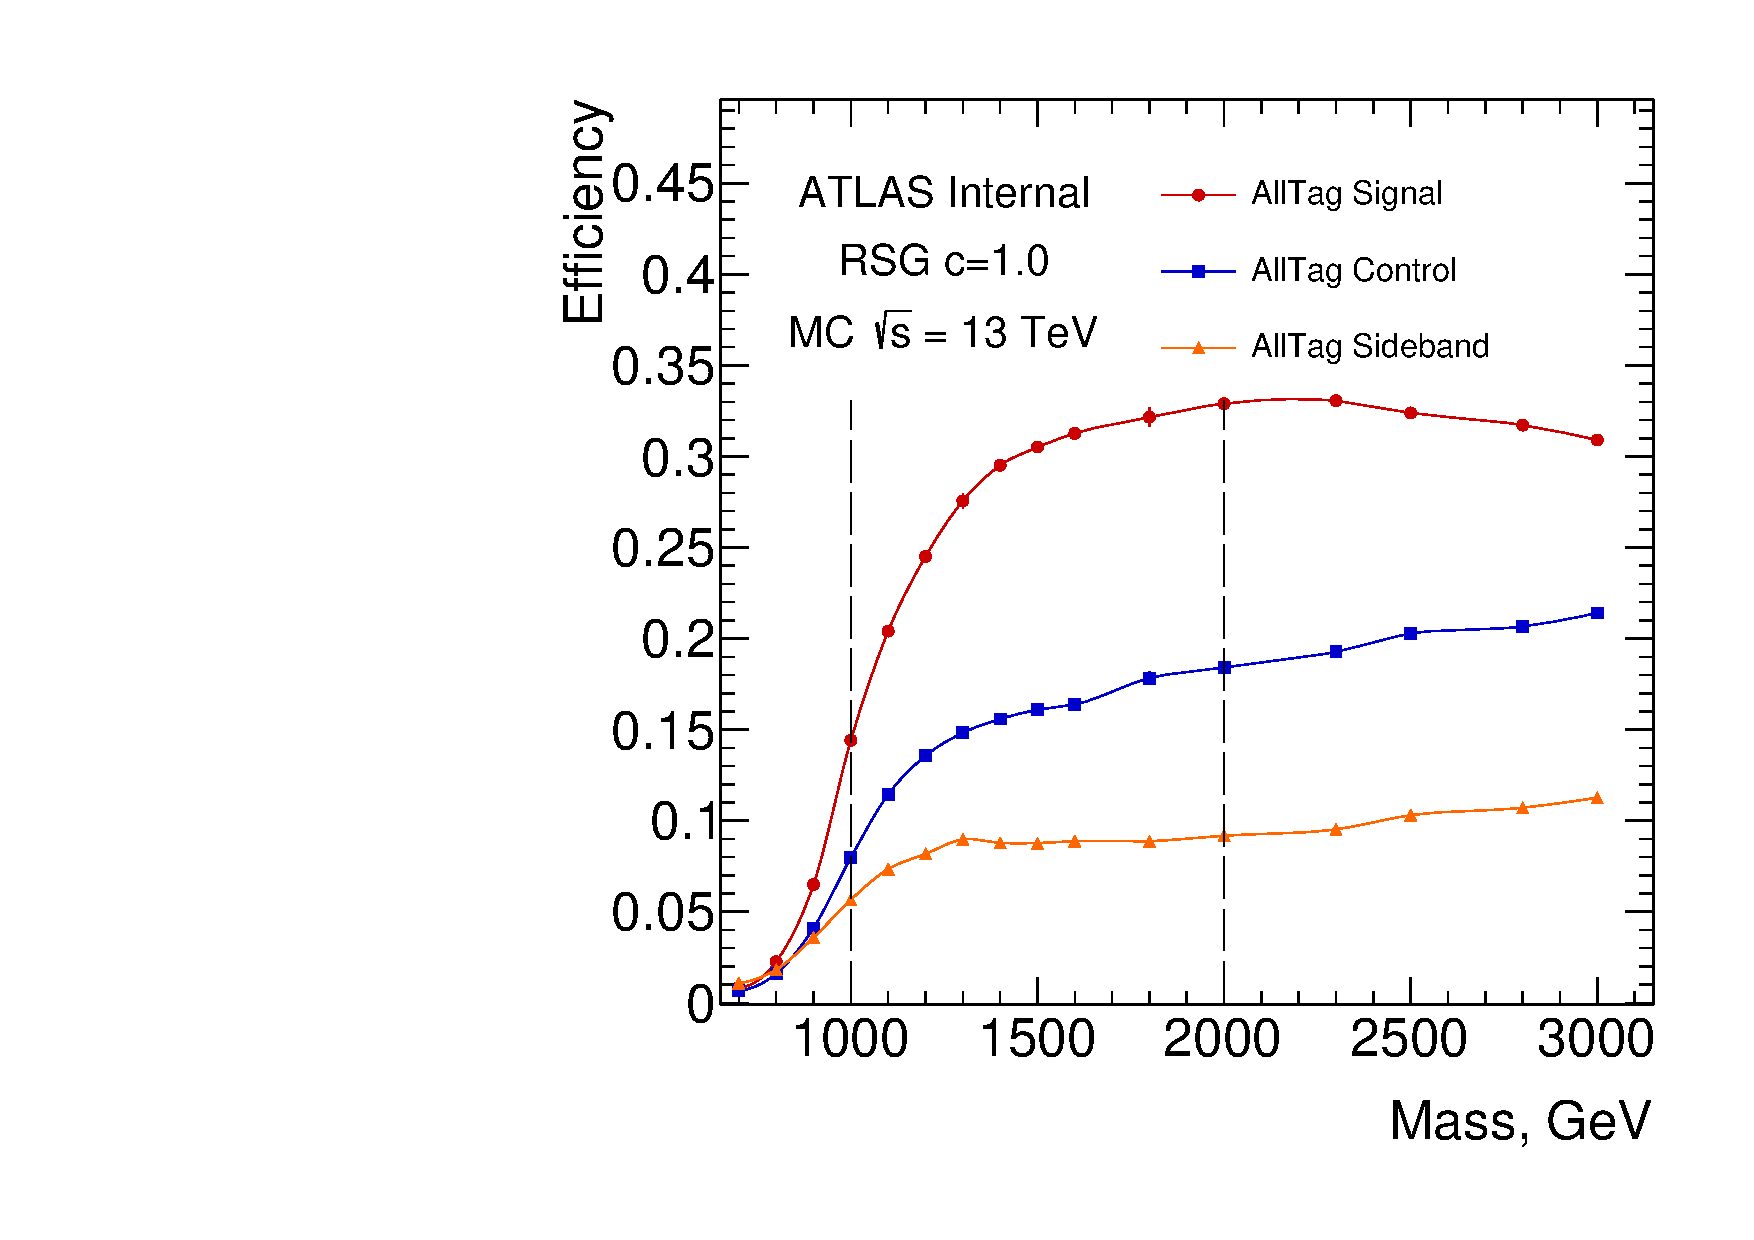
\includegraphics[width=0.48\textwidth,angle=-90]{figures/boosted/SigEff/region_alltag_lst_Moriond_Efficiency_PreSel.pdf} \\
  \caption{Detailed signal efficiency in different signal/control/sideband regions as in 2$b$s (top left, 3$b$ (top right), 4$b$ (bottom left) and inclusive b-tagged regions, which incluse 2$b$, 1$b$ and 0$b$ as well, (bottom right) as a function of signal resonance mass hypothesis for selection cuts. The efficiencies are relative to the total number of events in the preselection.}
  \label{fig:boosted-selection-region-efficiency}
\end{center}
\end{figure*}


%updated June 6 2017

\subsection{Overview}

\paragraph{}
The primary backgrounds to this analysis in the four $b$-jet signal region, in order of size, are QCD multi-jet production ($\sim 95\%$), $t\bar{t}$ ($\sim 5\%$), and $Z$+jets ($< 1\%$), where the percentages are the expected fraction of the background coming from each source. In the three $b$-jet signal region, the fractions are QCD ($\sim 90\%$), $t\bar{t}$ ($\sim 10\%$), and $Z$+jets ($< 1\%$).  In the two $b$-jet split signal region, the fractions are QCD ($\sim 80\%$), $t\bar{t}$ ($\sim 20\%$), and $Z$+jets ($< 1\%$).

\paragraph{}
QCD is by far the dominant background. However, there is no reliable, high-statistics Monte Carlo simulation sample in this region of phase space (i.e with three or four $b$-jets collected into two high-$p_{T}$ large radius jets) and thus a data-driven background estimation is needed. (See Appendix ~\ref{app:muqcd-study}.) For the \ttbar background, Monte Carlo simulation samples of reasonable size are available, and thus can be used to guide an estimation of this background. The $Z$+jets background is small enough that we will rely on the Monte Carlo simulation of $Z$+heavy flavor jets. $ZZ\to b\bar{b}b\bar{b}$ has been estimated to be completely negligible using a particle-level analysis, with less than one event expected after three $b$-tags are required, which will be further heavily suppressed by the $X_{hh}$ requirement.

\paragraph{}
The QCD background prediction relies on finding a region which is similar enough in event properties that it can be used to estimate the shapes of the expected QCD background.  This region is identical to the signal region defined by the full selection, with the exception that the events must have \textbf{less} $b$-tagged track jets:
\begin{itemize}
\item For the 2$b$s category, the 1$b$ sample is used for modeling.
\item For the 3$b$ and 4$b$ categories, the 2$b$ sample - where the two $b$-tagged trackjet are in the same large-$R$ jet - is used for modeling.
\end{itemize}
To prevent differences in the number of track jets from biasing the dijet mass distribution, the $1b$-tagged region requires that each large-$R$ jet has at least one track jet (to model $2bs$, ie. 2$b$ tag split). Similarly, the $2b$-tagged region requires that one large-$R$ jet has at least one track jet and the other one has at least two track jets (to model $3b$), and each large-$R$ jet has at least two track jets (to model $4b$).

\paragraph{}
However, this less $b$-tagged region only supplies the shapes of the expected background and not the total yield, and a second control sample, which we denote the \textit{Sideband} region, is used to estimate the yield. The Sideband is obtained by doing the full analysis selection, except instead of the $X_{hh}$ cut an alternative criteria on the large radius jet masses is used, that $33 < R_{hh} $ and $R_{hh}^{\text{high}} < 58$~\GeV. To validate this approach, a third region, which we denote the \textit{Control} region, is centered on the signal region in the plane of the two large radius jet masses but does not include the signal region, such that $R_{hh} < 33$~\GeV.  The control region is used to validate the background estimations before unblinding. The control and sideband regions are optimized, as shown in the following sections, to accurately estimate the rate of the QCD background (and thus allow for an extrapolation from the $1b$/$2b$ estimate to a prediction in the $4b/3b/2bs$  signal regions), whilst giving a control region which has kinematic properties similar to that of the signal region. 







\paragraph{}
The $t\bar{t}$ background shape is taken from MC. A data-based estimation of the $t\bar{t}$ background yield is performed simultaneously with the QCD background yield estimation, by means of a binned likelihood fit.
In the plane of the two leading large radius jet masses, the main contribution of the $t\bar{t}$ background lies in the Sideband region. The data distribution in the Sideband region of the leading-$p_{T}$ large radius jet mass is fit simultaneously with the QCD shape estimate (from the less $b$-tagged sample) and with the $t\bar{t}$ Monte Carlo shape. This fit is done separately in the 4$b$, 3$b$, and 2$b$s Sideband regions.
From this fit, two terms are determined simultanously: $\mu_{QCD}$ and $\alpha_{tt}$. $\mu_{QCD}$ is the ratio of the QCD event yield in the 2bs/3b/4b regions to the amount in each corresponding less b-tagged region. $\alpha_{tt}$ is the ratio of the fitted ttbar event yield to the yield predicted from ttbar MC.
These two numbers are then used as multiplicative constants in other regions of the mass plane (i.e. the Control or Signal regions) to extrapolate from the rates of the less $b$-tagged regions to predictions of rates in the 2bs/3/4 $b$-tagged regions, for estimating the amount of QCD, and to correct the rate of $t\bar{t}$ production wrt. MC. Hence, the underlying assumption is that these scale factors are roughly constant over the 2D large-R jet mass plane for Sideband/Control/Signal regions, which has been verified by perfoming these fits in small bins across the 2D mass plane. This is shown in Appendix ~\ref{app:muqcd-study}. The correction factors are derived separately for the 4$b$, 3$b$, and 2$b$s regions.

\paragraph{}
In this section, we describe this approach in more detail and show its validation in data.


\subsection{Definition of the sideband and control regions (SB, CR)}
\label{sec:boosted-SBCR}

\paragraph{}

The definitions of the SB, CR, and SR in the leading ($m^{\rm lead}_{\rm J}$) and sub-leading ($m^{\rm subl}_{\rm J}$) large-$R$ jet mass plane are found in Table~\ref{tab:boosted-sbcr-constraints}. These regions can be seen in the leading and sub-leading large-$R$ jet mass plane in Figure~\ref{fig:boosted-region-def}. As a reminder, the definition of $X_{hh}$, $R_{hh} $ and $R_{hh}^{\text{high}}$ are:

\begin{equation}
X_{hh} = \sqrt{\left(\frac{m^{\rm lead}_{\rm J} - \text{124 GeV}}{\sigma\left(m^{\rm lead}_{\rm J}\right)}\right)^2 + \left(\frac{m^{\rm subl}_{\rm J}-  \text{115 GeV}}{\sigma\left(m^{\rm subl}_{\rm J}\right)}\right)^2}, \\
R_{hh} = \sqrt{ (m^{\rm lead}_{\rm J} - 124)^2 + (m^{\rm subl}_{\rm J} - 115)^2 }, \\
R_{hh}^{\text{high}} = \sqrt{ (m^{\rm lead}_{\rm J} - 134)^2 + (m^{\rm subl}_{\rm J} - 125)^2 }.
\end{equation}

\begin{table}[htbp!]
\begin{center}
\begin{tabular}{c|c}
\hline
  Region                                      & Definition \\
  \hline
  Signal Region (SR) & $X_{hh}$ < 1.6\\
  Control Region (CR) & $R_{hh}$ < 33~\GeV\ and $X_{hh}$ > 1.6 \\
  Sideband Region (SB) & 33~\GeV < $R_{hh}$ and $R_{hh}^{\text{high}}$ < 58~\GeV
  \end{tabular}
\caption{Definitions of the Signal (SR), Sideband  (SB) and Control (CR) regions.}
\label{tab:boosted-sbcr-constraints}
\end{center}
\end{table}

\begin{figure*}[htbp!]
\begin{center}
  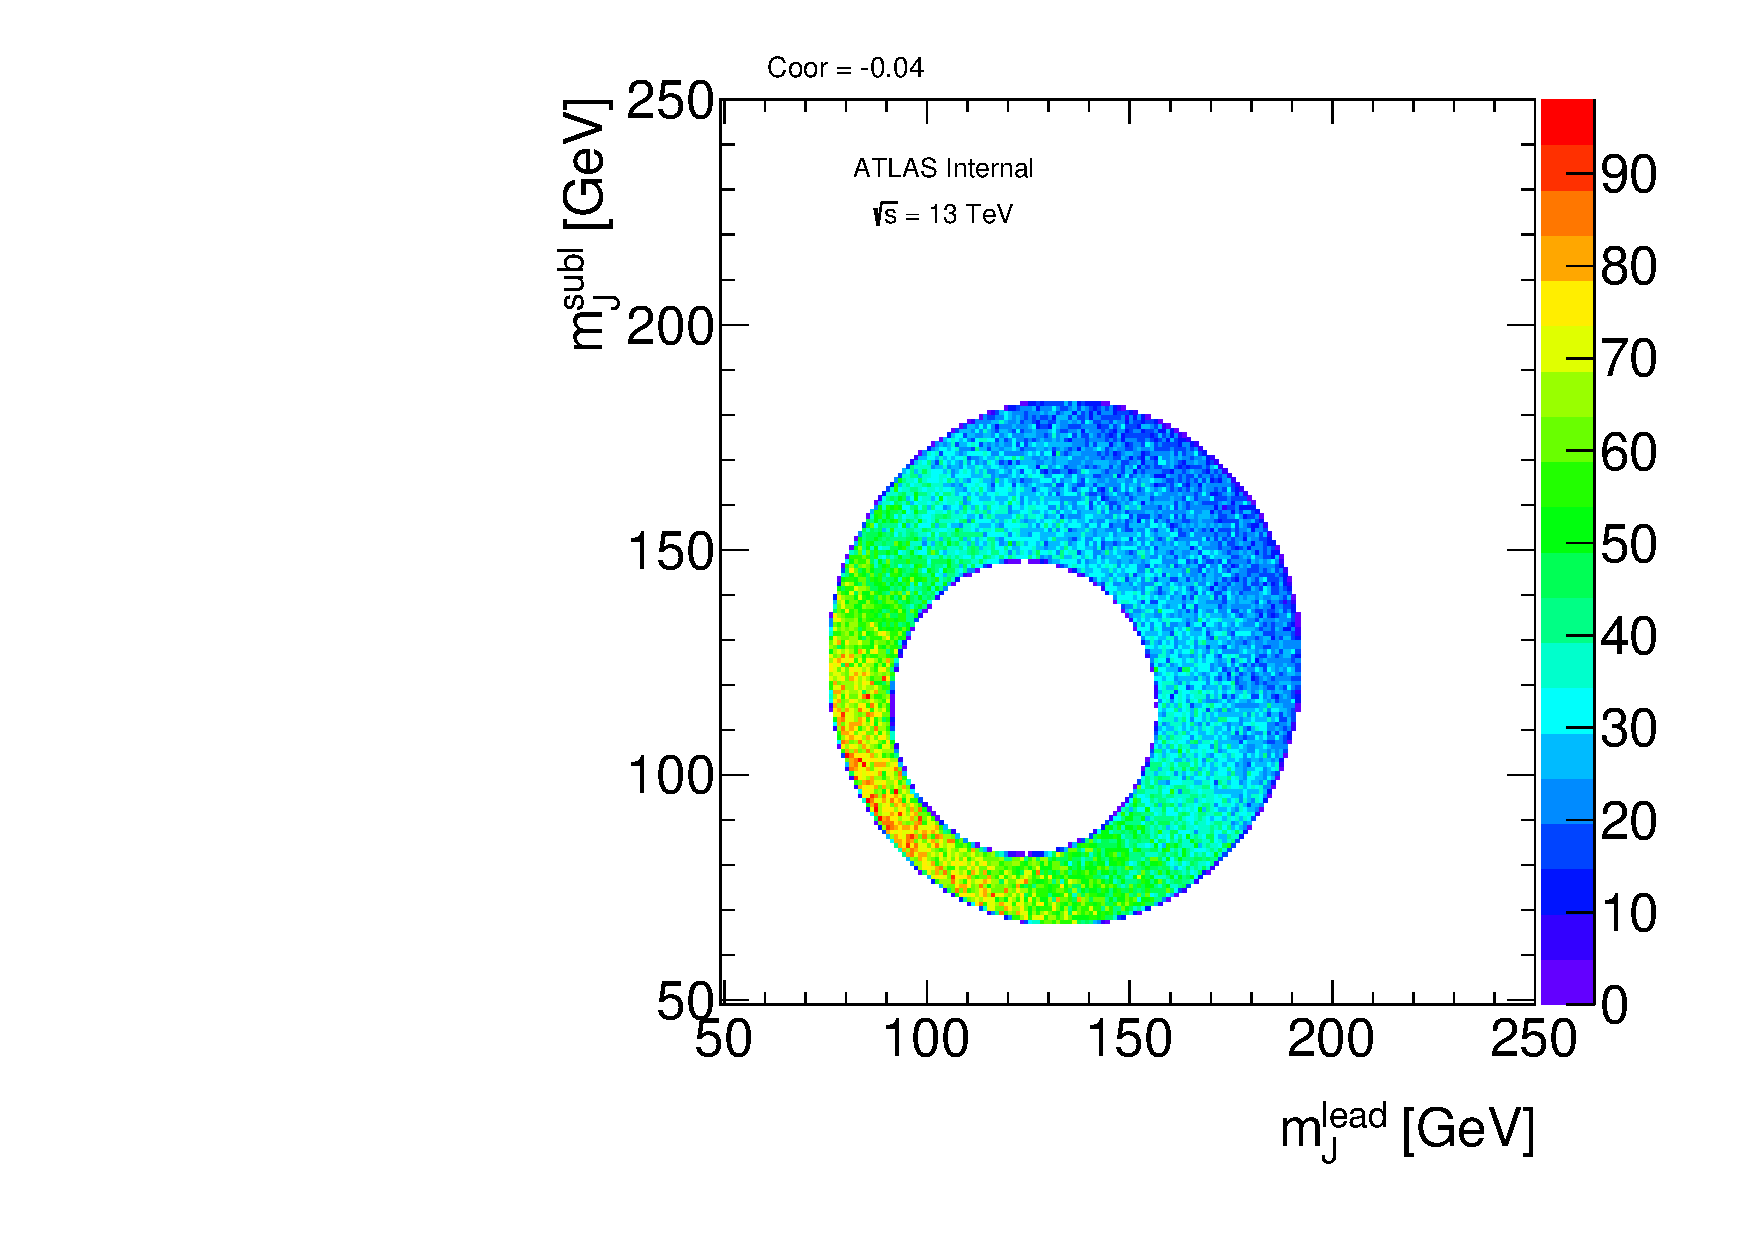
\includegraphics[angle=270, width=0.45\textwidth]{./figures/boosted/Other/Sideband_OneTag_mH0H1.pdf}
  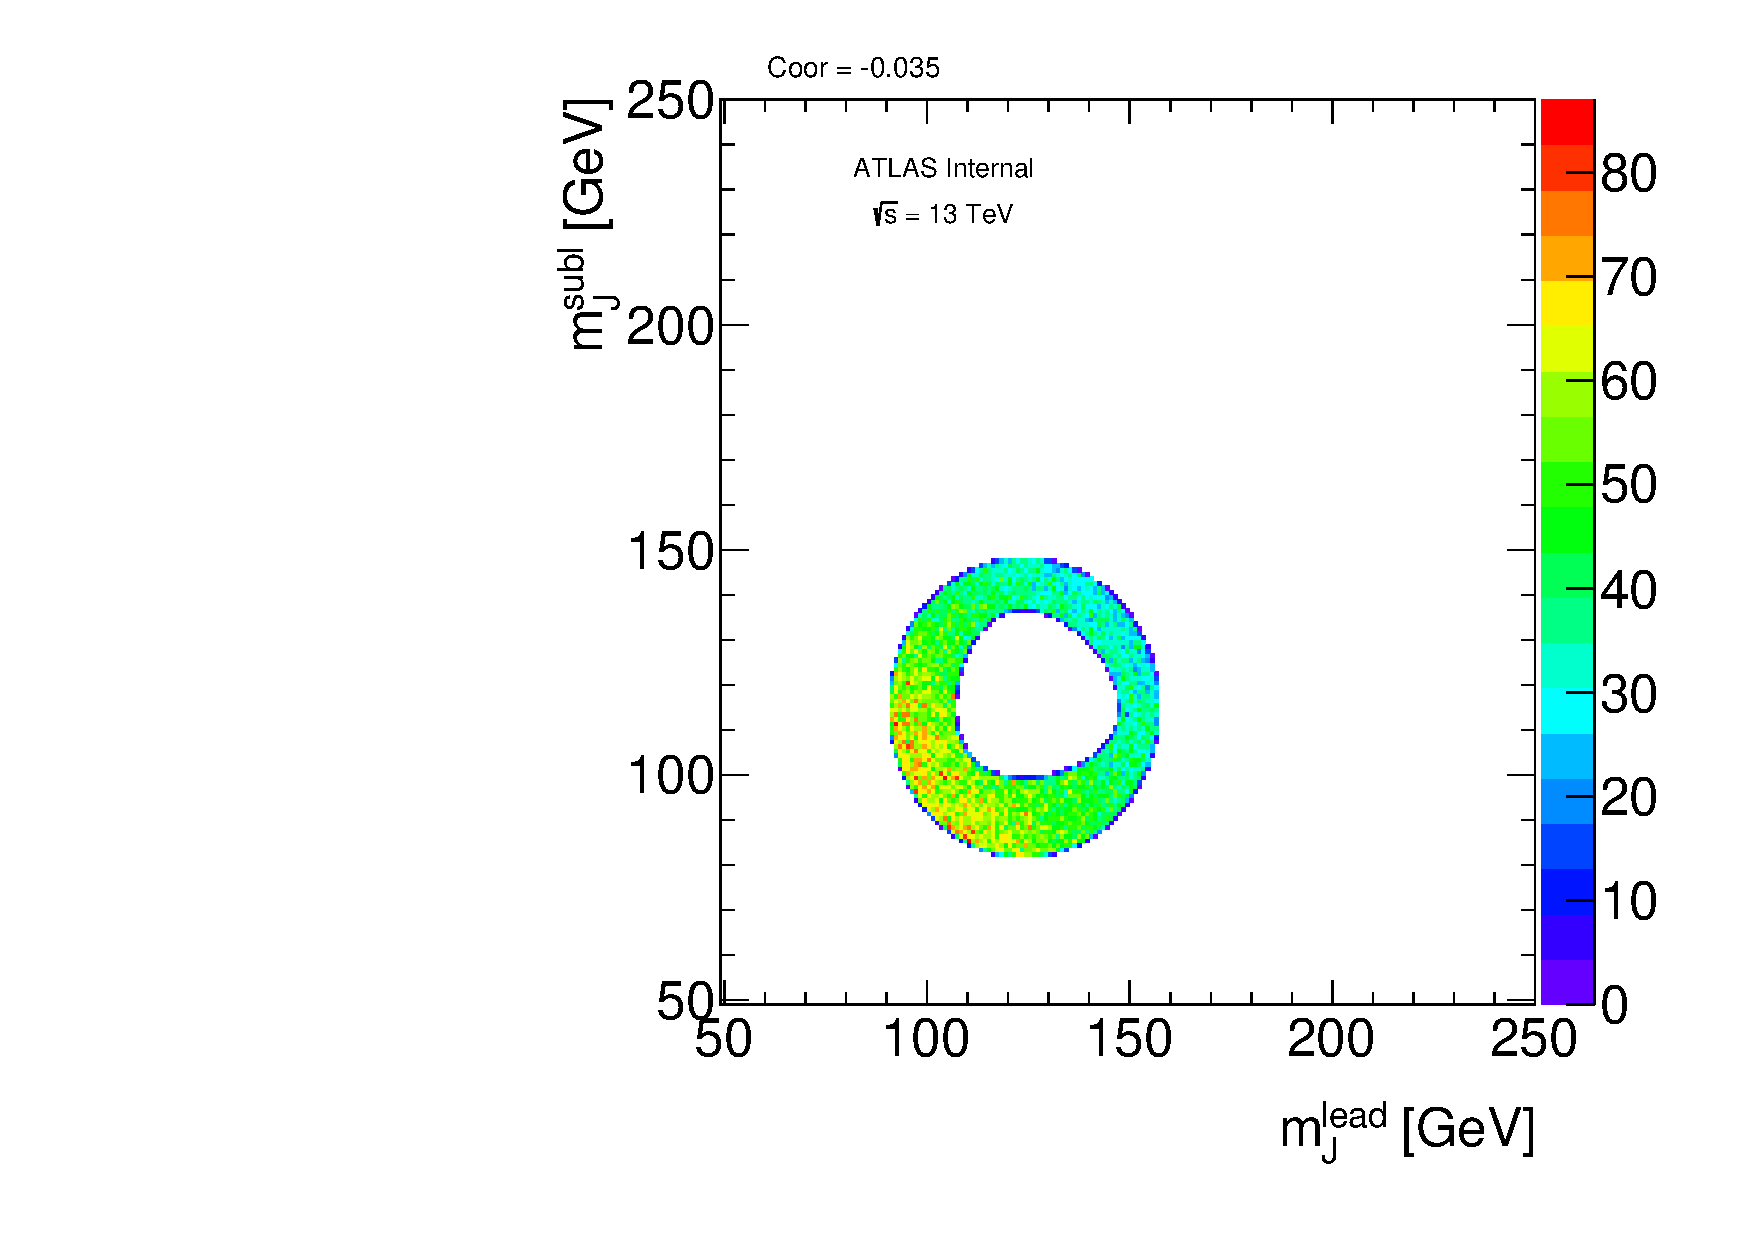
\includegraphics[angle=270, width=0.45\textwidth]{./figures/boosted/Other/Control_OneTag_mH0H1.pdf}\\
  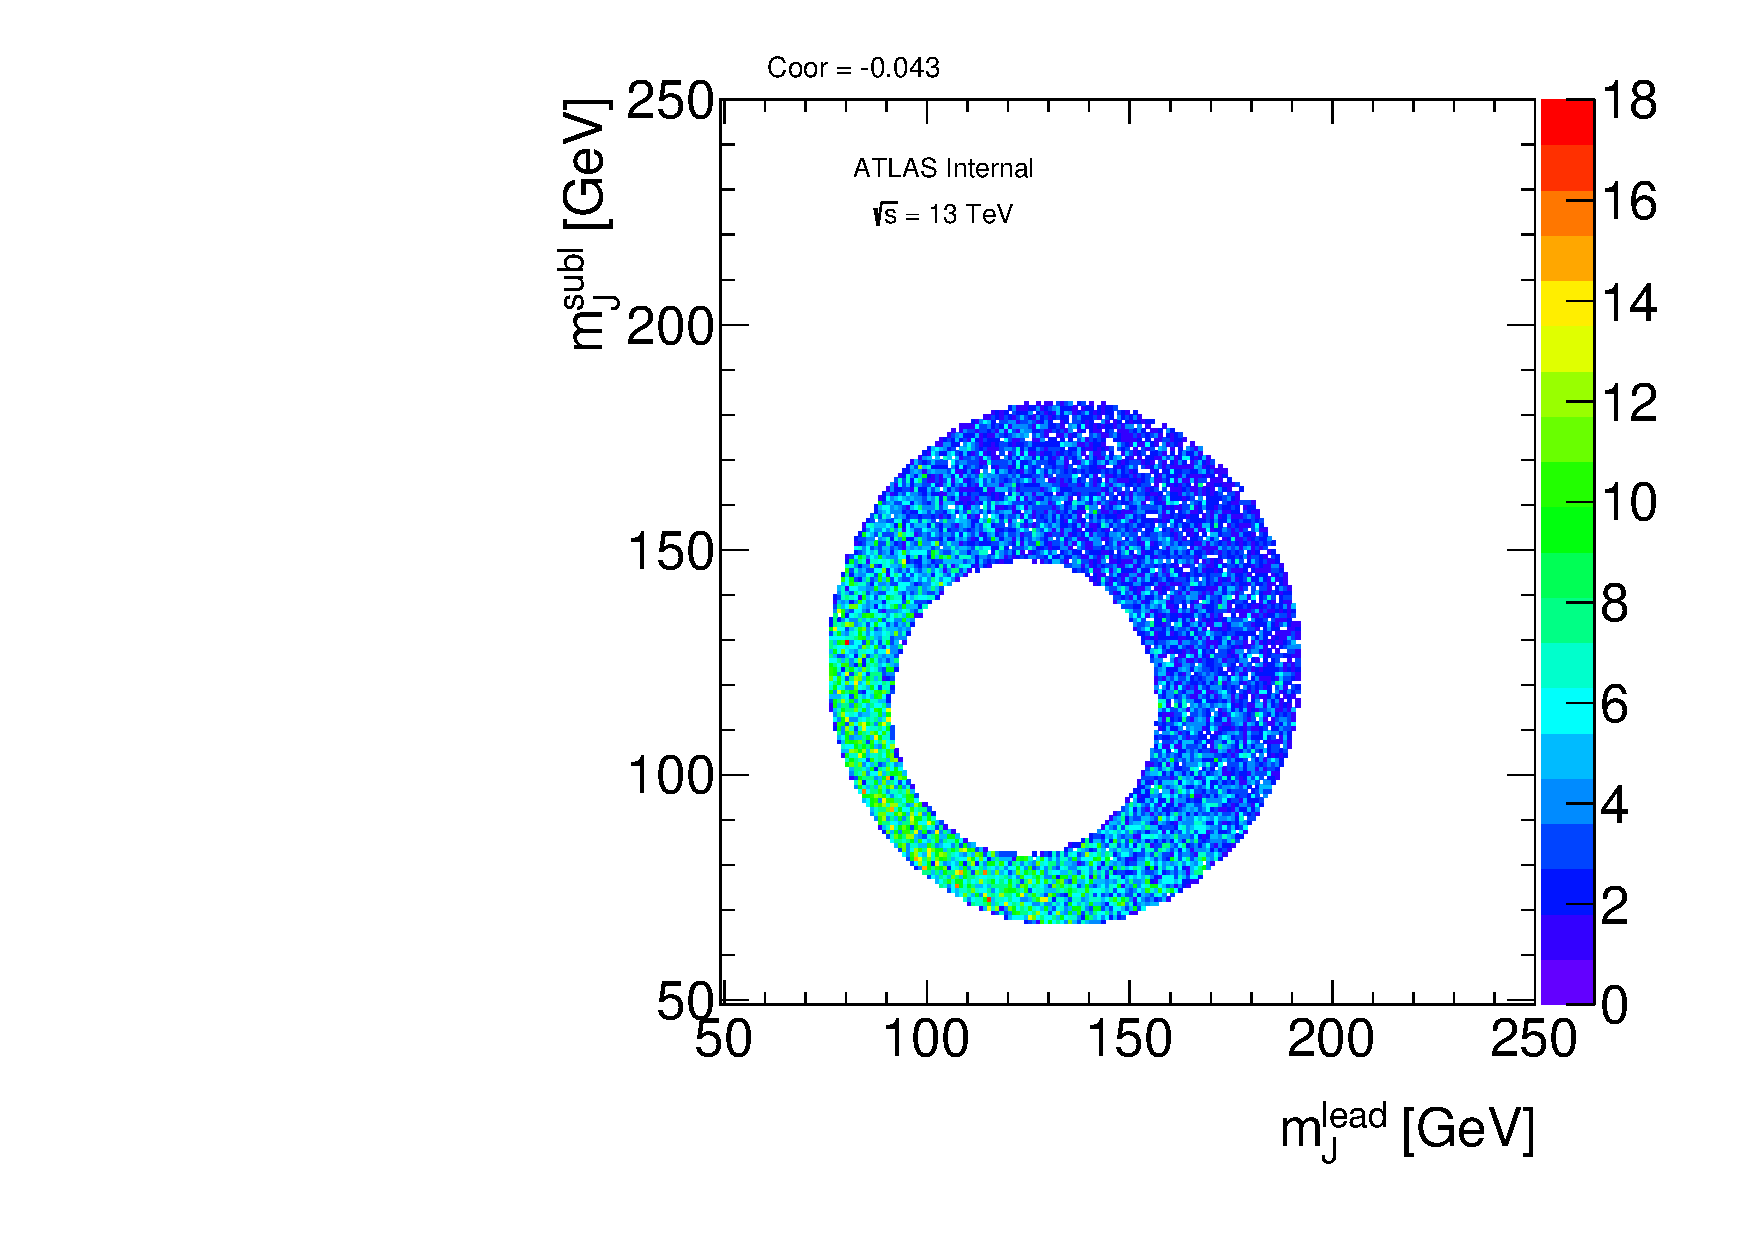
\includegraphics[angle=270, width=0.45\textwidth]{./figures/boosted/Other/Sideband_TwoTag_mH0H1.pdf}
  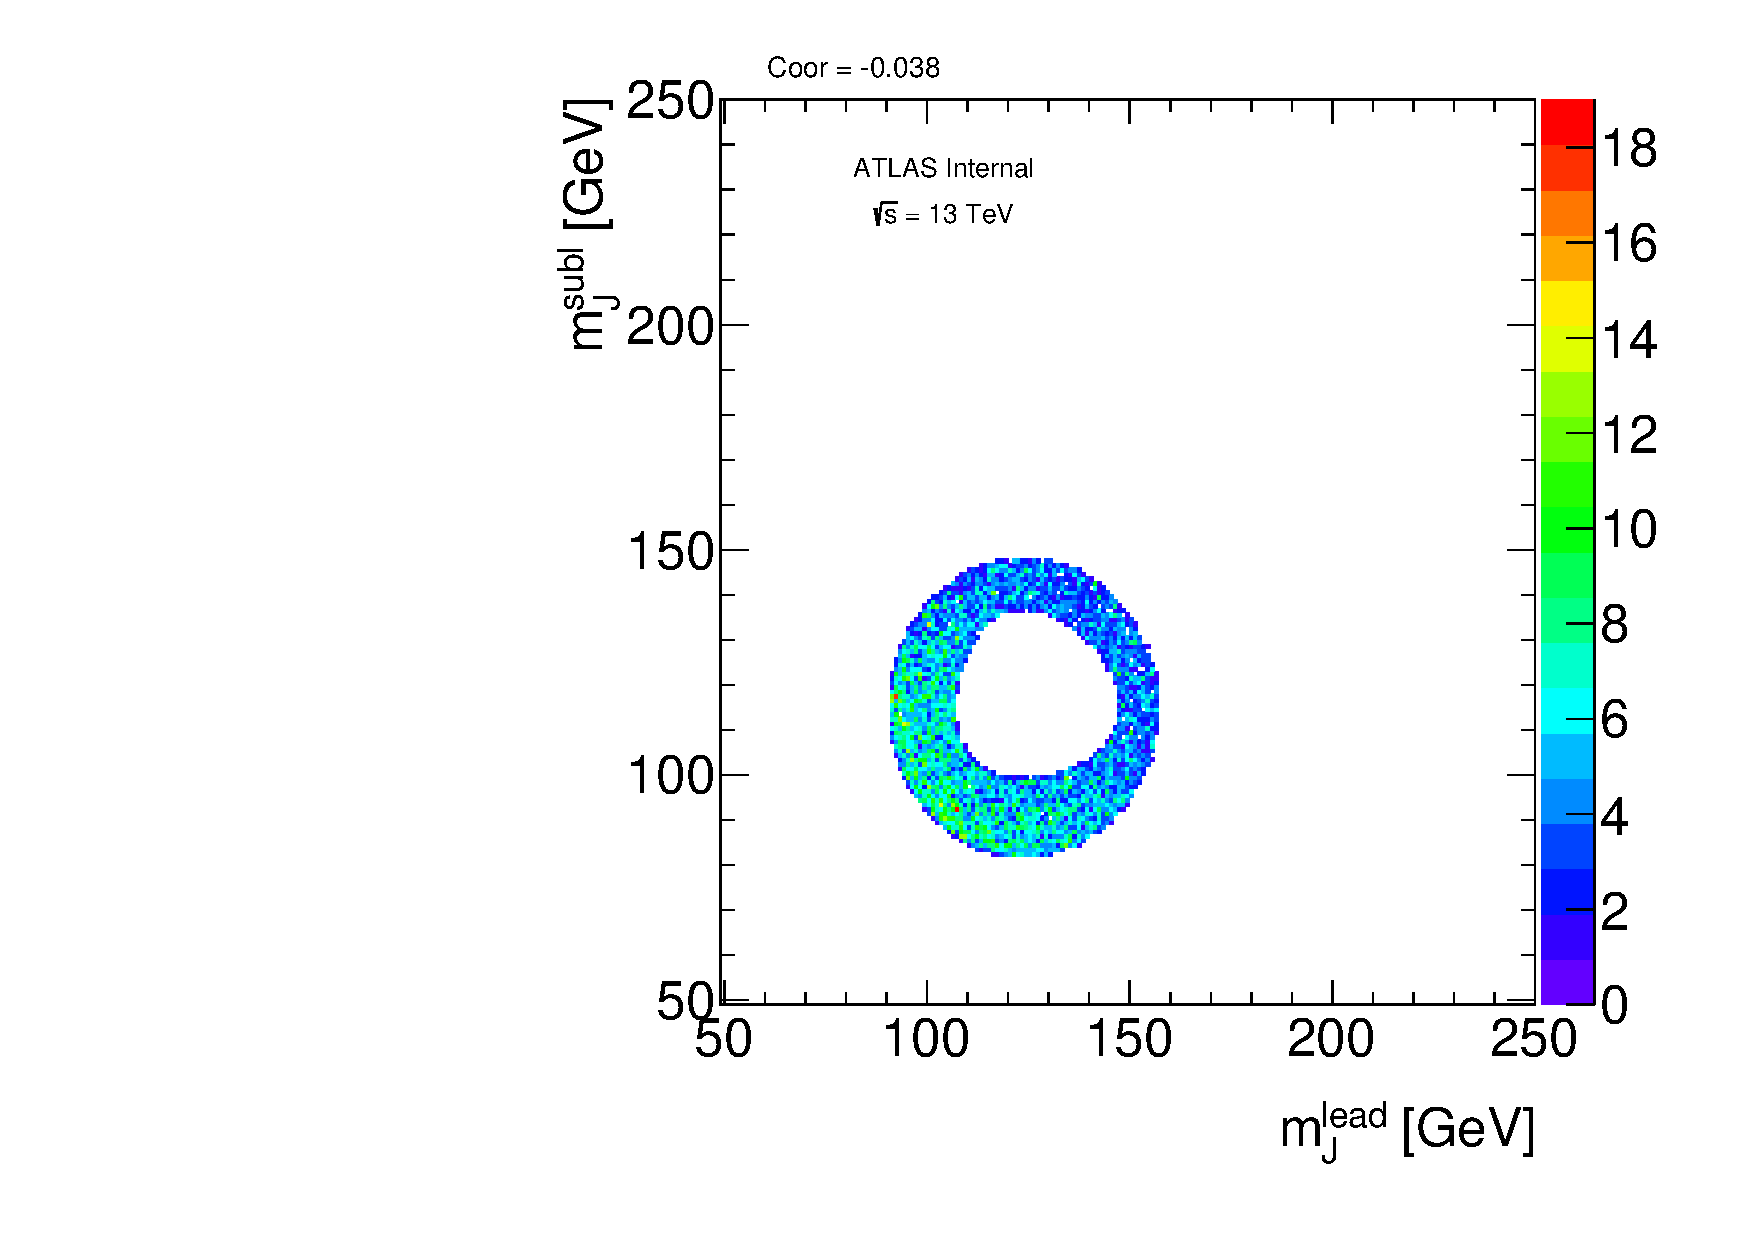
\includegraphics[angle=270, width=0.45\textwidth]{./figures/boosted/Other/Control_TwoTag_mH0H1.pdf}
  \caption{$m_J^{lead}$ vs. $m_J^{subl}$ in data in the 1$b$-tag (top) and 2$b$-tag (bottom) selection, the plots show the boundary between the Sideband (left) and Control (right) regions.}
  \label{fig:boosted-region-def}
\end{center}
\end{figure*}

\paragraph{}
The CR is chosen to be as close as possible to the signal region, thus allows a good test for the background predictions, avoids the top mass peak around 175 GeV, and still gives reasonably statistics.  The SB definition is optimized so as to also be a reasonable proxy for the events contained in the CR and SR. Being farther from the SR means that the exact kinematics will not be the same, but one can avoid very large and very small mass jets not present in the SR by appropriate choice of SB.   The optimization of teh CR and SB definitiona can be found in Appendix~\ref{app:SB-optimization}. The choice of SB's impact on the predicted QCD background normalization, which is derived from the SB, can be found in Appendix~\ref{app:muqcd-study}.


\pagebreak{}
\subsection{QCD multi-jets}
\label{sec:boosted-qcd}

\paragraph{}
The QCD multi-jets prediction relies on finding a region which is similar enough in event properties so that it can be used to estimate the shapes of the expected background. This region is defined to be identical to the signal region except requiring both of the large-$R$ jets to pass the $\geq 2$( like in $4b$) or $\geq 1/2$ (like in $3b$) or $\geq 1$(like in $2b$ split) track jet requirement, but have two or one associated $b$-tagged track jets only on one of the large-$R$ jets. However, this $1b/2b$ region only provides shapes of the expected background and not the total yield. 

\paragraph{}
It should be noted that the $1b/2b$ region is orthogonal to the $4b/3b/2bs$ signal regions. In addition, the MC predicted $t\bar{t}$ events in the $1b/2b$ regions are subtracted from the data to produce the $1b/2b$ QCD estimation. This procedure follows closely the method used in Run 1 and also used in the resolved analysis, but requiring $1b$-tag for the $2bs$ background estimation.

\label{par:boosted-qcd-2bseperate}
\paragraph{} It should also be noted that the $2b$ sample is further split into $80\%-20\%$ parts, where each is used separately for 3$b$ and 4$b$ background estimations. This ensures the shape estimations of 3$b$ and 4$b$ QCD estimates are uncorrelated. 

It should also be noted that the resolved veto will impact the 4$b$ background estimation.  Specifically, 2$b$ events are excluded when they have at least two resolved jets that are $b$ tagged (passing resolved $70\%$ working point) and passing the resolved $Xhh < 1.6$ cut if using two other non b-tagged resolved jets to make the Higgs candidates. This ensures that a similar sculpting effect is reflected in the background estimation, and a check for this can be found in Appendix ~\ref{app:resveto}.

Given the $1b/2b$ samples, which predict shapes for the QCD background, the normalization of the QCD background is determined in the sideband by fitting the leading jet mass distribution simultaneously with QCD and $t\bar{t}$ background templates, as described in section~\ref{sec:ttbarnorm}.  This fit gives a scaling factor for QCD, called $\mu_{QCD}$ (and for $t\bar{t}$, called $\alpha_{t\bar{t}}$) which can be applied to scale the $1b/2b$ predictions in the CR or SR to the predicted normalizations in those regions.

It should be noted that there can be kinematic differences between the  $1b/2b$ samples and the $4b/3b/2bs$ regions.  Thus a kinematic reweighting is applied to correct for such differences, as described in Section~\ref{sec:boosted-reweight}.


%\paragraph{} 
%This background estimation is contingent on the idea that the 0$b$ sample QCD shape is a good estimate of $4/3/2bs$ samples QCD shapes. In addition, the use %of the SB region to estimate the background normalization relies on the SB to also accurately describe the normalization in the CR and SR regions.  The %purpose of the CR is thus to test both of these hypotheses. 

%\paragraph{} 
%While the normalizations of the $4b/3b/2bs$ split QCD predictions will be different, as they use events in the respective $4b$, $3b$, $2bs$ SB regions to set the normalizations, the shape estimates for the $4b/3b/2bs$  QCD predictions will be similar as they are both derived from the $1b/2b$ sample but only differ based on the number of $b$-tagged track jets required in each \largeR\ jet.



%As a final note, as discussed in Appendix~\ref{app:boosted_signal_migration}, we want to avoid possible signal contamination in the $2b$ regions used in our QCD predictions.  The primary concern for this contamination is in the SR prediction at high mass, where the expected backgrounds are small.  As such, in the $2b$ sample in the SR, we do not use (or look at) events above 2 TeV.  For background predictions above 2 TeV, we will perform a background smoothing up to 2 TeV using an exponential function, and will extrapolate above 2 TeV (see Section~\ref{sec:boosted-SR-smoothing}).  The choice of 2 TeV as a transition point was determined by ensuring that the signal contamination in dijet mass regions was at the few percent level or less (even when scaling by expected signal strength limits), as described in more detail in  Section~\ref{sec:boosted-SR-smoothing}.


%%%%%%%%%%%%%%%%%%%%%%%%%%%%%%%%%%%%%%%%%%%%%%%%%%%%%%%%%%%%%%%%%%%%%%%
%%%%%%%%%%%%%%%%%%%%%%%%%%%%%%%%%%%%%%%%%%%%%%%%%%%%%%%%%%%%%%%%%%%%%%%
%%%  SB. CR
%%%%%%%%%%%%%%%%%%%%%%%%%%%%%%%%%%%%%%%%%%%%%%%%%%%%%%%%%%%%%%%%%%%%%%%
%%%%%%%%%%%%%%%%%%%%%%%%%%%%%%%%%%%%%%%%%%%%%%%%%%%%%%%%%%%%%%%%%%%%%%%



\pagebreak{}
\subsection{\ttbar background}
\label{sec:boosted-ttbar}

\paragraph{}
The number of \ttbar\ events in the signal region coming mainly from the all-hadronic decay mode (with a smaller contribution from the leptonic + jets decay mode) comprises of  around 5-20\%  of the inclusive total background in the $4b/3b/2bs$ regions due to the high \pt\ threshold imposed on the leading \largeR calorimeter jet. In addition, the normalization and the shape of \ttbar\ events in the sideband region can affect the QCD estimate described in the previous section.

\paragraph{}
For the normalization of the $t\bar{t}$ background, we start with the MC prediction estimated by scaling the MC sample by the cross section and luminosity, and then applying the boosted event selection.  To account for possible differences between data and MC, a normalization scaling factor  is derived from a fit to data in the sideband region.  Although estimated in the SB, this normalization scaling factor will be applied also in the CR and SR.  Separate fits are done in the $4b/3b/2bs$  SB, thus deriving separate normalization scaling factor for the $4b/3b/2bs$ samples. For the shape of the $t\bar{t}$ background, no data driven methods were identified, and thus the MC shape is used.  

\paragraph{}
However, it should be noted that in the $4b$ and $3b$ signal region, there were not sufficient MC statistics to get a reasonable shape estimate.  As a result, in the $4b$ and $3b$ signal region,  the $2bs$ shapes will be used (but the normalization will still be that estimated for the $4b$/$3b$ sample). Since the same shape is used for the $4b/3b/2bs$ SR predictions of $t\bar{t}$, the shape systematics are considered correlated in the final results and limit setting. A comparison between the $4b/3b/2bs$ shapes for the di-large-$R$-jet mass distributions (the final discriminant) in the SR can be found in Figure~\ref{fig:ttshapeComp}.  As we can see, the shapes are compatible, with the $4b$ having much larger statistical uncertainties.  Differences between these distributions will be used as a systematic, as described in Section~\ref{sec:systematics}.

\begin{figure}[htbp!]
\begin{center}
  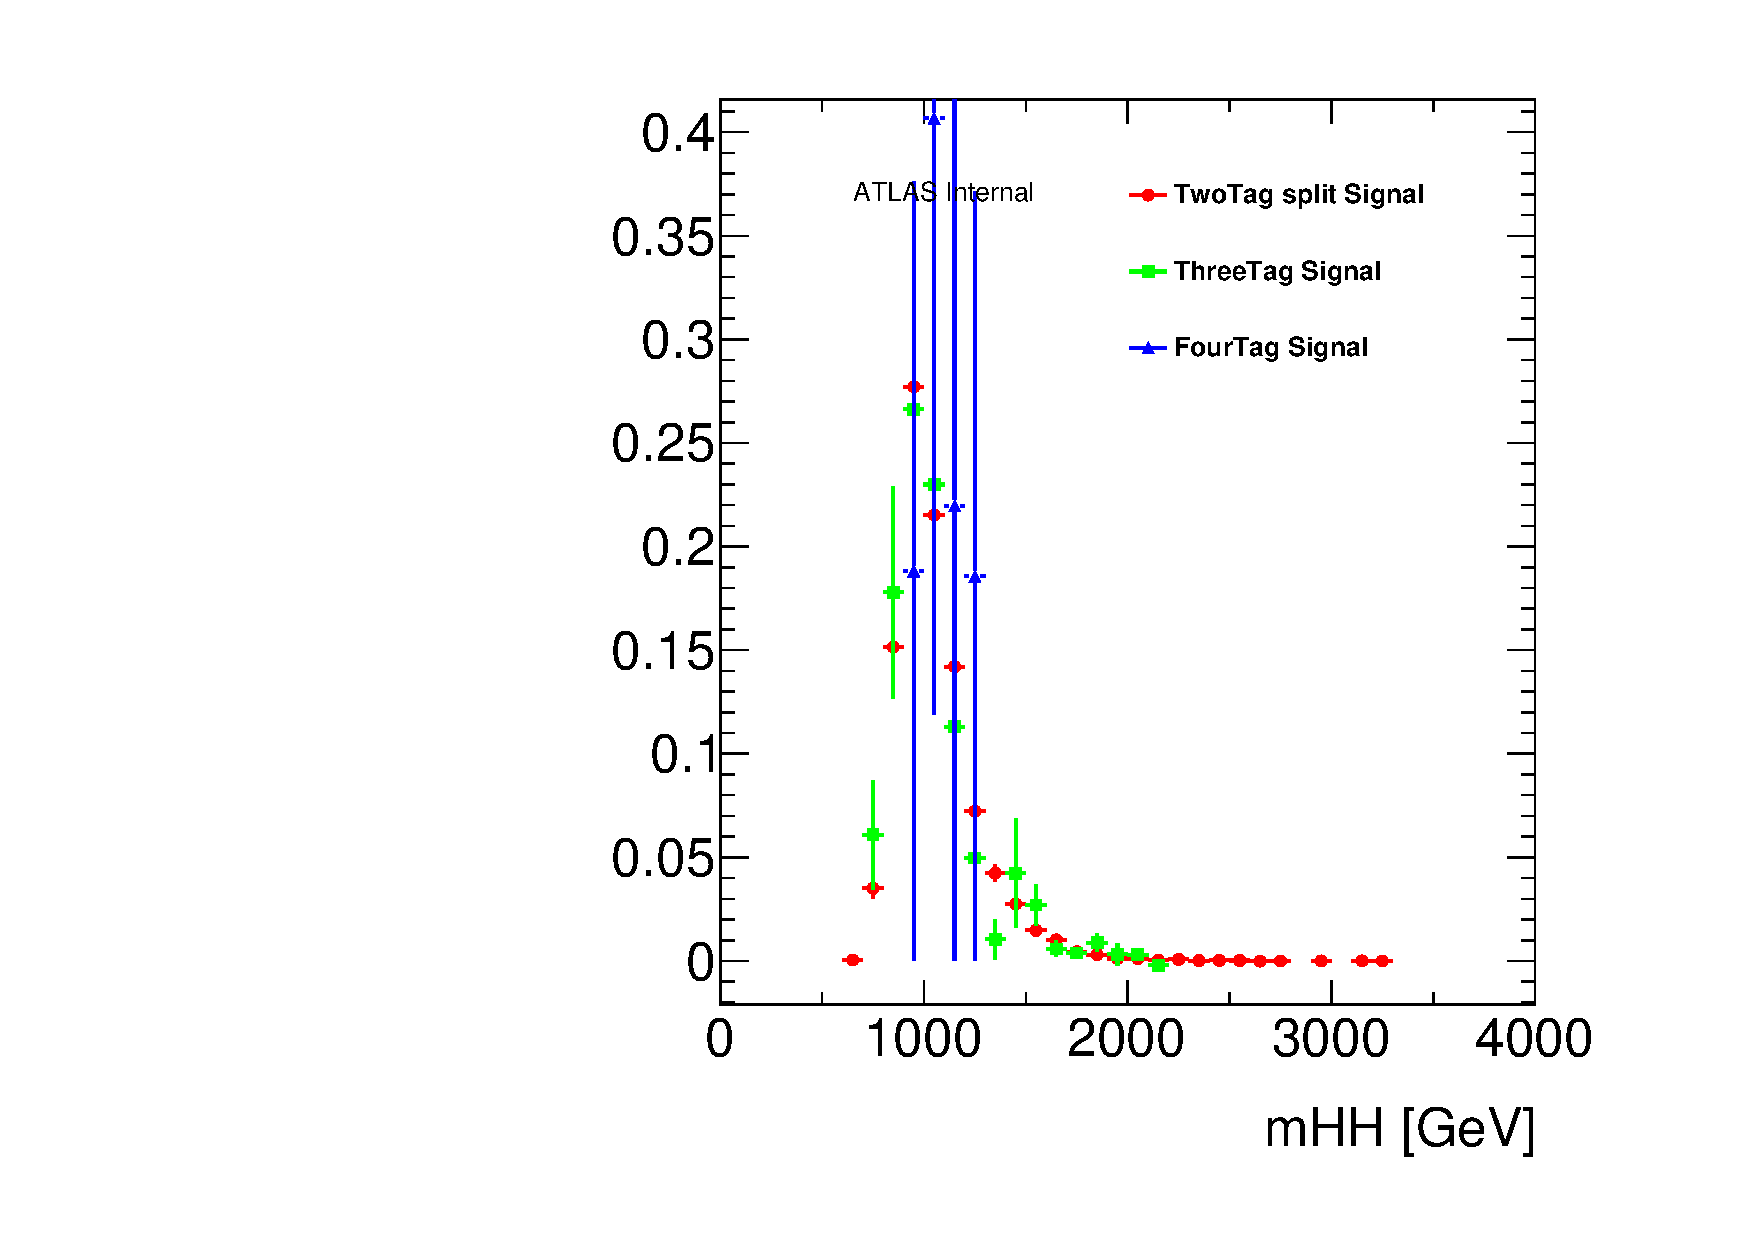
\includegraphics[angle=270, width=0.5\textwidth]{figures/boosted/Other/ttbar_compare_mHH_l.pdf}
\caption{comparison between the $2b$, $3b$, and $4b$ shapes for the di-large-$R$-jet mass distributions (the final discriminant) in the SR.}
\label{fig:ttshapeComp}
\end{center}
\end{figure}

%%%%%%%%%%%%%%%%%%%%%%%%%%%%%%%%%%%%%%%%%%%%%%%%%%%%%%%%%%%%%%%%%%%%%%%
%%%%%%%%%%%%%%%%%%%%%%%%%%%%%%%%%%%%%%%%%%%%%%%%%%%%%%%%%%%%%%%%%%%%%%%
%%%  Fitting
%%%%%%%%%%%%%%%%%%%%%%%%%%%%%%%%%%%%%%%%%%%%%%%%%%%%%%%%%%%%%%%%%%%%%%%
%%%%%%%%%%%%%%%%%%%%%%%%%%%%%%%%%%%%%%%%%%%%%%%%%%%%%%%%%%%%%%%%%%%%%%%

\pagebreak{}
\subsection{Fitting procedure for QCD and \ttbar\ normalization}
\label{sec:ttbarnorm}

\paragraph{}
The number of 4$b$/3$b$/2$b$s events in data observed in a given region (SB / CR / SR) can be described as:
\begin{eqnarray}\label{eq:fitparams}
N^{\nu_b}_{\text{data}} = \mu_{\text{qcd}}^{\nu_b} N^{xb}_{\text{qcd}} + \alpha_{t\bar{t}}^{\nu_b} N^{\nu_b}_{t\bar{t}} + N^{\nu_b}_{Z+jets}
\end{eqnarray}
where $\nu_b$ is the number of $b$-tagged track jets required, x is 1 for 2$b$s and 2 for 3$b$ and 4$b$. \muqcd\ is essentially an estimate of the ratio of the number of  QCD events with $\nu_b$ $b$-tagged track jets, to the number of $1b/2b$ QCD events, while the \ttbar\ normalization parameter $\alpha_{t\bar{t}}$\, applied after the \ttbar\ is scaled to the total integrated luminosity, is a correction to the MC prediction in this phase space. The same equation can be applied to the 4$b$/3$b$/2$b$s region (replacing $\nu_b$ by 4b/3b/2s $b$ in Equation~\ref{eq:fitparams}).   

\paragraph{}
In order to constrain the QCD and \ttbar\ background normalizations using data, a simultaneous fit is applied to extract both the \ttbar\ normalization with respect to the yields from simulation and the number of $1b/2b$ data events for the QCD background.  These scaling parameters are determined independently for the $4b/3b/2s$ signal regions. But as the procedure is the same for those three signal regions, we denote these scaling factors simply \muqcd and $\alpha_{t\bar{t}}$ in the following text.

\paragraph{}
A binned maximum likelihood fit is employed to find the values of \muqcd and $\alpha_{t\bar{t}}$, as well as the correlation between the two parameters. The fit is performed on the leading-\pt\ jet mass spectrum in the sideband region, as it has the best separation between QCD and \ttbar\ shapes. Due to the \pt$>450$ GeV cut imposed on the leading \largeR jet, the hadronic top quark is likely to be fully reconstructed inside of the \largeR jet and the leading jet mass in the \ttbar\ sample has a clean peak around $M=170$ GeV in the sideband region.

\paragraph{}
The values of \muqcd and $\alpha_{t\bar{t}}$ as estimated by the fits in the $4b/3b/2bs$ sideband regions can be found in Table~\ref{tab:bkgfit}, along with the correlation of the fitted parameters $\rho(\mu_{qcd},\alpha_{t\bar{t}}) = \frac{Cov(\mu_{qcd},\ \alpha_{t\bar{t}})}{\sigma_{\mu_{qcd}}\sigma_{\alpha_{t\bar{t}}} }$. \muqcd and $\alpha_{t\bar{t}}$ are approximately 70\% negatively correlated, which is not surprising as they are the only two components fit to the data distribution and their sum needs to predict the SB total event count.

\begin{table}[htbp!]
\begin{center}
\begin{footnotesize} 
\begin{tabular}{c|c|c|c} 
Sample & $\mu_{qcd}$ & $\alpha_{t\bar{t}}$ & $\rho(\mu_{qcd}, \alpha_{t\bar{t}})$ \\ 
\hline\hline 
FourTag & 0.033167 $\pm$ 0.0042799 & 0.89136 $\pm$ 0.59866 & -0.7846\\
ThreeTag & 0.16256 $\pm$ 0.0043405 & 0.79989 $\pm$ 0.073276 & -0.72029\\
TwoTag split & 0.062726 $\pm$ 0.00057307 & 0.98637 $\pm$ 0.018582 & -0.4698\\
\hline\hline 
\end{tabular} 
\end{footnotesize} 
\newline 

\caption{Background scaling parameters (\muqcd and $\alpha_{t\bar{t}}$) estimated from fits to the leading jet mass distributions in $4b/3b/2bs$ sideband regions. $\rho(\mu_{qcd},\alpha_{t\bar{t}}) = \frac{Cov(\mu_{qcd},\ \alpha_{t\bar{t}})}{\sigma_{\mu_{qcd}}\sigma_{\alpha_{t\bar{t}}} }$}
\label{tab:bkgfit}
\end{center}
\end{table}

\paragraph{}
Figure~\ref{fig:ttbar-fit} shows the post-fit spectrum of the leading \largeR calorimeter jet mass in the 4$b$/3$b$/2$b$s sideband regions. The normalization of \ttbar\ is 
constrained by the top quark mass peak around 170~GeV. The shapes of the data is also well modeled by the predicted background. The fitting errors on \muqcd and 
$\alpha_{t\bar{t}}$ are applied as systematic uncertainties taking into account their correlation. This will be explained in more detail in the systematics section.

\begin{figure}[htbp!]
\begin{center}
 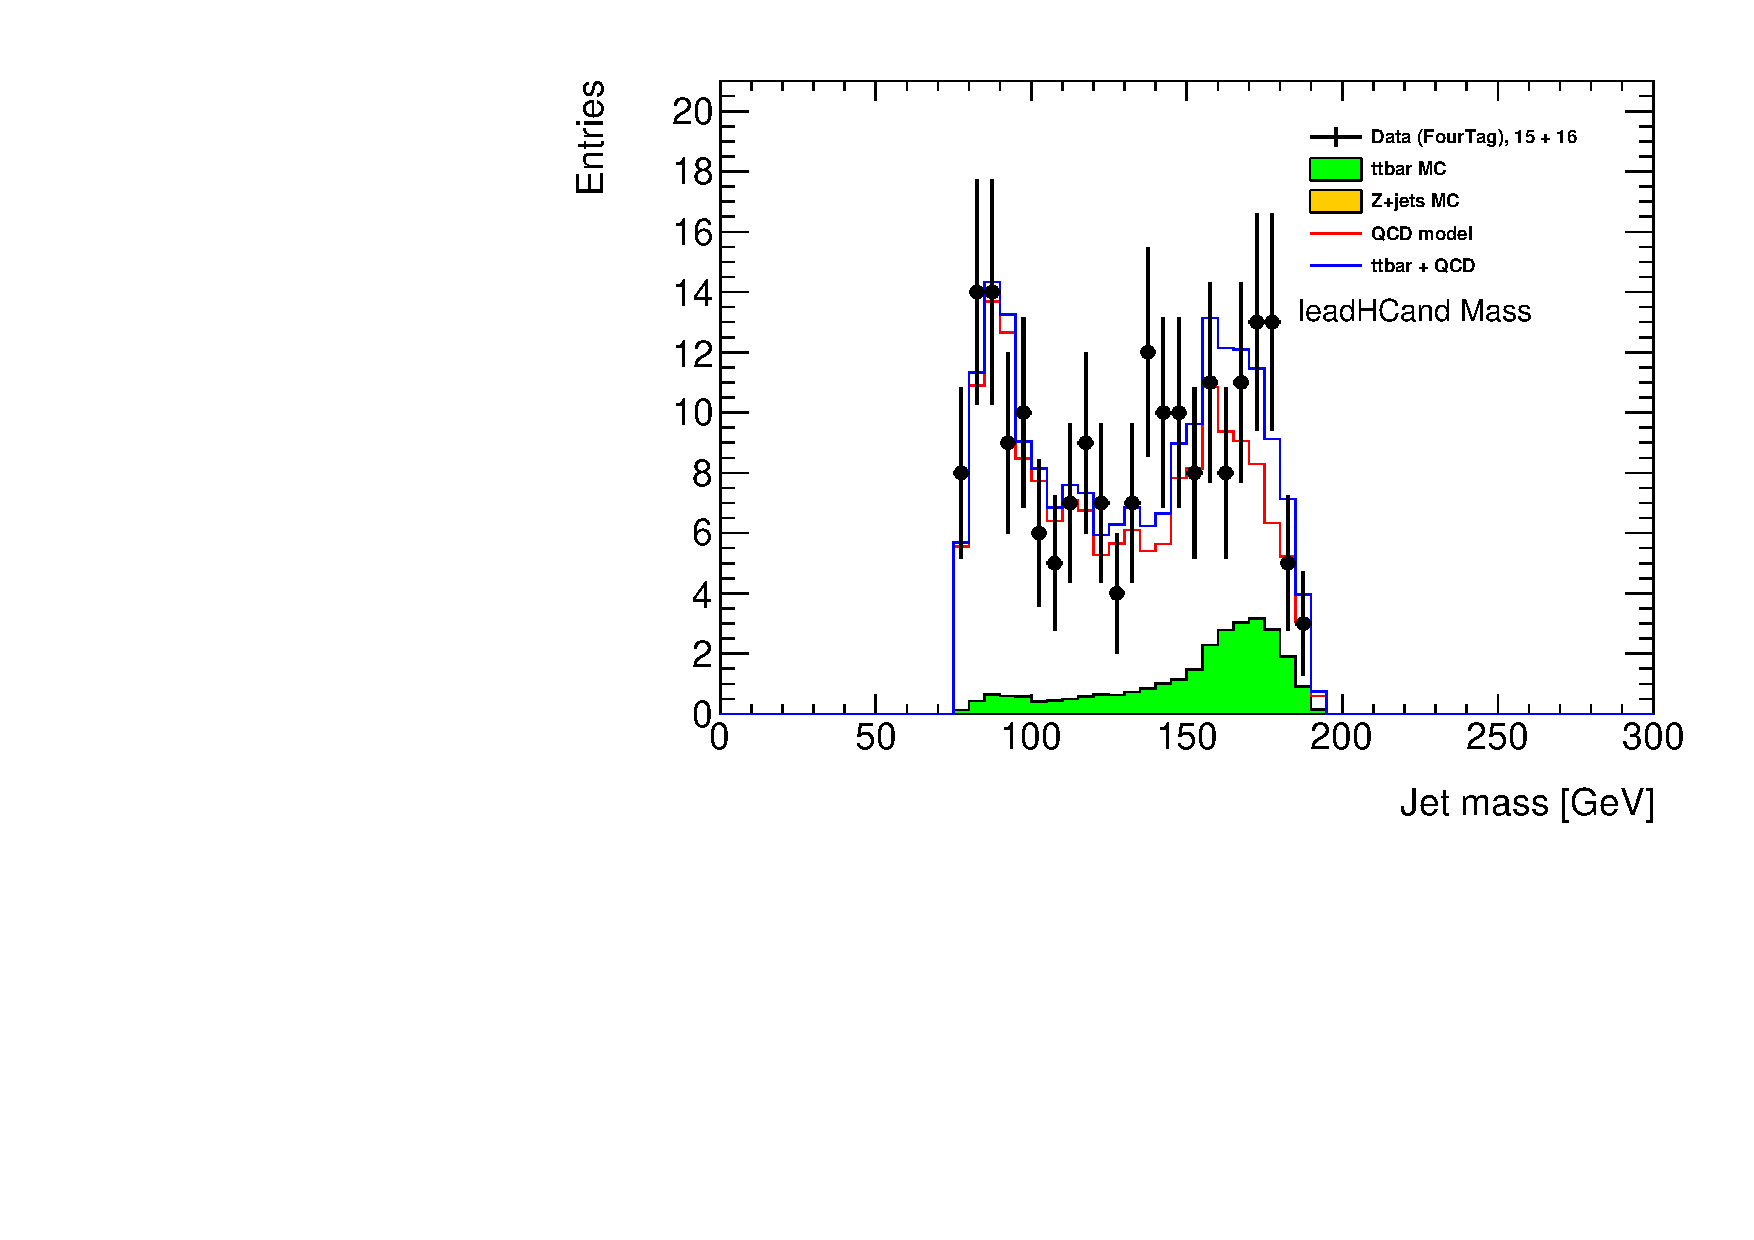
\includegraphics[angle=270, width=0.45\textwidth]{./figures/boosted/Fit/fitNorm_i4.pdf}\\
 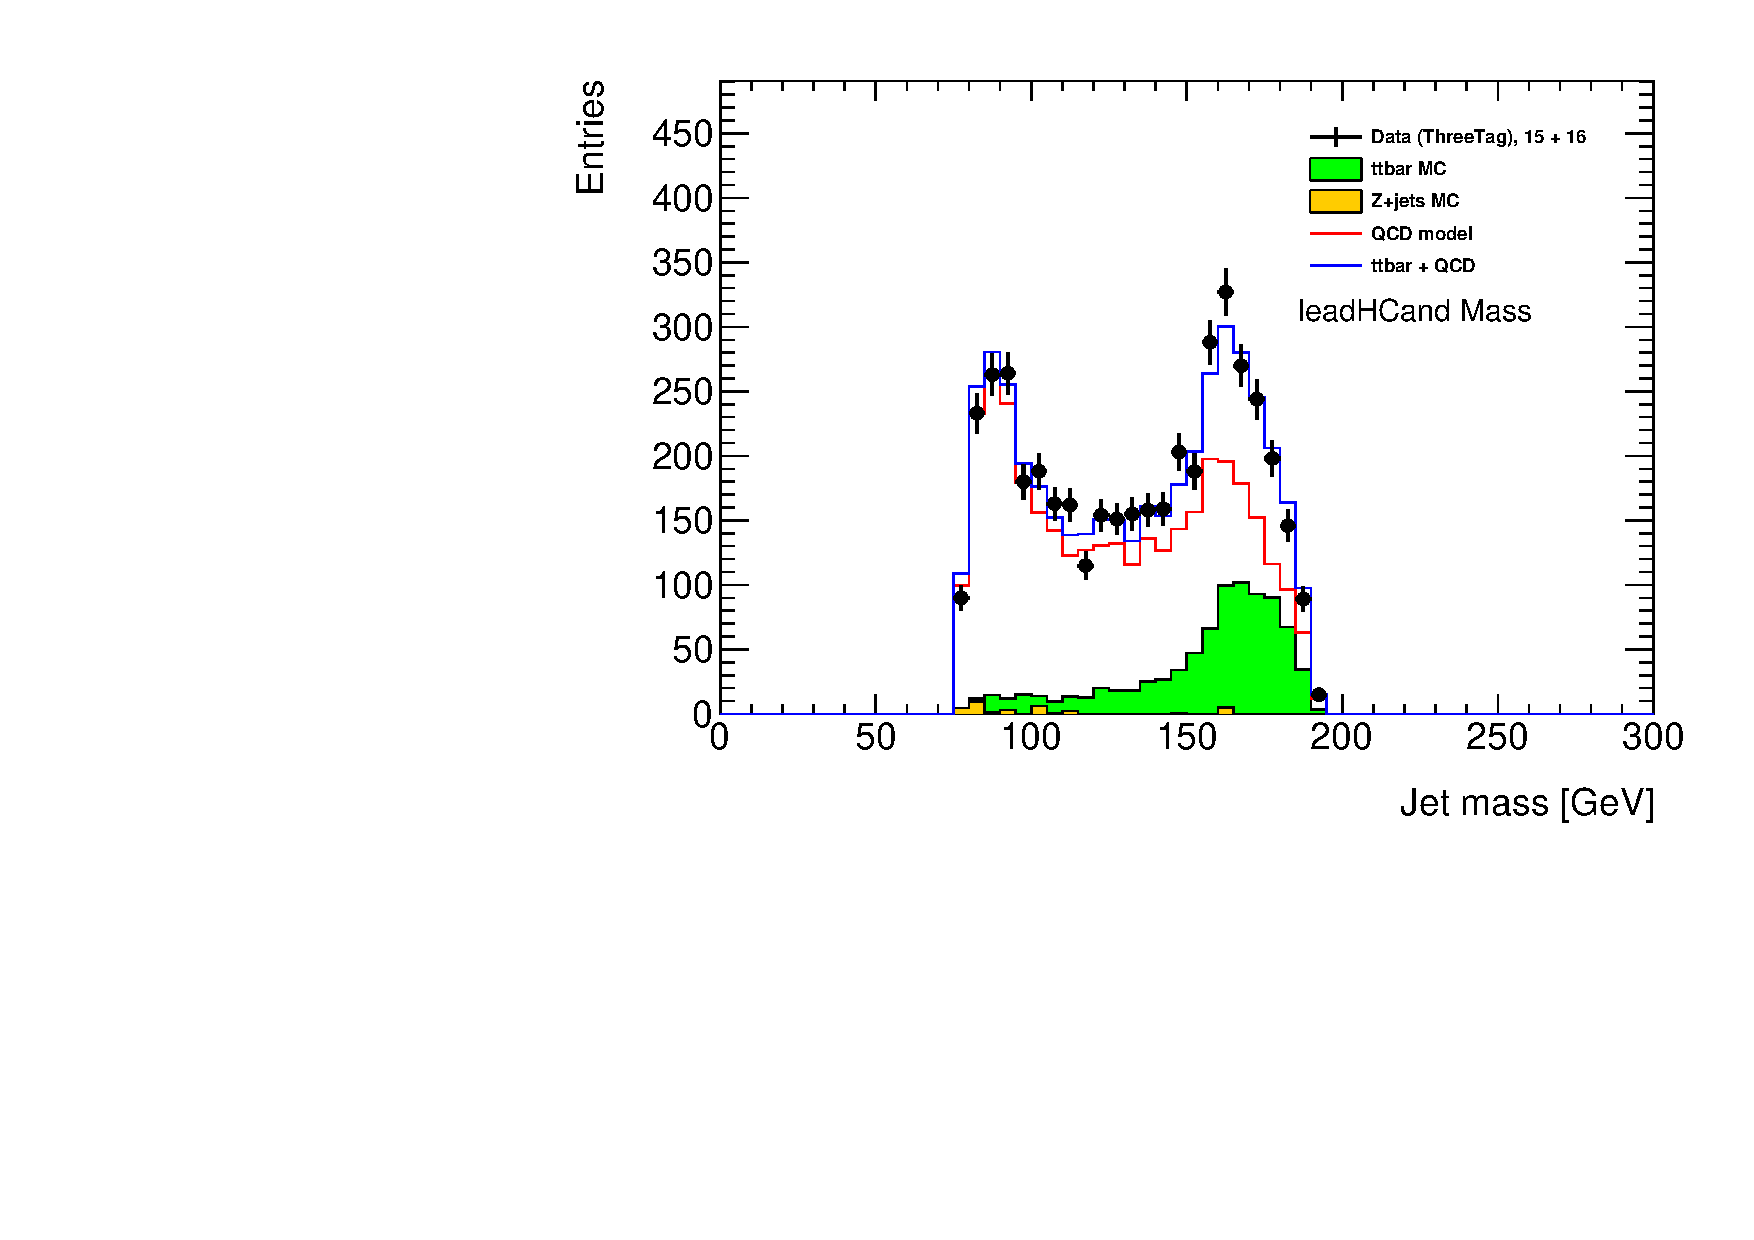
\includegraphics[angle=270, width=0.45\textwidth]{./figures/boosted/Fit/fitNorm_i3.pdf}\\
 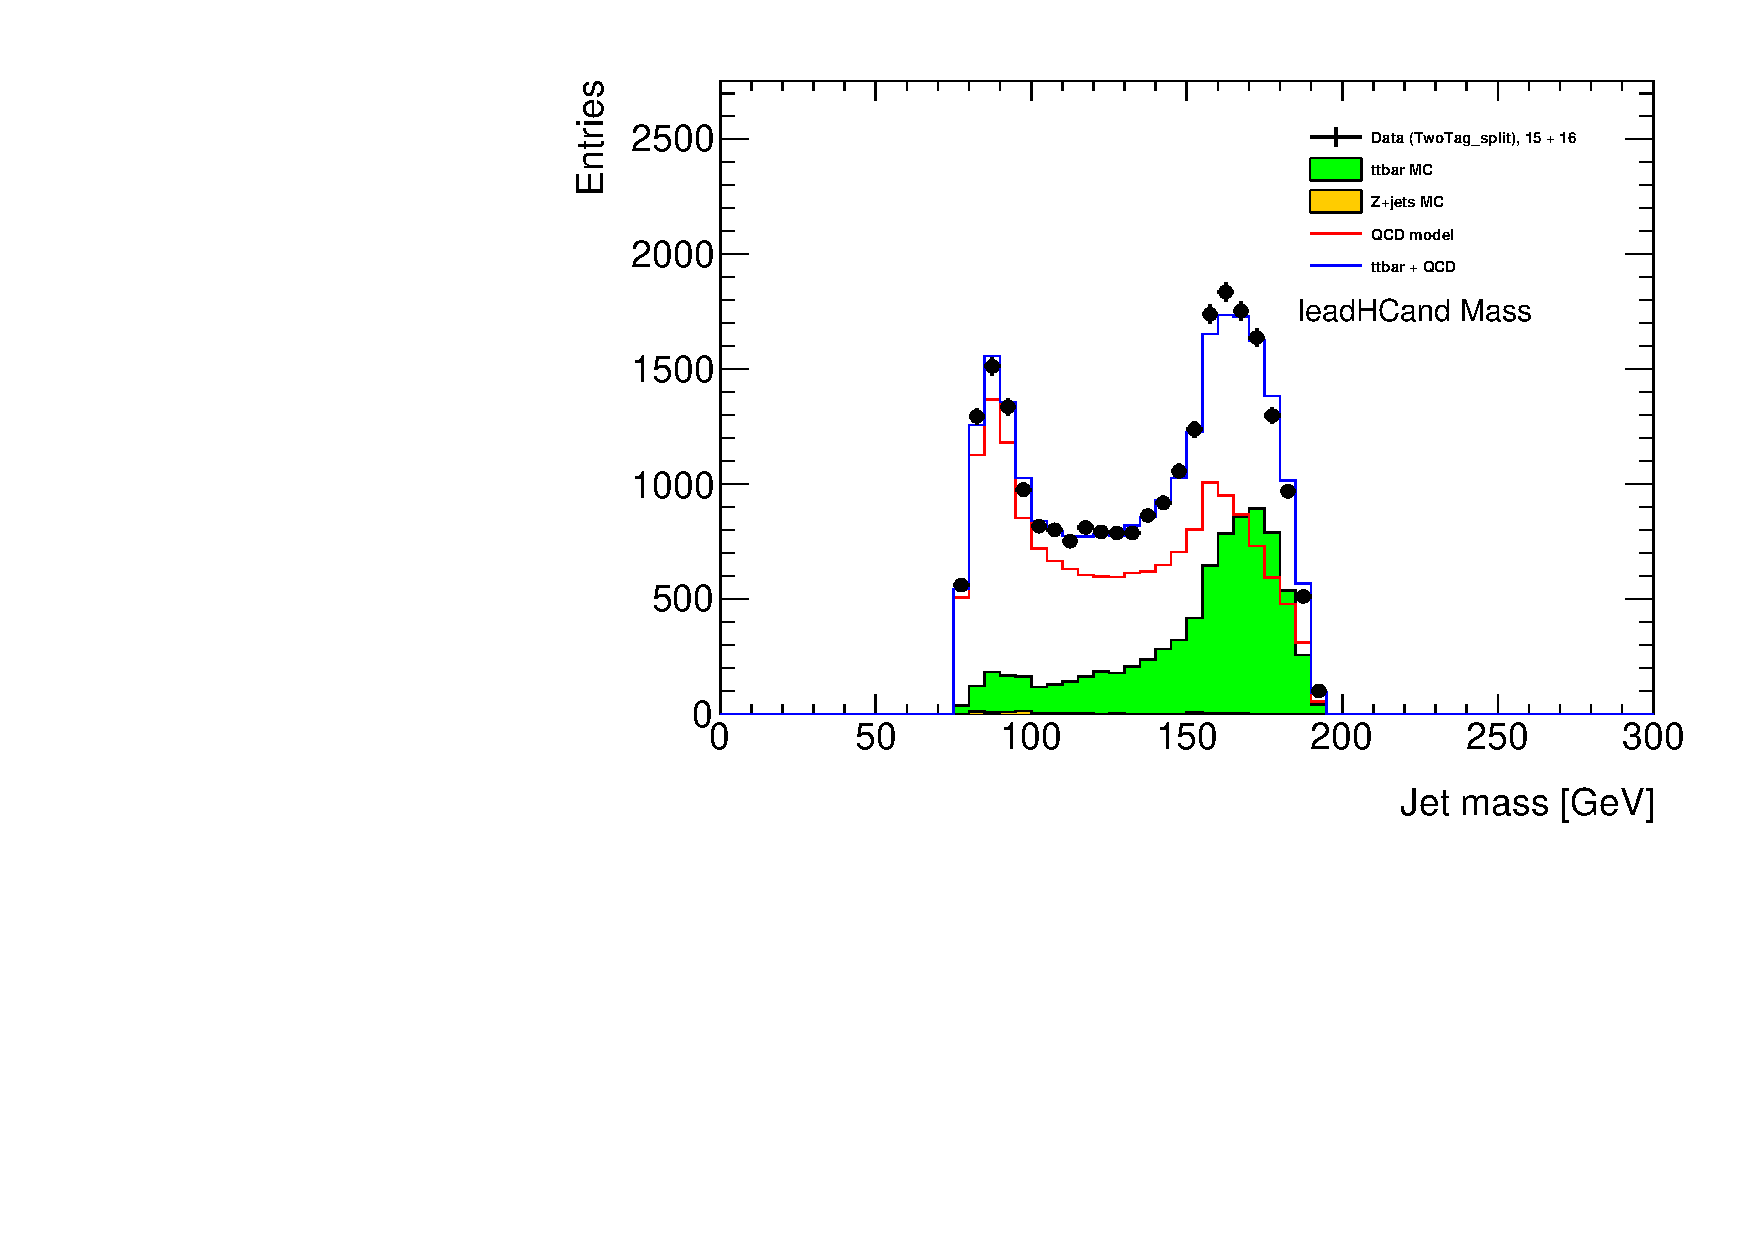
\includegraphics[angle=270, width=0.45\textwidth]{./figures/boosted/Fit/fitNorm_i2s.pdf}\\
\caption{Simultaneous fit of \muqcd and \alphatt in 4$b$ (top) and 3$b$ (middle) and $2b$ (bottom) sideband region using leading \largeR calorimeter jet mass spectrum.}
\label{fig:ttbar-fit}
\end{center}
\end{figure}

\clearpage

%%%%%%%%%%%%%%%%%%%%%%%%%%%%%%%%%%%%%%%%%%%%%%%%%%%%%%%%%%%%%%%%%%%%%%%
%%%%%%%%%%%%%%%%%%%%%%%%%%%%%%%%%%%%%%%%%%%%%%%%%%%%%%%%%%%%%%%%%%%%%%%
%%%  Reweighting
%%%%%%%%%%%%%%%%%%%%%%%%%%%%%%%%%%%%%%%%%%%%%%%%%%%%%%%%%%%%%%%%%%%%%%%
%%%%%%%%%%%%%%%%%%%%%%%%%%%%%%%%%%%%%%%%%%%%%%%%%%%%%%%%%%%%%%%%%%%%%%%

\subsection{Kinematic reweighting}
\label{sec:boosted-reweight}
%%\paragraph{}
Due to the large contribution from the completely data-driven QCD background, it is important to model this background as good as possible in all regions of the analysis. Using the $1/2b$ region to model the 2$b$s, 3$b$, and 4$b$ regions can introduce discrepancies in the modeling of the estimated QCD background versus the real n$b$ data. These discrepancies arise possibly from the non-trivial effect that $b$-tagging has on jet kinematics. The natural choice of reweighting variable is the $p_{T}$ of the track jets in the event, since these are the objects that we apply the $b$-tagging to. Also, large-$R$ jet $p_{T}$ is also reweighted to account for the effect from light and charm quark composition difference at different energy scales. The three chosen variables are the leading large-$R$ jet $p_{T}$, leading large-$R$ jet leading trackjet $p_{T}$ and subleading large-$R$ jet leading trackjet $p_{T}$.

%%\paragraph{}
In order to account for the $b$-tagging effect, a reweighting on the $1/2b$ data is adopted. The basic idea is to reweight the non $b$-tagged Higgs candidate to have kinematic distributions just like a $b$-tagged Higgs candidate. The idea is demonstrated in Figure~\ref{fig:rw-2bs-comp}. It shows that 2$b$s has very similar kinematic distributions on the trackjet \pt as the 1$b$ sample, when the variable is the $b$ tagged trackjet. 

%%\paragraph{}
For 2$b$s, the 1$b$ non-tagged Higgs candidate is reweighted to be like a 1$b$ tagged Higgs candiate; for 3$b$, the 2$b$ non-tagged Higgs candidate is reweighted to be like a 1$b$ tagged Higgs candidate; for 4$b$, the 2$b$ non-tagged Higgs candidate is reweighted to be like a 2$b$ tagged Higgs candidate. For each category, the events are split into two orthogonal subgroups, depending on whether leading/subleading Higgs candidate is $b$-tagged, the event is then reweighted such that the untagged Higgs candidate's distribution behaves like the corresponding $b$-tagged Higgs candidate's.

%%%%%%%%%%%%%%%%%%%%%%%%%%%
\begin{figure*}[htbp!]
\begin{center}
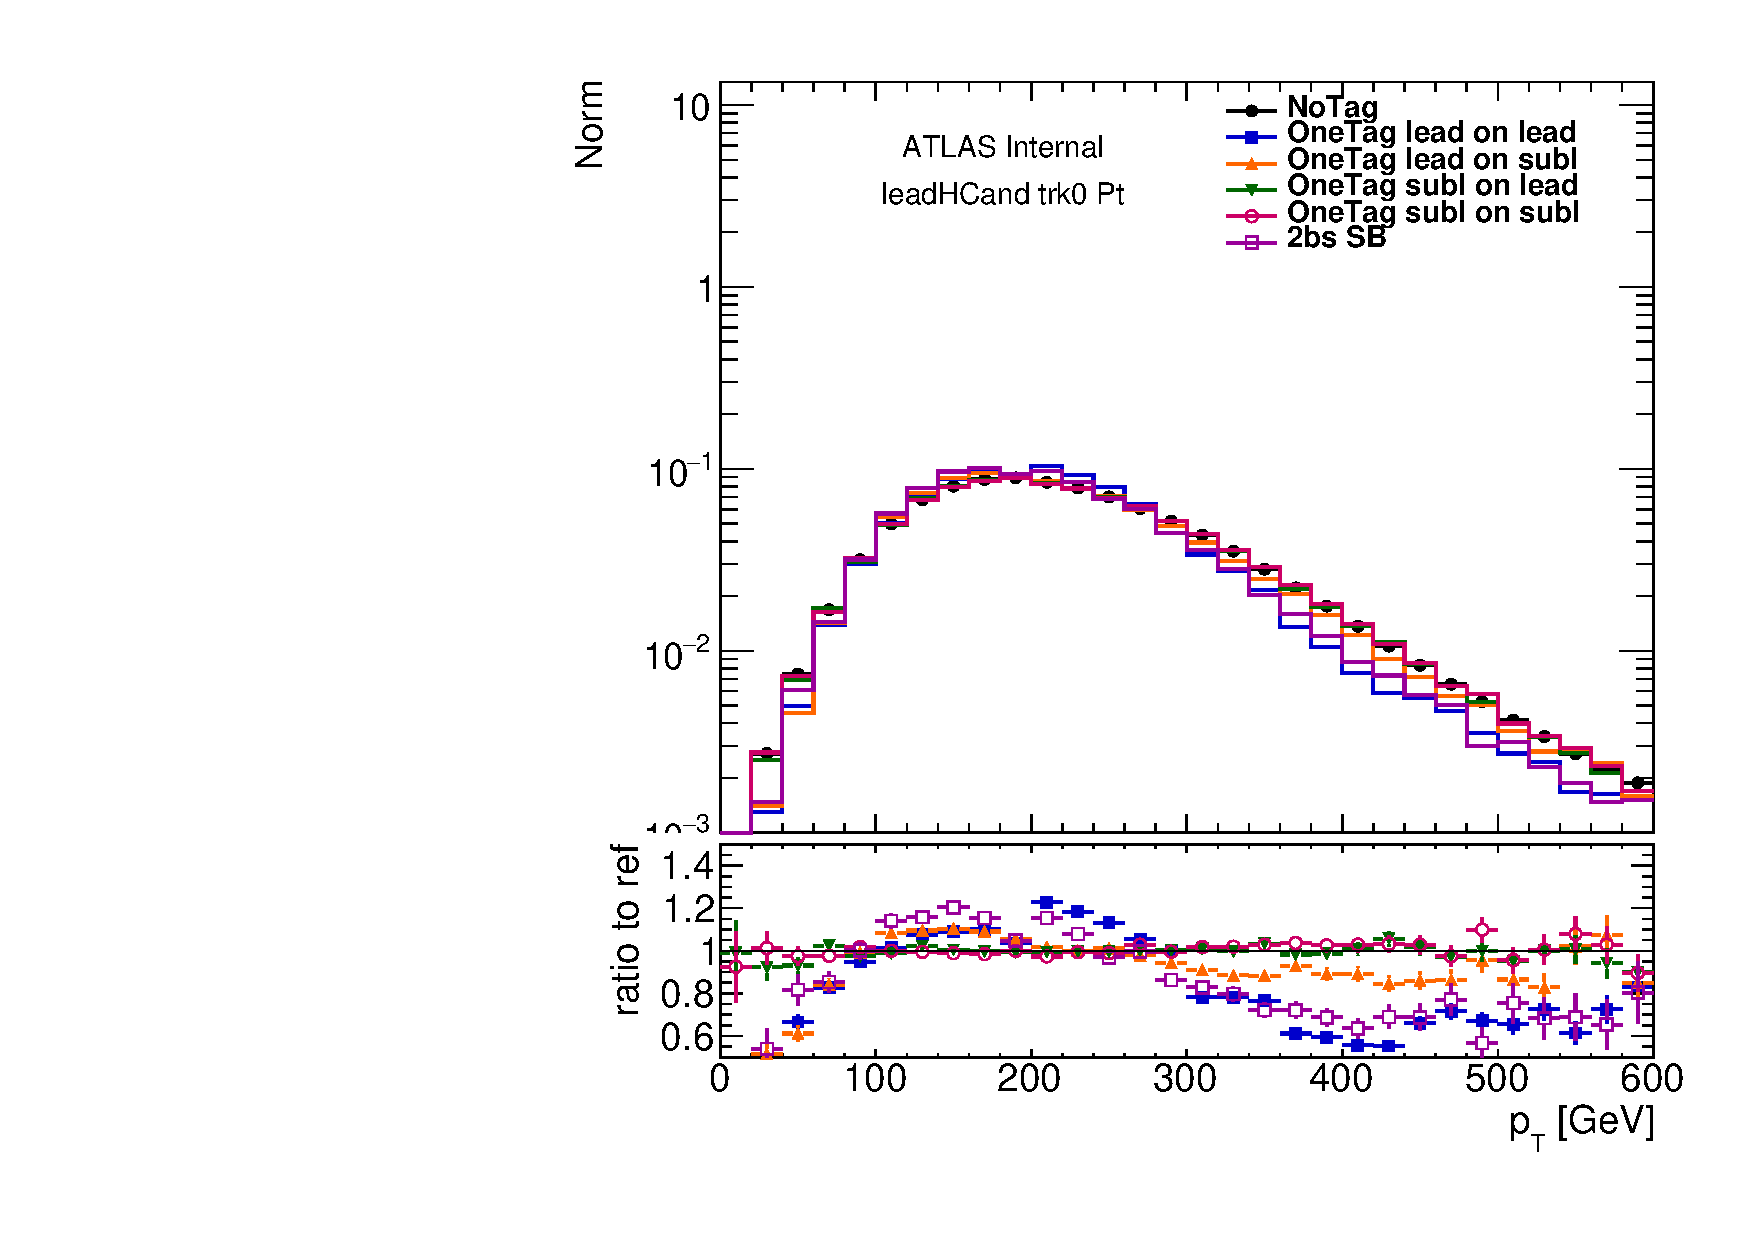
\includegraphics[width=0.4\textwidth,angle=-90]{figures/boosted/Prereweight/2bs_directcompare_leadHCand_trk0_Pt_1.pdf}
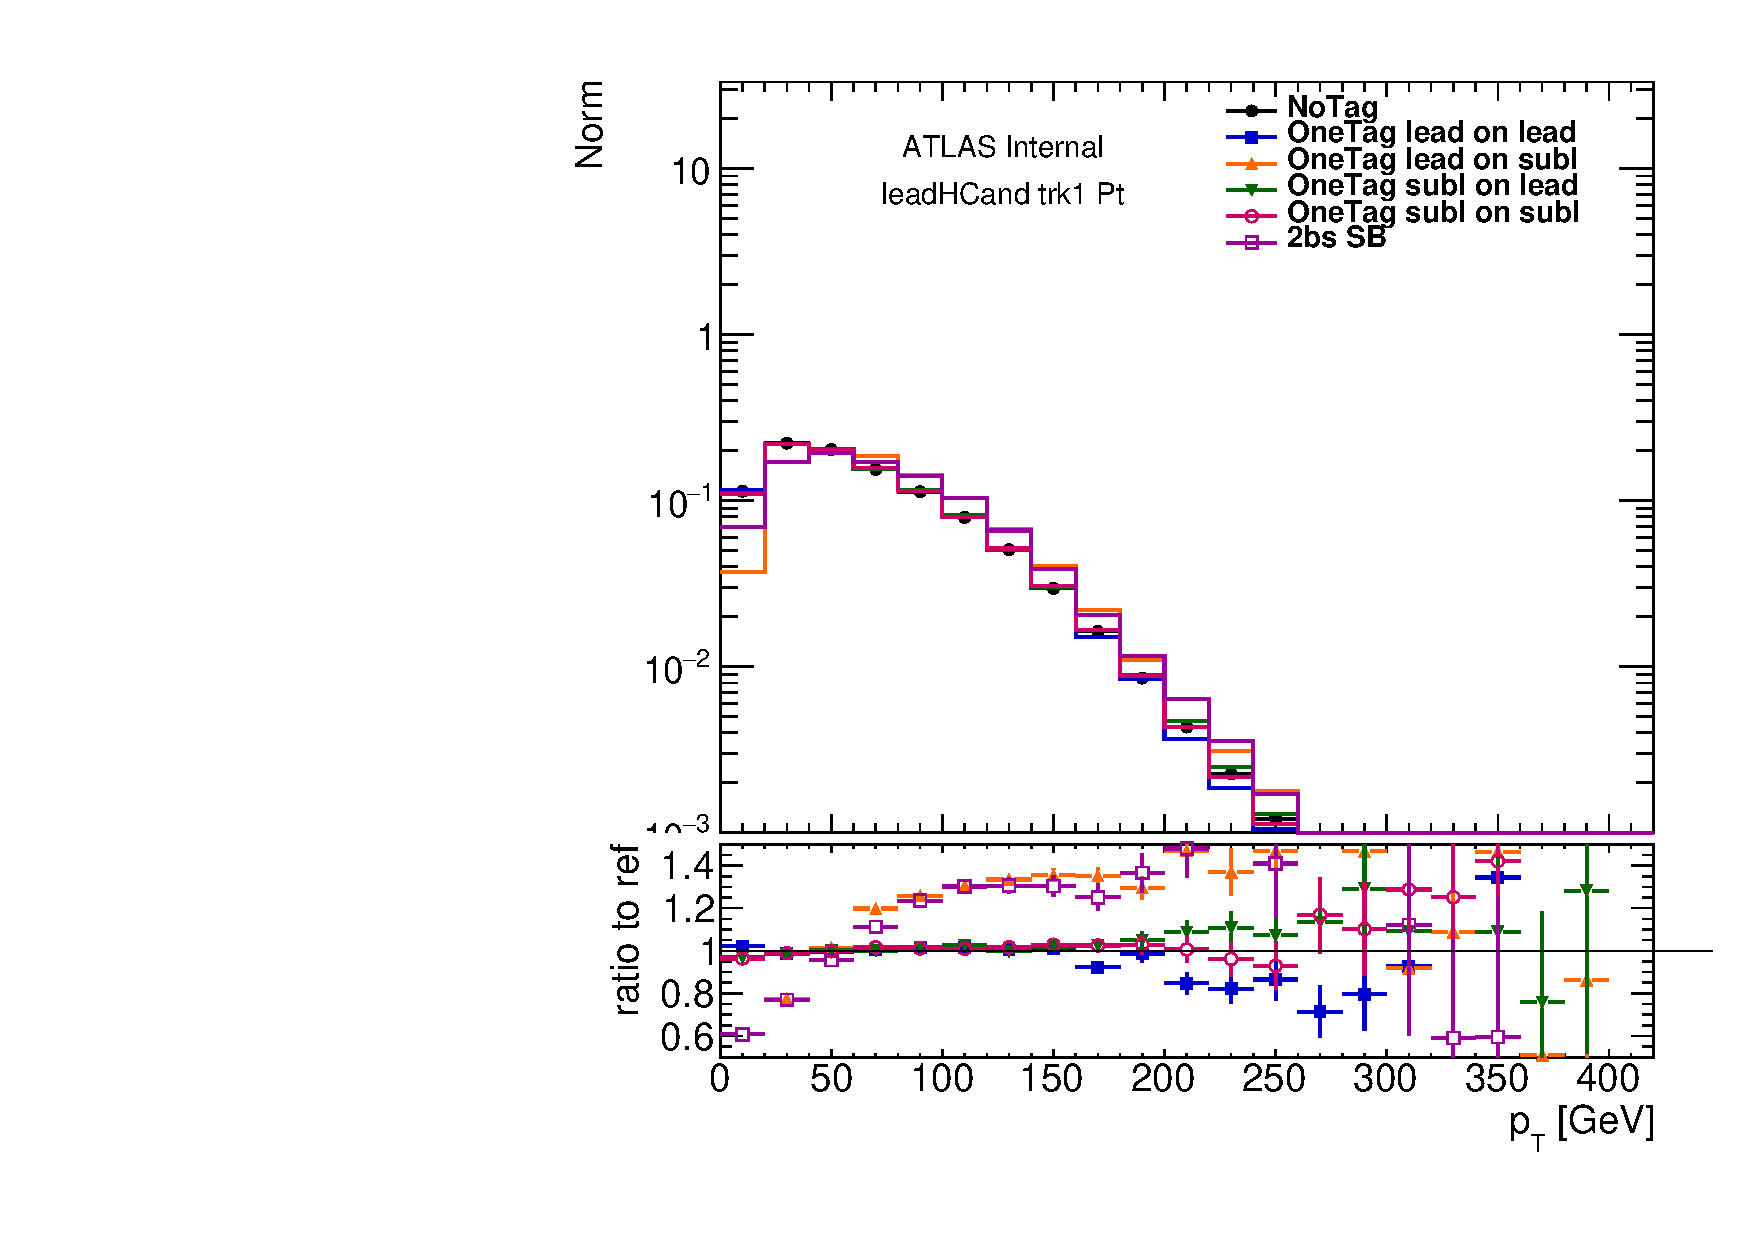
\includegraphics[width=0.4\textwidth,angle=-90]{figures/boosted/Prereweight/2bs_directcompare_leadHCand_trk1_Pt_1.pdf}\\
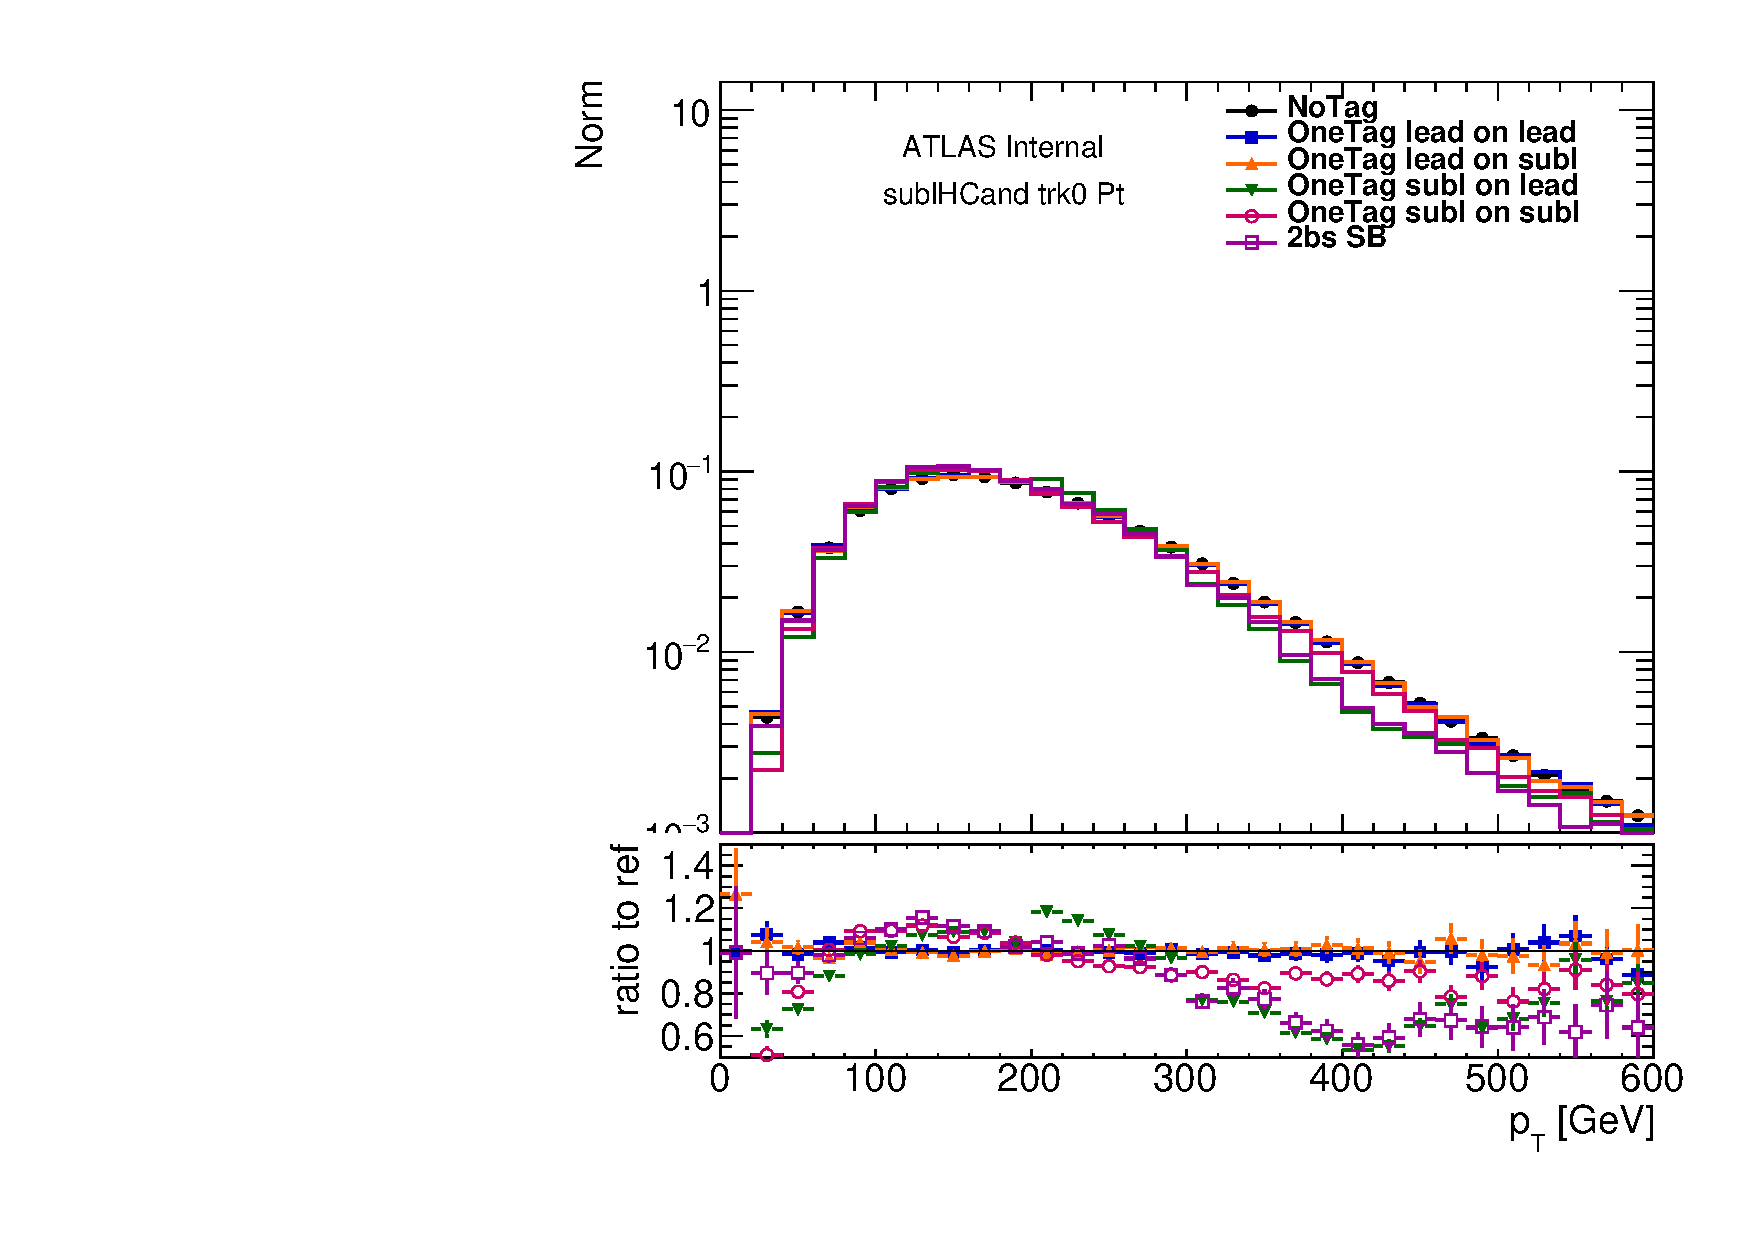
\includegraphics[width=0.4\textwidth,angle=-90]{figures/boosted/Prereweight/2bs_directcompare_sublHCand_trk0_Pt_1.pdf}
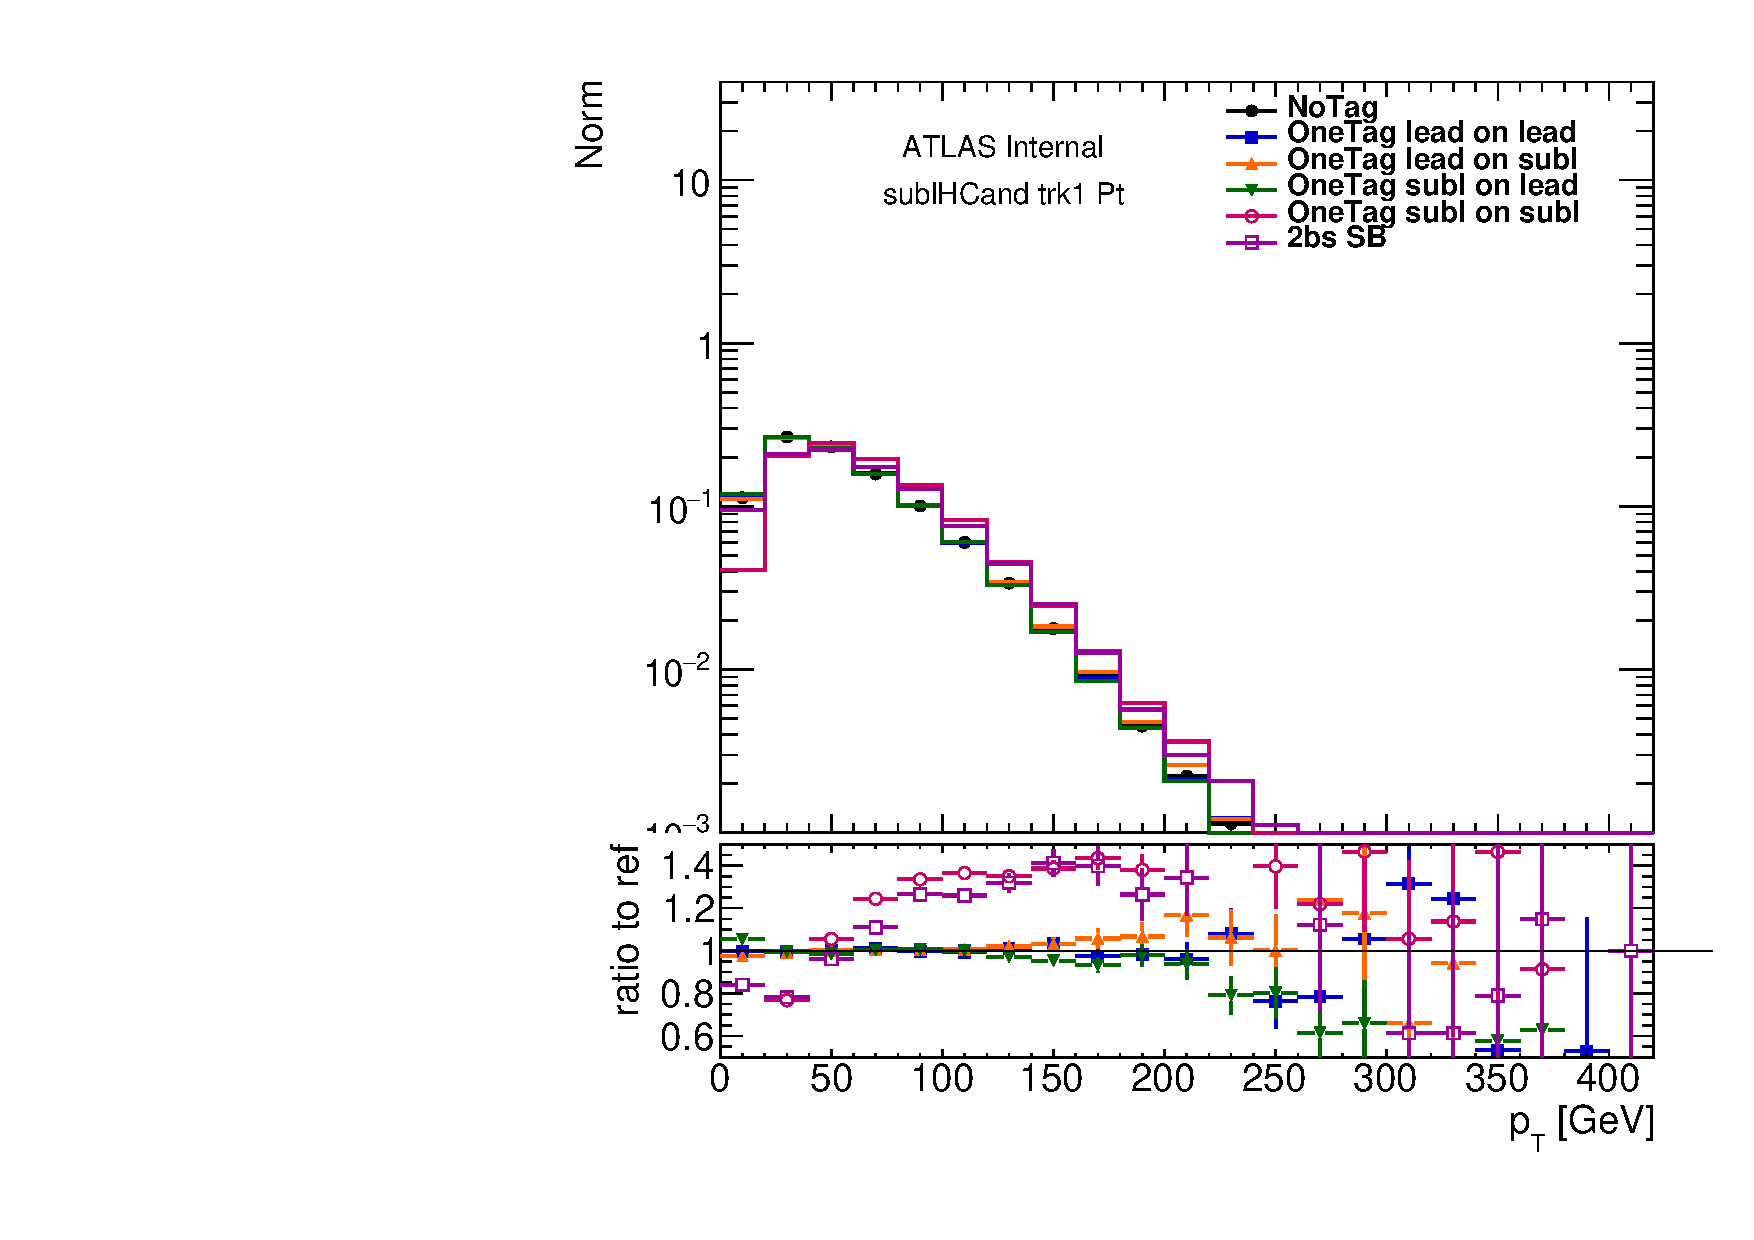
\includegraphics[width=0.4\textwidth,angle=-90]{figures/boosted/Prereweight/2bs_directcompare_sublHCand_trk1_Pt_1.pdf}\\
\caption{Comparison of different trackjet \pt distributions. Top row is for leading \pt Higgs candidate, and bottom row is for subleading \pt Higgs candidate. Left column is for the leading \pt trackjet of the Higgs candidate, and right column is for the subleading \pt trackjet of the Higgs candidate. Shown in the plot are just data distributions, inclusive of SB, CR, and SR regions for 0$b$ and 1$b$, while for 2$b$s only the SB region is shown. 1$b$ sample is further split into four subcategories, depending on which trackjet gets $b$ tagged. OneTag lead on lead means the $b$ tagged trackjet is the leading trackjet of the leading Higgs candidate, OneTag lead on subl means the $b$ tagged trackjet is the subleading trackjet of the leading Higgs candidate, OneTag subl on lead means the $b$ tagged trackjet is the leading trackjet of the subleading Higgs candidate, and OneTag subl on subl means the $b$ tagged trackjet is the subleading trackjet of the subleading Higgs candidate. At the bottom ratio plot, all the ratio are taken with respect to the 0$b$ tagged distribution.}
\label{fig:rw-2bs-comp}
\end{center}
\end{figure*}

%%\paragraph{}
To avoid potential biases in the final distributions used for the analysis, a reweighting technique is applied to the $1/2b$ data only. Since each signal region is modeled by a different $1/2b$ tag category: 2$b$s by 1$b$ tag events with at least 1 track jets on both large-$R$ jets, 3$b$ by 2$b$ tag events with at least one track jets on one large-$R$ jet and at least two track jets on the other large-$R$ jet, and 4$b$ by 2$b$ tag events with at least two track jets on both large-$R$ jets, the reweighting procedure is the same but orthogonal for the three different channels. Note the 2$b$ sample is already split into seperate parts, as described in paragraph \ref{par:boosted-qcd-2bseperate}.

\clearpage{}
%%\paragraph{}
The detailed procedure is listed as follows:
\begin{itemize}
\item Substracting $1/2b$ tag $t\bar{t}$ and $Z+$jets samples in the sideband from the $1/2b$ tag data in the Sideband + Control + Signal regions to get the $1/2b$ QCD inclusive estimate.
\item Seperate the $1/2b$ tag sample further to sample: A. that has the $b$-tagged Higgs is the leading \pt Higgs candidate, and B. that the $b$-tagged Higgs is the subleading \pt Higgs candidate.
\item For each variable, i.e. the large-$R$ jet $p_{T}$, normalize sample A to sample B total number of events, take the ratio of sample A distribution over sample B distribution, and fit the ratio with a spline function. (TSpline3)
\item Use this functional form to extract reweighting values for each variable that is considered. The reweighting value for each variable is also constrained to be within a $-30\%$ to $+40\%$ range compared to one, to avoid over corrections and failed fit situations. 
%Then, the difference from one is scaled by $0.618$ (the golden ratio) to get a new weight, which is applied later. This accounts for over correlation by the spline and accerlerates convergence.
\item For each event, all the weights are multiplied together to change the $1/2b$ tag data event weight. Another constraint is applied, such that each total reweighting value is constrained to be within a $10\%$ to $+1000\%$ range compared to one, again to avoid over corrections.
\item The reweighting is done on the three variables: large-$R$ jet $p_{T}$ and the two track jet $p_{T}$s, which is counted as one iteration of reweighting.
\item A total of ten iterations are used to stabalize the reweighting. The reweighting is roughly converging after three iterations.
\end{itemize}

%%\paragraph{}
For reweighting method comparisons and validations in data and Dijet MC, see Appendix~\ref{app:reweightstudy}.

\subsubsection{Reweighting Fits}
\label{sec:boosted-Reweight-Fit}
%%\paragraph{}
The first iteration, second iteration, and last iteration of fits for 2$b$s, where in 1$b$ data, the non-tagged Higgs candidate are reweighted to be like a 1$b$ tagged Higgs candidate, can be seen in Figure~\ref{fig:rw-2bs-lead} and ~\ref{fig:rw-2bs-subl}. Similar distributions for 3$b$, where in 2$b$ data, the non-tagged Higgs candidate are reweighted to be like a 1$b$ tagged Higgs candidate, are shown in Figure~\ref{fig:rw-3b-lead} and ~\ref{fig:rw-3b-subl}. Similar distributions for 4$b$, where in 2$b$ data, the non-tagged Higgs candidate are reweighted to be like a 2$b$ tagged Higgs candidate, are shown in Figure~\ref{fig:rw-4b-lead} and ~\ref{fig:rw-4b-subl}. The before reweighting distribution (first row), the reweighting result after the first interation (second row), and the final distribution after reweighting (last row) are presented.

%%\paragraph{}
It should be noted that in the some plots, like Figure~\ref{fig:rw-4b-lead} and ~\ref{fig:rw-4b-subl}, the last ratio bin sometimes still doesn't converge to unity. This is a feature from the limited statistics from the last bin, especially in the 4$b$ case, where only $20\%$ number of events in 2$b$ is used for background prediction and therefore reweighted. One could choose a different binning and use more iterations to help this converge to one, yet the last bin's few event will also likely to end up with a large unphysical weight and therefore harm the background prediction later.

%%\paragraph{}
For the distribution of weights and the weight as a function of different kinematic ranges, see Appendix~\ref{app:reweight-dist}.
%%%%%%%%%%%%%%%%%%%%%%%%%%% original distributions
\begin{figure*}[htbp!]
\begin{center}
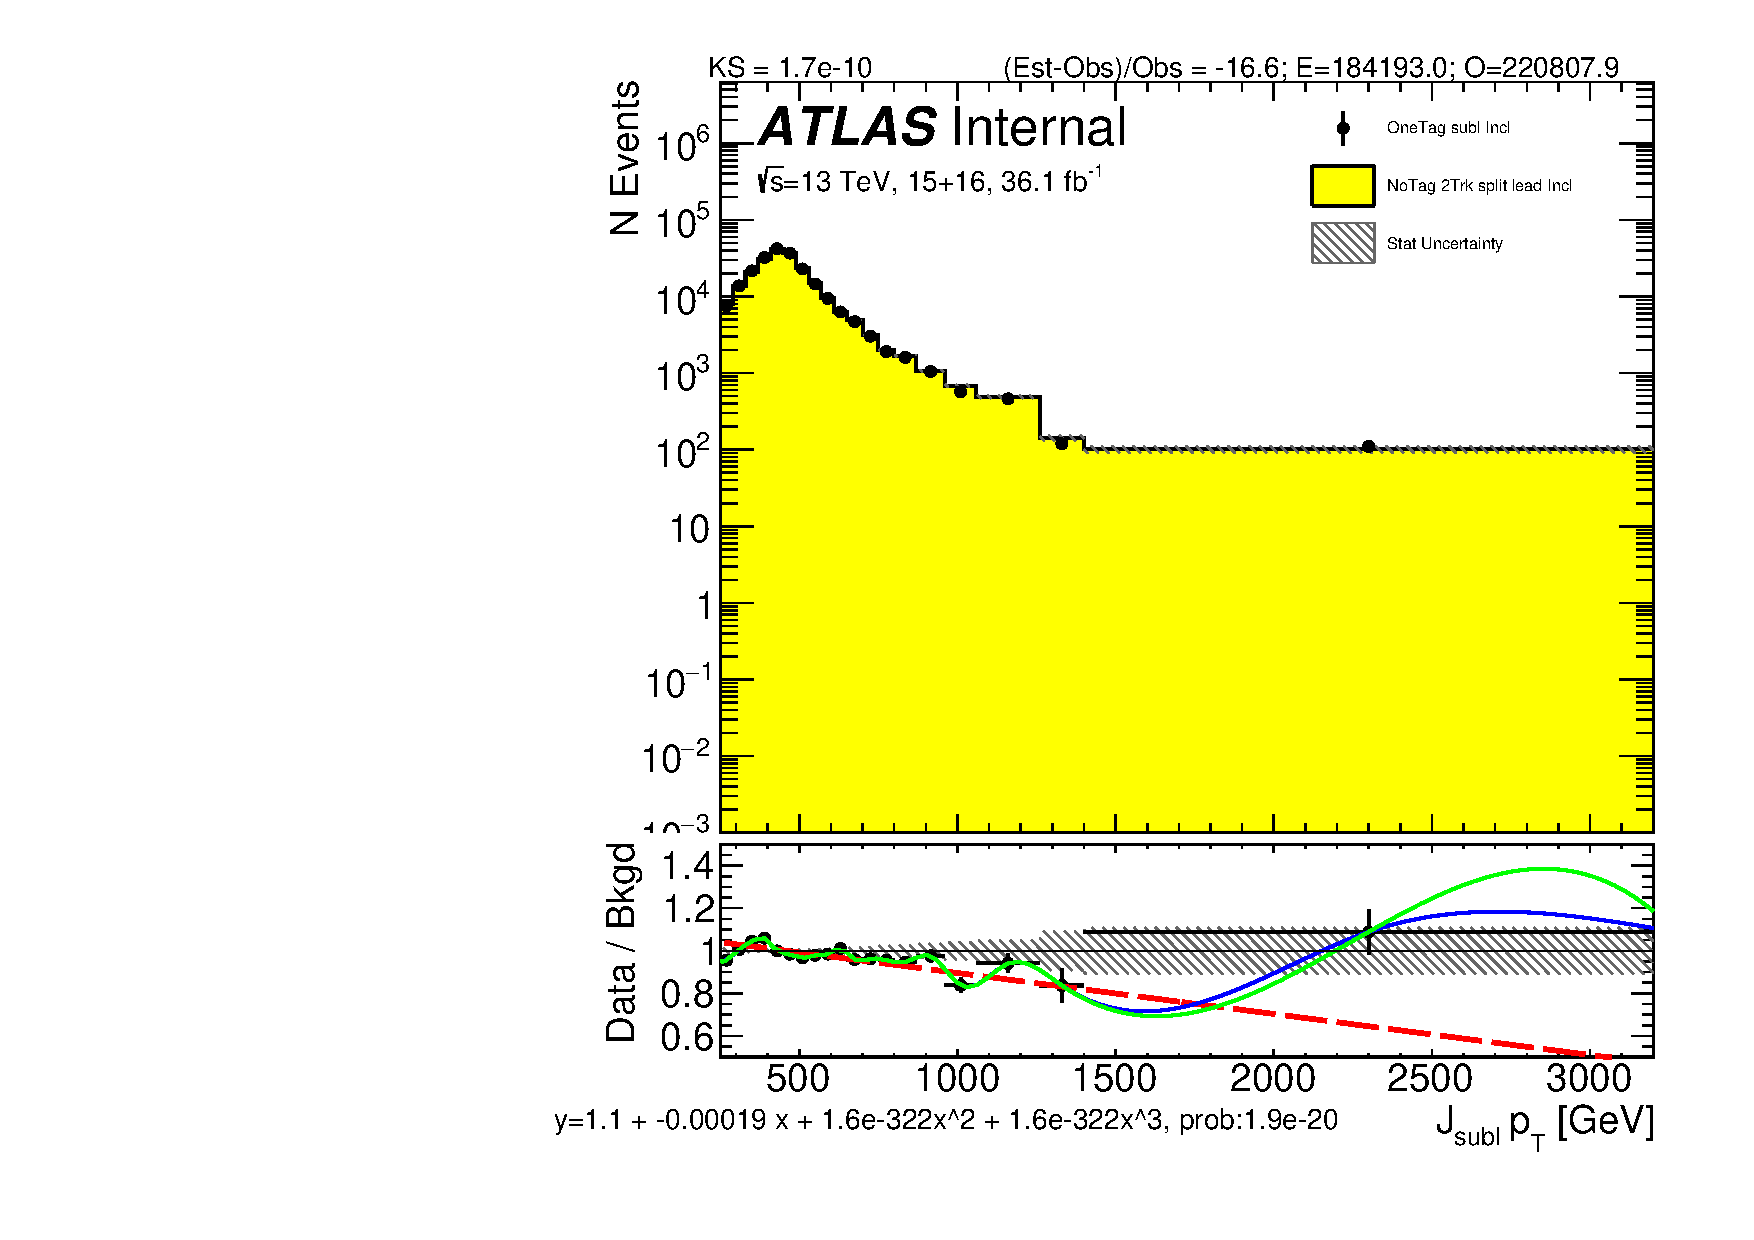
\includegraphics[width=0.32\textwidth,angle=-90]{figures/boosted/Reweight/Fits/Moriond_NoTag_2Trk_split_lead_Incl_sublHCand_Pt_m_1.pdf}
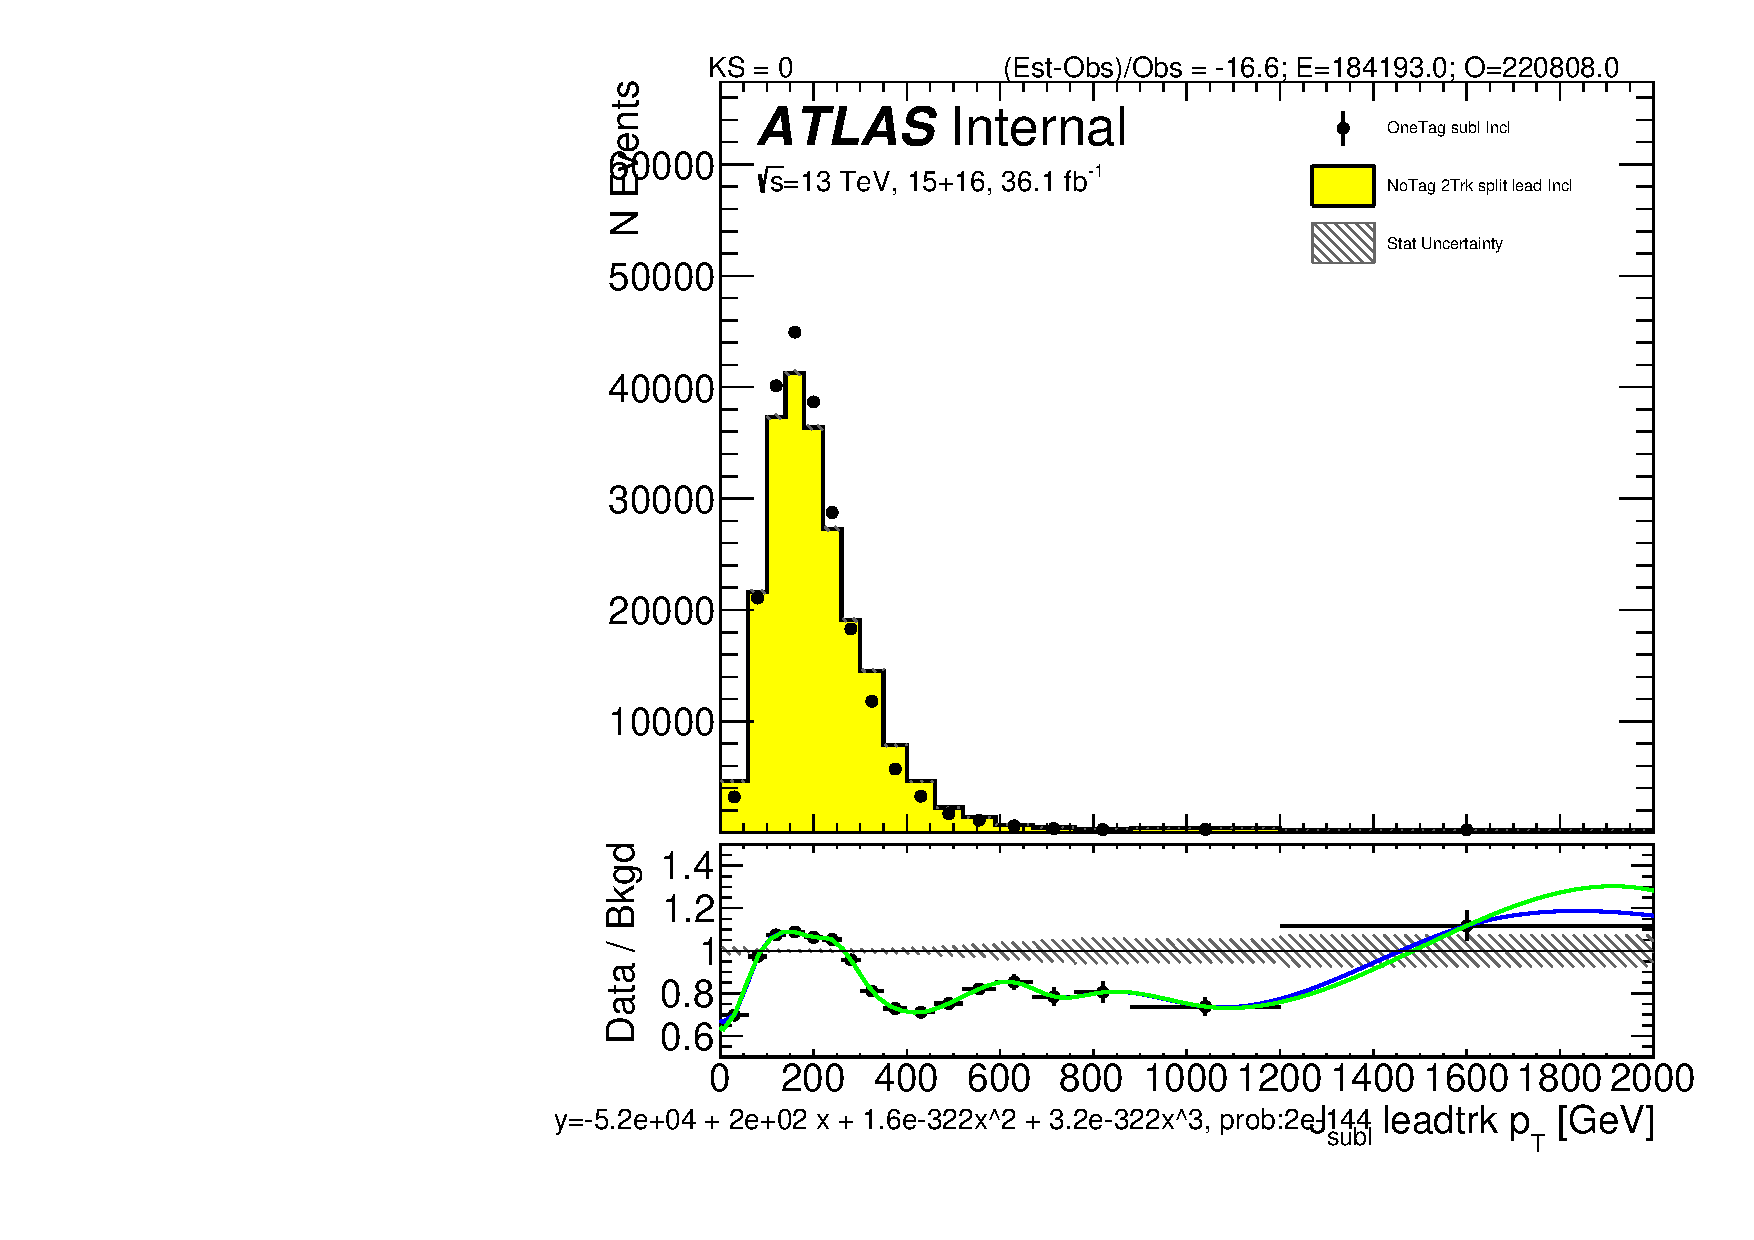
\includegraphics[width=0.32\textwidth,angle=-90]{figures/boosted/Reweight/Fits/Moriond_NoTag_2Trk_split_lead_Incl_sublHCand_trk0_Pt.pdf}
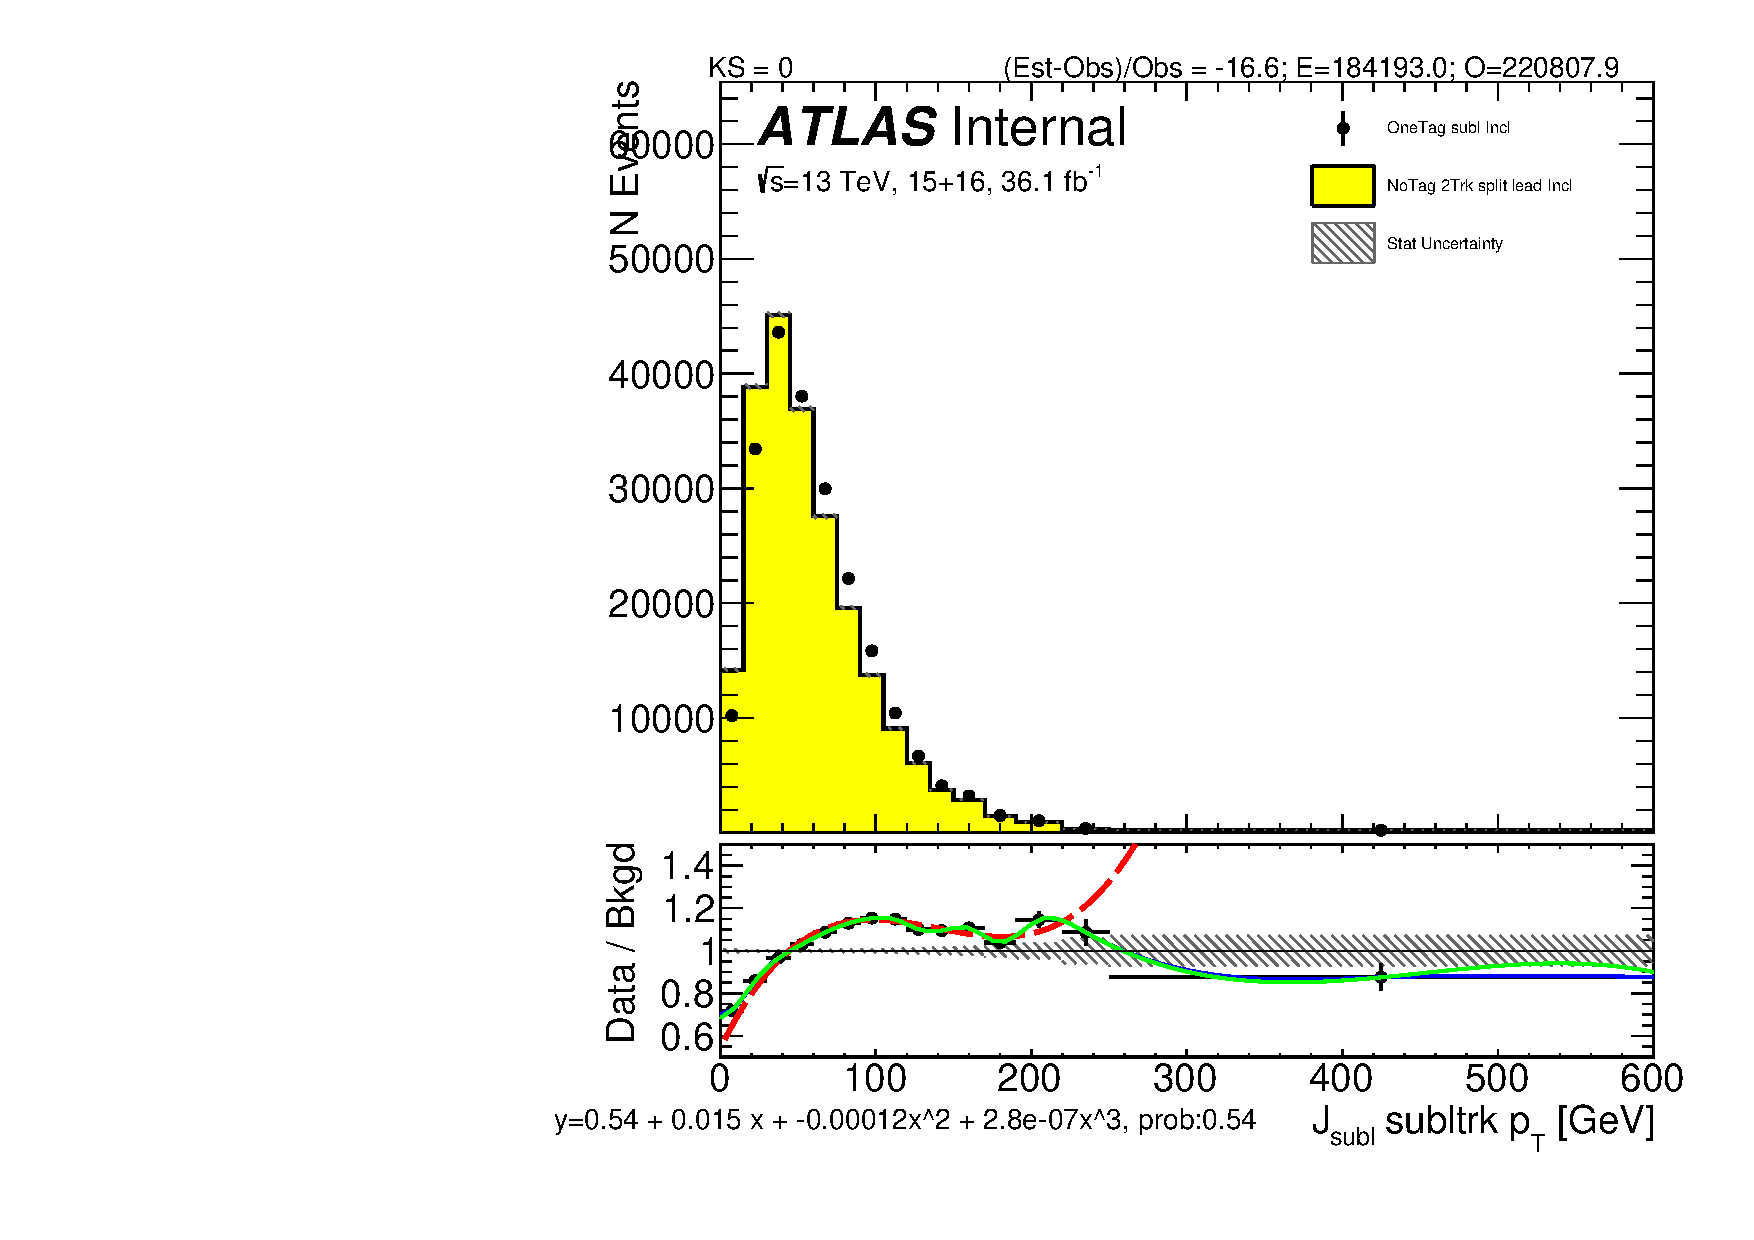
\includegraphics[width=0.32\textwidth,angle=-90]{figures/boosted/Reweight/Fits/Moriond_NoTag_2Trk_split_lead_Incl_sublHCand_trk1_Pt.pdf} \\
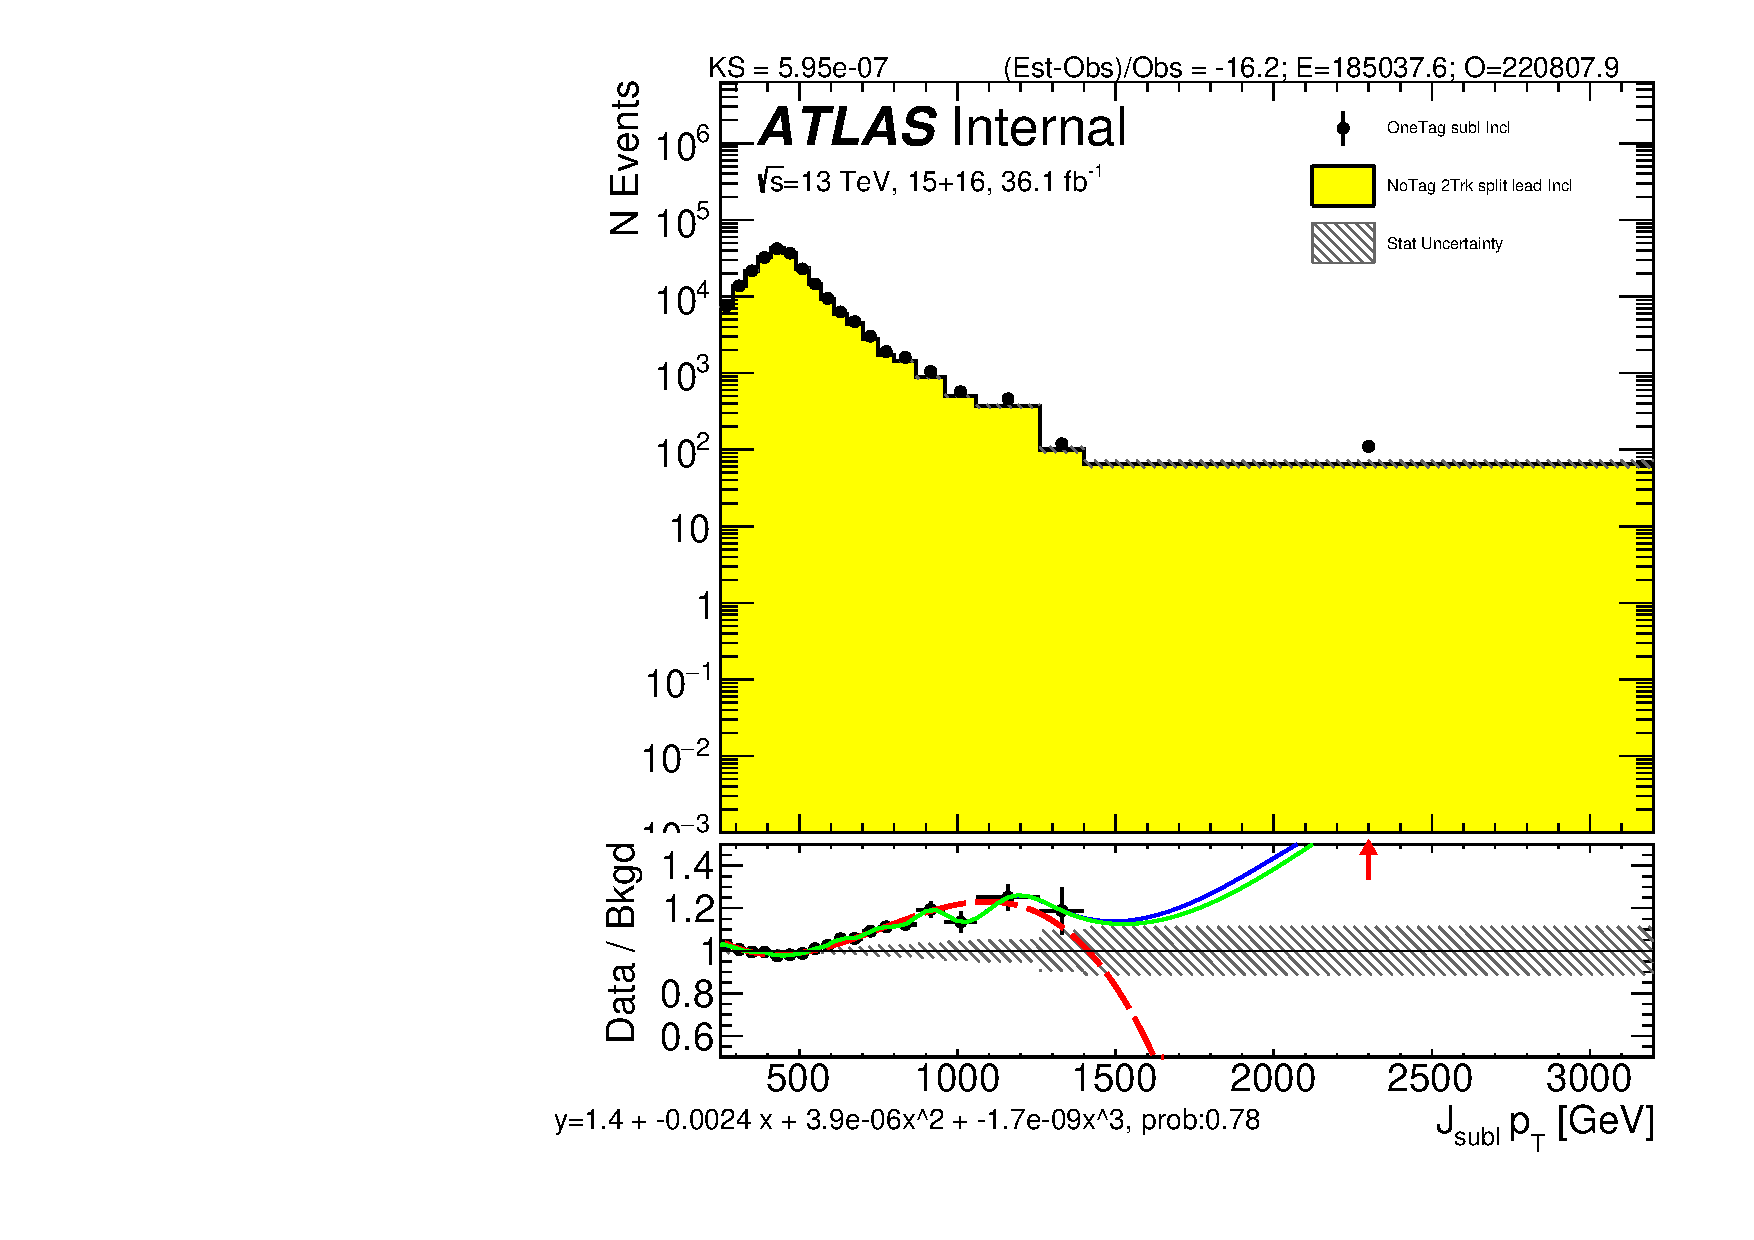
\includegraphics[width=0.32\textwidth,angle=-90]{figures/boosted/Reweight/Fits/Moriond_bkg_0_NoTag_2Trk_split_lead_Incl_sublHCand_Pt_m_1.pdf}
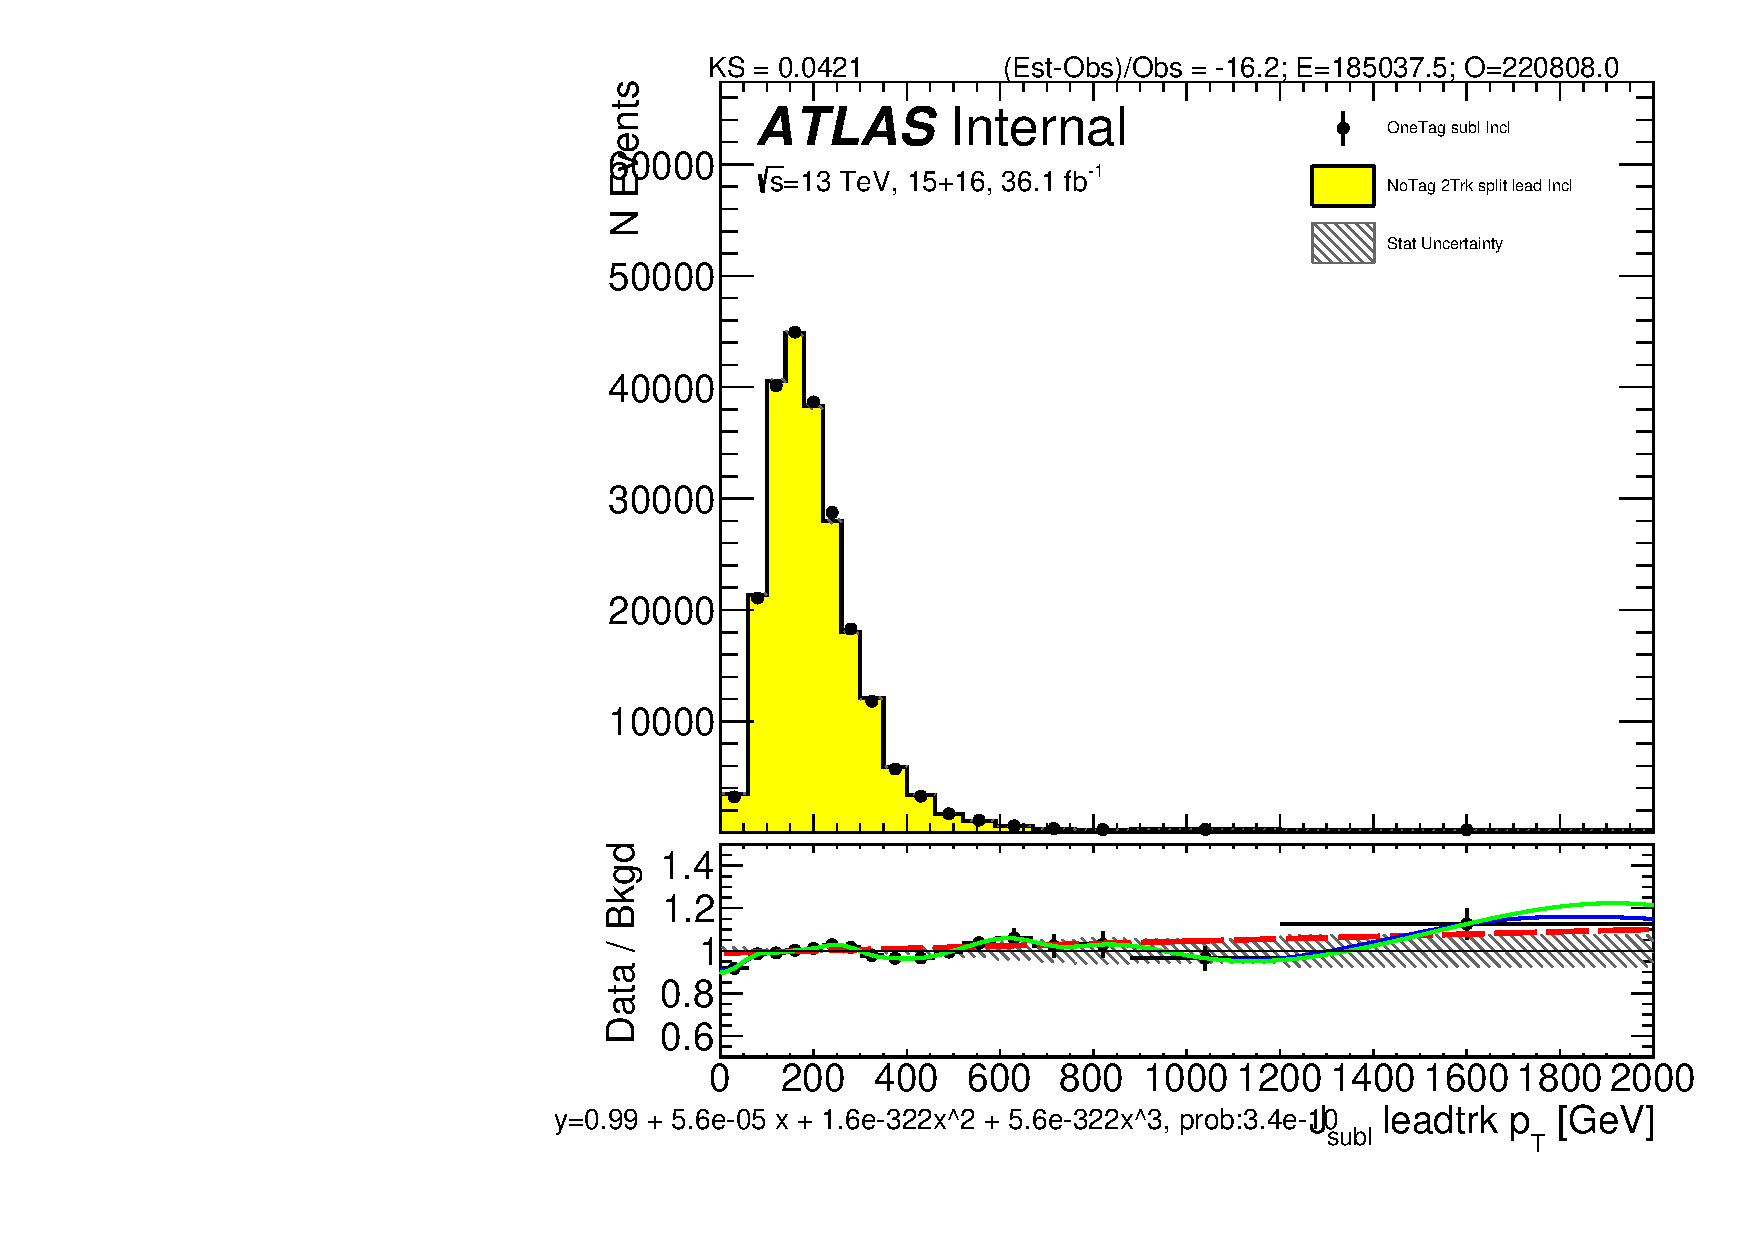
\includegraphics[width=0.32\textwidth,angle=-90]{figures/boosted/Reweight/Fits/Moriond_bkg_0_NoTag_2Trk_split_lead_Incl_sublHCand_trk0_Pt.pdf}
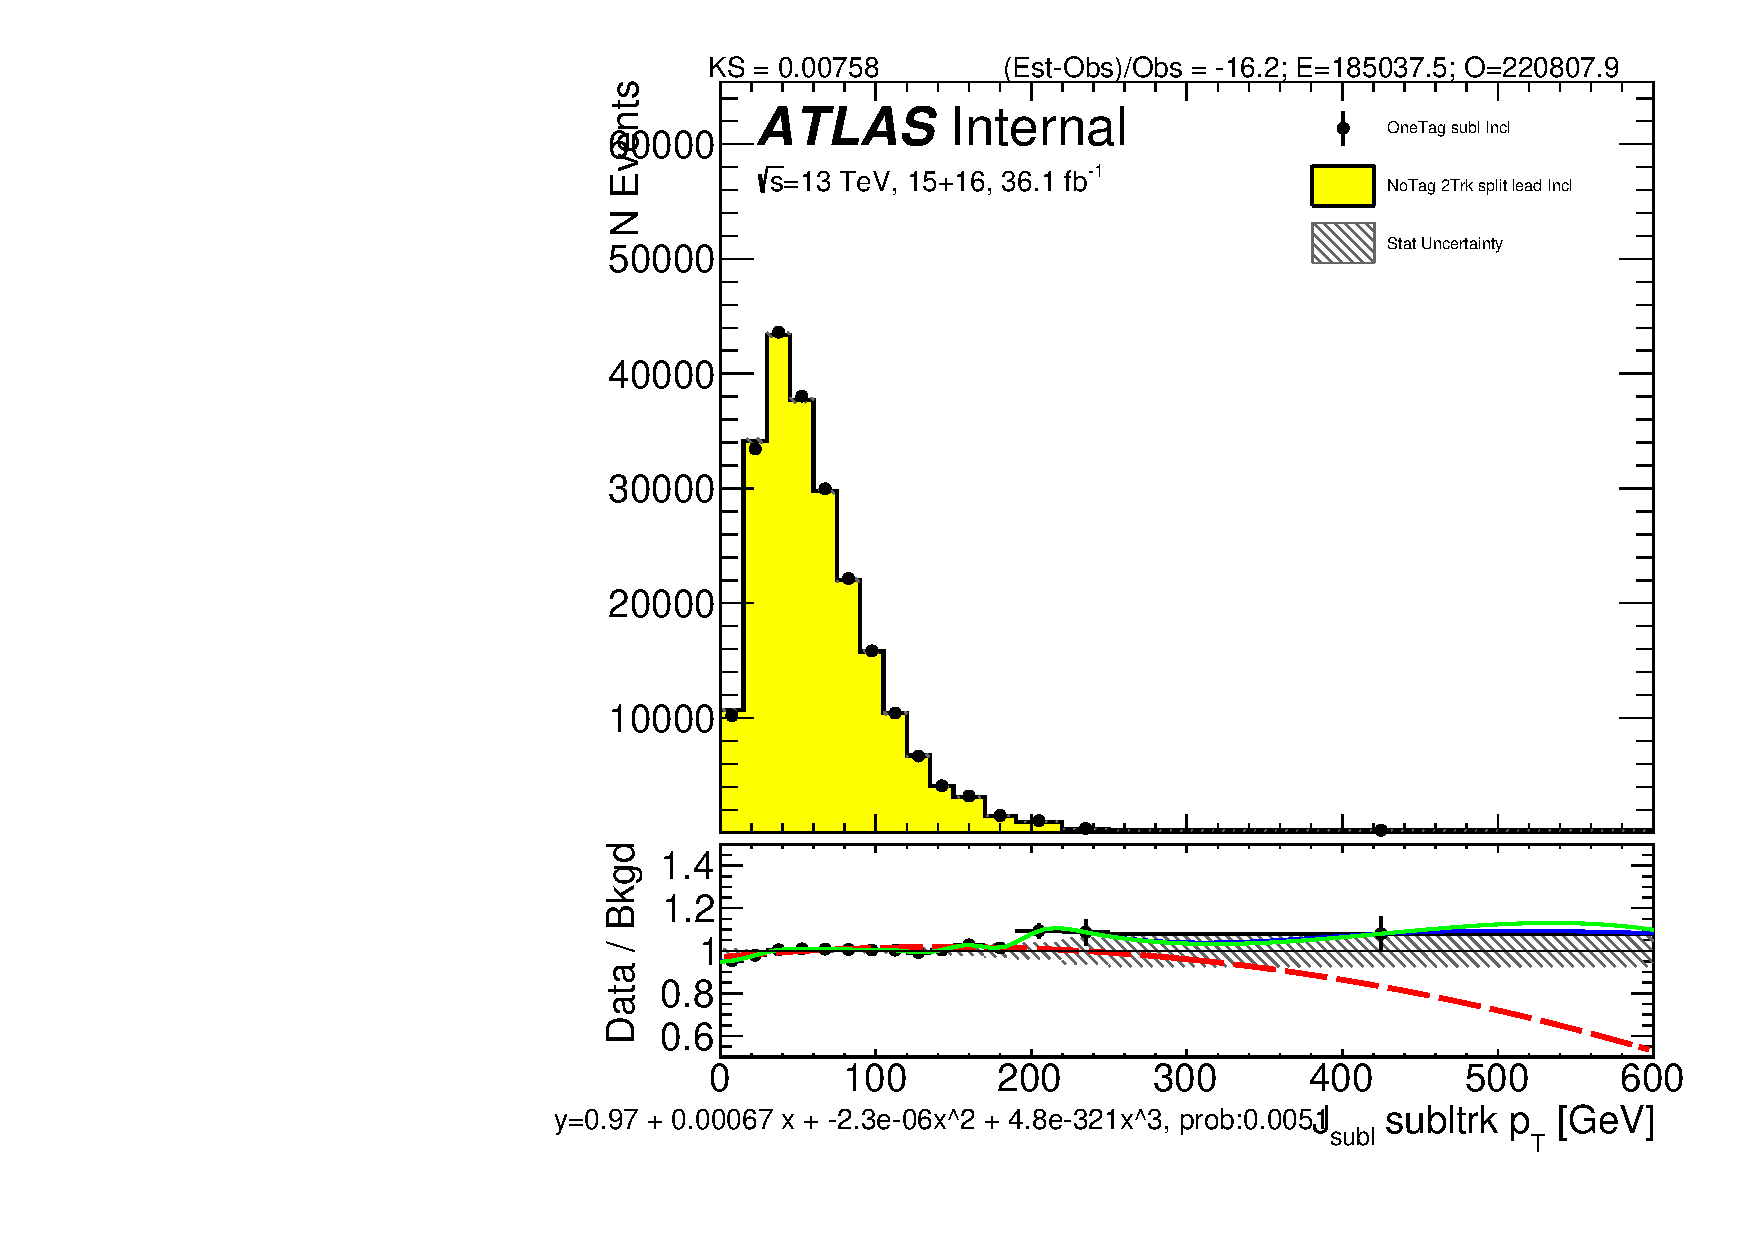
\includegraphics[width=0.32\textwidth,angle=-90]{figures/boosted/Reweight/Fits/Moriond_bkg_0_NoTag_2Trk_split_lead_Incl_sublHCand_trk1_Pt.pdf} \\
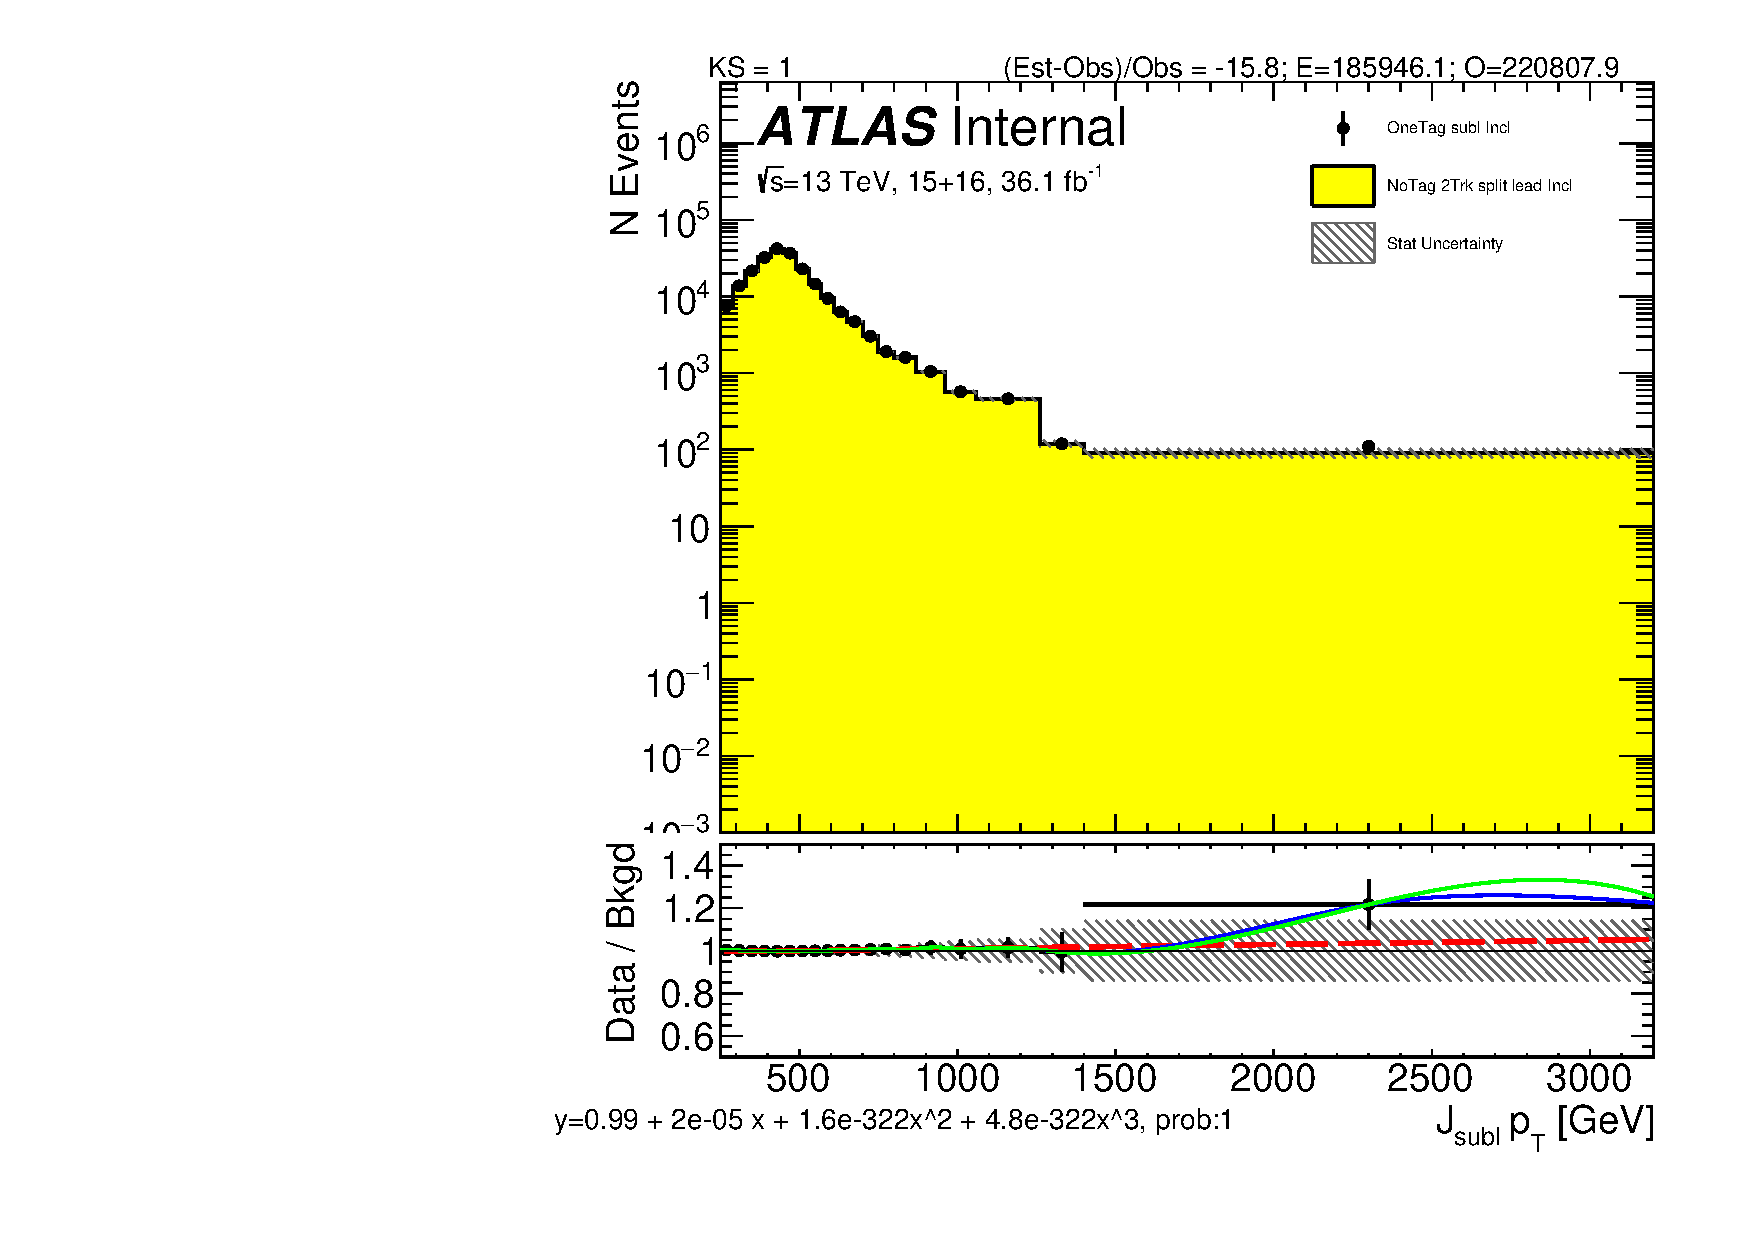
\includegraphics[width=0.32\textwidth,angle=-90]{figures/boosted/Reweight/Fits/Moriond_bkg_3_NoTag_2Trk_split_lead_Incl_sublHCand_Pt_m_1.pdf}
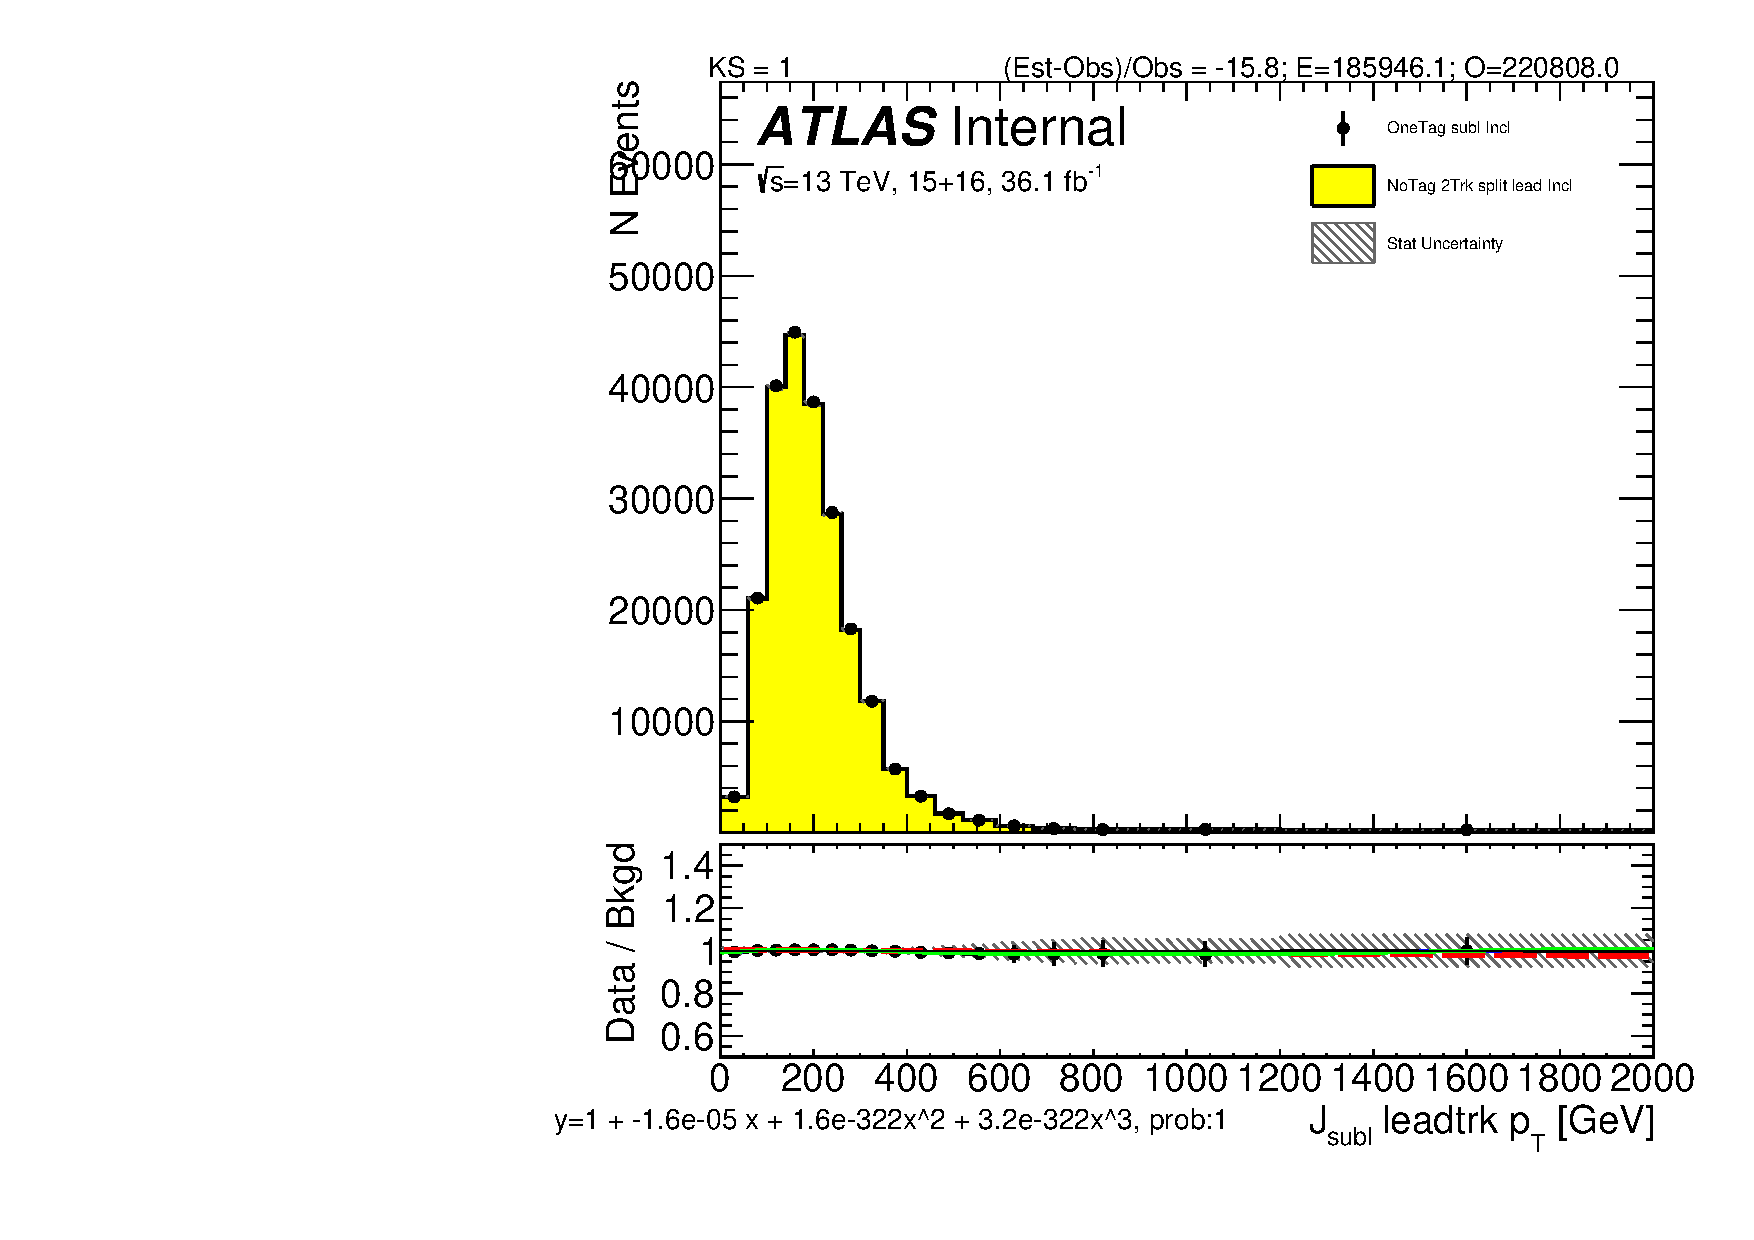
\includegraphics[width=0.32\textwidth,angle=-90]{figures/boosted/Reweight/Fits/Moriond_bkg_3_NoTag_2Trk_split_lead_Incl_sublHCand_trk0_Pt.pdf}
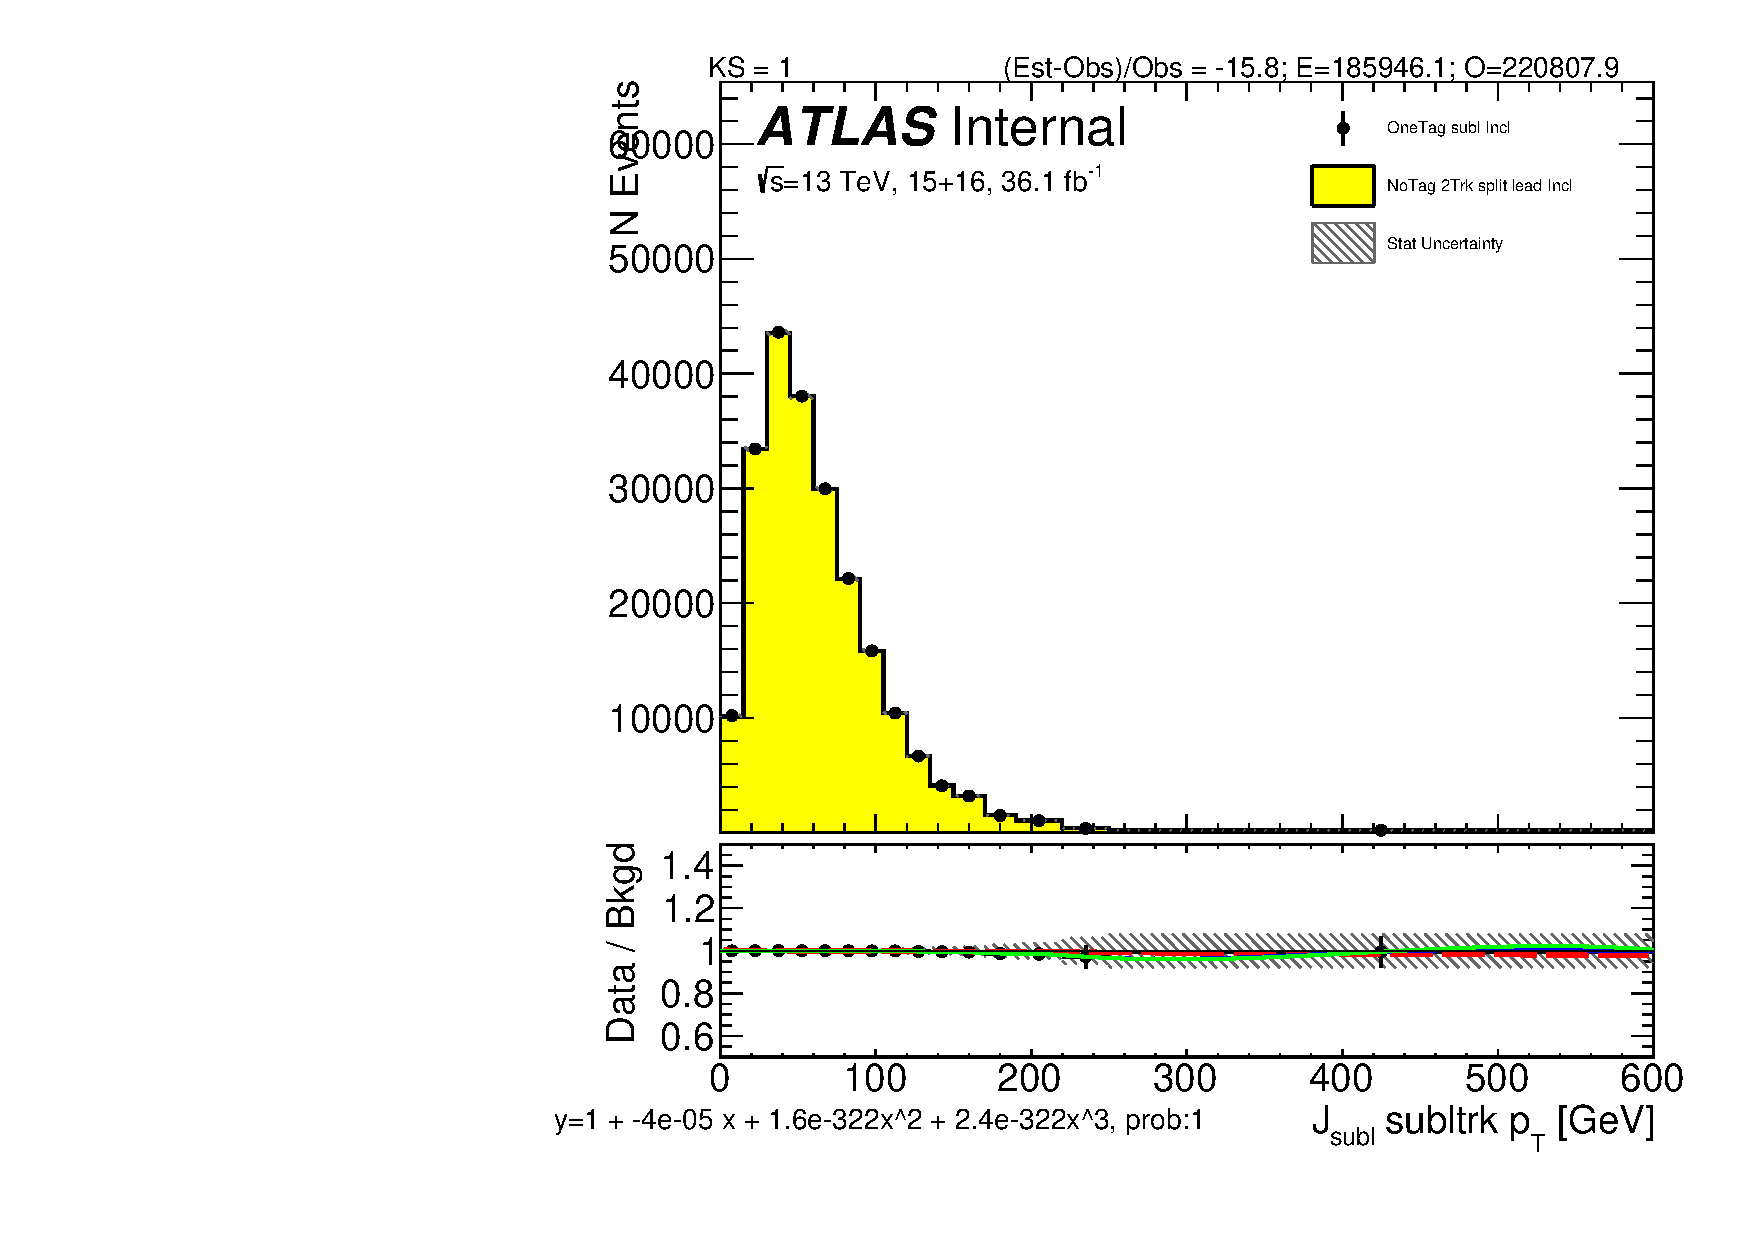
\includegraphics[width=0.32\textwidth,angle=-90]{figures/boosted/Reweight/Fits/Moriond_bkg_3_NoTag_2Trk_split_lead_Incl_sublHCand_trk1_Pt.pdf} \\
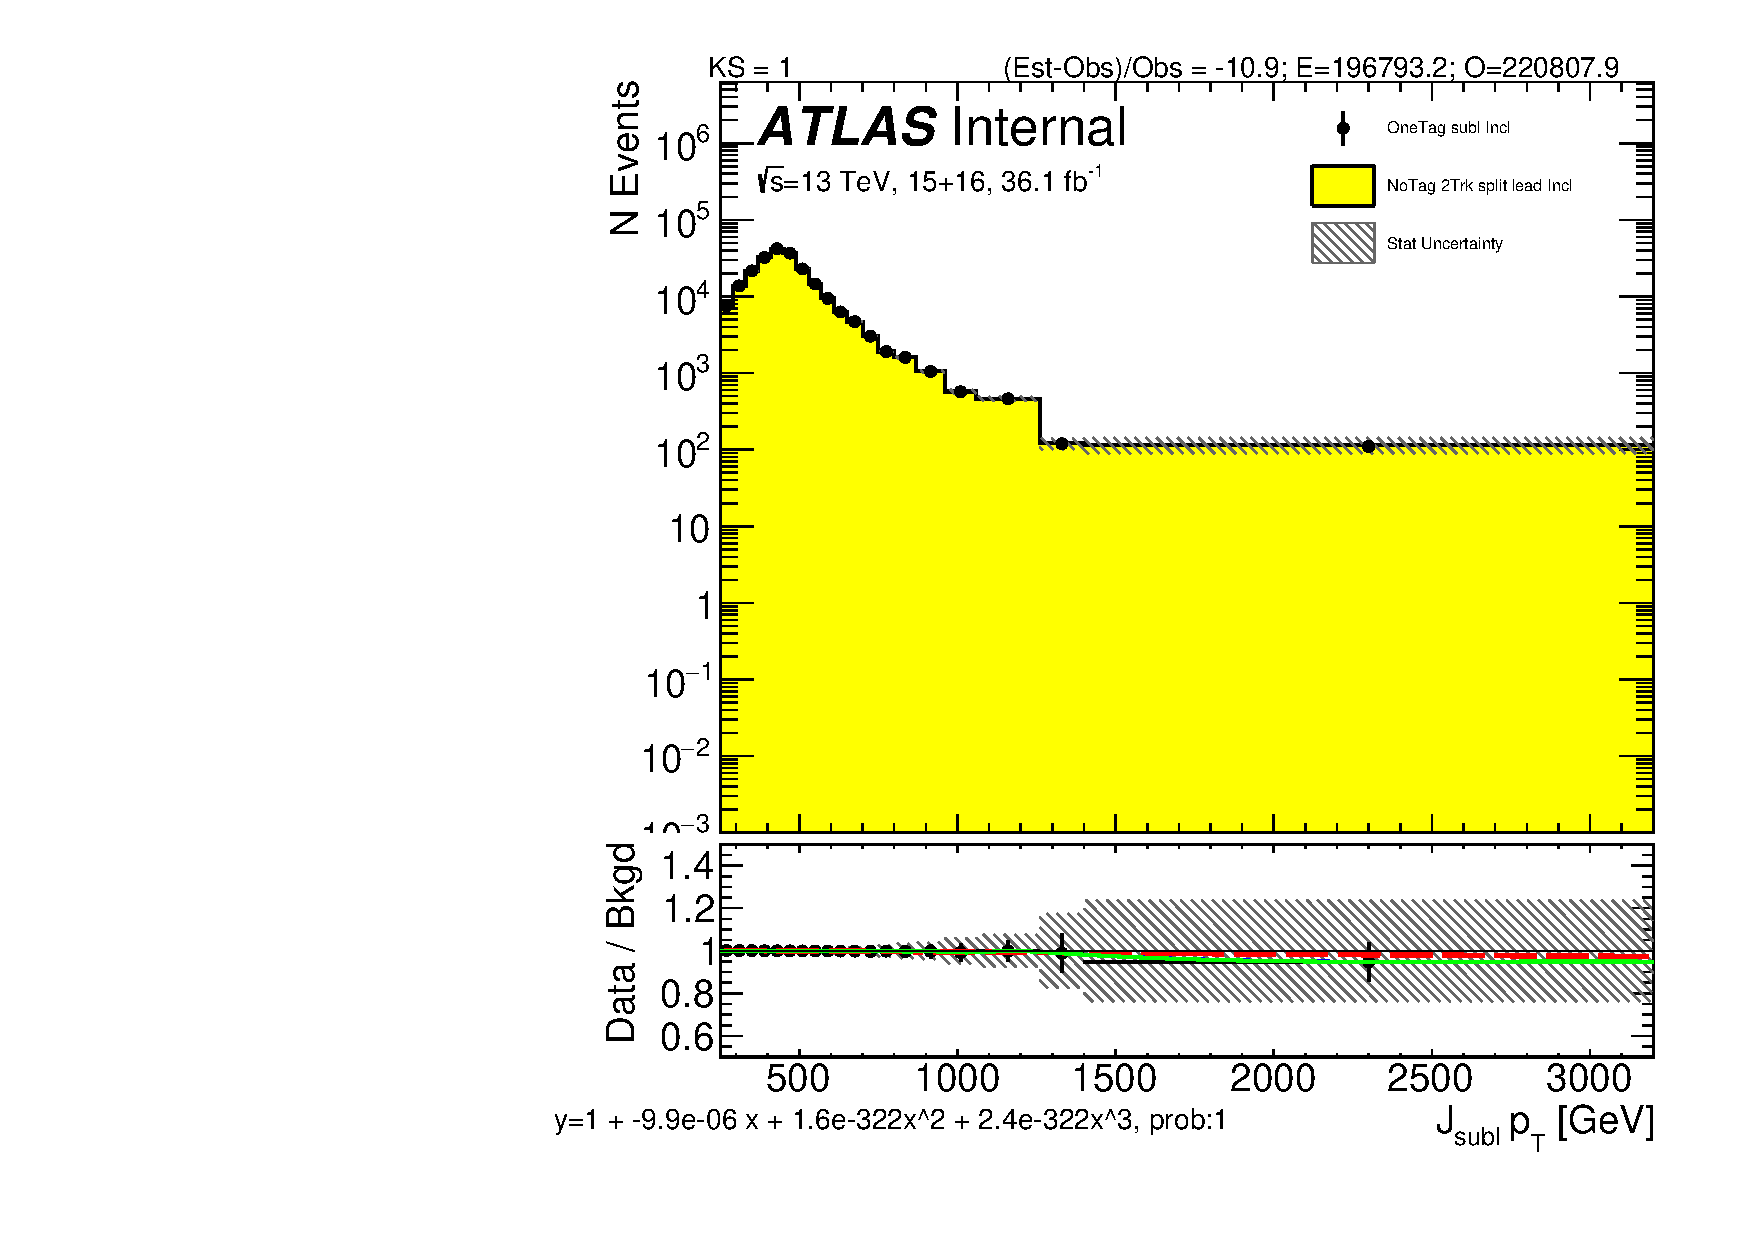
\includegraphics[width=0.32\textwidth,angle=-90]{figures/boosted/Reweight/Fits/Moriond_bkg_9_NoTag_2Trk_split_lead_Incl_sublHCand_Pt_m_1.pdf}
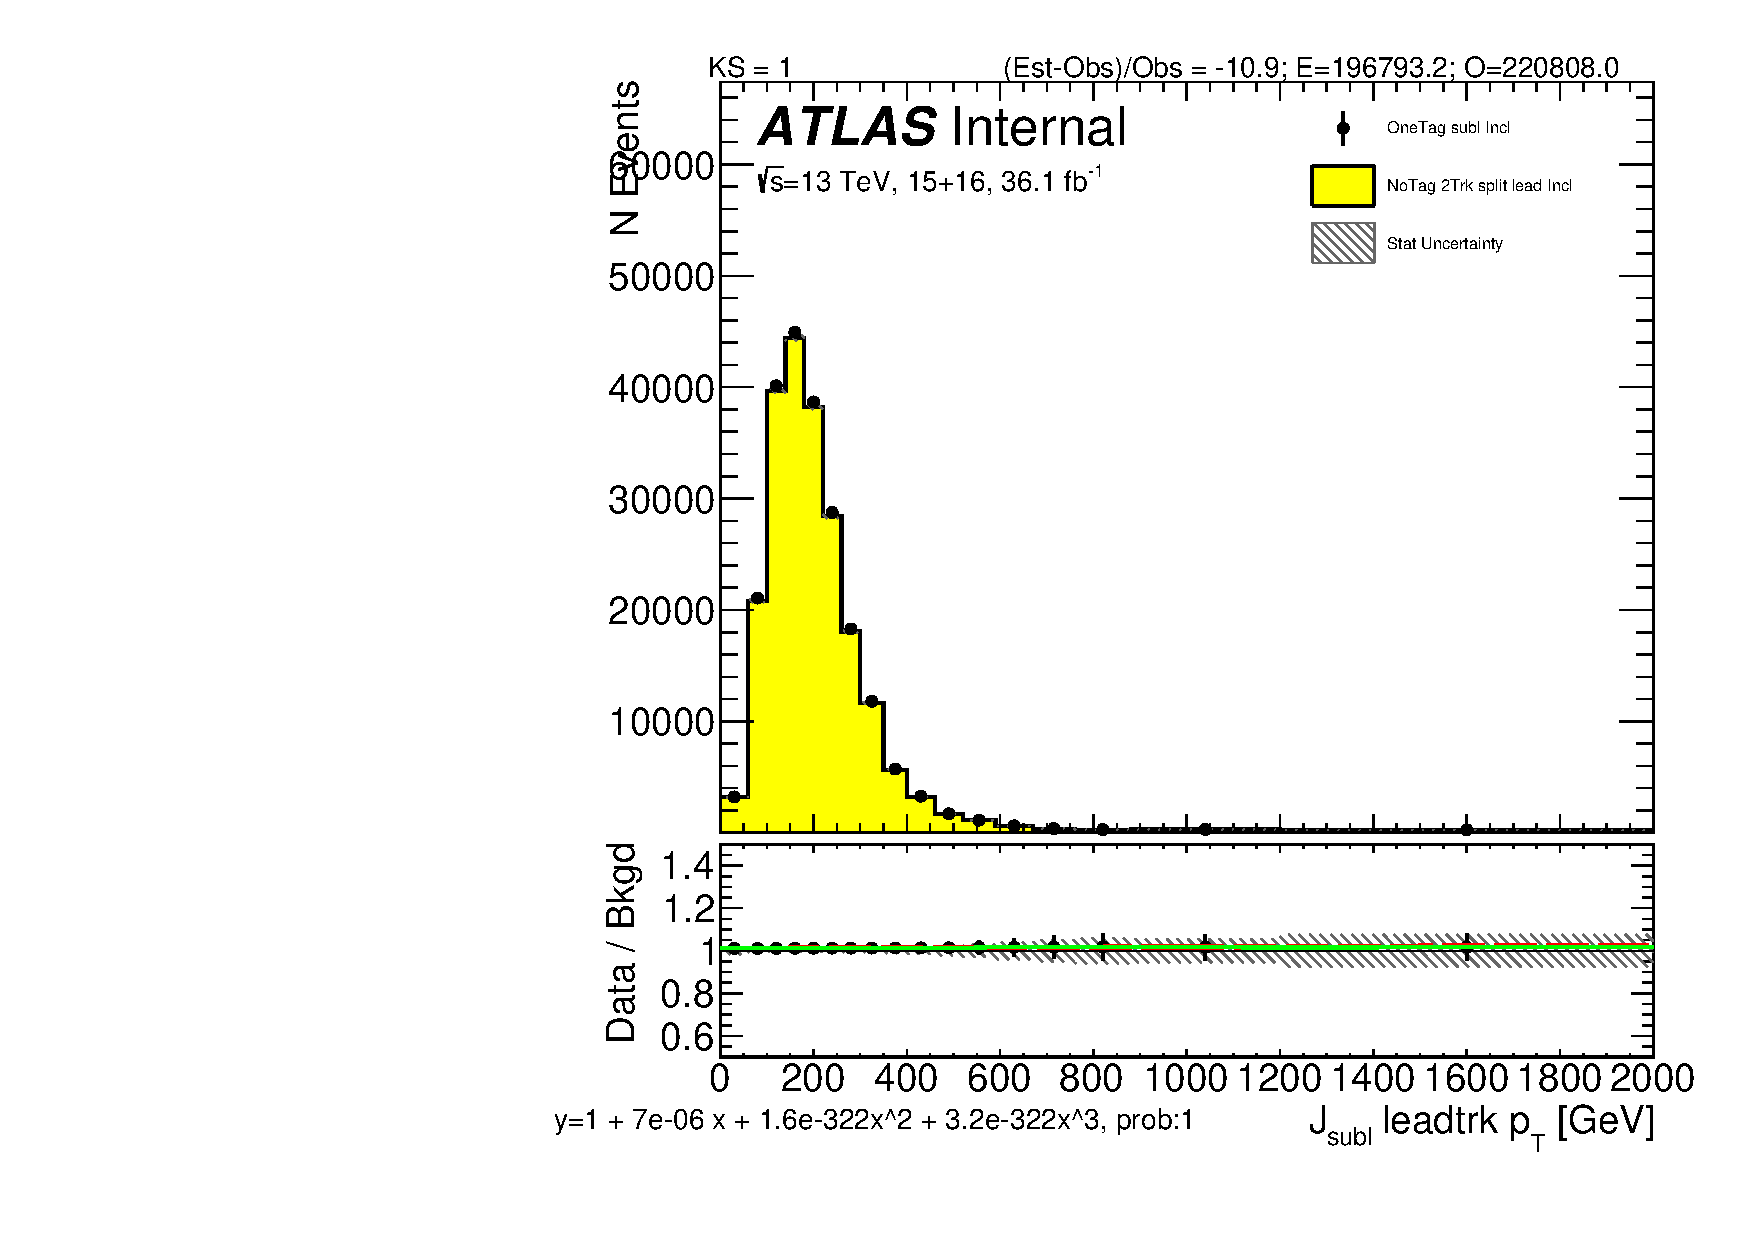
\includegraphics[width=0.32\textwidth,angle=-90]{figures/boosted/Reweight/Fits/Moriond_bkg_9_NoTag_2Trk_split_lead_Incl_sublHCand_trk0_Pt.pdf}
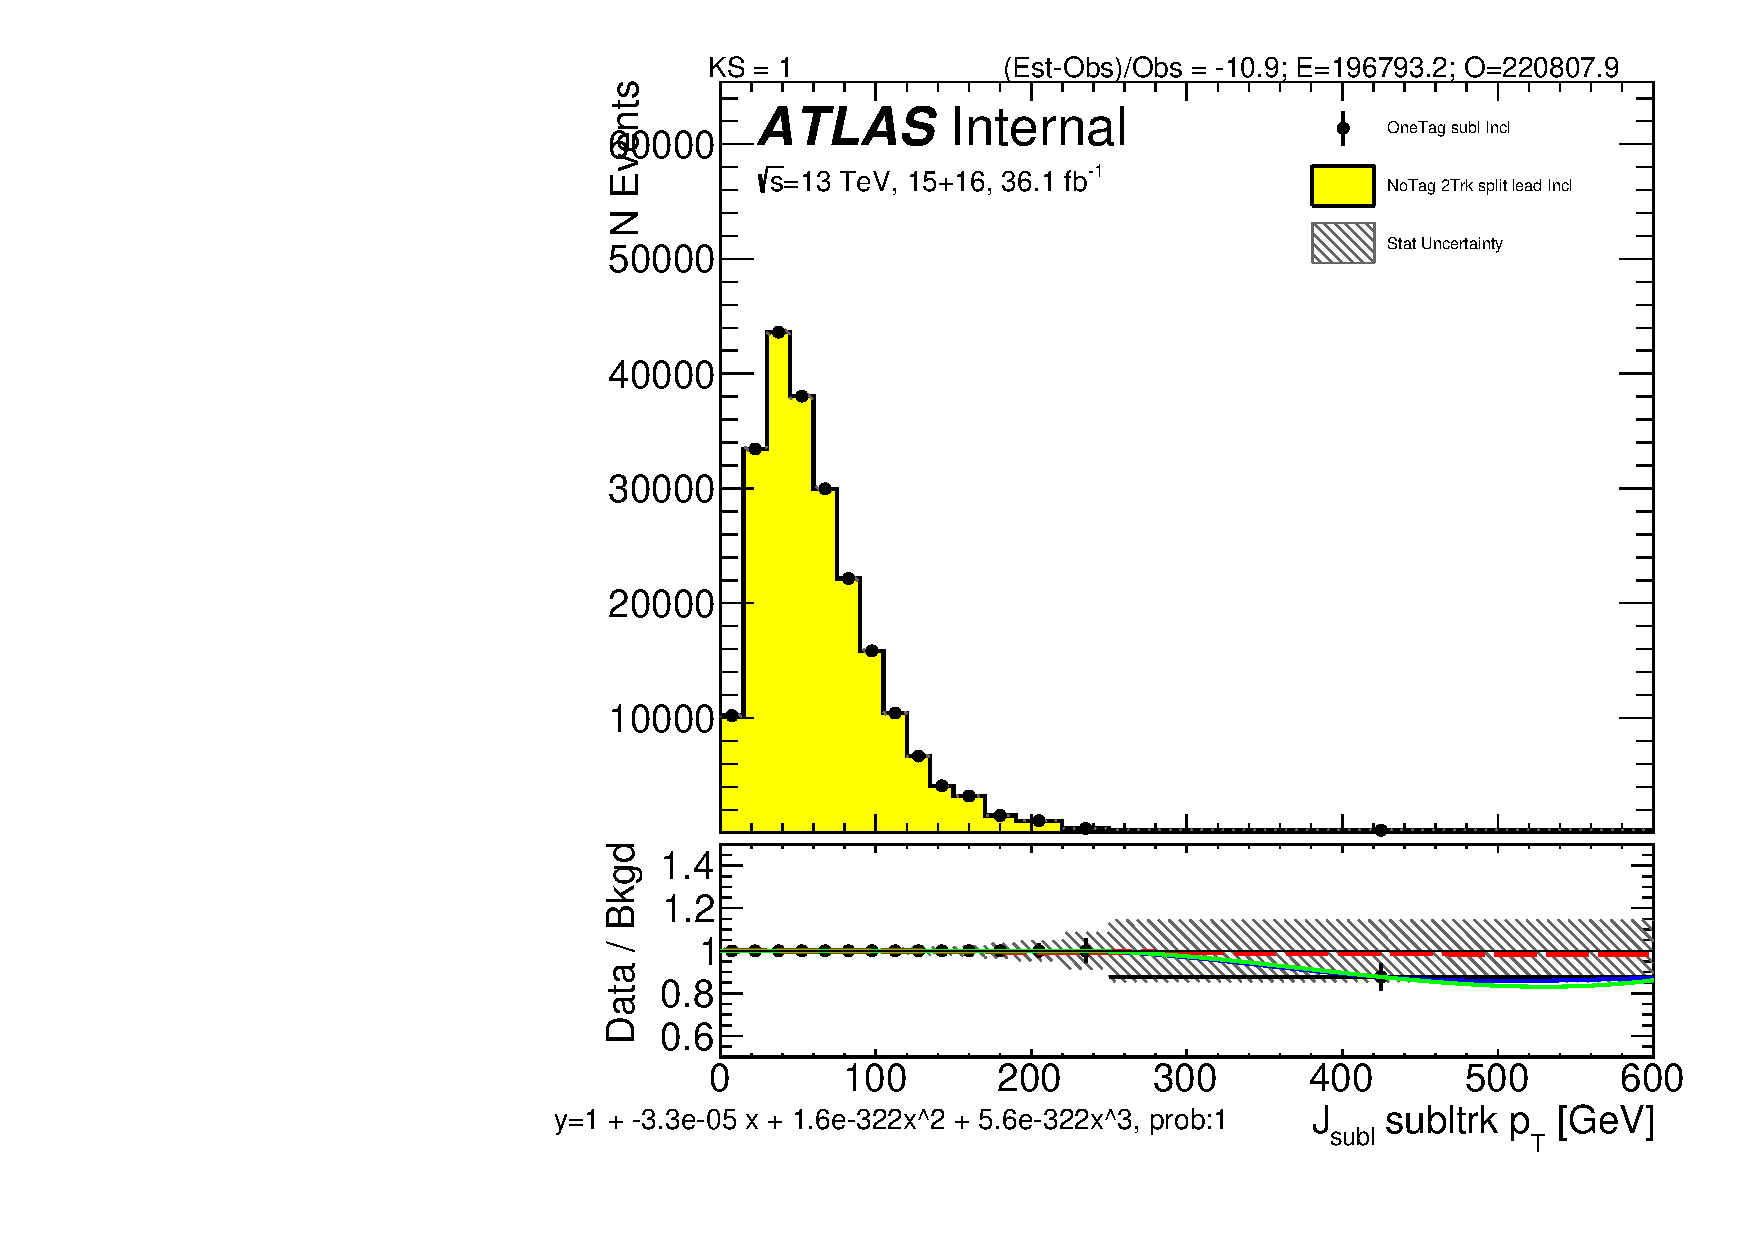
\includegraphics[width=0.32\textwidth,angle=-90]{figures/boosted/Reweight/Fits/Moriond_bkg_9_NoTag_2Trk_split_lead_Incl_sublHCand_trk1_Pt.pdf} \\
\caption{For $2b$s background estimate: the fits to the ratio of the data in the 1$b$ category, of the sublleading Higgs candidate 1$b$-tagged events's subleading Higgs candidate distributions(black point), over the leading Higgs candidate 1$b$-tagged events's subleading Higgs candidate distributions(yellow). Distributions and fits to the estimated QCD background for large-$R$ jet $p_{T}$ (left),  the large-$R$ jet's leading trackjet $p_T$ (middle), and large-$R$ jet's subleading trackjet $p_T$ (right) are shown.  Figure are shown before reweighting (top row), after the first iteration(second row), after the fourth iteration(third row), and after the last iteration (bottow row). The green line is the spline extrapolation; and the red line is a polynomial fit.}
\label{fig:rw-2bs-lead}
\end{center}
\end{figure*}

\begin{figure*}[htbp!]
\begin{center}
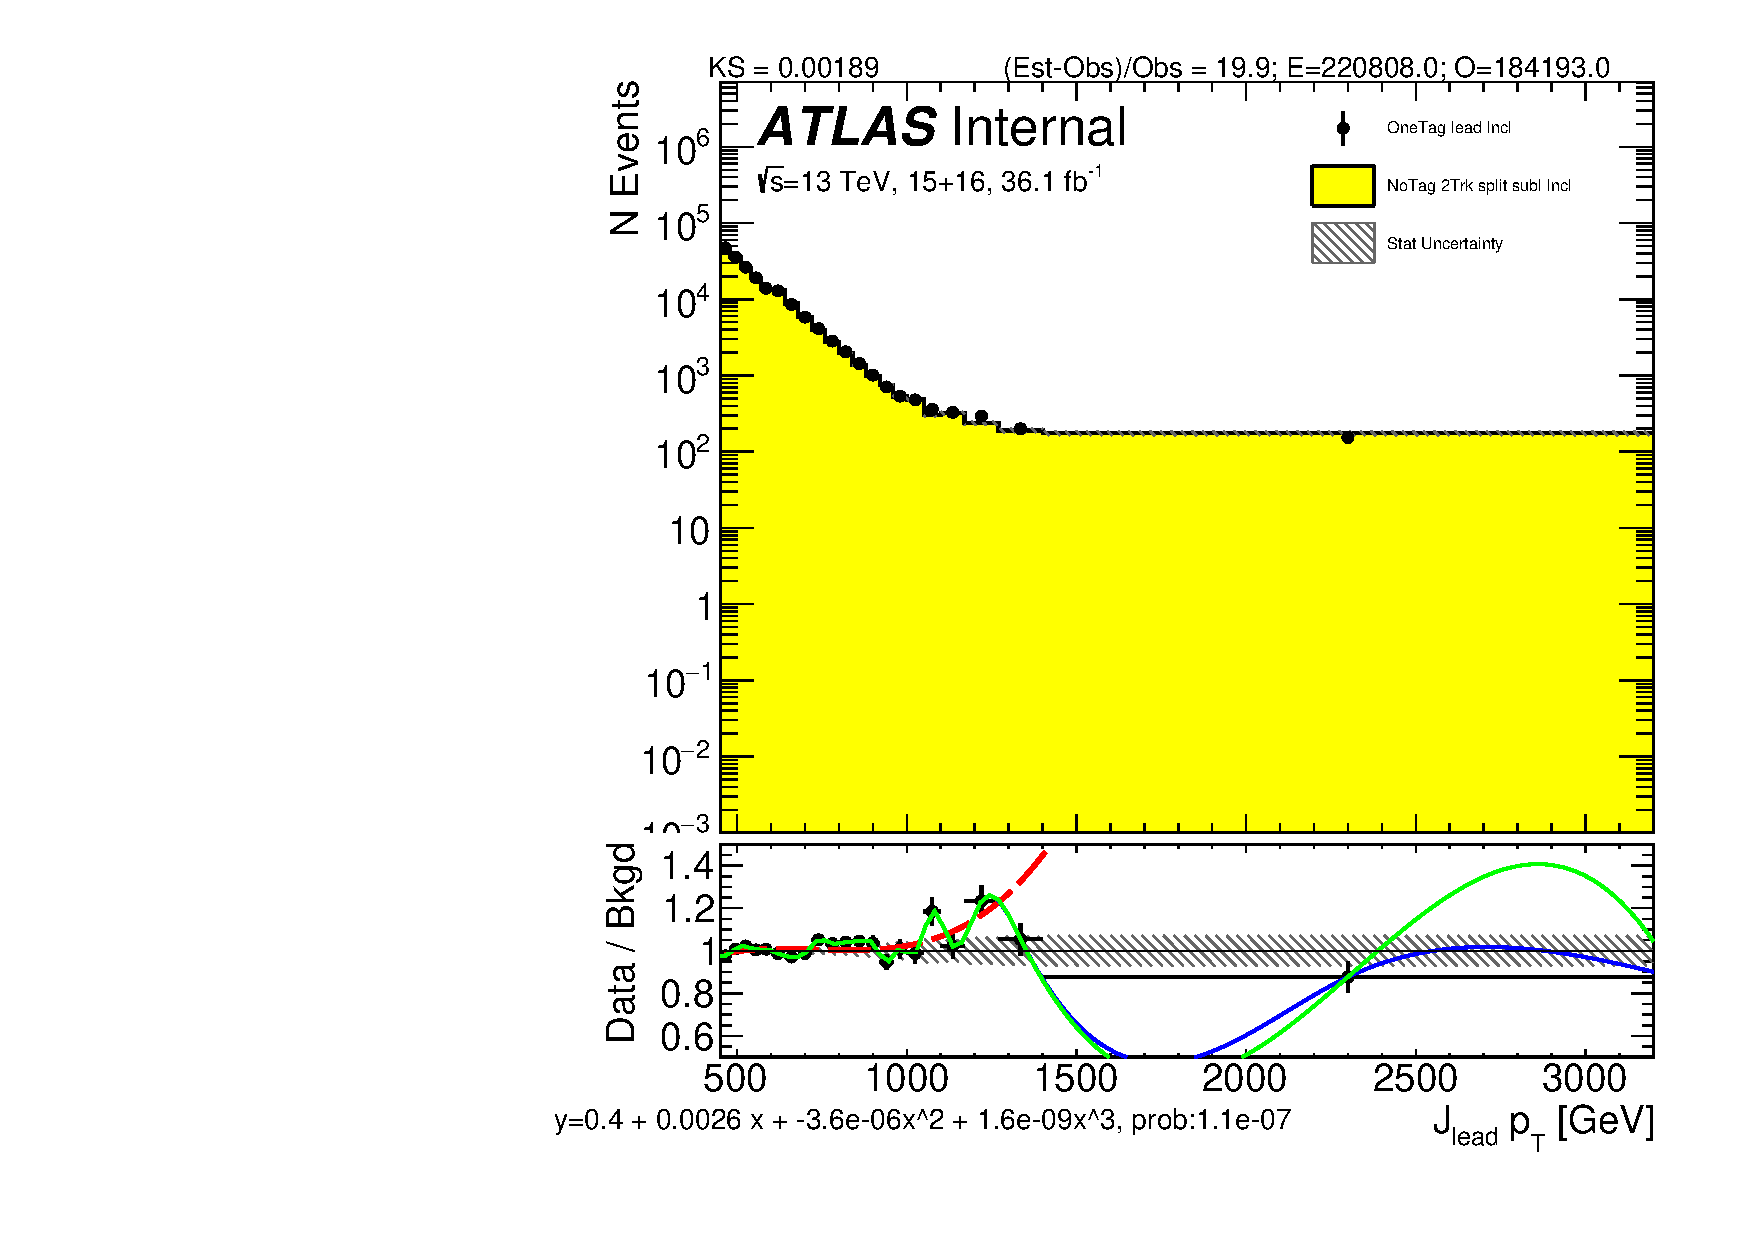
\includegraphics[width=0.32\textwidth,angle=-90]{figures/boosted/Reweight/Fits/Moriond_NoTag_2Trk_split_subl_Incl_leadHCand_Pt_m_1.pdf}
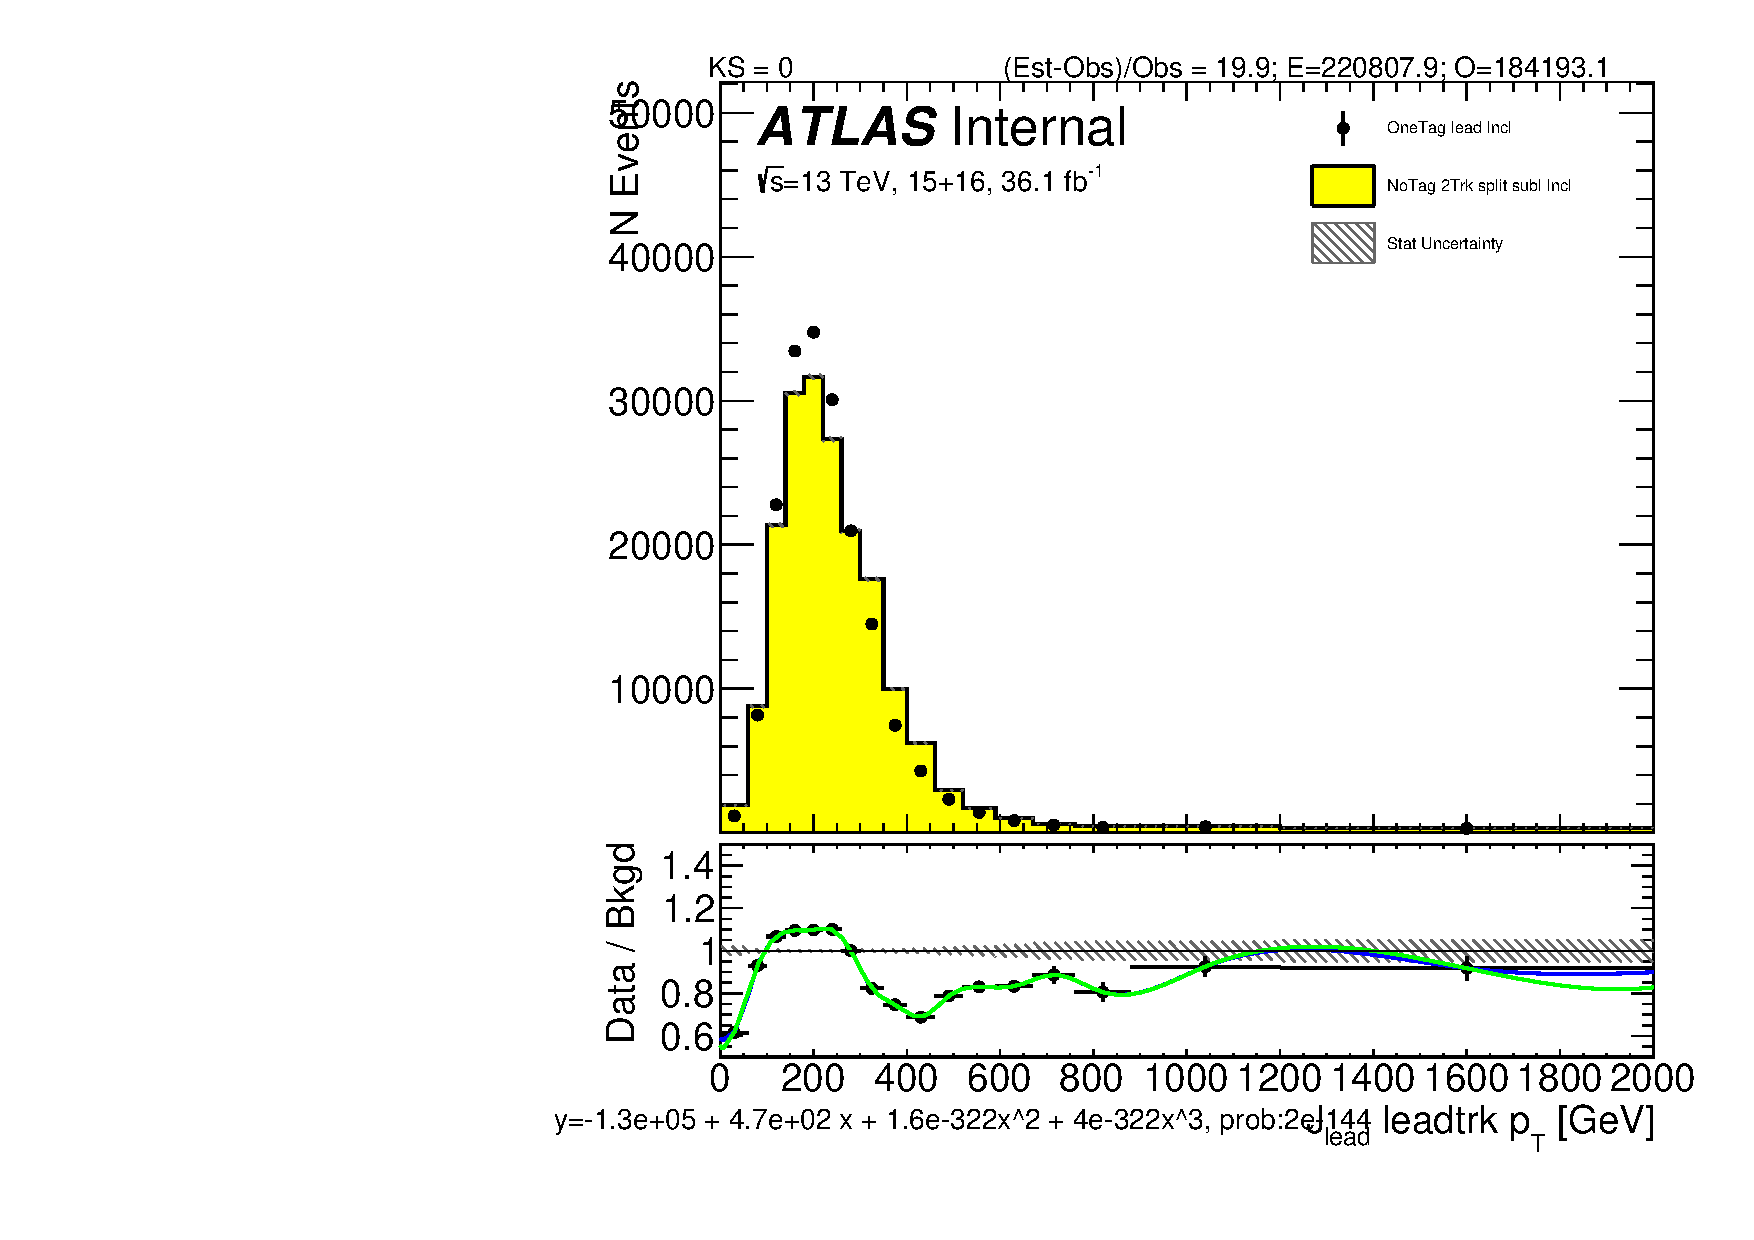
\includegraphics[width=0.32\textwidth,angle=-90]{figures/boosted/Reweight/Fits/Moriond_NoTag_2Trk_split_subl_Incl_leadHCand_trk0_Pt.pdf}
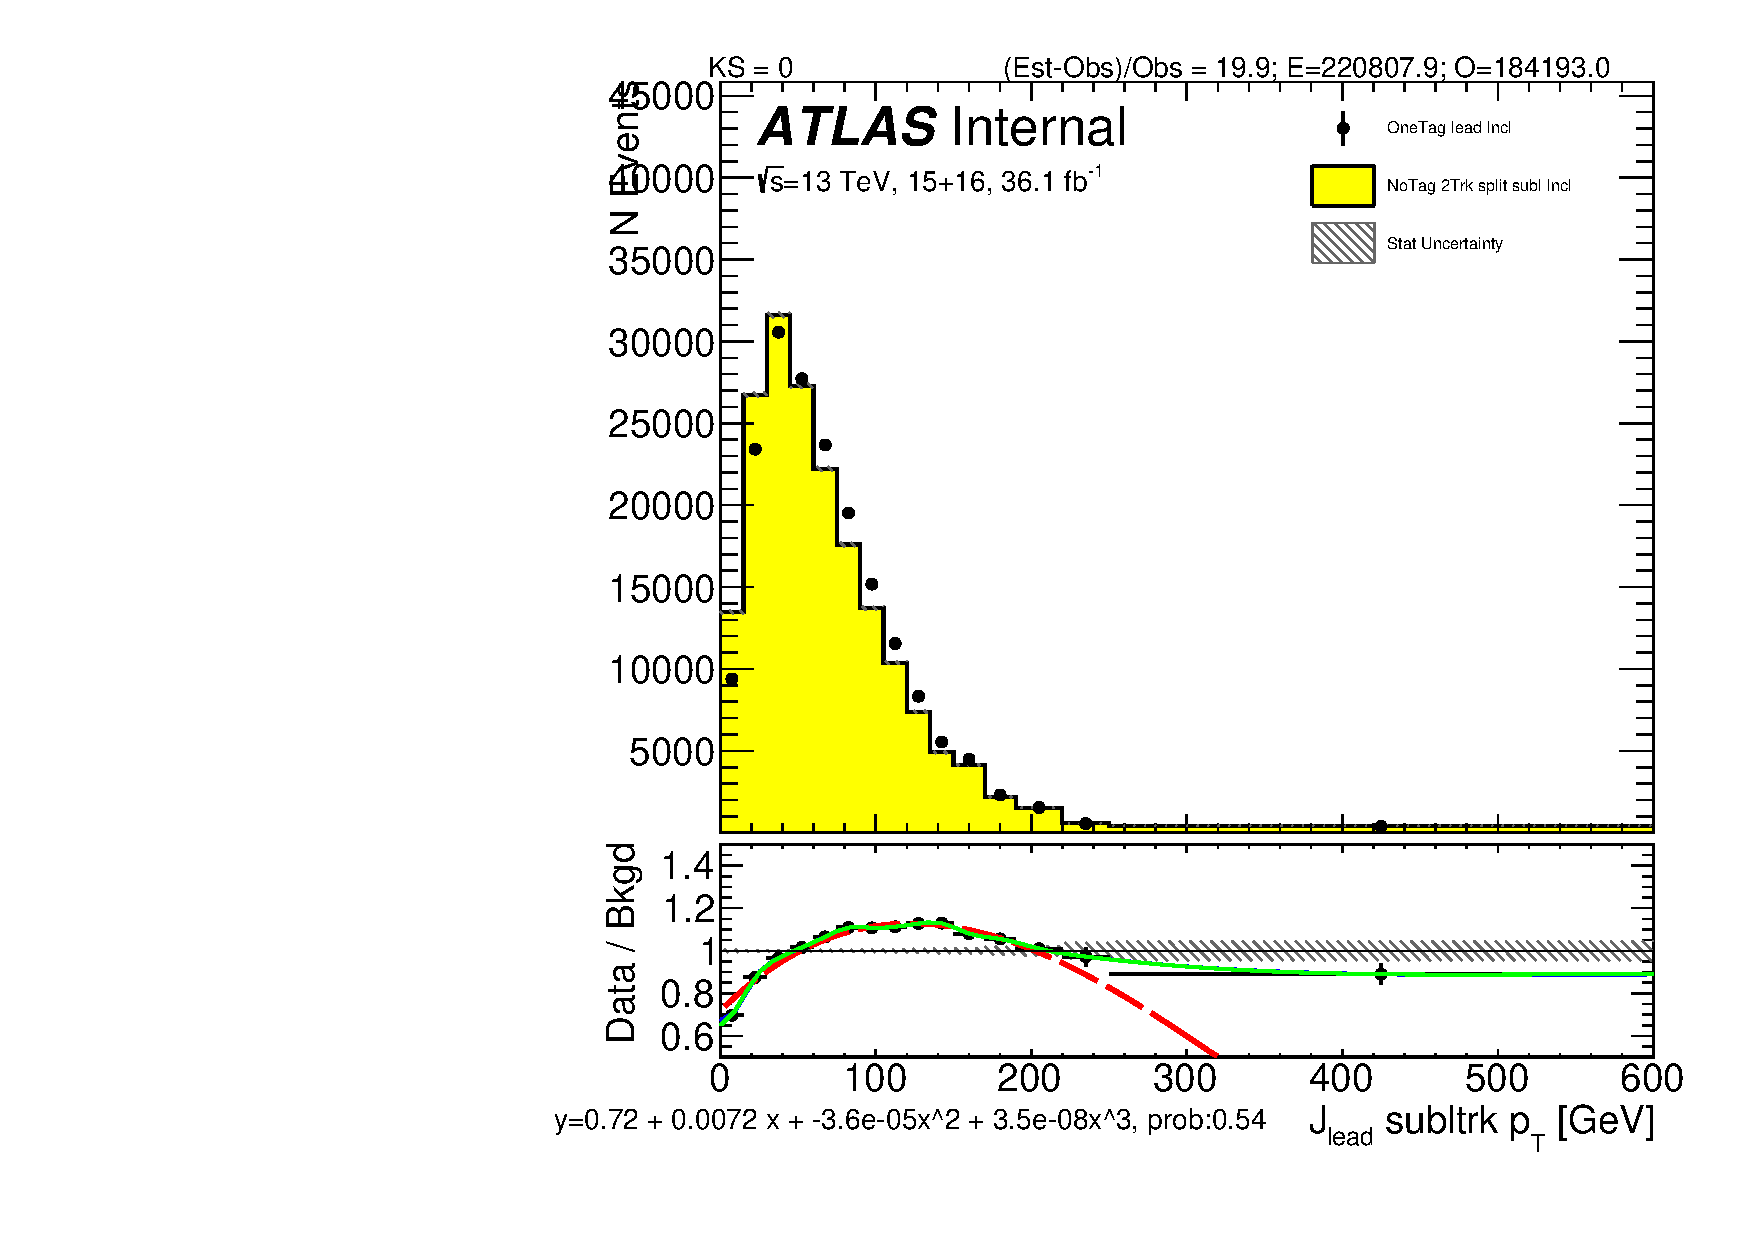
\includegraphics[width=0.32\textwidth,angle=-90]{figures/boosted/Reweight/Fits/Moriond_NoTag_2Trk_split_subl_Incl_leadHCand_trk1_Pt.pdf} \\
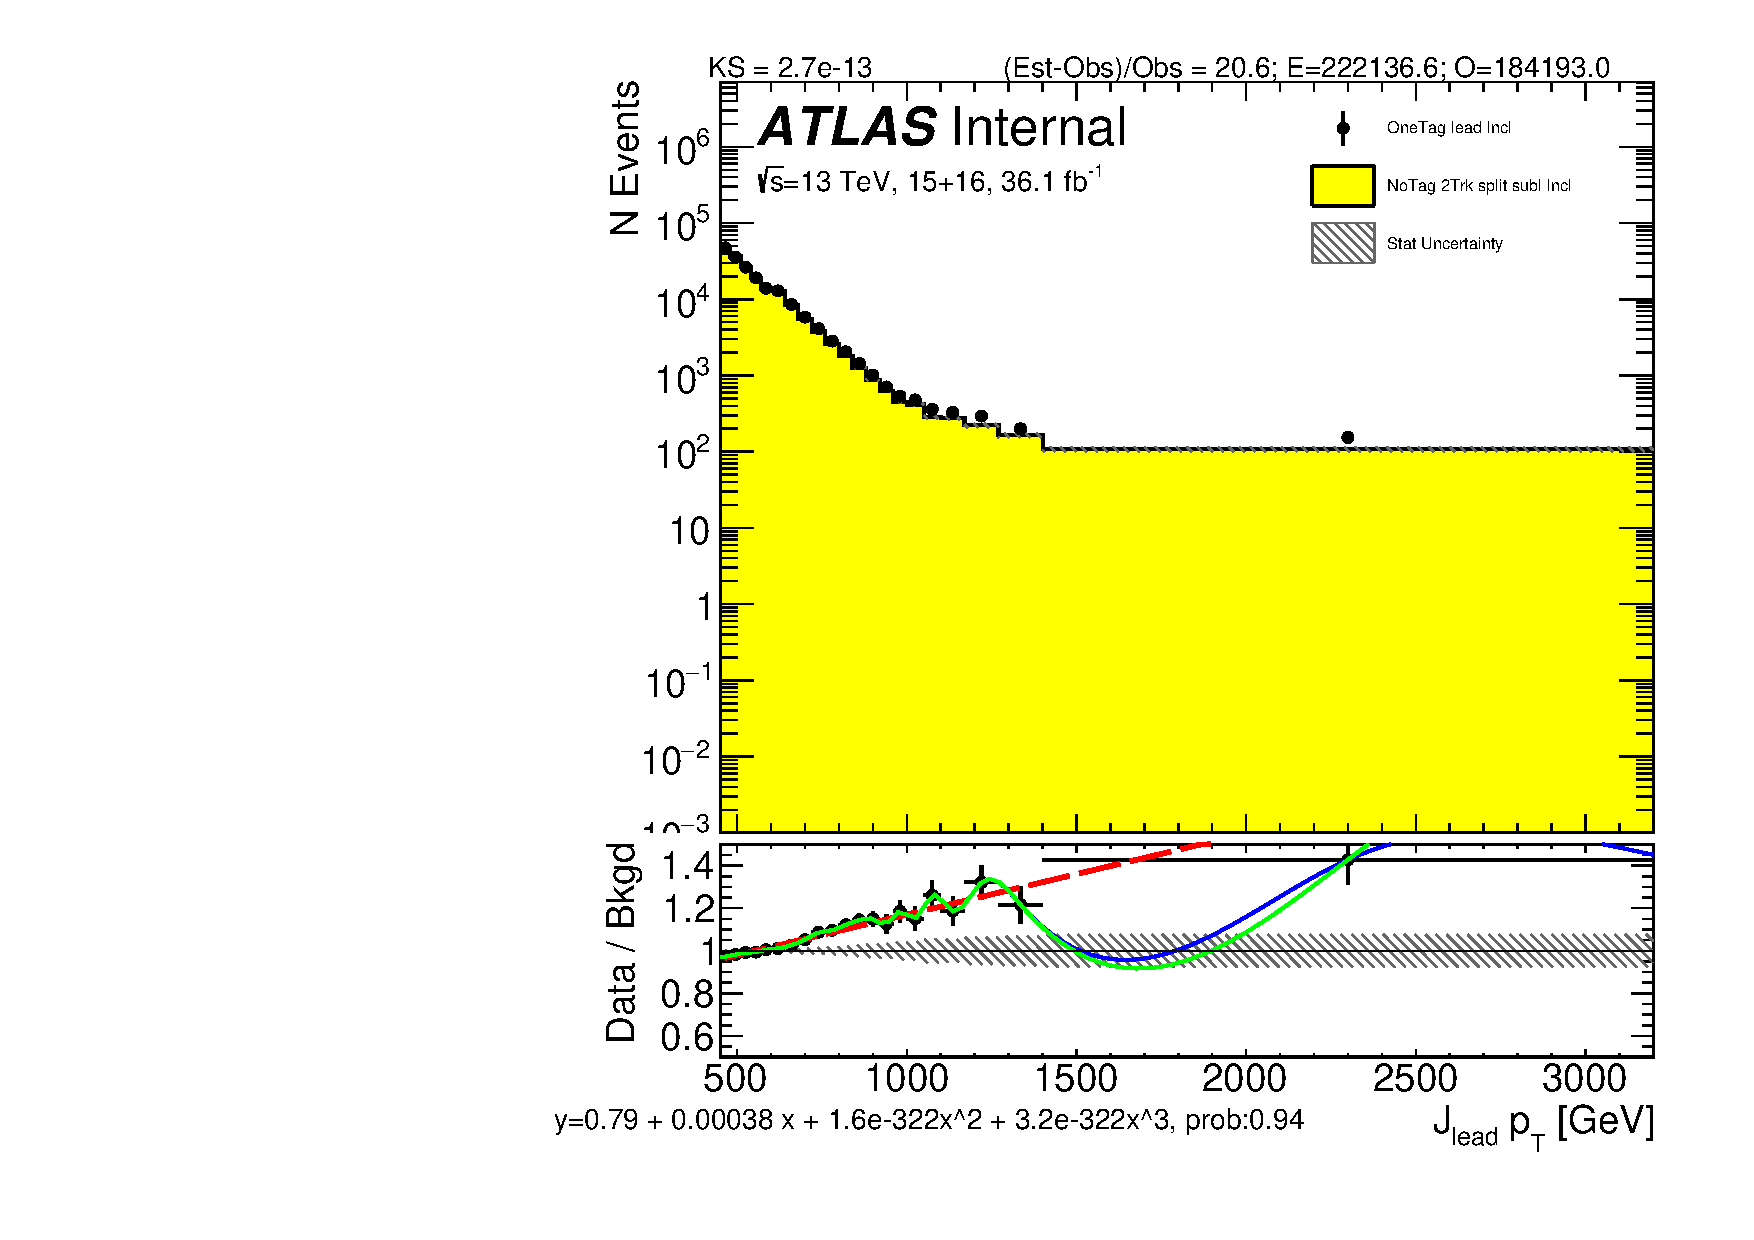
\includegraphics[width=0.32\textwidth,angle=-90]{figures/boosted/Reweight/Fits/Moriond_bkg_0_NoTag_2Trk_split_subl_Incl_leadHCand_Pt_m_1.pdf}
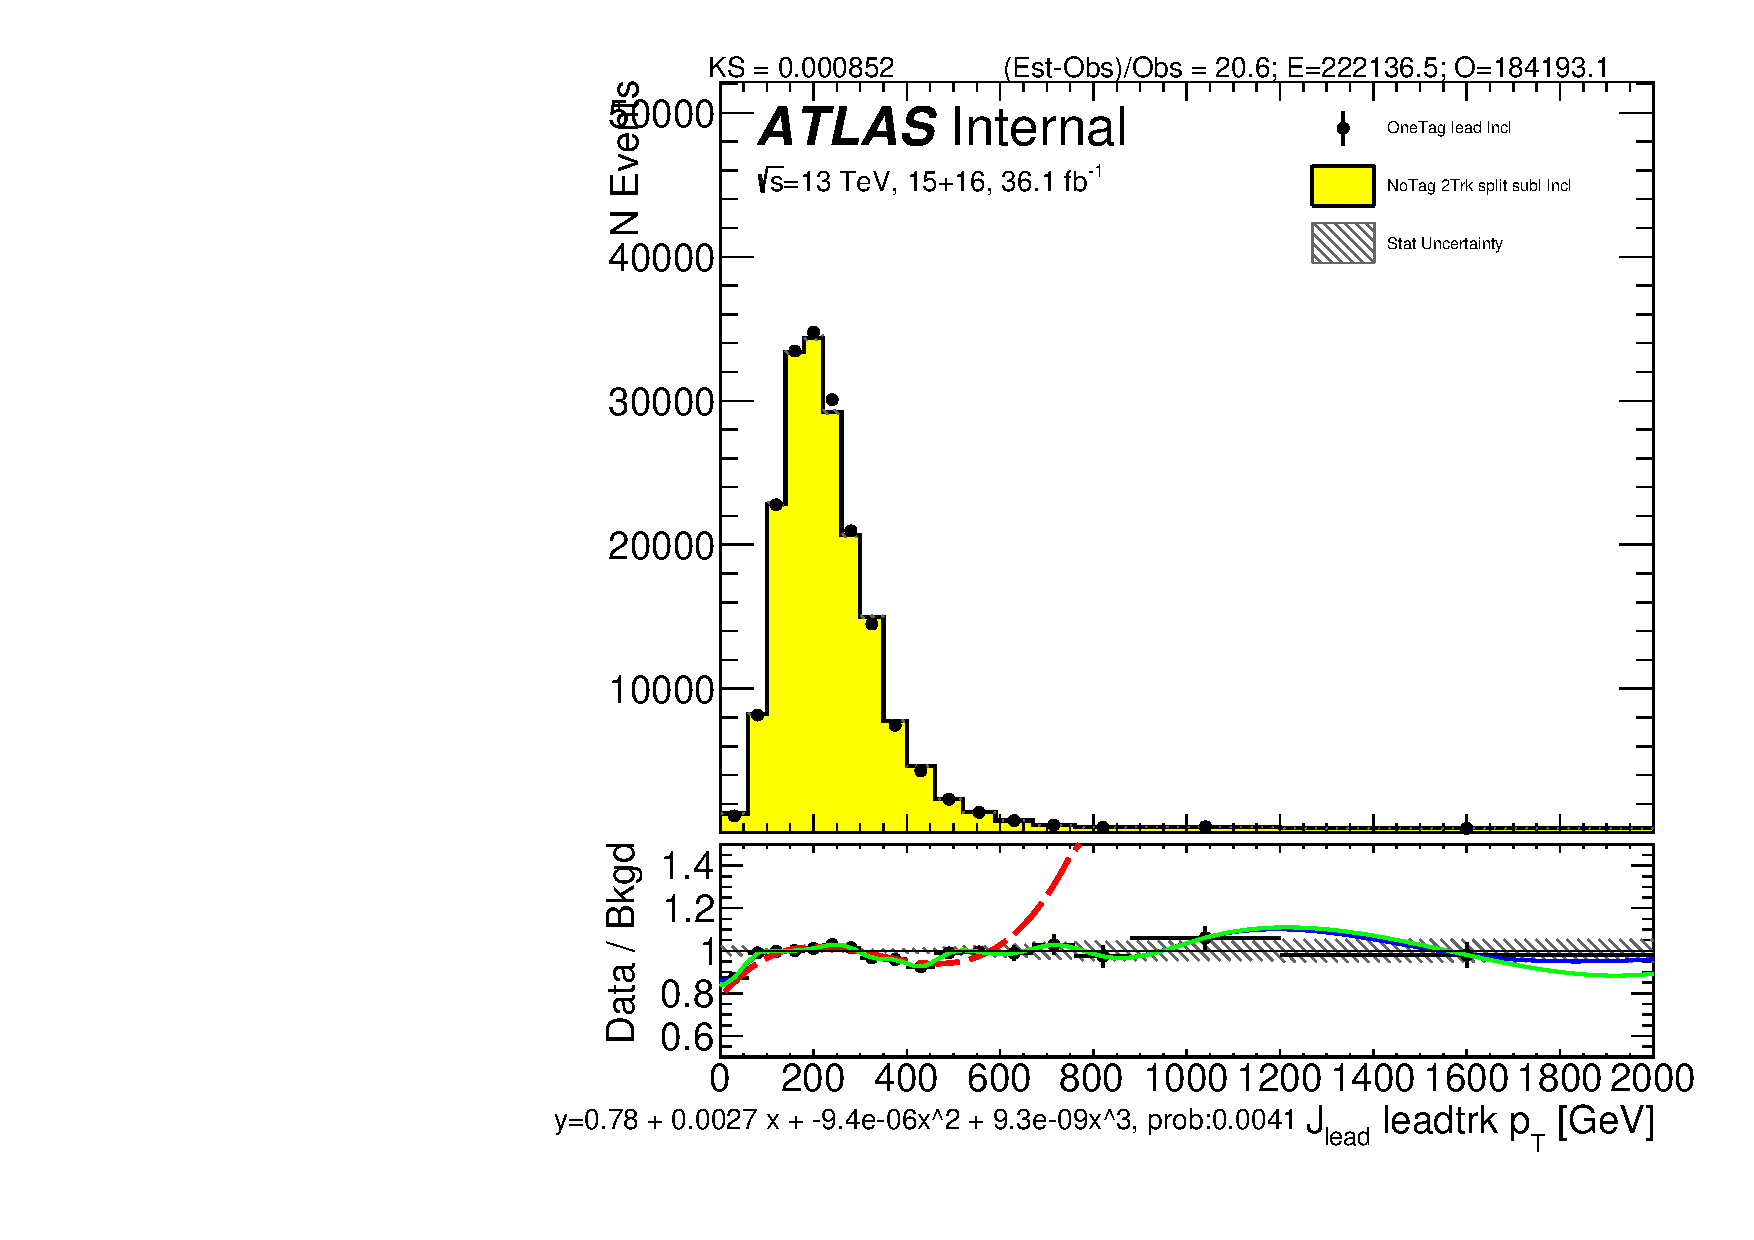
\includegraphics[width=0.32\textwidth,angle=-90]{figures/boosted/Reweight/Fits/Moriond_bkg_0_NoTag_2Trk_split_subl_Incl_leadHCand_trk0_Pt.pdf}
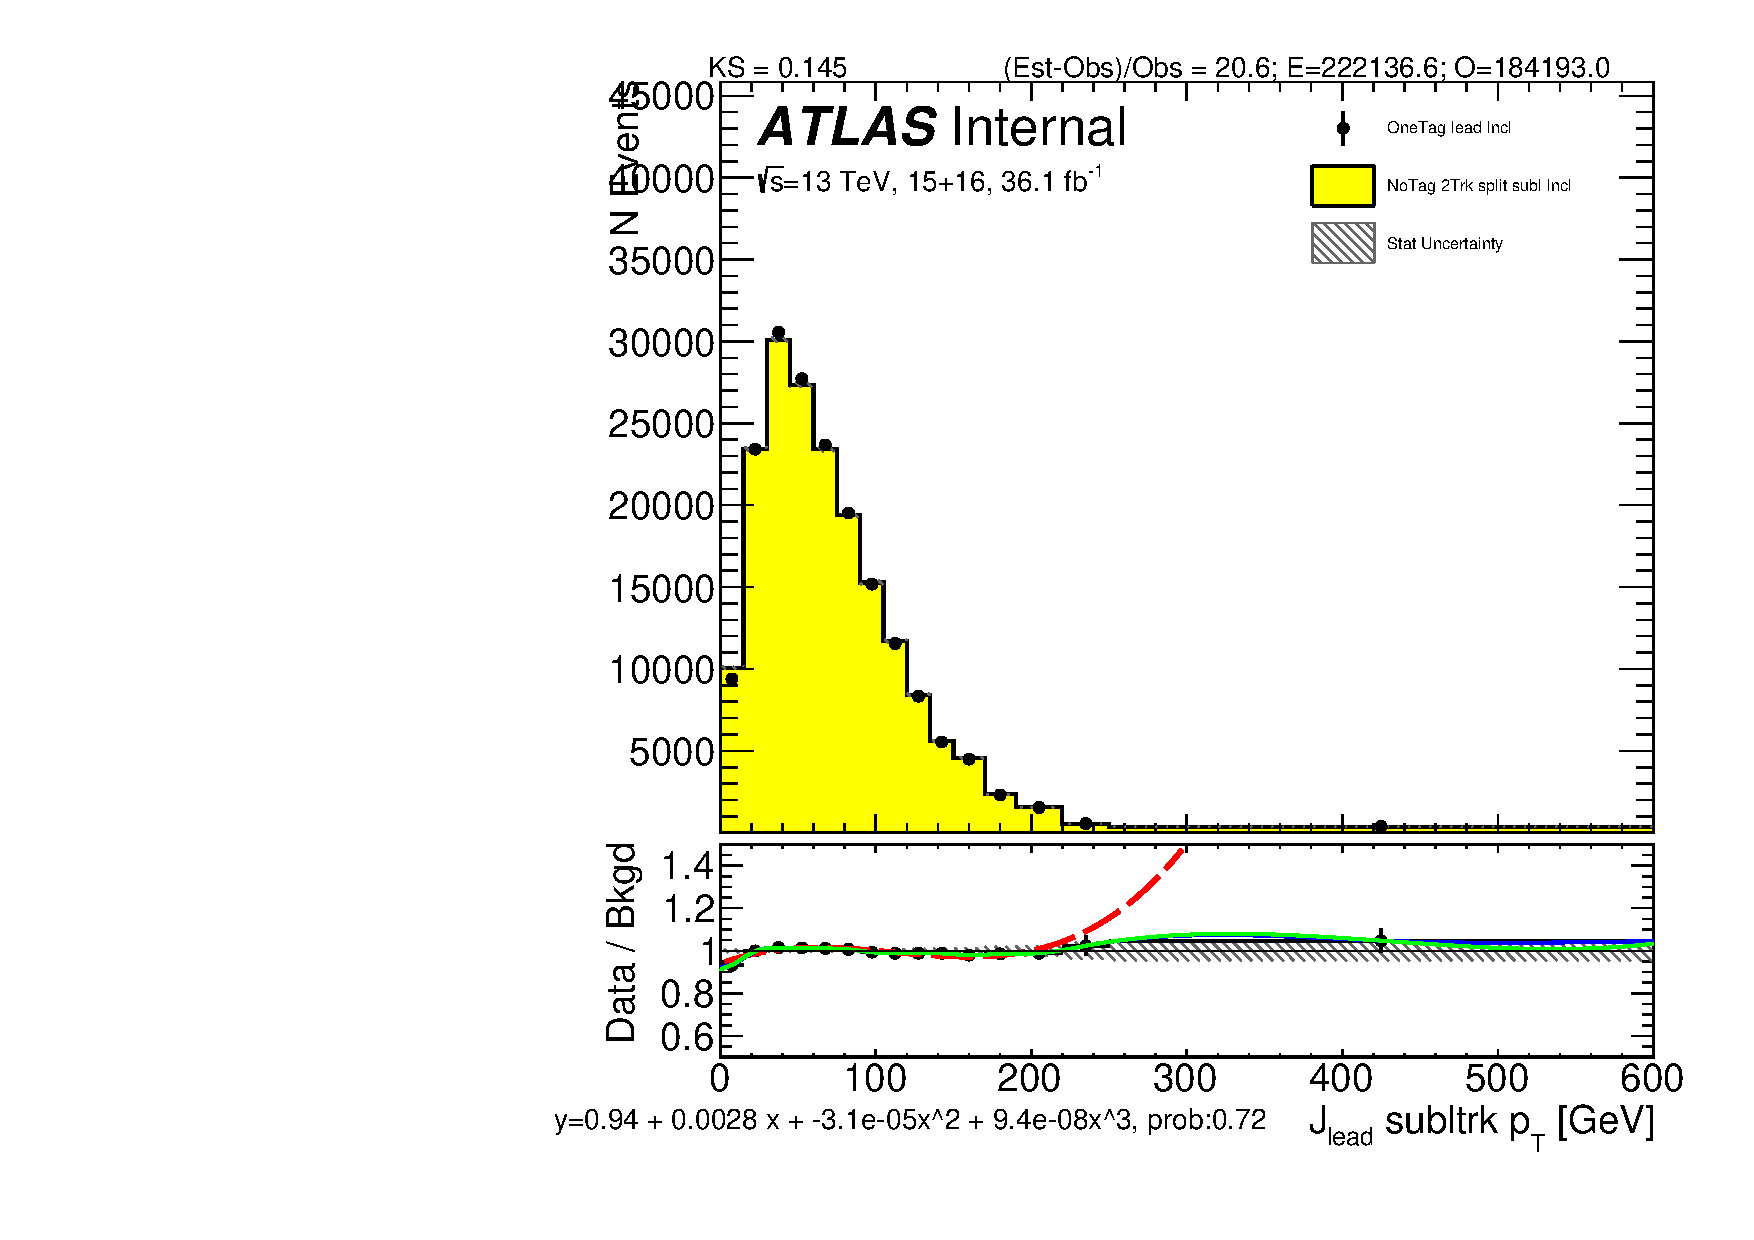
\includegraphics[width=0.32\textwidth,angle=-90]{figures/boosted/Reweight/Fits/Moriond_bkg_0_NoTag_2Trk_split_subl_Incl_leadHCand_trk1_Pt.pdf} \\
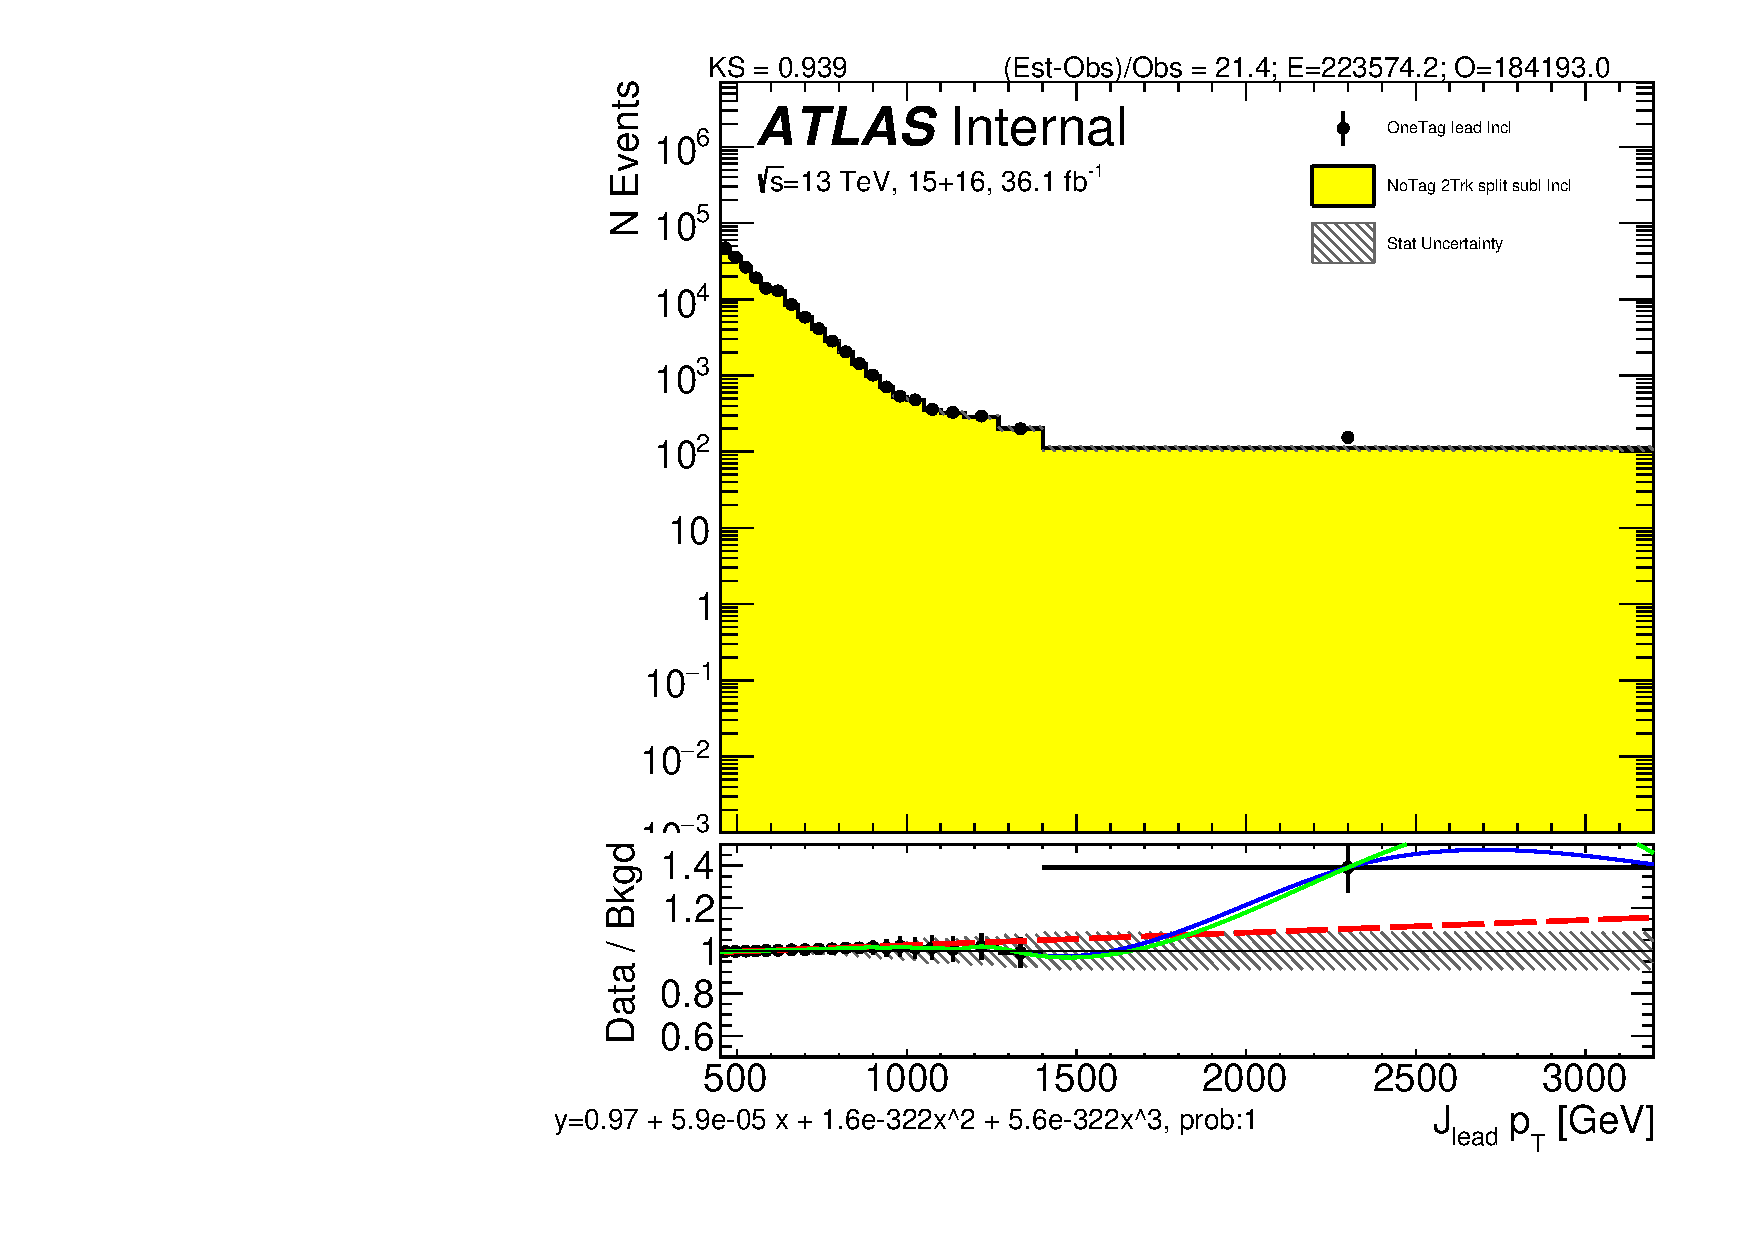
\includegraphics[width=0.32\textwidth,angle=-90]{figures/boosted/Reweight/Fits/Moriond_bkg_3_NoTag_2Trk_split_subl_Incl_leadHCand_Pt_m_1.pdf}
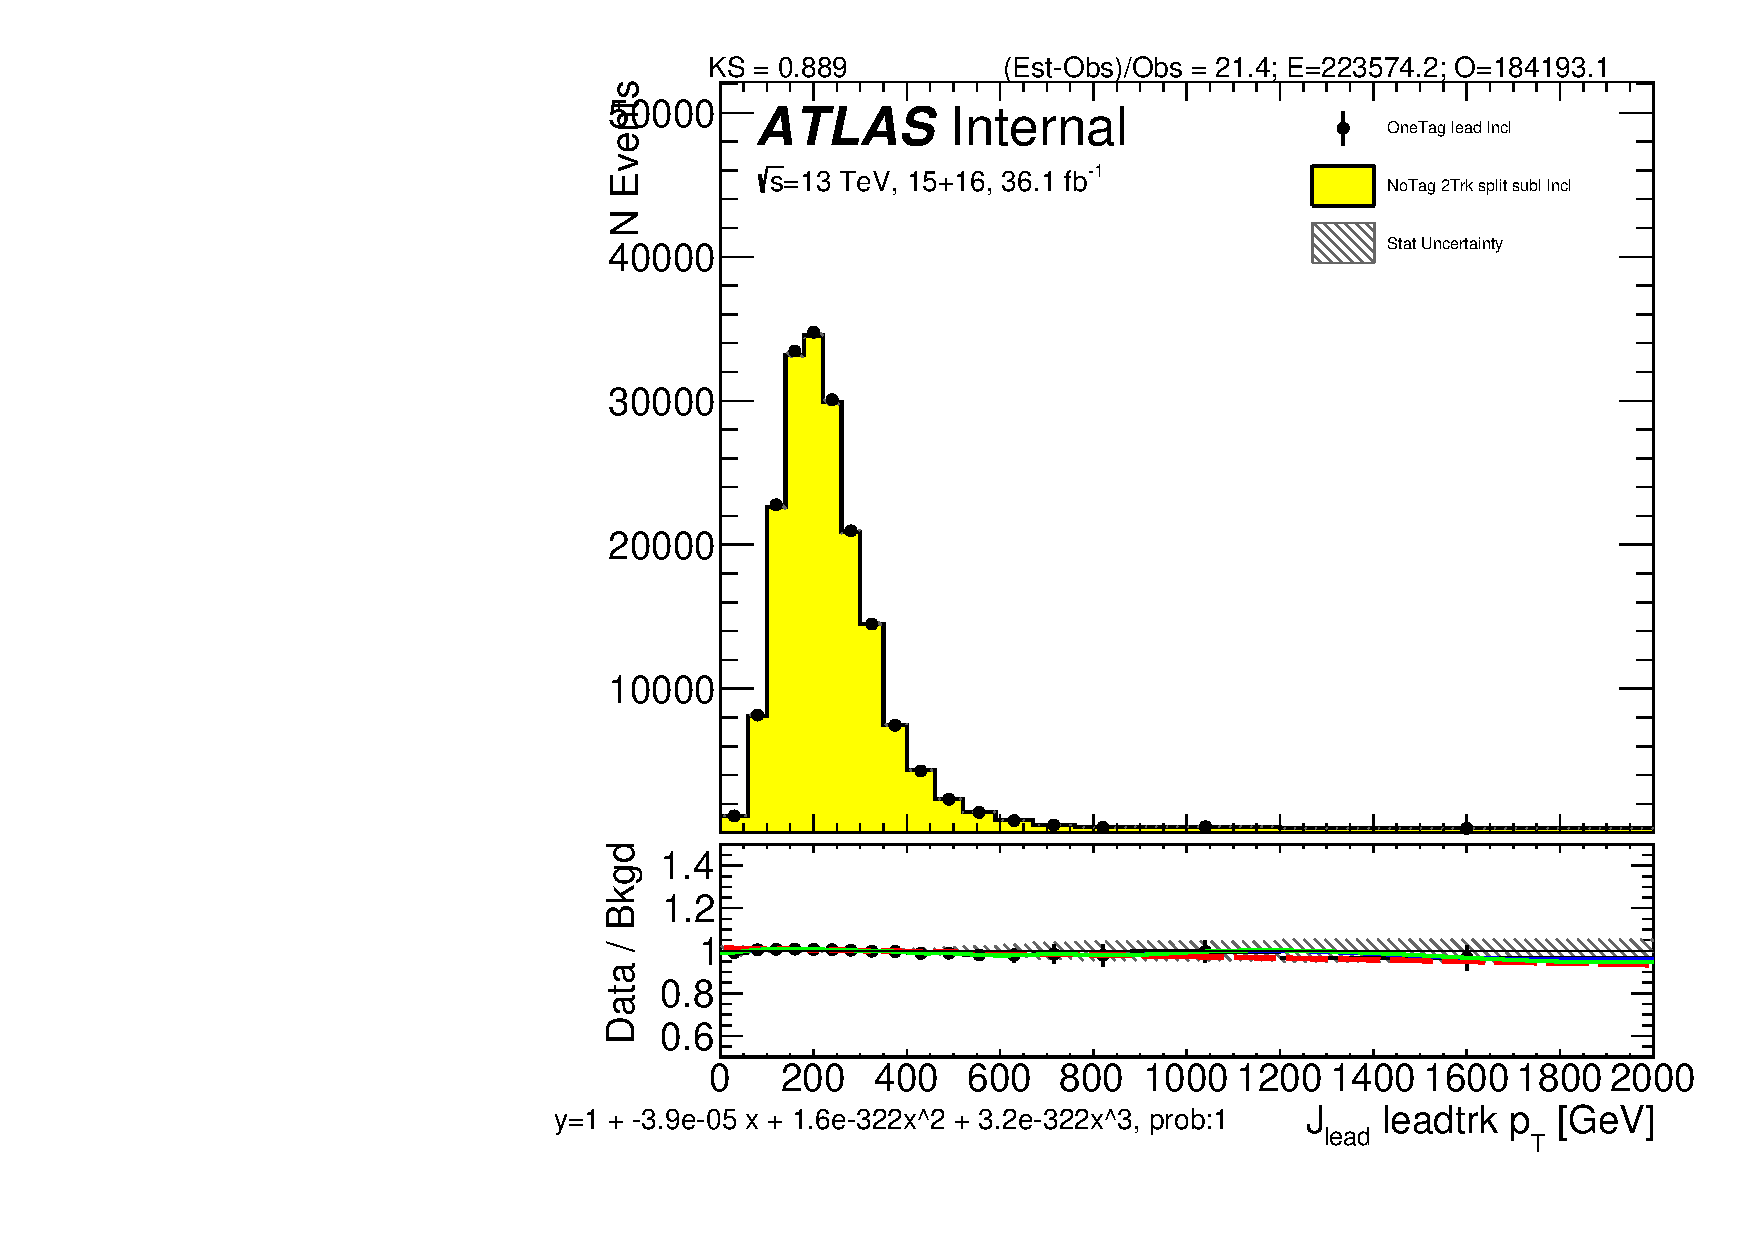
\includegraphics[width=0.32\textwidth,angle=-90]{figures/boosted/Reweight/Fits/Moriond_bkg_3_NoTag_2Trk_split_subl_Incl_leadHCand_trk0_Pt.pdf}
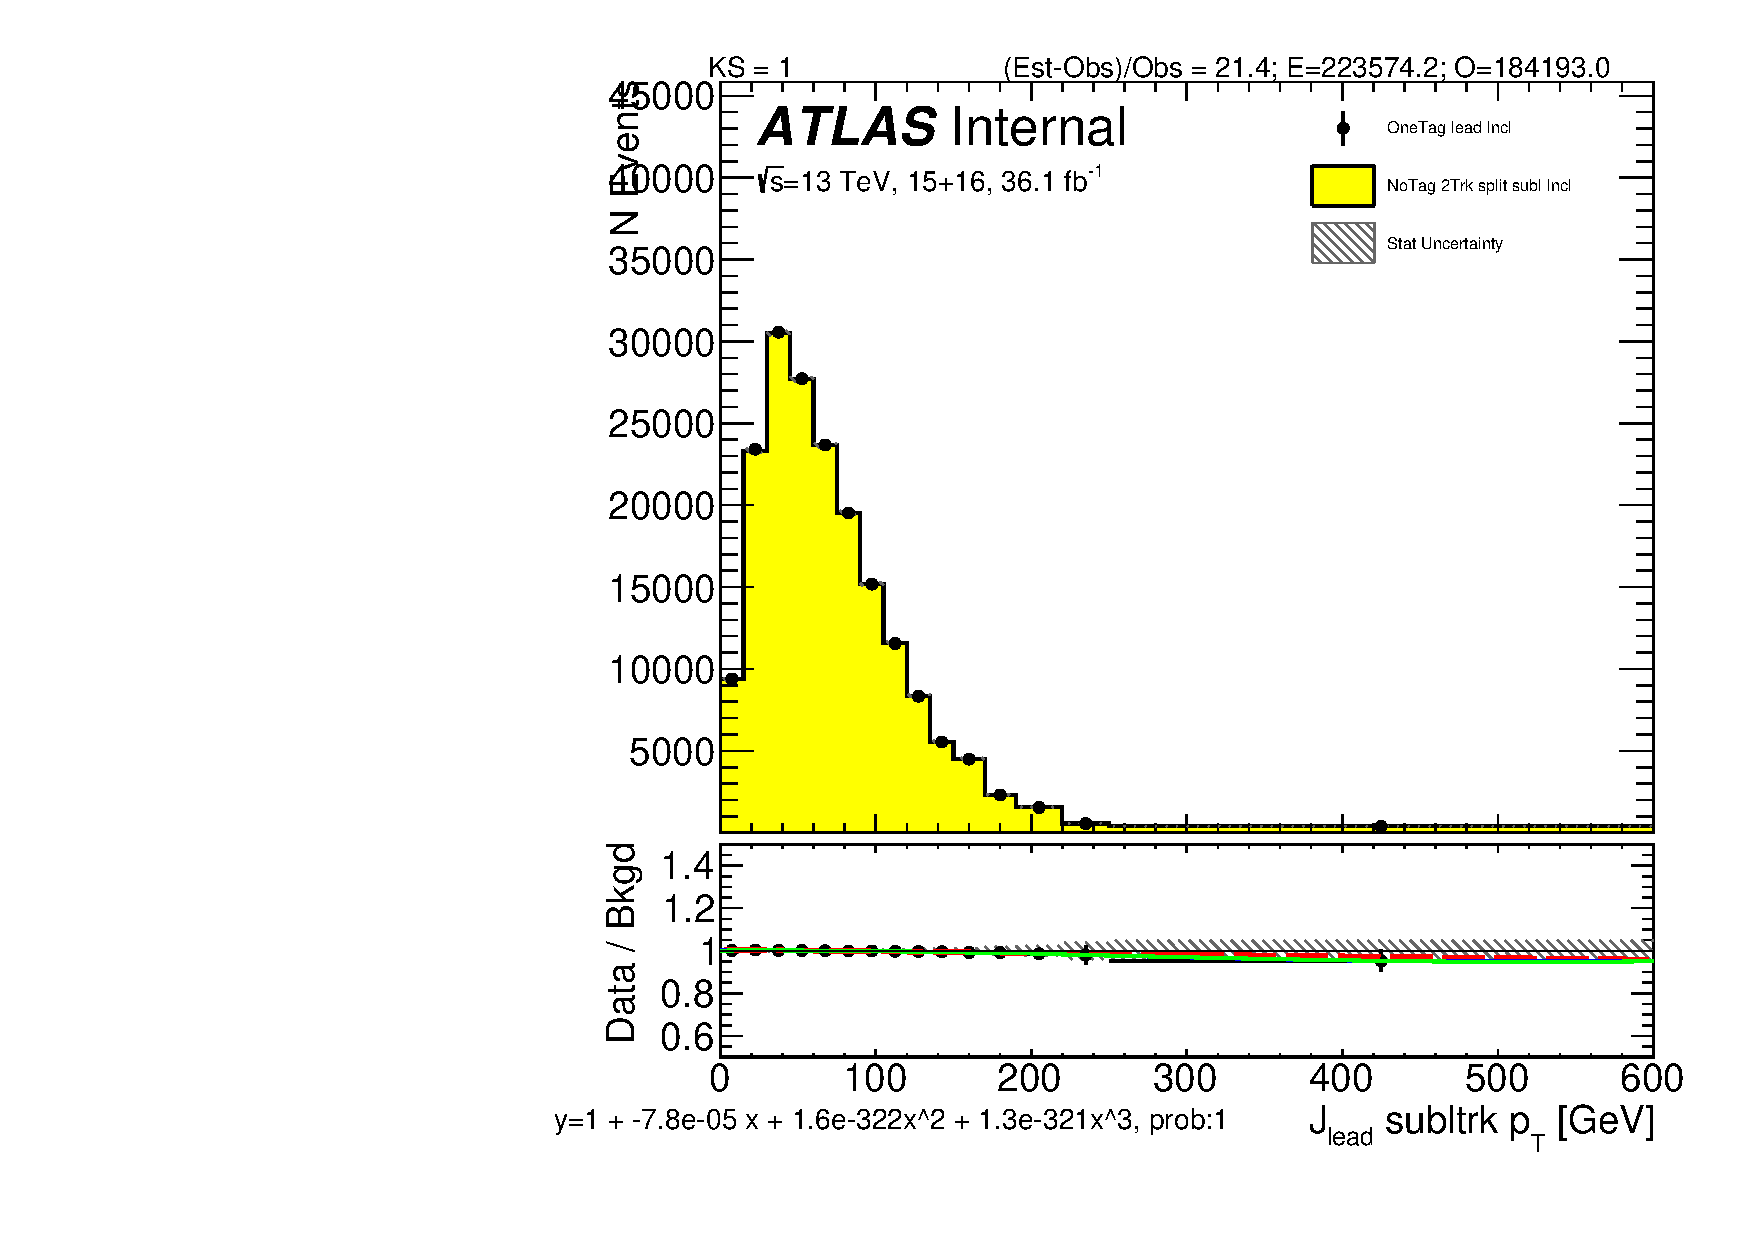
\includegraphics[width=0.32\textwidth,angle=-90]{figures/boosted/Reweight/Fits/Moriond_bkg_3_NoTag_2Trk_split_subl_Incl_leadHCand_trk1_Pt.pdf} \\
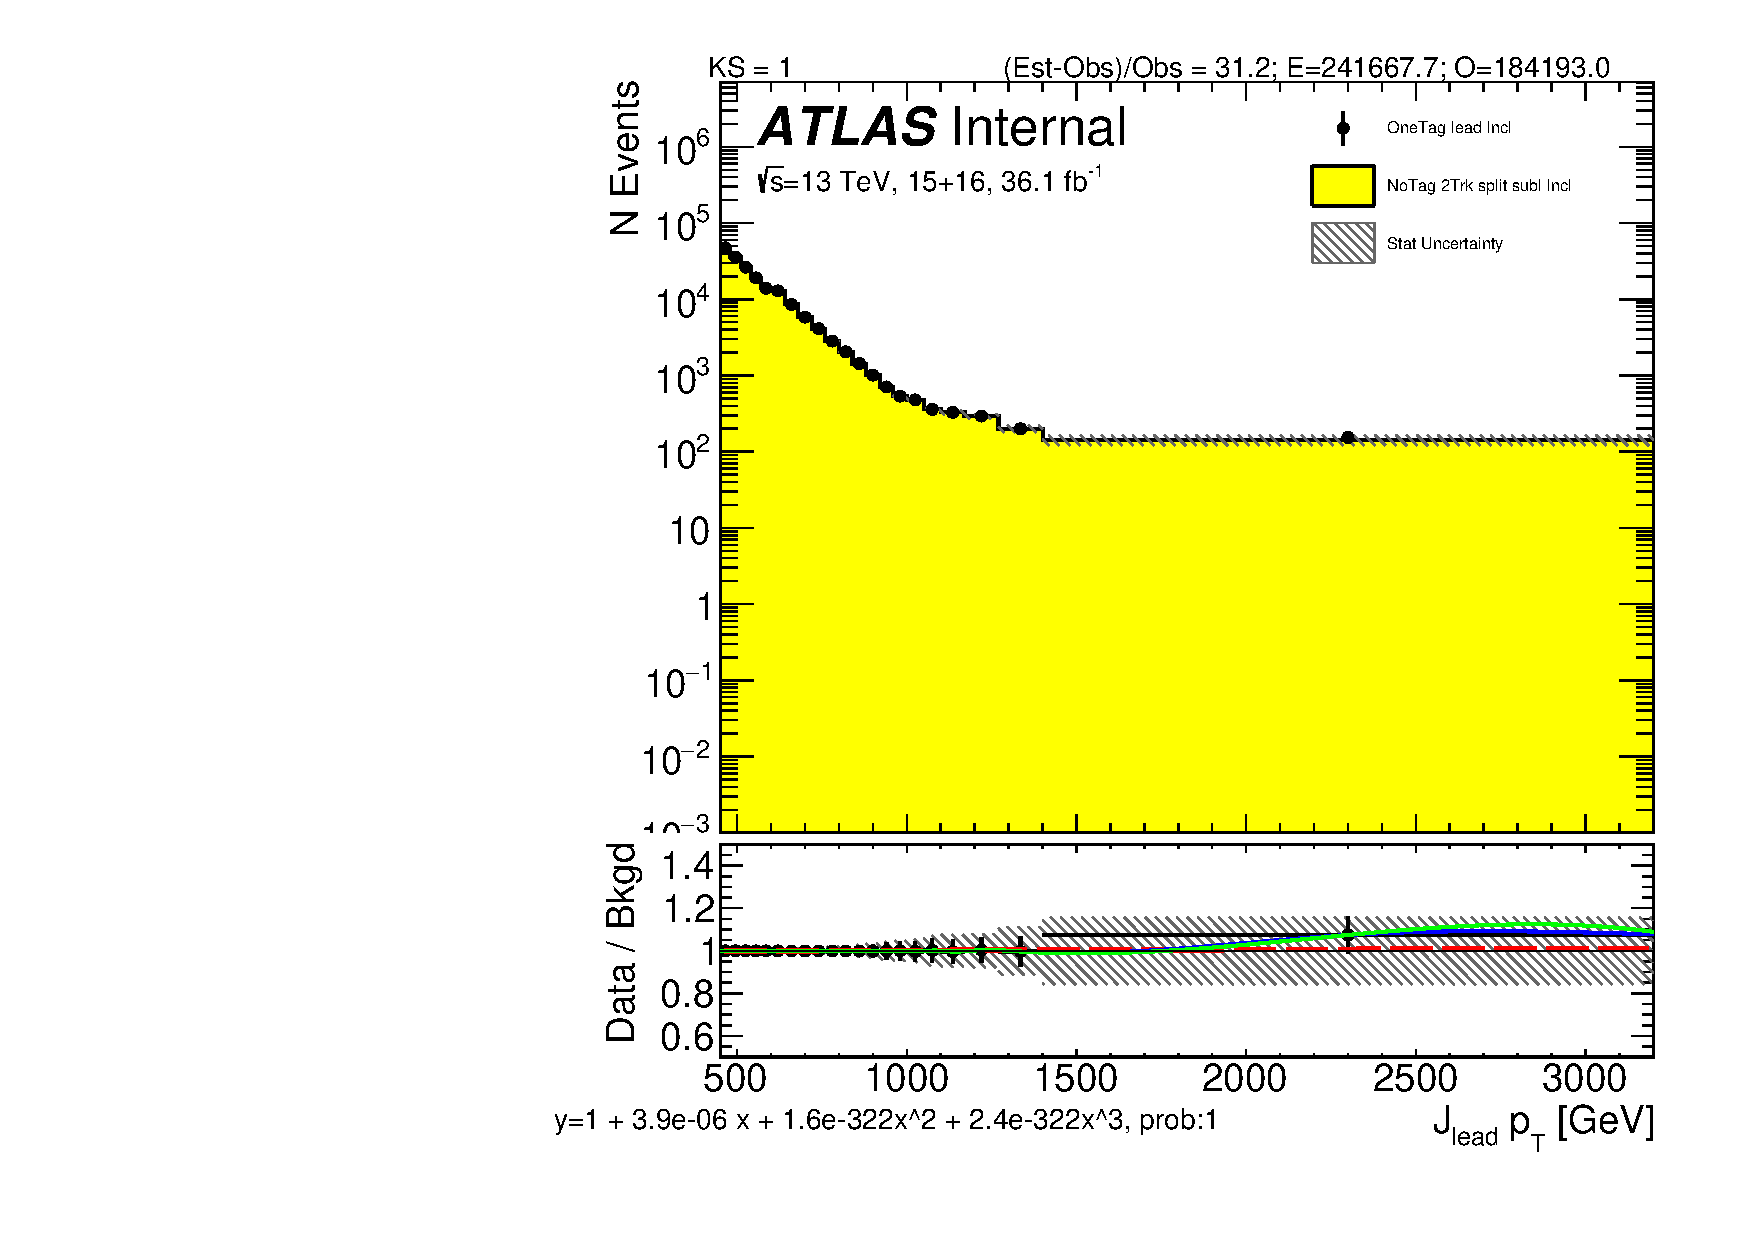
\includegraphics[width=0.32\textwidth,angle=-90]{figures/boosted/Reweight/Fits/Moriond_bkg_9_NoTag_2Trk_split_subl_Incl_leadHCand_Pt_m_1.pdf}
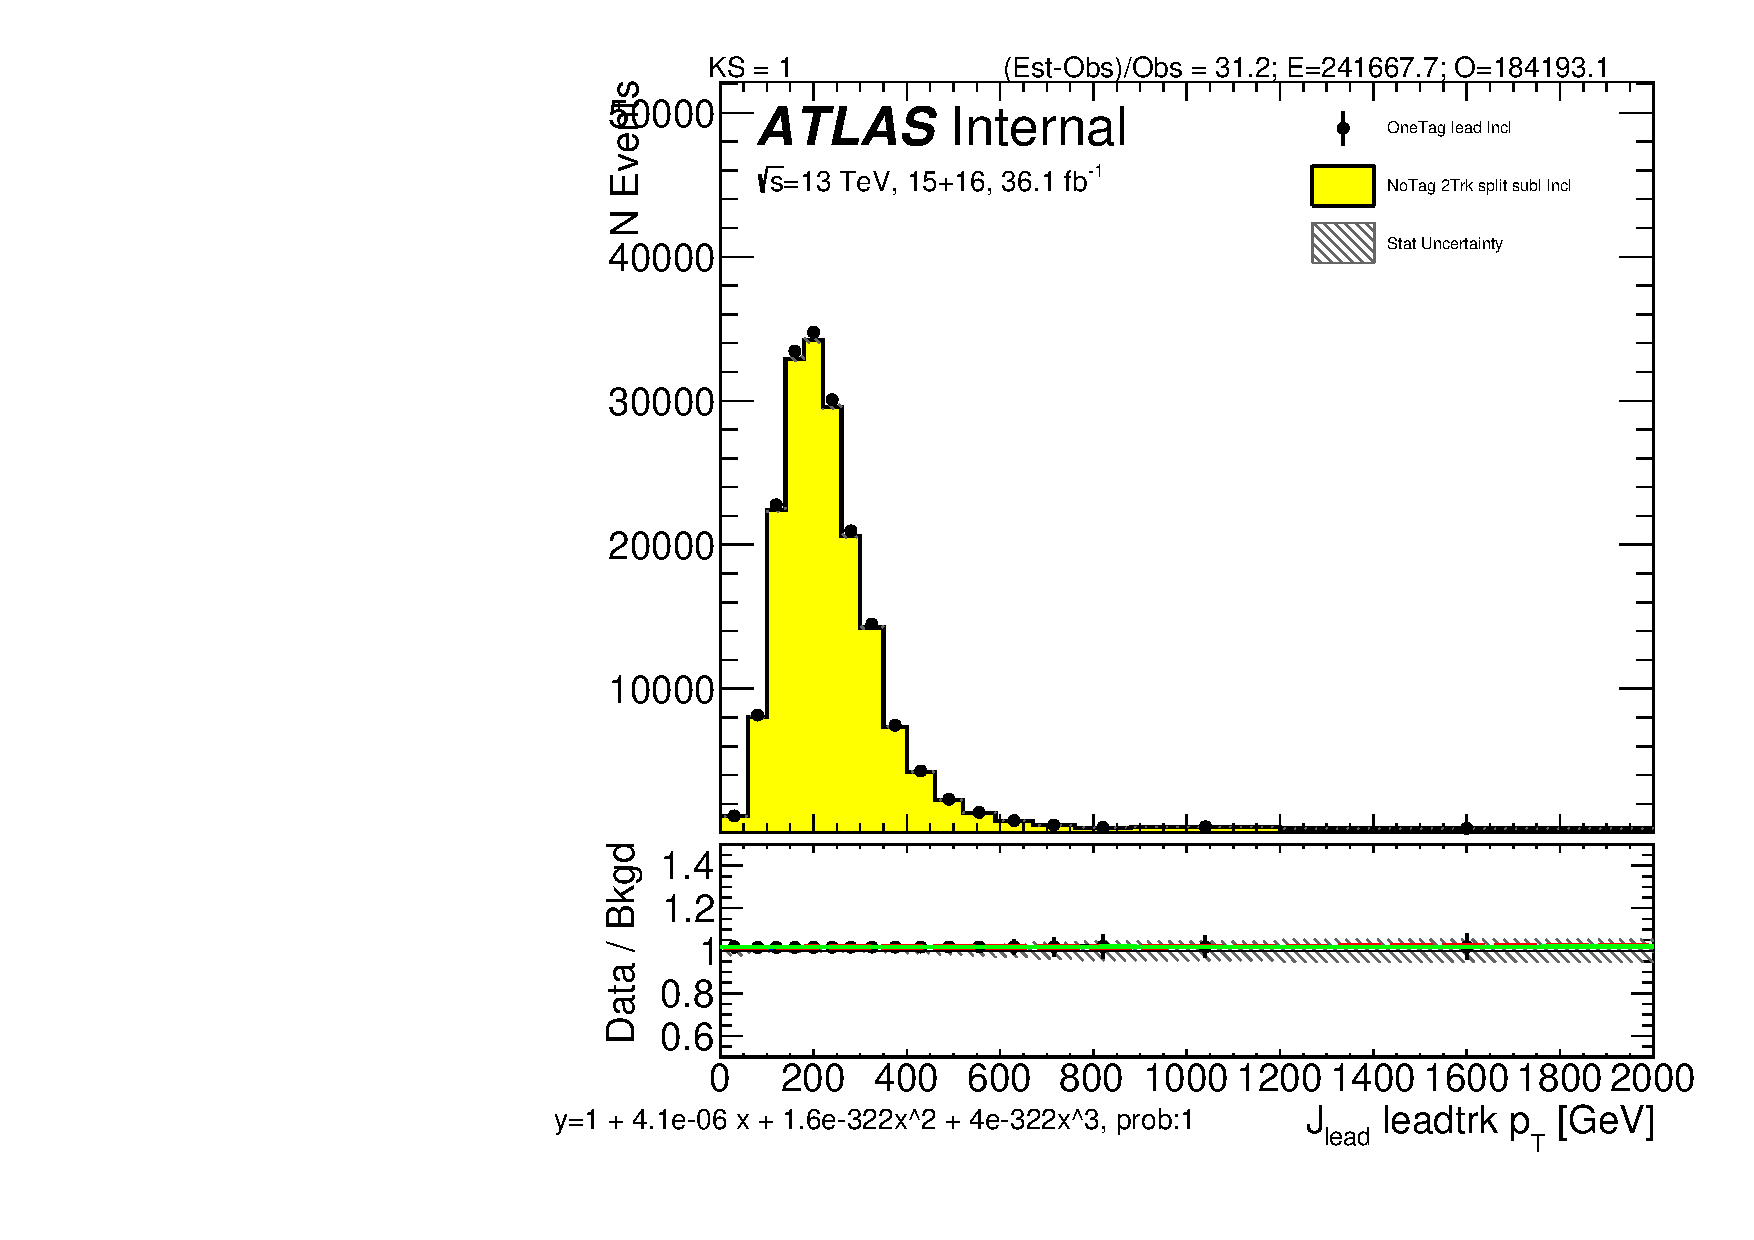
\includegraphics[width=0.32\textwidth,angle=-90]{figures/boosted/Reweight/Fits/Moriond_bkg_9_NoTag_2Trk_split_subl_Incl_leadHCand_trk0_Pt.pdf}
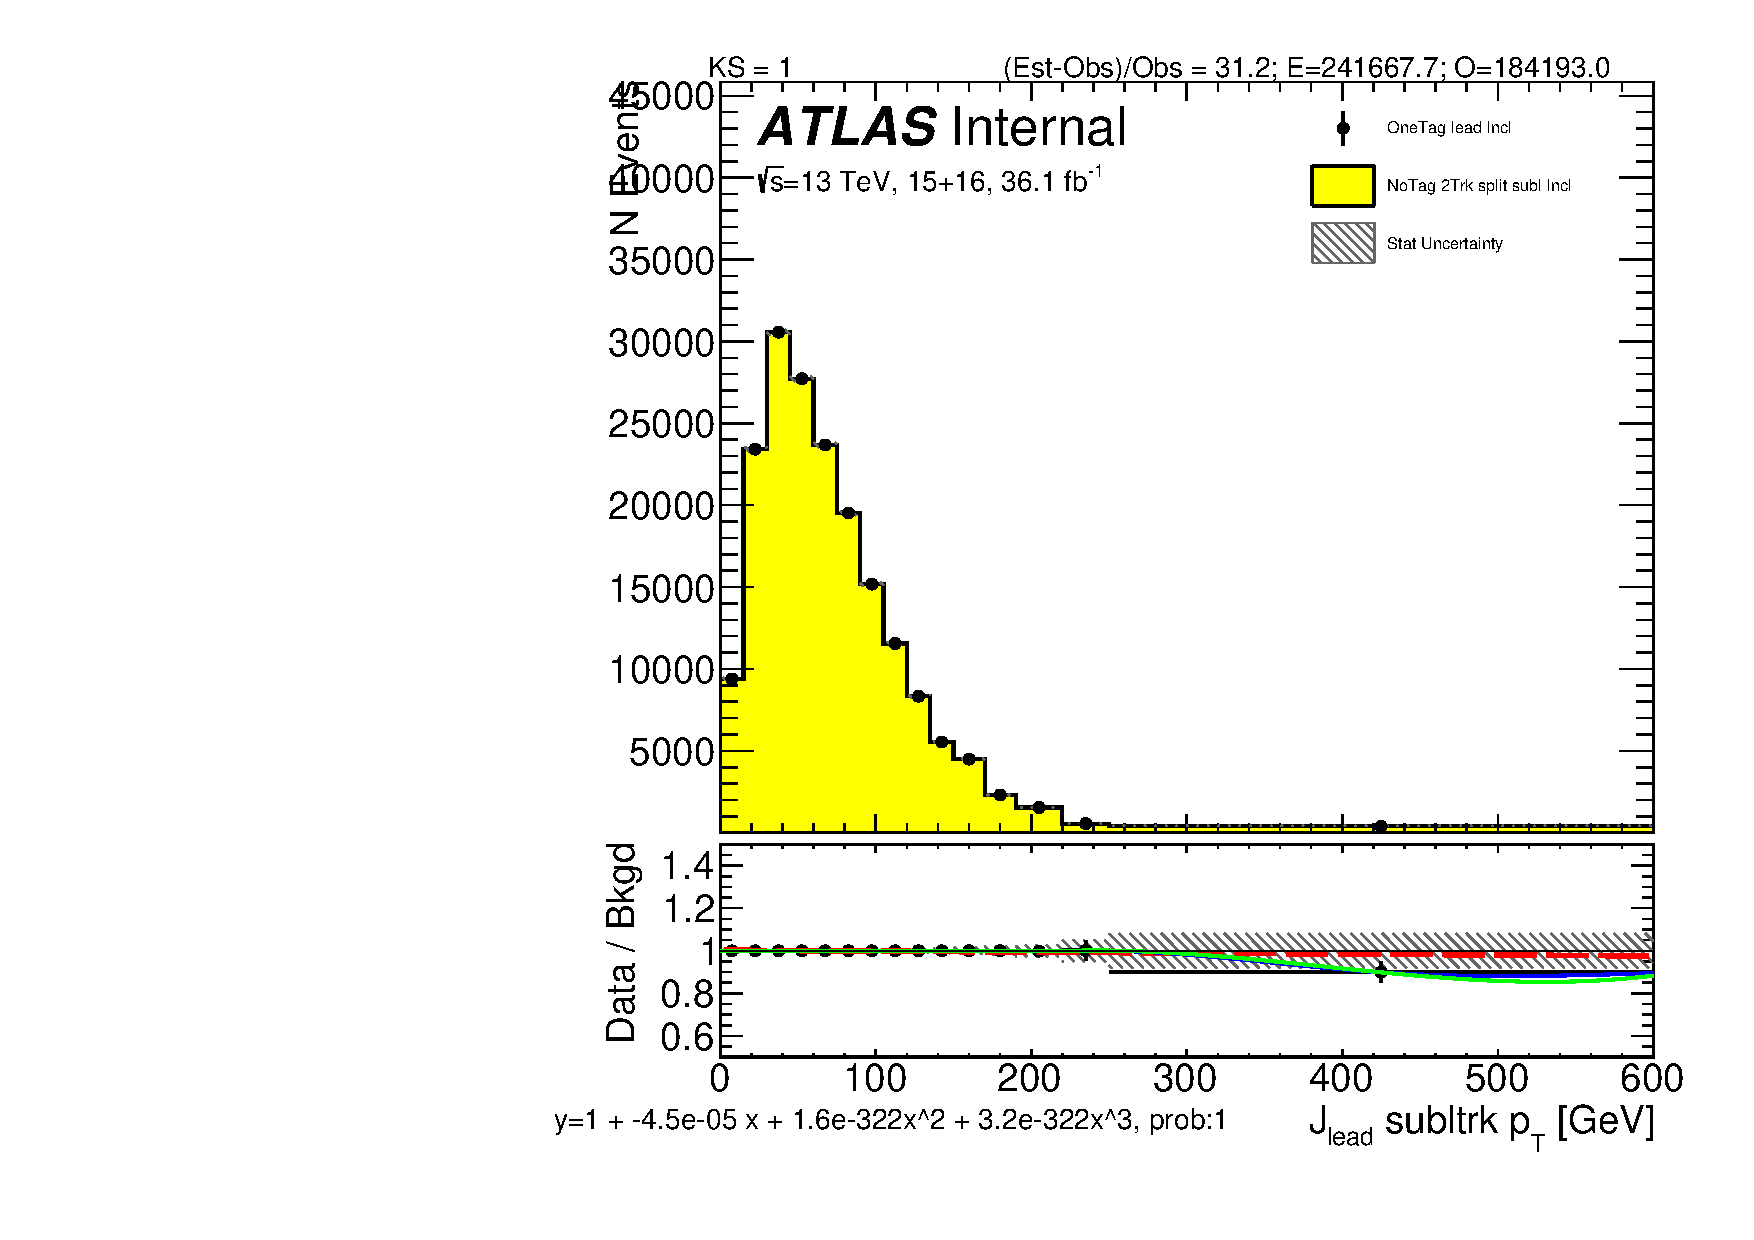
\includegraphics[width=0.32\textwidth,angle=-90]{figures/boosted/Reweight/Fits/Moriond_bkg_9_NoTag_2Trk_split_subl_Incl_leadHCand_trk1_Pt.pdf} \\
\caption{For $2b$s background estimate: the fits to the ratio of the data in the 1$b$ category, of the leading Higgs candidate 1$b$-tagged events's leading Higgs candidate distributions(black point), over the sublleading Higgs candidate 1$b$-tagged events's leading Higgs candidate distributions(yellow). Distributions and fits to the estimated QCD background for large-$R$ jet $p_{T}$ (left),  the large-$R$ jet's leading trackjet $p_T$ (middle), and large-$R$ jet's subleading trackjet $p_T$ (right) are shown.  Figure are shown before reweighting (top row), after the first iteration(second row), after the fourth iteration(third row), and after the last iteration (bottow row). The green line is the spline extrapolation; and the red line is a polynomial fit.}
\label{fig:rw-2bs-subl}
\end{center}
\end{figure*}

\begin{figure*}[htbp!]
\begin{center}
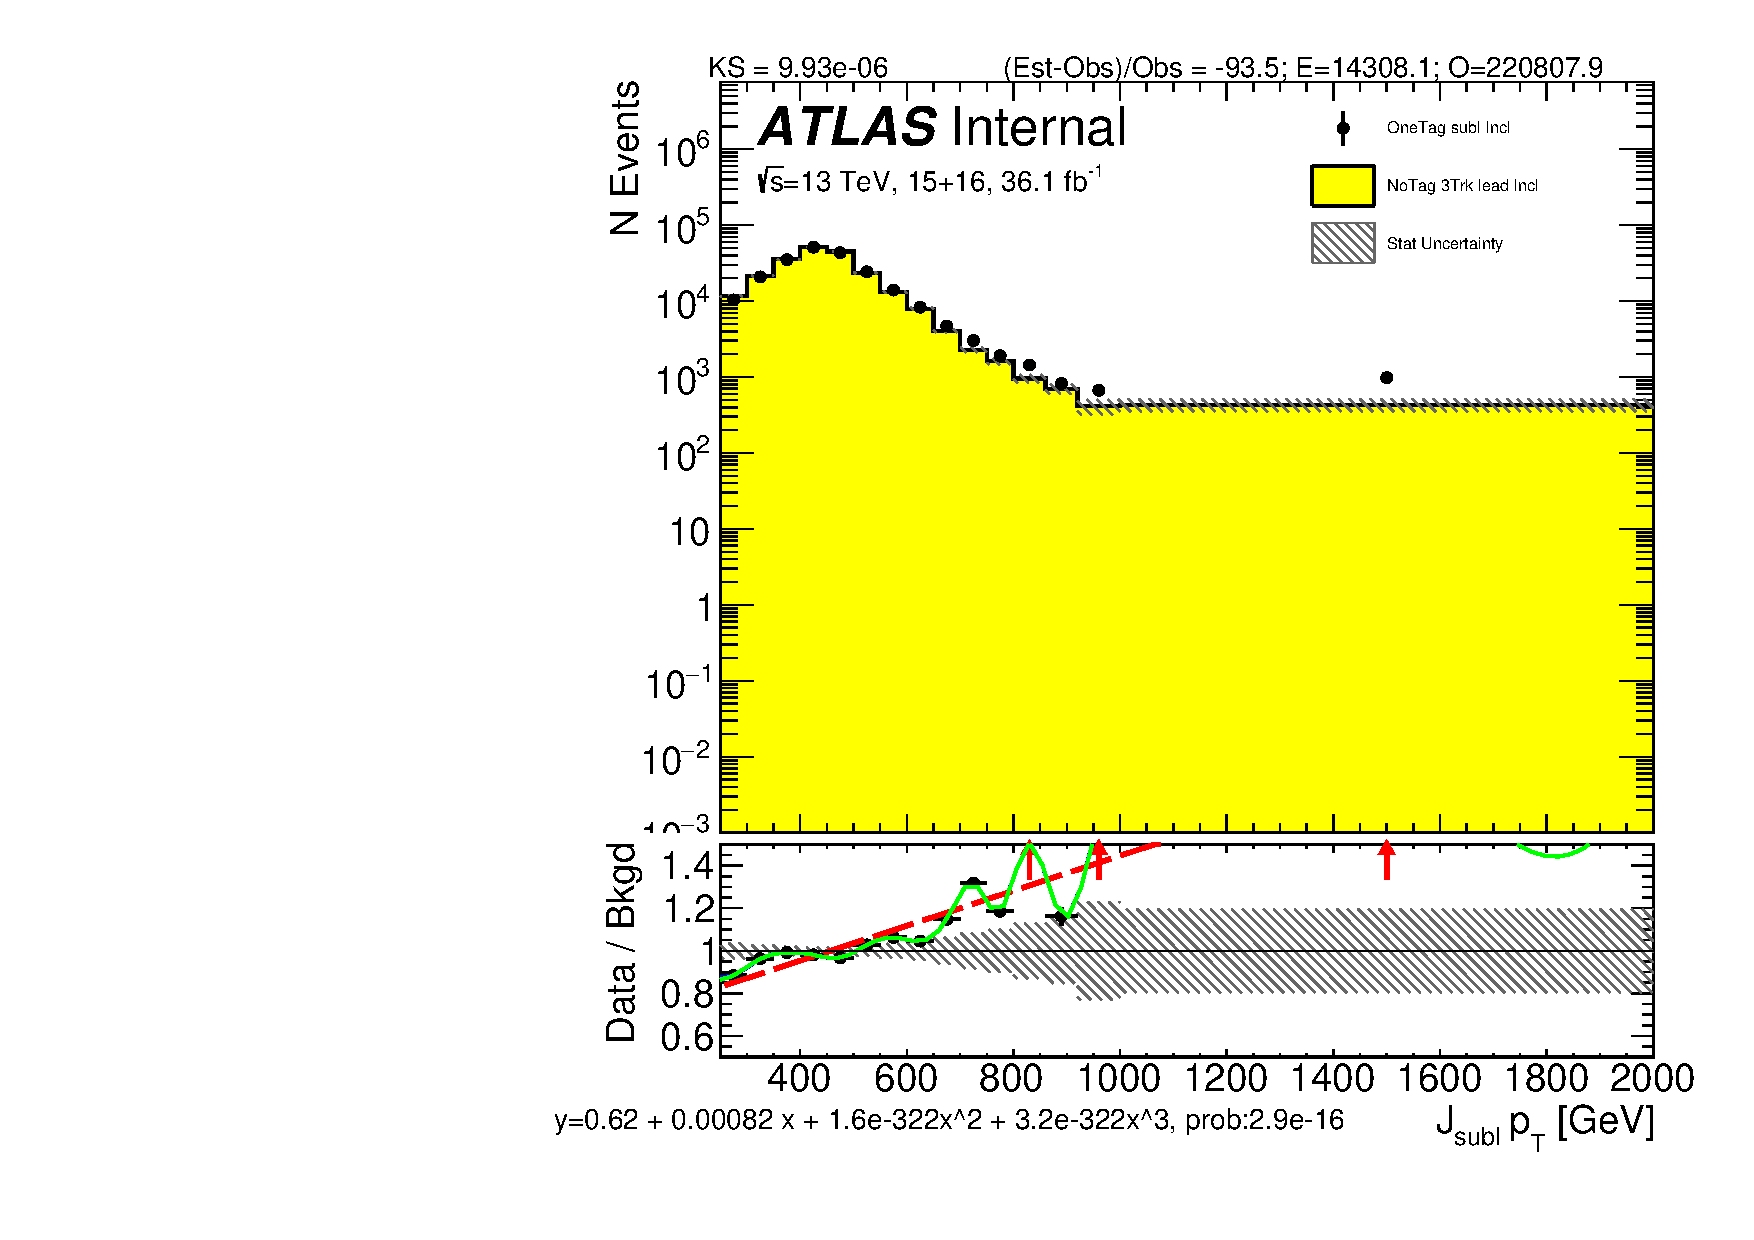
\includegraphics[width=0.32\textwidth,angle=-90]{figures/boosted/Reweight/Fits/Moriond_NoTag_3Trk_lead_Incl_sublHCand_Pt_m_1.pdf}
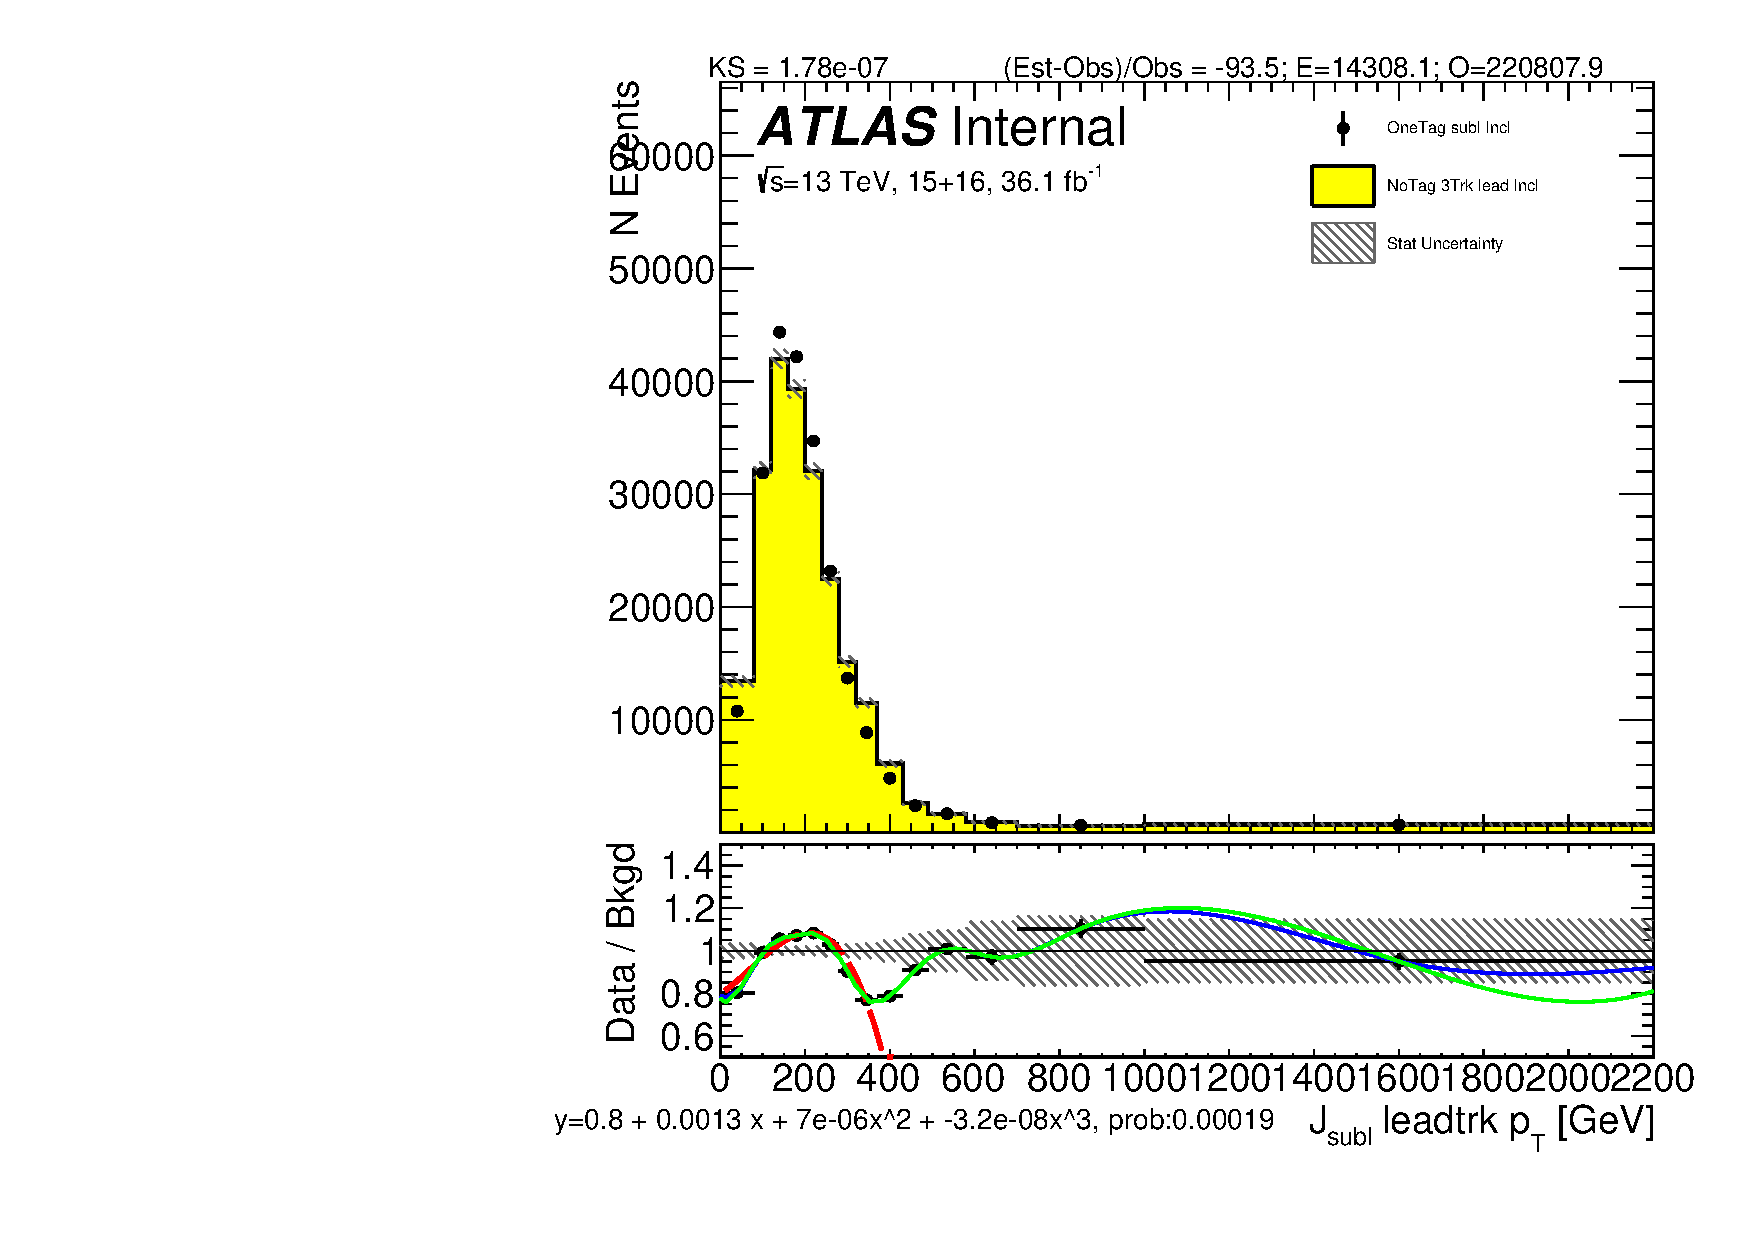
\includegraphics[width=0.32\textwidth,angle=-90]{figures/boosted/Reweight/Fits/Moriond_NoTag_3Trk_lead_Incl_sublHCand_trk0_Pt.pdf}
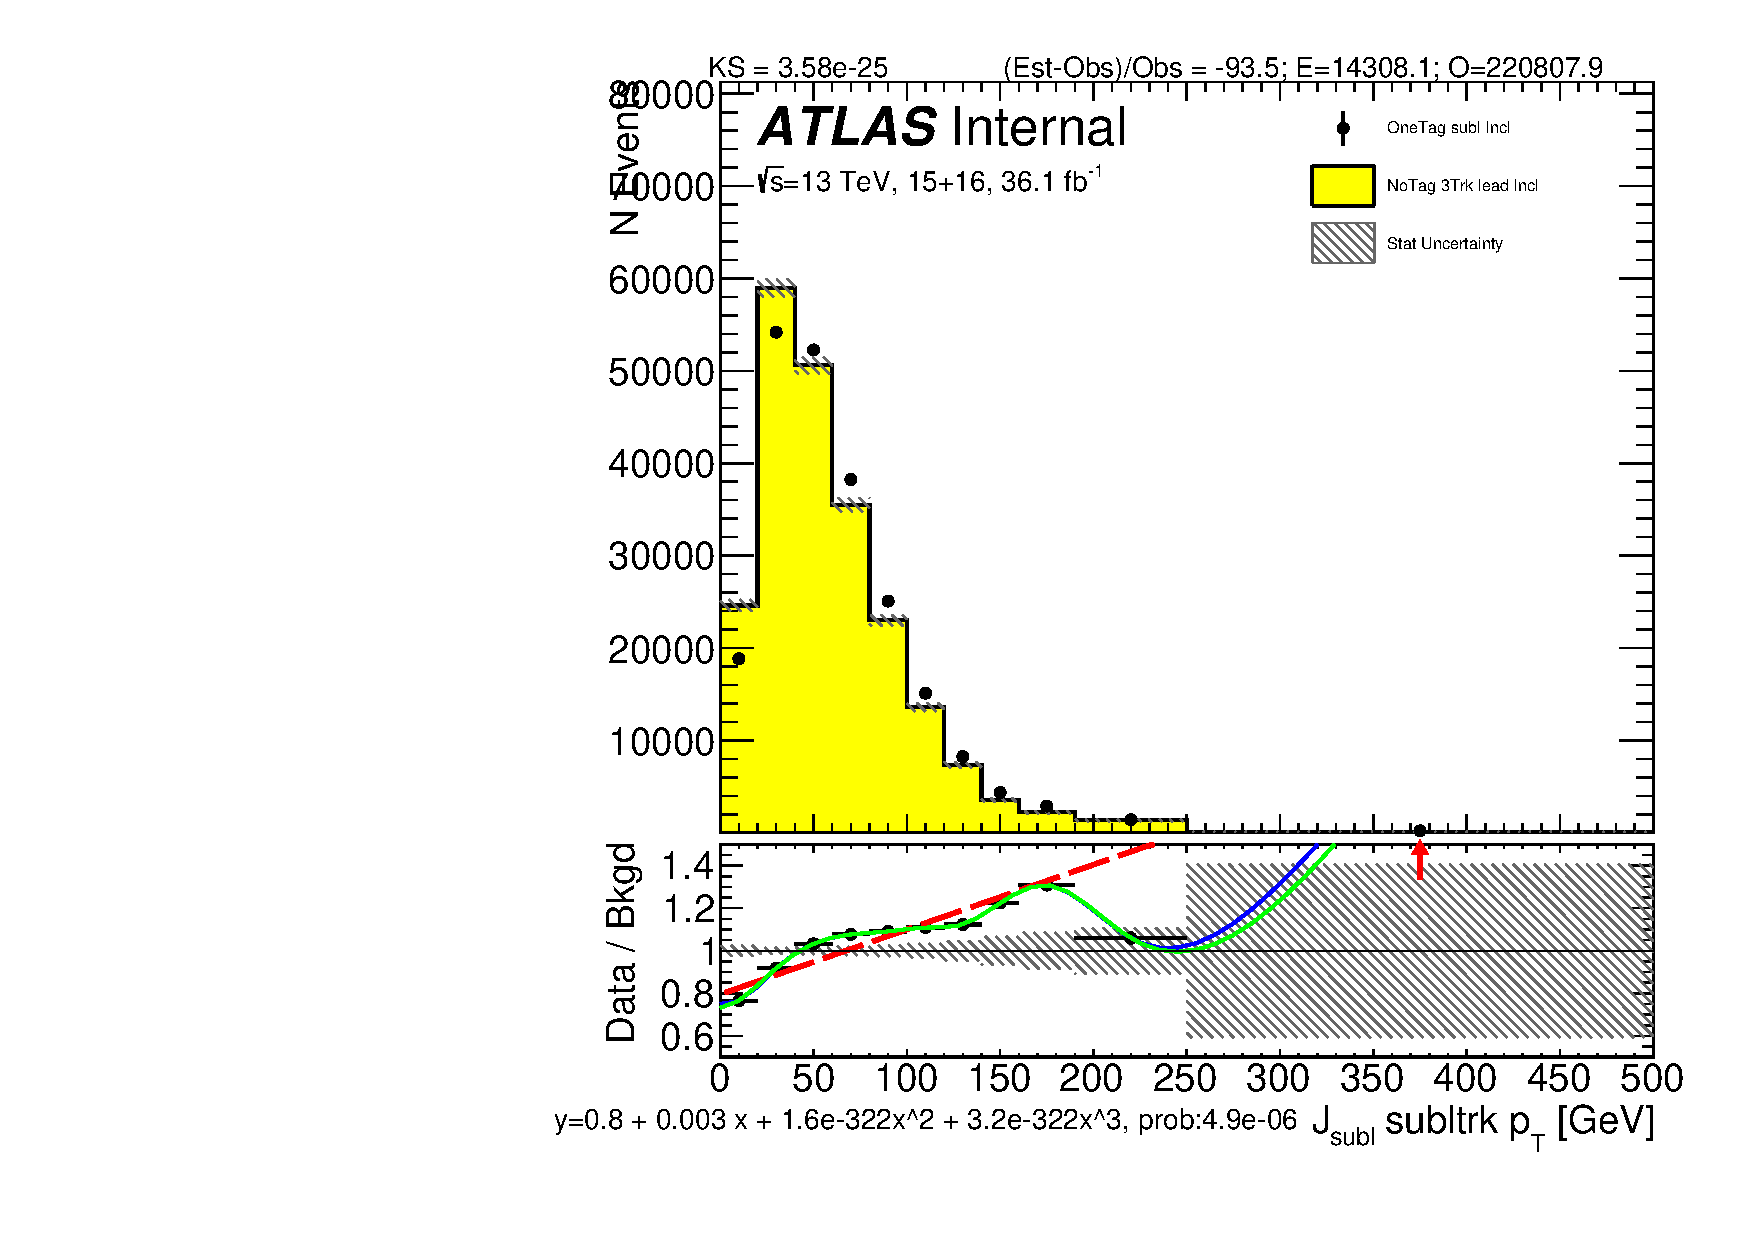
\includegraphics[width=0.32\textwidth,angle=-90]{figures/boosted/Reweight/Fits/Moriond_NoTag_3Trk_lead_Incl_sublHCand_trk1_Pt.pdf} \\
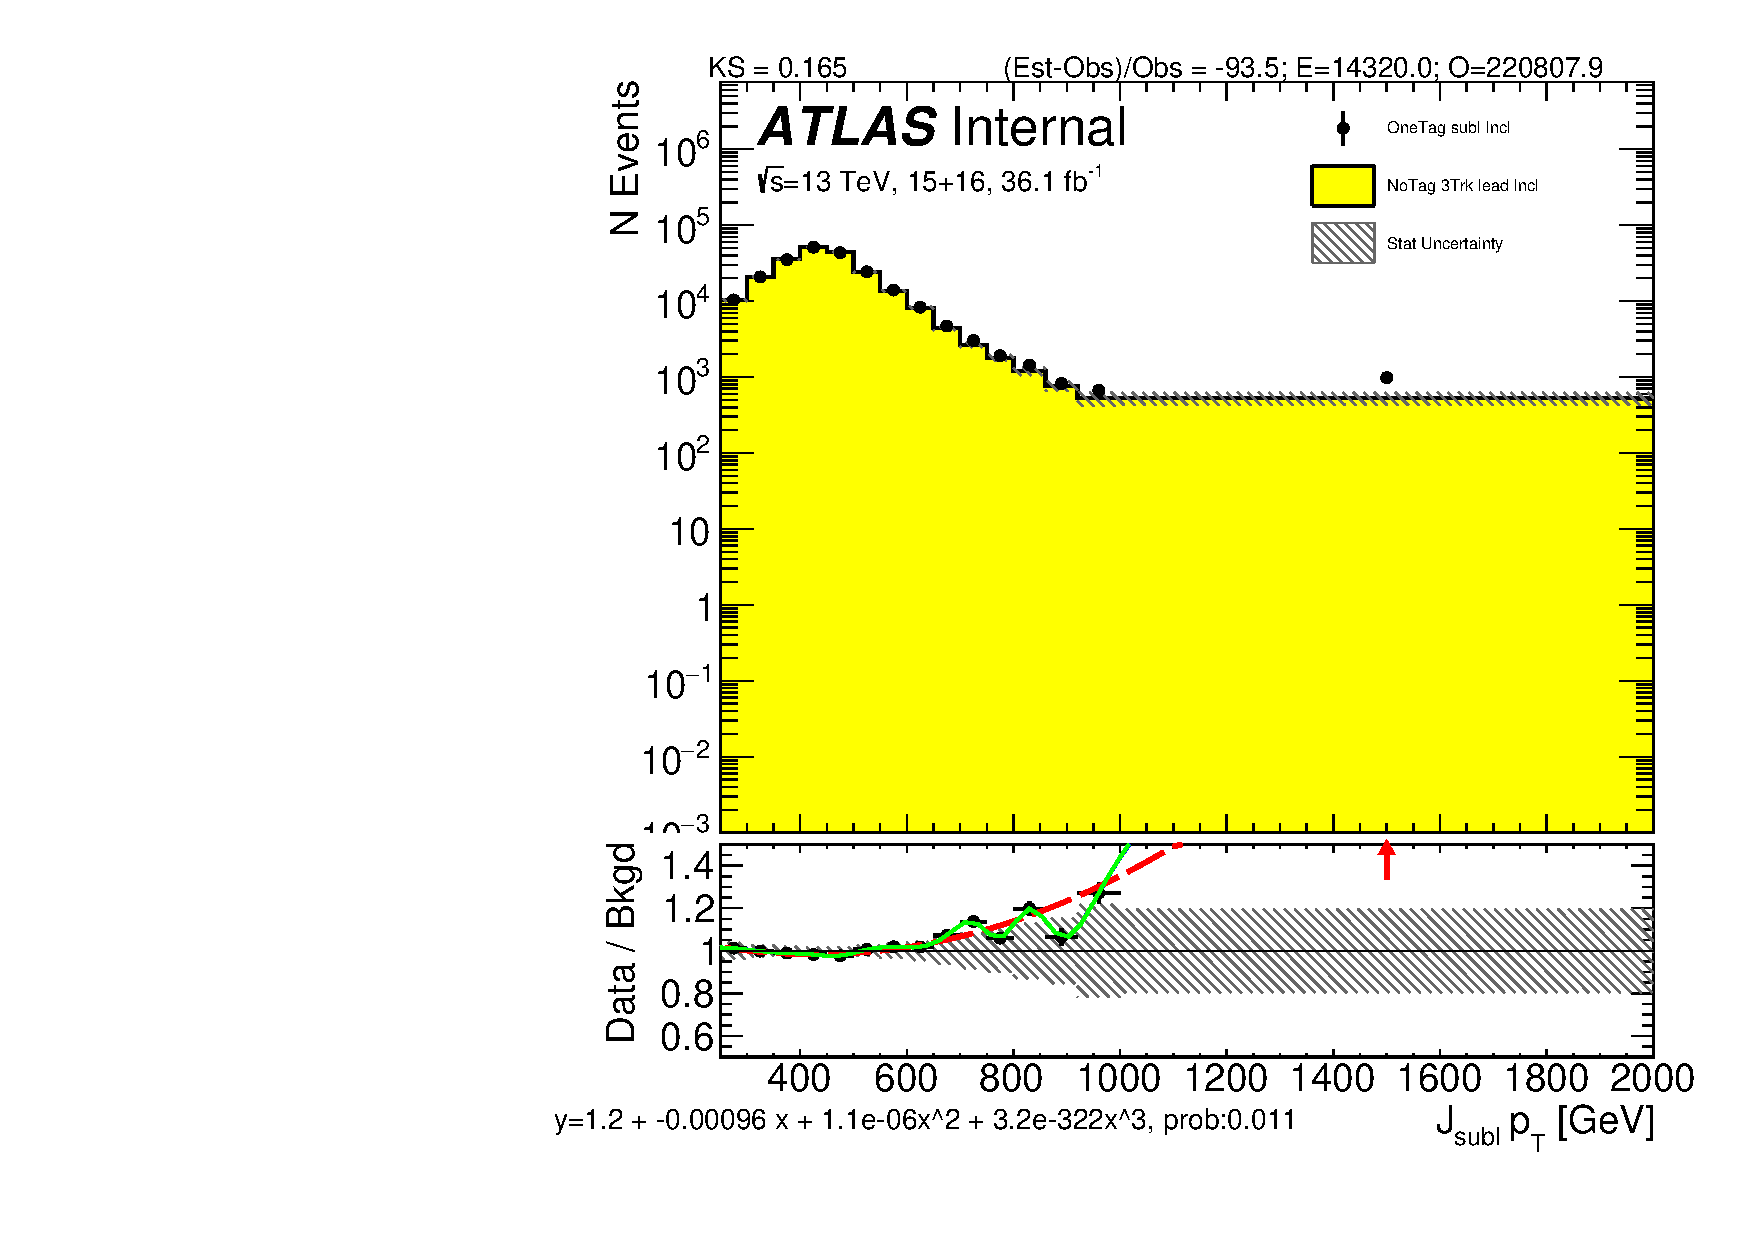
\includegraphics[width=0.32\textwidth,angle=-90]{figures/boosted/Reweight/Fits/Moriond_bkg_0_NoTag_3Trk_lead_Incl_sublHCand_Pt_m_1.pdf}
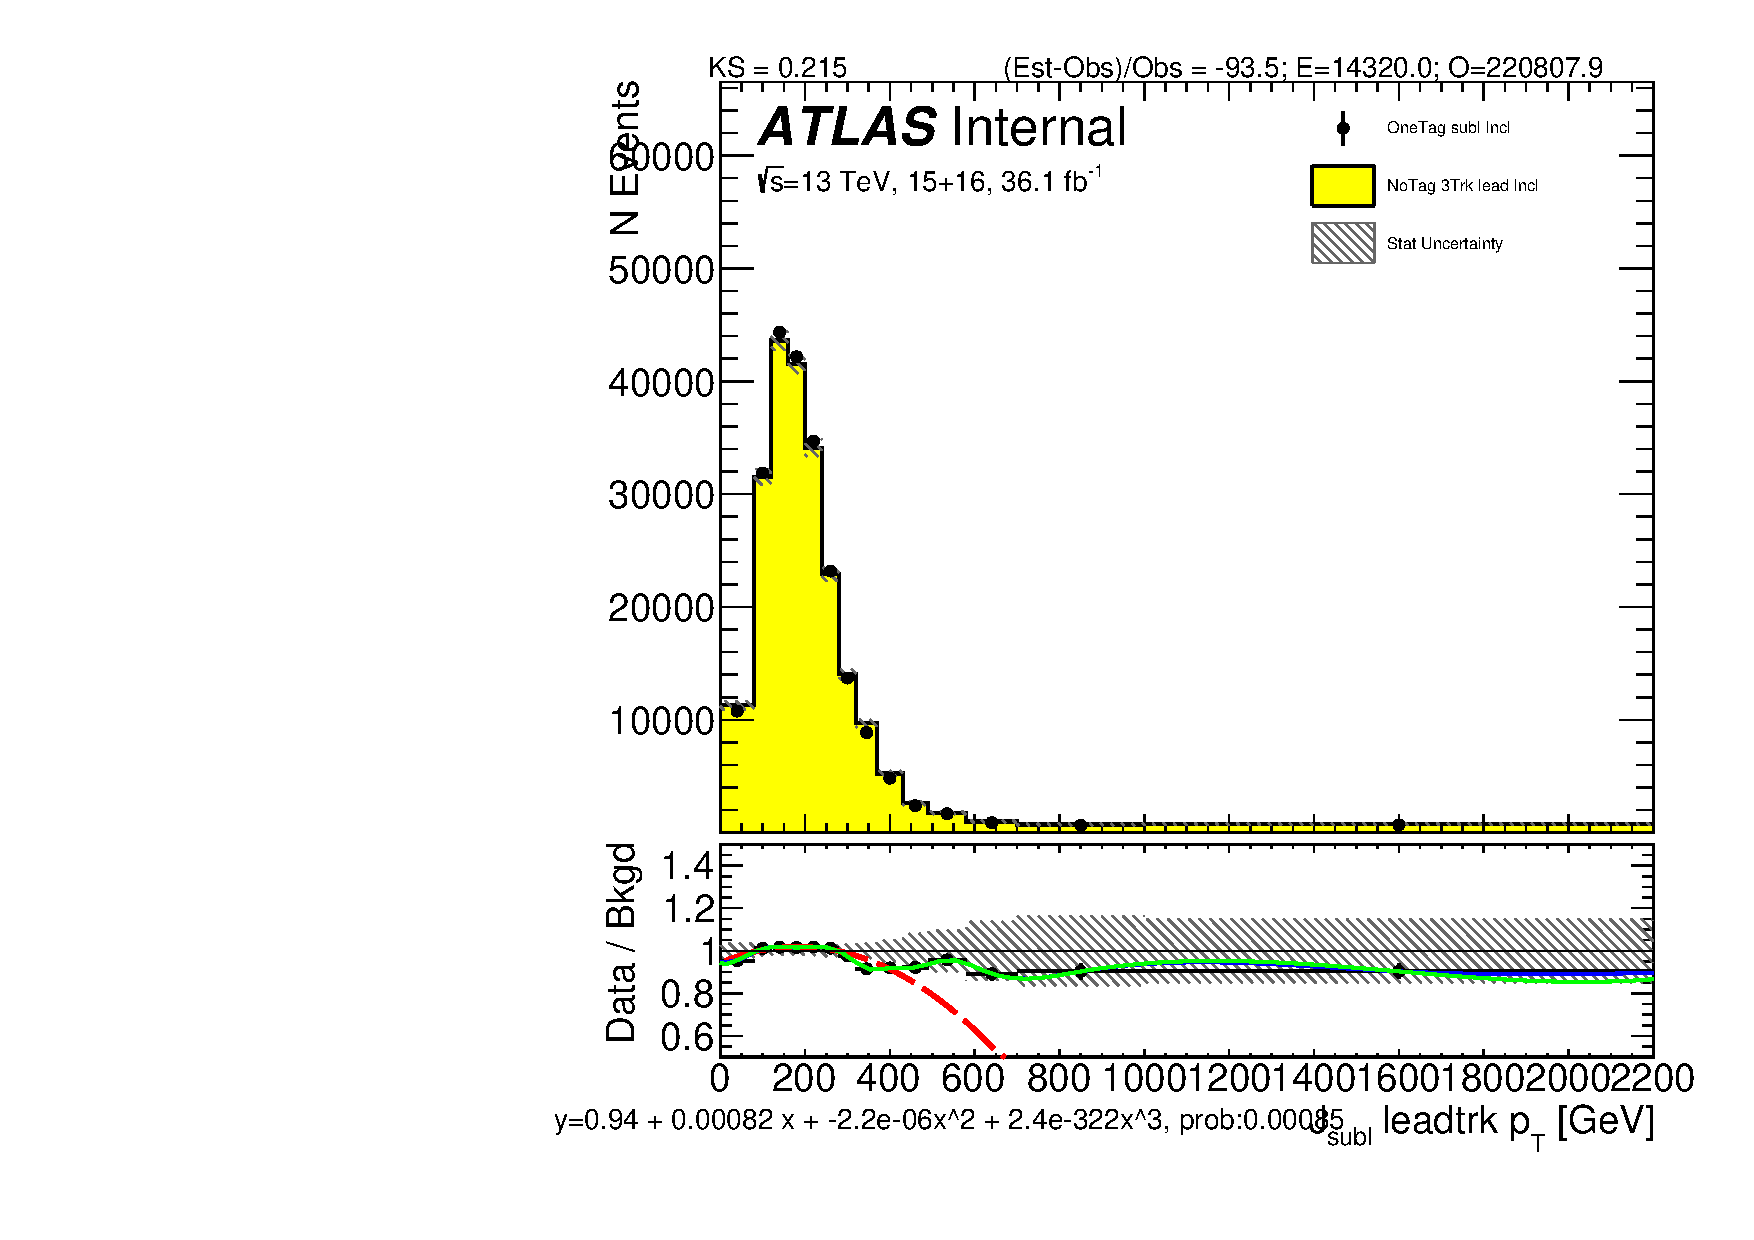
\includegraphics[width=0.32\textwidth,angle=-90]{figures/boosted/Reweight/Fits/Moriond_bkg_0_NoTag_3Trk_lead_Incl_sublHCand_trk0_Pt.pdf}
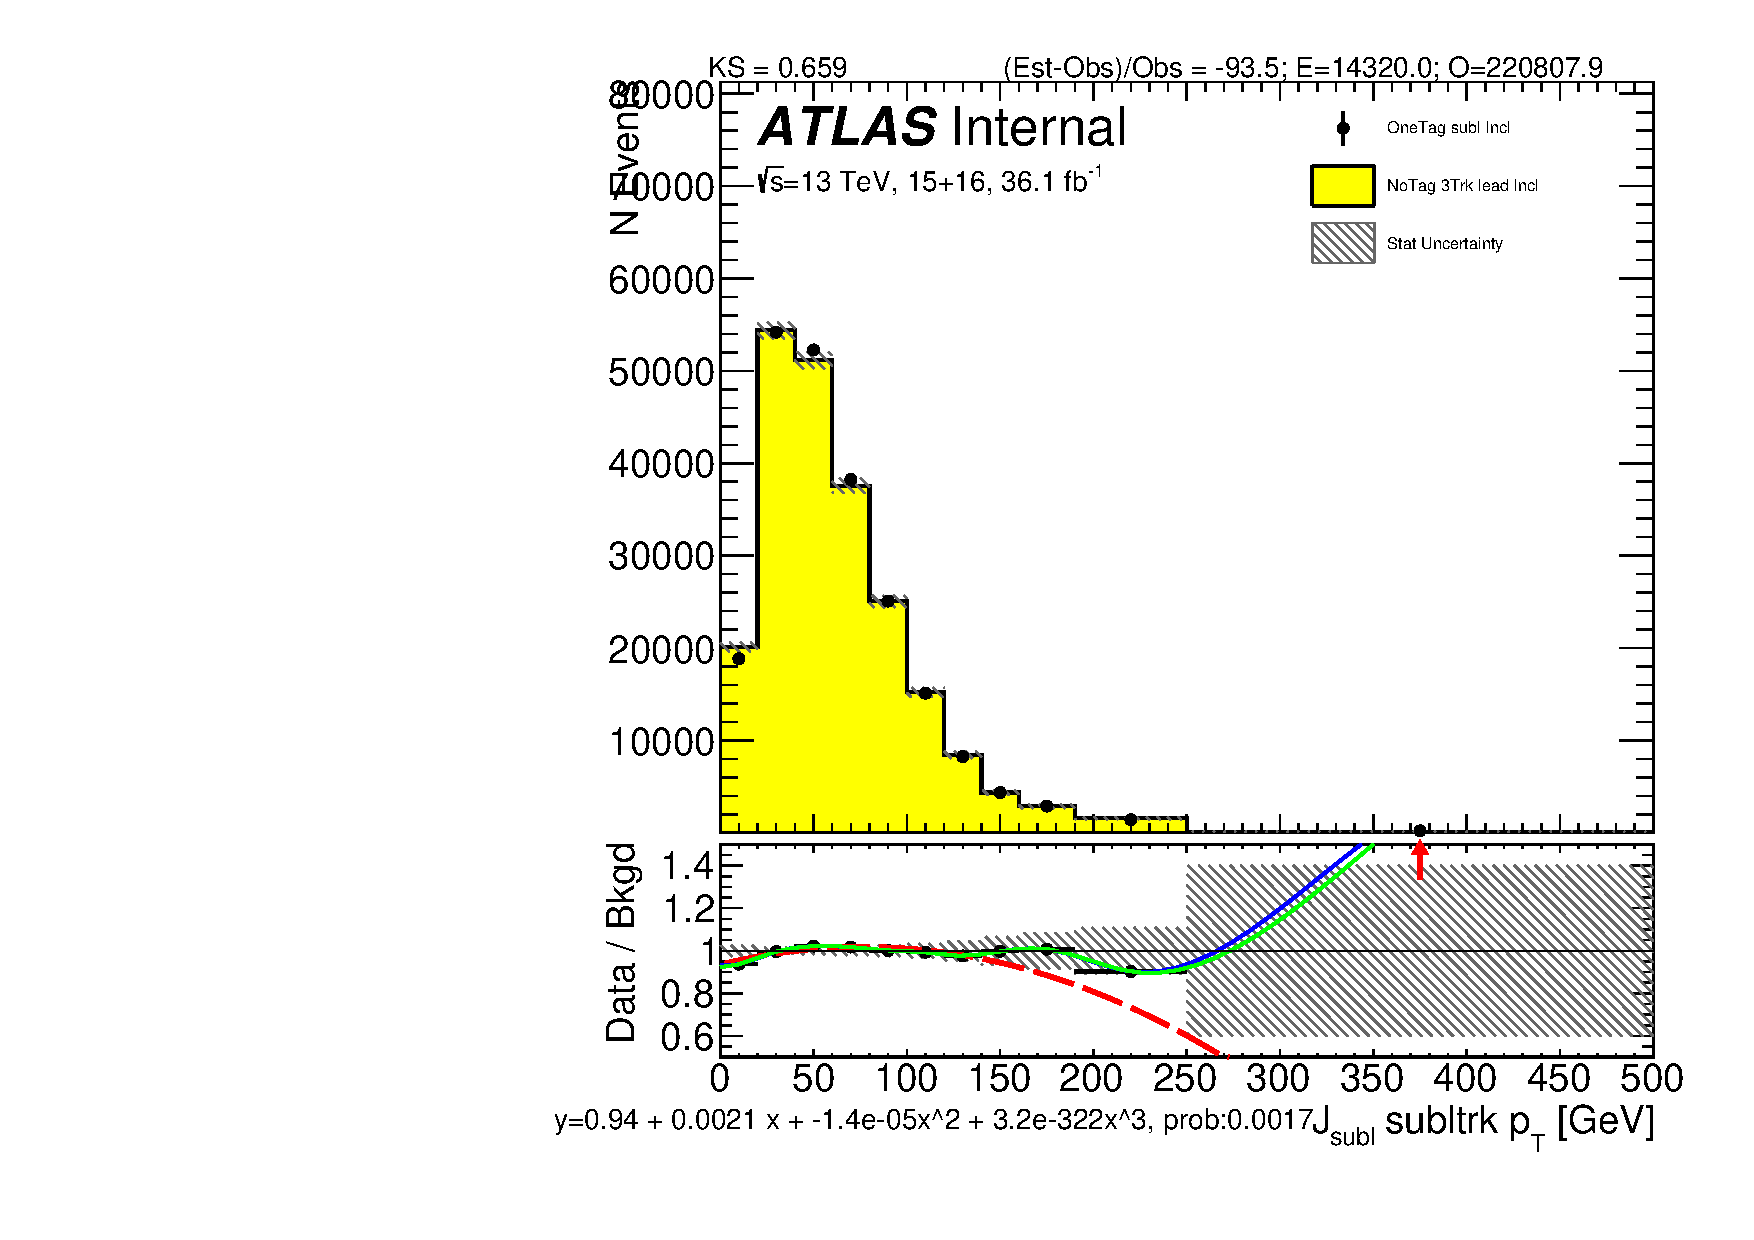
\includegraphics[width=0.32\textwidth,angle=-90]{figures/boosted/Reweight/Fits/Moriond_bkg_0_NoTag_3Trk_lead_Incl_sublHCand_trk1_Pt.pdf} \\
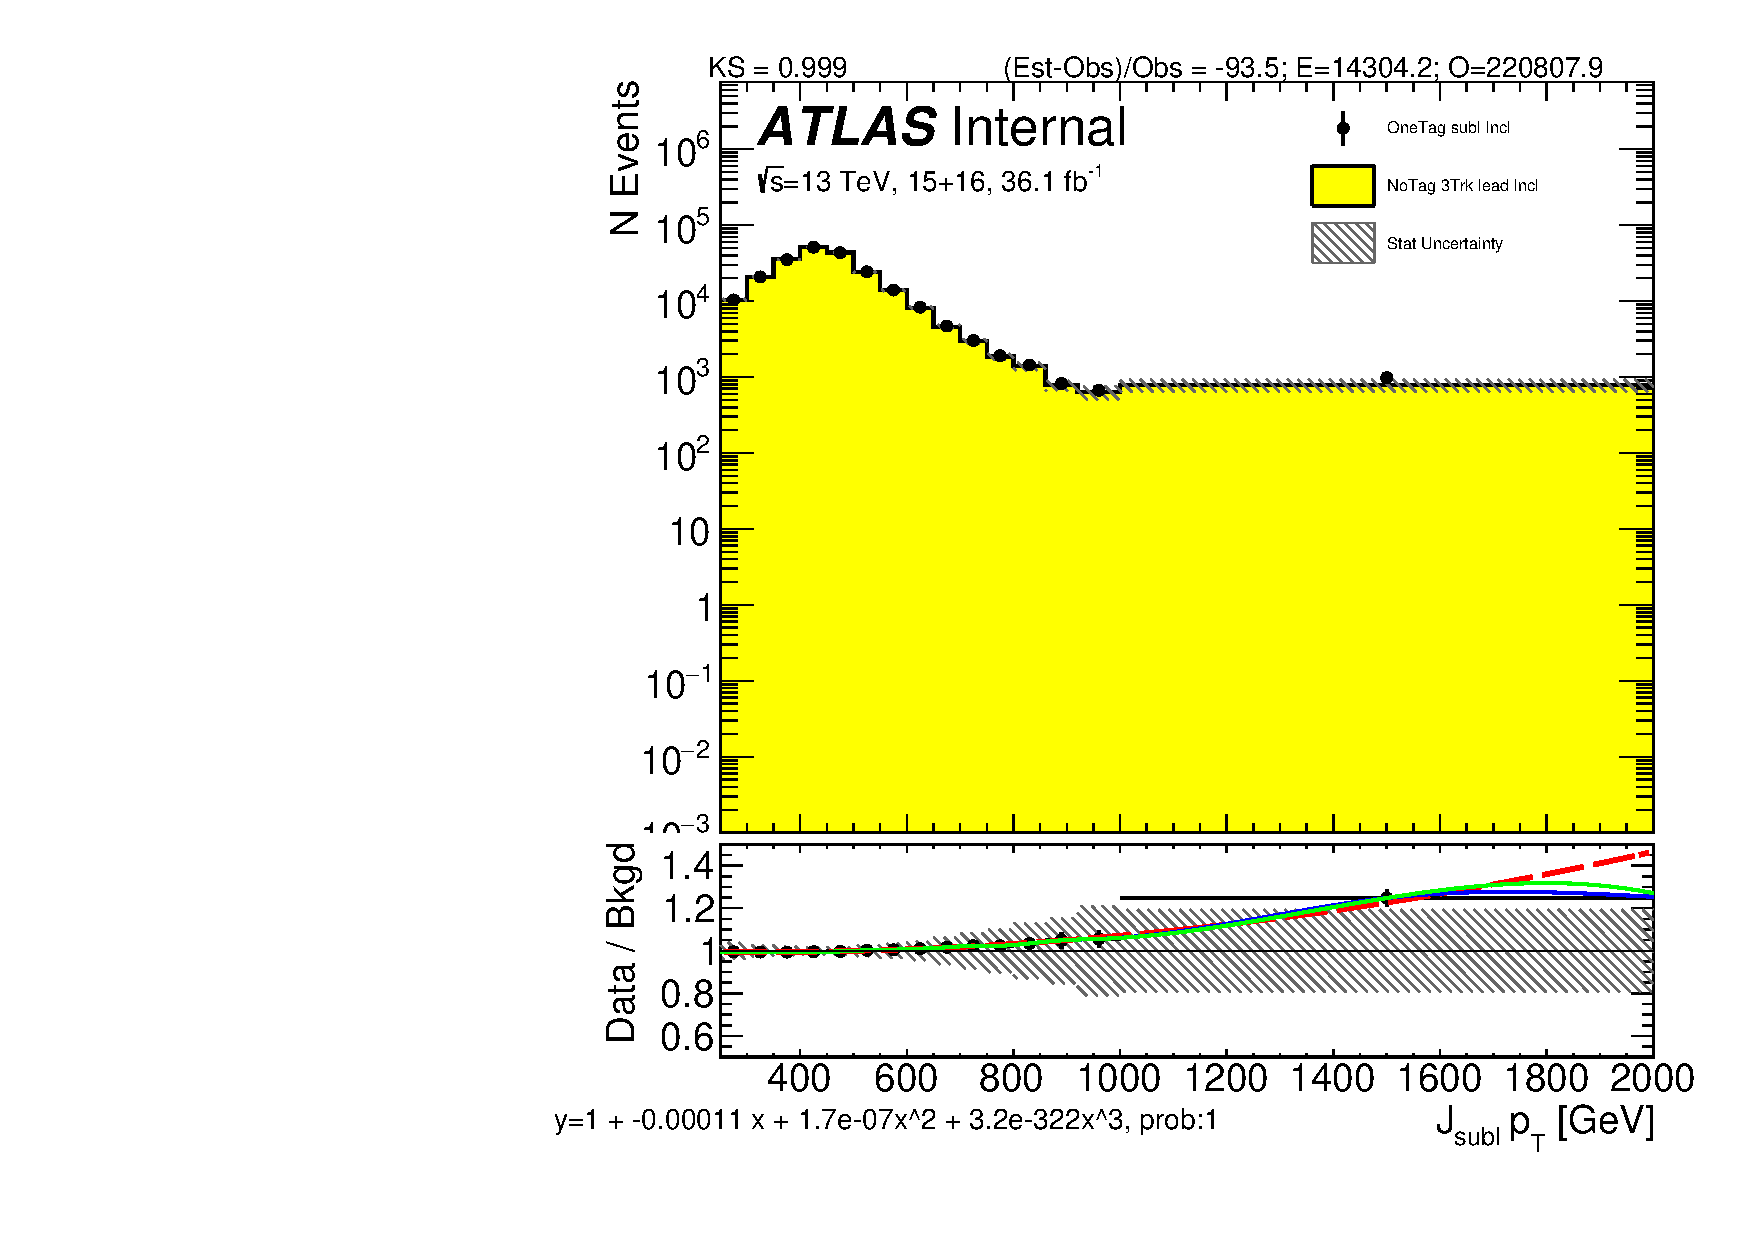
\includegraphics[width=0.32\textwidth,angle=-90]{figures/boosted/Reweight/Fits/Moriond_bkg_3_NoTag_3Trk_lead_Incl_sublHCand_Pt_m_1.pdf}
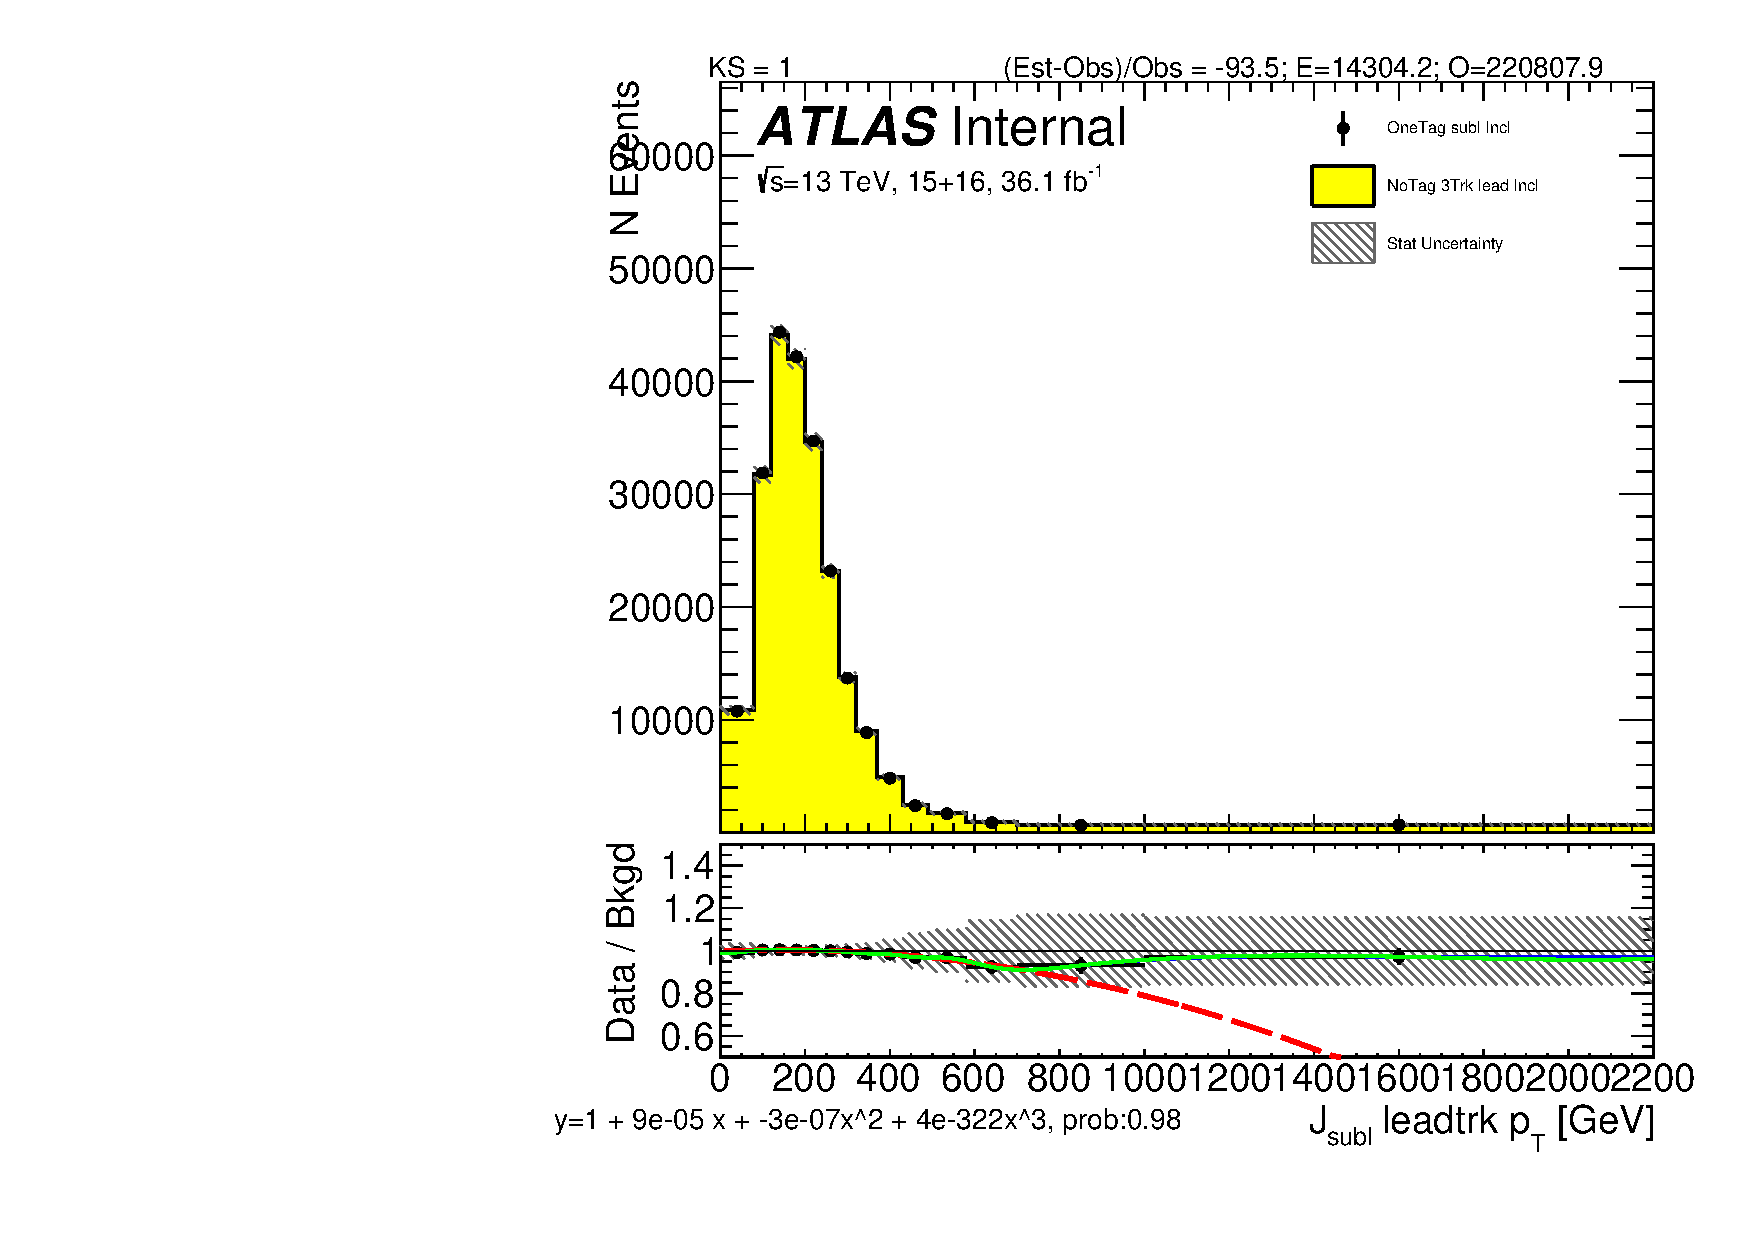
\includegraphics[width=0.32\textwidth,angle=-90]{figures/boosted/Reweight/Fits/Moriond_bkg_3_NoTag_3Trk_lead_Incl_sublHCand_trk0_Pt.pdf}
\includegraphics[width=0.32\textwidth,angle=-90]{figures/boosted/Reweight/Fits/Moriond_bkg_3_NoTag_3Trk_lead_Incl_sublHCand_trk1_Pt.pdf} \\
\includegraphics[width=0.32\textwidth,angle=-90]{figures/boosted/Reweight/Fits/Moriond_bkg_9_NoTag_3Trk_lead_Incl_sublHCand_Pt_m_1.pdf}
\includegraphics[width=0.32\textwidth,angle=-90]{figures/boosted/Reweight/Fits/Moriond_bkg_9_NoTag_3Trk_lead_Incl_sublHCand_trk0_Pt.pdf}
\includegraphics[width=0.32\textwidth,angle=-90]{figures/boosted/Reweight/Fits/Moriond_bkg_9_NoTag_3Trk_lead_Incl_sublHCand_trk1_Pt.pdf} \\
\caption{For 3$b$ background estimate: the fits to the ratio of the data in the 2$b$ category, of the sublleading Higgs candidate 2$b$-tagged events's subleading Higgs candidate distributions(black point), over the leading Higgs candidate 1$b$-tagged events's subleading Higgs candidate distributions(yellow). Distributions and fits to the estimated QCD background for large-$R$ jet $p_{T}$ (left),  the large-$R$ jet's leading trackjet $p_T$ (middle), and large-$R$ jet's subleading trackjet $p_T$ (right) are shown.  Figure are shown before reweighting (top row), after the first iteration(second row), after the fourth iteration(third row), and after the last iteration (bottow row). The green line is the spline extrapolation; and the red line is a polynomial fit.}
\label{fig:rw-3b-lead}
\end{center}
\end{figure*}

\begin{figure*}[htbp!]
\begin{center}
\includegraphics[width=0.32\textwidth,angle=-90]{figures/boosted/Reweight/Fits/Moriond_NoTag_3Trk_subl_Incl_leadHCand_Pt_m_1.pdf}
\includegraphics[width=0.32\textwidth,angle=-90]{figures/boosted/Reweight/Fits/Moriond_NoTag_3Trk_subl_Incl_leadHCand_trk0_Pt.pdf}
\includegraphics[width=0.32\textwidth,angle=-90]{figures/boosted/Reweight/Fits/Moriond_NoTag_3Trk_subl_Incl_leadHCand_trk1_Pt.pdf} \\
\includegraphics[width=0.32\textwidth,angle=-90]{figures/boosted/Reweight/Fits/Moriond_bkg_0_NoTag_3Trk_subl_Incl_leadHCand_Pt_m_1.pdf}
\includegraphics[width=0.32\textwidth,angle=-90]{figures/boosted/Reweight/Fits/Moriond_bkg_0_NoTag_3Trk_subl_Incl_leadHCand_trk0_Pt.pdf}
\includegraphics[width=0.32\textwidth,angle=-90]{figures/boosted/Reweight/Fits/Moriond_bkg_0_NoTag_3Trk_subl_Incl_leadHCand_trk1_Pt.pdf} \\
\includegraphics[width=0.32\textwidth,angle=-90]{figures/boosted/Reweight/Fits/Moriond_bkg_3_NoTag_3Trk_subl_Incl_leadHCand_Pt_m_1.pdf}
\includegraphics[width=0.32\textwidth,angle=-90]{figures/boosted/Reweight/Fits/Moriond_bkg_3_NoTag_3Trk_subl_Incl_leadHCand_trk0_Pt.pdf}
\includegraphics[width=0.32\textwidth,angle=-90]{figures/boosted/Reweight/Fits/Moriond_bkg_3_NoTag_3Trk_subl_Incl_leadHCand_trk1_Pt.pdf} \\
\includegraphics[width=0.32\textwidth,angle=-90]{figures/boosted/Reweight/Fits/Moriond_bkg_9_NoTag_3Trk_subl_Incl_leadHCand_Pt_m_1.pdf}
\includegraphics[width=0.32\textwidth,angle=-90]{figures/boosted/Reweight/Fits/Moriond_bkg_9_NoTag_3Trk_subl_Incl_leadHCand_trk0_Pt.pdf}
\includegraphics[width=0.32\textwidth,angle=-90]{figures/boosted/Reweight/Fits/Moriond_bkg_9_NoTag_3Trk_subl_Incl_leadHCand_trk1_Pt.pdf} \\
\caption{For 3$b$ background estimate: the fits to the ratio of the data in the 2$b$ category, of the leading Higgs candidate 2$b$-tagged events's leading Higgs candidate distributions(black point), over the sublleading Higgs candidate 1$b$-tagged events's leading Higgs candidate distributions(yellow). Distributions and fits to the estimated QCD background for large-$R$ jet $p_{T}$ (left),  the large-$R$ jet's leading trackjet $p_T$ (middle), and large-$R$ jet's subleading trackjet $p_T$ (right) are shown.  Figure are shown before reweighting (top row), after the first iteration(second row), after the fourth iteration(third row), and after the last iteration (bottow row). The green line is the spline extrapolation; and the red line is a polynomial fit.}
\label{fig:rw-3b-subl}
\end{center}
\end{figure*}

\begin{figure*}[htbp!]
\begin{center}
\includegraphics[width=0.32\textwidth,angle=-90]{figures/boosted/Reweight/Fits/Moriond_NoTag_4Trk_lead_Incl_sublHCand_Pt_m_1.pdf}
\includegraphics[width=0.32\textwidth,angle=-90]{figures/boosted/Reweight/Fits/Moriond_NoTag_4Trk_lead_Incl_sublHCand_trk0_Pt.pdf}
\includegraphics[width=0.32\textwidth,angle=-90]{figures/boosted/Reweight/Fits/Moriond_NoTag_4Trk_lead_Incl_sublHCand_trk1_Pt.pdf} \\
\includegraphics[width=0.32\textwidth,angle=-90]{figures/boosted/Reweight/Fits/Moriond_bkg_0_NoTag_4Trk_lead_Incl_sublHCand_Pt_m_1.pdf}
\includegraphics[width=0.32\textwidth,angle=-90]{figures/boosted/Reweight/Fits/Moriond_bkg_0_NoTag_4Trk_lead_Incl_sublHCand_trk0_Pt.pdf}
\includegraphics[width=0.32\textwidth,angle=-90]{figures/boosted/Reweight/Fits/Moriond_bkg_0_NoTag_4Trk_lead_Incl_sublHCand_trk1_Pt.pdf} \\
\includegraphics[width=0.32\textwidth,angle=-90]{figures/boosted/Reweight/Fits/Moriond_bkg_3_NoTag_4Trk_lead_Incl_sublHCand_Pt_m_1.pdf}
\includegraphics[width=0.32\textwidth,angle=-90]{figures/boosted/Reweight/Fits/Moriond_bkg_3_NoTag_4Trk_lead_Incl_sublHCand_trk0_Pt.pdf}
\includegraphics[width=0.32\textwidth,angle=-90]{figures/boosted/Reweight/Fits/Moriond_bkg_3_NoTag_4Trk_lead_Incl_sublHCand_trk1_Pt.pdf} \\
\includegraphics[width=0.32\textwidth,angle=-90]{figures/boosted/Reweight/Fits/Moriond_bkg_9_NoTag_4Trk_lead_Incl_sublHCand_Pt_m_1.pdf}
\includegraphics[width=0.32\textwidth,angle=-90]{figures/boosted/Reweight/Fits/Moriond_bkg_9_NoTag_4Trk_lead_Incl_sublHCand_trk0_Pt.pdf}
\includegraphics[width=0.32\textwidth,angle=-90]{figures/boosted/Reweight/Fits/Moriond_bkg_9_NoTag_4Trk_lead_Incl_sublHCand_trk1_Pt.pdf} \\
\caption{For 4$b$ background estimate: the fits to the ratio of the data in the 2$b$ category, of the sublleading Higgs candidate 2$b$-tagged events's subleading Higgs candidate distributions(black point), over the leading Higgs candidate 2$b$-tagged events's subleading Higgs candidate distributions(yellow). Distributions and fits to the estimated QCD background for large-$R$ jet $p_{T}$ (left),  the large-$R$ jet's leading trackjet $p_T$ (middle), and large-$R$ jet's subleading trackjet $p_T$ (right) are shown.  Figure are shown before reweighting (top row), after the first iteration(second row), after the fourth iteration(third row), and after the last iteration (bottow row). The green line is the spline extrapolation; and the red line is a polynomial fit.}
\label{fig:rw-4b-lead}
\end{center}
\end{figure*}

\begin{figure*}[htbp!]
\begin{center}
\includegraphics[width=0.32\textwidth,angle=-90]{figures/boosted/Reweight/Fits/Moriond_NoTag_4Trk_subl_Incl_leadHCand_Pt_m_1.pdf}
\includegraphics[width=0.32\textwidth,angle=-90]{figures/boosted/Reweight/Fits/Moriond_NoTag_4Trk_subl_Incl_leadHCand_trk0_Pt.pdf}
\includegraphics[width=0.32\textwidth,angle=-90]{figures/boosted/Reweight/Fits/Moriond_NoTag_4Trk_subl_Incl_leadHCand_trk1_Pt.pdf} \\
\includegraphics[width=0.32\textwidth,angle=-90]{figures/boosted/Reweight/Fits/Moriond_bkg_0_NoTag_4Trk_subl_Incl_leadHCand_Pt_m_1.pdf}
\includegraphics[width=0.32\textwidth,angle=-90]{figures/boosted/Reweight/Fits/Moriond_bkg_0_NoTag_4Trk_subl_Incl_leadHCand_trk0_Pt.pdf}
\includegraphics[width=0.32\textwidth,angle=-90]{figures/boosted/Reweight/Fits/Moriond_bkg_0_NoTag_4Trk_subl_Incl_leadHCand_trk1_Pt.pdf} \\
\includegraphics[width=0.32\textwidth,angle=-90]{figures/boosted/Reweight/Fits/Moriond_bkg_3_NoTag_4Trk_subl_Incl_leadHCand_Pt_m_1.pdf}
\includegraphics[width=0.32\textwidth,angle=-90]{figures/boosted/Reweight/Fits/Moriond_bkg_3_NoTag_4Trk_subl_Incl_leadHCand_trk0_Pt.pdf}
\includegraphics[width=0.32\textwidth,angle=-90]{figures/boosted/Reweight/Fits/Moriond_bkg_3_NoTag_4Trk_subl_Incl_leadHCand_trk1_Pt.pdf} \\
\includegraphics[width=0.32\textwidth,angle=-90]{figures/boosted/Reweight/Fits/Moriond_bkg_9_NoTag_4Trk_subl_Incl_leadHCand_Pt_m_1.pdf}
\includegraphics[width=0.32\textwidth,angle=-90]{figures/boosted/Reweight/Fits/Moriond_bkg_9_NoTag_4Trk_subl_Incl_leadHCand_trk0_Pt.pdf}
\includegraphics[width=0.32\textwidth,angle=-90]{figures/boosted/Reweight/Fits/Moriond_bkg_9_NoTag_4Trk_subl_Incl_leadHCand_trk1_Pt.pdf} \\
\caption{For 4$b$ background estimate: the fits to the ratio of the data in the 2$b$ category, of the leading Higgs candidate 2$b$-tagged events's leading Higgs candidate distributions(black point), over the sublleading Higgs candidate 2$b$-tagged events's leading Higgs candidate distributions(yellow). Distributions and fits to the estimated QCD background for large-$R$ jet $p_{T}$ (left),  the large-$R$ jet's leading trackjet $p_T$ (middle), and large-$R$ jet's subleading trackjet $p_T$ (right) are shown.  Figure are shown before reweighting (top row), after the first iteration(second row), after the fourth iteration(third row), and after the last iteration (bottow row). The green line is the spline extrapolation; and the red line is a polynomial fit.}
\label{fig:rw-4b-subl}
\end{center}
\end{figure*}


\pagebreak{}
%%%%%%%%%%%%%%%%%%%%%%%%%%%
\subsubsection{Reweighting Results Comparison in Sideband and Control Region}
\label{sec:boosted-Reweight-compare}

%%\paragraph{}
A comparison of the Sideband shapes before and after reweighting for 2$b$s, 3$b$ and 4$b$ can be seen in Figures~\ref{fig:rw-2bs-comp-sb},~\ref{fig:rw-3b-comp-sb}, and ~\ref{fig:rw-4b-comp-sb}. Also, a comparison of the Control Region shapes before and after reweighting for 2$b$s, 3$b$ and 4$b$ can be seen in Figures~\ref{fig:rw-2bs-comp-cr},~\ref{fig:rw-3b-comp-cr}, and ~\ref{fig:rw-4b-comp-cr}. In almost all cases, both the reweighted/non-reweighted prediction agrees fairly well with the data, and the reweighted plots' KS score improved from non-reweighted distributions. 

%%%%%%%%%%%%%%%%%%%%%%%%%%%
\begin{figure*}[htbp!]
\begin{center}
\includegraphics[width=0.31\textwidth,angle=-90]{figures/boosted/Prereweight/Moriond_TwoTag_split_Sideband_mHH_l_1.pdf}
\includegraphics[width=0.31\textwidth,angle=-90]{figures/boosted/Sideband/b77_TwoTag_split_Sideband_mHH_l_1.pdf}\\
\includegraphics[width=0.31\textwidth,angle=-90]{figures/boosted/Prereweight/Moriond_TwoTag_split_Sideband_leadHCand_Pt_m.pdf}
\includegraphics[width=0.31\textwidth,angle=-90]{figures/boosted/Sideband/b77_TwoTag_split_Sideband_leadHCand_Pt_m.pdf}\\
\includegraphics[width=0.31\textwidth,angle=-90]{figures/boosted/Prereweight/Moriond_TwoTag_split_Sideband_leadHCand_trk0_Pt.pdf}
\includegraphics[width=0.31\textwidth,angle=-90]{figures/boosted/Sideband/b77_TwoTag_split_Sideband_leadHCand_trk0_Pt.pdf}\\
\includegraphics[width=0.31\textwidth,angle=-90]{figures/boosted/Prereweight/Moriond_TwoTag_split_Sideband_sublHCand_trk0_Pt.pdf}
\includegraphics[width=0.31\textwidth,angle=-90]{figures/boosted/Sideband/b77_TwoTag_split_Sideband_sublHCand_trk0_Pt.pdf}\\
\caption{Reweighted 2$b$s Sideband region predictions comaprison. Top row is the dijet Mass, second row is leading large-$R$ jet $p_{T}$, third row is the leading large-$R$ jet's leading trackjet $p_T$ and the last row subleading large-$R$ jet's leading trackjet $p_T$. On the left are the distributions before reweighting, and on the right are the distributions after reweighting.}
\label{fig:rw-2bs-comp-sb}
\end{center}
\end{figure*}


\begin{figure*}[htbp!]
\begin{center}
\includegraphics[width=0.31\textwidth,angle=-90]{figures/boosted/Prereweight/Moriond_ThreeTag_Sideband_mHH_l_1.pdf}
\includegraphics[width=0.31\textwidth,angle=-90]{figures/boosted/Sideband/b77_ThreeTag_Sideband_mHH_l_1.pdf}\\
\includegraphics[width=0.31\textwidth,angle=-90]{figures/boosted/Prereweight/Moriond_ThreeTag_Sideband_leadHCand_Pt_m.pdf}
\includegraphics[width=0.31\textwidth,angle=-90]{figures/boosted/Sideband/b77_ThreeTag_Sideband_leadHCand_Pt_m.pdf}\\
\includegraphics[width=0.31\textwidth,angle=-90]{figures/boosted/Prereweight/Moriond_ThreeTag_Sideband_leadHCand_trk0_Pt.pdf}
\includegraphics[width=0.31\textwidth,angle=-90]{figures/boosted/Sideband/b77_ThreeTag_Sideband_leadHCand_trk0_Pt.pdf}\\
\includegraphics[width=0.31\textwidth,angle=-90]{figures/boosted/Prereweight/Moriond_ThreeTag_Sideband_sublHCand_trk0_Pt.pdf}
\includegraphics[width=0.31\textwidth,angle=-90]{figures/boosted/Sideband/b77_ThreeTag_Sideband_sublHCand_trk0_Pt.pdf}\\
\caption{Reweighted 3$b$ Sideband region predictions comaprison. Top row is the dijet Mass, second row is leading large-$R$ jet $p_{T}$, third row is the leading large-$R$ jet's leading trackjet $p_T$ and the last row subleading large-$R$ jet's leading trackjet $p_T$. On the left are the distributions before reweighting, and on the right are the distributions after reweighting.}
\label{fig:rw-3b-comp-sb}
\end{center}
\end{figure*}


\begin{figure*}[htbp!]
\begin{center}
\includegraphics[width=0.31\textwidth,angle=-90]{figures/boosted/Prereweight/Moriond_FourTag_Sideband_mHH_l_1.pdf}
\includegraphics[width=0.31\textwidth,angle=-90]{figures/boosted/Sideband/b77_FourTag_Sideband_mHH_l_1.pdf}\\
\includegraphics[width=0.31\textwidth,angle=-90]{figures/boosted/Prereweight/Moriond_FourTag_Sideband_leadHCand_Pt_m.pdf}
\includegraphics[width=0.31\textwidth,angle=-90]{figures/boosted/Sideband/b77_FourTag_Sideband_leadHCand_Pt_m.pdf}\\
\includegraphics[width=0.31\textwidth,angle=-90]{figures/boosted/Prereweight/Moriond_FourTag_Sideband_leadHCand_trk0_Pt.pdf}
\includegraphics[width=0.31\textwidth,angle=-90]{figures/boosted/Sideband/b77_FourTag_Sideband_leadHCand_trk0_Pt.pdf}\\
\includegraphics[width=0.31\textwidth,angle=-90]{figures/boosted/Prereweight/Moriond_FourTag_Sideband_sublHCand_trk0_Pt.pdf}
\includegraphics[width=0.31\textwidth,angle=-90]{figures/boosted/Sideband/b77_FourTag_Sideband_sublHCand_trk0_Pt.pdf}\\
\caption{Reweighted 4$b$ Sideband region predictions comaprison. Top row is the dijet Mass, second row is leading large-$R$ jet $p_{T}$, third row is the leading large-$R$ jet's leading trackjet $p_T$ and the last row subleading large-$R$ jet's leading trackjet $p_T$. On the left are the distributions before reweighting, and on the right are the distributions after reweighting.}
\label{fig:rw-4b-comp-sb}
\end{center}
\end{figure*}



%%%%%%%%%%%%%%%%%%%%%%%%%%%
\begin{figure*}[htbp!]
\begin{center}
\includegraphics[width=0.31\textwidth,angle=-90]{figures/boosted/Prereweight/Moriond_TwoTag_split_Control_mHH_l_1.pdf}
\includegraphics[width=0.31\textwidth,angle=-90]{figures/boosted/Control/b77_TwoTag_split_Control_mHH_l_1.pdf}\\
\includegraphics[width=0.31\textwidth,angle=-90]{figures/boosted/Prereweight/Moriond_TwoTag_split_Control_leadHCand_Pt_m.pdf}
\includegraphics[width=0.31\textwidth,angle=-90]{figures/boosted/Control/b77_TwoTag_split_Control_leadHCand_Pt_m.pdf}\\
\includegraphics[width=0.31\textwidth,angle=-90]{figures/boosted/Prereweight/Moriond_TwoTag_split_Control_leadHCand_trk0_Pt.pdf}
\includegraphics[width=0.31\textwidth,angle=-90]{figures/boosted/Control/b77_TwoTag_split_Control_leadHCand_trk0_Pt.pdf}\\
\includegraphics[width=0.31\textwidth,angle=-90]{figures/boosted/Prereweight/Moriond_TwoTag_split_Control_sublHCand_trk0_Pt.pdf}
\includegraphics[width=0.31\textwidth,angle=-90]{figures/boosted/Control/b77_TwoTag_split_Control_sublHCand_trk0_Pt.pdf}\\
\caption{Reweighted 2$b$s Control region predictions comaprison. Top row is the dijet Mass, second row is leading large-$R$ jet $p_{T}$, third row is the leading large-$R$ jet's leading trackjet $p_T$ and the last row subleading large-$R$ jet's leading trackjet $p_T$. On the left are the distributions before reweighting, and on the right are the distributions after reweighting.}
\label{fig:rw-2bs-comp-cr}
\end{center}
\end{figure*}


\begin{figure*}[htbp!]
\begin{center}
\includegraphics[width=0.31\textwidth,angle=-90]{figures/boosted/Prereweight/Moriond_ThreeTag_Control_mHH_l_1.pdf}
\includegraphics[width=0.31\textwidth,angle=-90]{figures/boosted/Control/b77_ThreeTag_Control_mHH_l_1.pdf}\\
\includegraphics[width=0.31\textwidth,angle=-90]{figures/boosted/Prereweight/Moriond_ThreeTag_Control_leadHCand_Pt_m.pdf}
\includegraphics[width=0.31\textwidth,angle=-90]{figures/boosted/Control/b77_ThreeTag_Control_leadHCand_Pt_m.pdf}\\
\includegraphics[width=0.31\textwidth,angle=-90]{figures/boosted/Prereweight/Moriond_ThreeTag_Control_leadHCand_trk0_Pt.pdf}
\includegraphics[width=0.31\textwidth,angle=-90]{figures/boosted/Control/b77_ThreeTag_Control_leadHCand_trk0_Pt.pdf}\\
\includegraphics[width=0.31\textwidth,angle=-90]{figures/boosted/Prereweight/Moriond_ThreeTag_Control_sublHCand_trk0_Pt.pdf}
\includegraphics[width=0.31\textwidth,angle=-90]{figures/boosted/Control/b77_ThreeTag_Control_sublHCand_trk0_Pt.pdf}\\
\caption{Reweighted 3$b$ Control region predictions comaprison. Top row is the dijet Mass, second row is leading large-$R$ jet $p_{T}$, third row is the leading large-$R$ jet's leading trackjet $p_T$ and the last row subleading large-$R$ jet's leading trackjet $p_T$. On the left are the distributions before reweighting, and on the right are the distributions after reweighting.}
\label{fig:rw-3b-comp-cr}
\end{center}
\end{figure*}


\begin{figure*}[htbp!]
\begin{center}
\includegraphics[width=0.31\textwidth,angle=-90]{figures/boosted/Prereweight/Moriond_FourTag_Control_mHH_l_1.pdf}
\includegraphics[width=0.31\textwidth,angle=-90]{figures/boosted/Control/b77_FourTag_Control_mHH_l_1.pdf}\\
\includegraphics[width=0.31\textwidth,angle=-90]{figures/boosted/Prereweight/Moriond_FourTag_Control_leadHCand_Pt_m.pdf}
\includegraphics[width=0.31\textwidth,angle=-90]{figures/boosted/Control/b77_FourTag_Control_leadHCand_Pt_m.pdf}\\
\includegraphics[width=0.31\textwidth,angle=-90]{figures/boosted/Prereweight/Moriond_FourTag_Control_leadHCand_trk0_Pt.pdf}
\includegraphics[width=0.31\textwidth,angle=-90]{figures/boosted/Control/b77_FourTag_Control_leadHCand_trk0_Pt.pdf}\\
\includegraphics[width=0.31\textwidth,angle=-90]{figures/boosted/Prereweight/Moriond_FourTag_Control_sublHCand_trk0_Pt.pdf}
\includegraphics[width=0.31\textwidth,angle=-90]{figures/boosted/Control/b77_FourTag_Control_sublHCand_trk0_Pt.pdf}\\
\caption{Reweighted 4$b$ Control region predictions comaprison. Top row is the dijet Mass, second row is leading large-$R$ jet $p_{T}$, third row is the leading large-$R$ jet's leading trackjet $p_T$ and the last row subleading large-$R$ jet's leading trackjet $p_T$. On the left are the distributions before reweighting, and on the right are the distributions after reweighting.}
\label{fig:rw-4b-comp-cr}
\end{center}
\end{figure*}

\clearpage


%%%%%%%%%%%%%%%%%%%%%%%%%%%%%%%%%%%%%%%%%%%%%%%%%%%%%%%%%%%%%%%%%%%%%%%
%%%%%%%%%%%%%%%%%%%%%%%%%%%%%%%%%%%%%%%%%%%%%%%%%%%%%%%%%%%%%%%%%%%%%%%
%%%  SB plots
%%%%%%%%%%%%%%%%%%%%%%%%%%%%%%%%%%%%%%%%%%%%%%%%%%%%%%%%%%%%%%%%%%%%%%%
%%%%%%%%%%%%%%%%%%%%%%%%%%%%%%%%%%%%%%%%%%%%%%%%%%%%%%%%%%%%%%%%%%%%%%%
\subsection{Predictions in the sideband region (SB)}
\label{sec:boosted-sb}

\paragraph{}
This section shows comparisons of data with the prediction of QCD multi-jets and \ttbar in the sideband region (SB), which is identical to the signal region (SR) except the large-$R$ jets are required to have masses far from the Higgs mass. The definition of the sideband and control regions is discussed in Section~\ref{sec:boosted-SBCR}. The predicted and observed event yields are summarized in Tables~\ref{tab:yields4b} and~\ref{tab:yields3b}.

\paragraph{}
Figures~\ref{fig:boosted-4b-sideband-ak10-lead}, \ref{fig:boosted-4b-sideband-ak10-subl}, \ref{fig:boosted-4b-sideband-ak2},  and \ref{fig:boosted-4b-sideband-ak10-system} show predictions of various kinematics of the large-$R$ jets and their associated track jets in the 4$b$ selection. The predicted normalization agrees perfectly by construction, but the shapes are a feature of the prediction. The quality of the prediction is generally good, and no clear systematic biases are observed.


\paragraph{}
Figures~\ref{fig:boosted-3b-sideband-ak10-lead}, \ref{fig:boosted-3b-sideband-ak10-subl}, \ref{fig:boosted-3b-sideband-ak2},  and \ref{fig:boosted-3b-sideband-ak10-system} show predictions of various kinematics of the large-$R$ jets and their associated track jets in the 3$b$ selection. The predicted normalization agrees perfectly by construction, but the shapes are a feature of the prediction. The quality of the prediction is generally good, and no clear systematic biases are observed.


\paragraph{}
Figures~\ref{fig:boosted-2bs-sideband-ak10-lead}, \ref{fig:boosted-2bs-sideband-ak10-subl}, \ref{fig:boosted-2bs-sideband-ak2},  and \ref{fig:boosted-2bs-sideband-ak10-system} show predictions of various kinematics of the large-$R$ jets and their associated track jets in the 2$bs$ selection. The predicted normalization agrees perfectly by construction, but the shapes are a feature of the prediction. The quality of the prediction is generally good, and no clear systematic biases are observed.

% \paragraph{}
% No corrections to the prediction in the SB are obviously needed. One hypothesis for this behavior is that the large-$R$ jet trigger used in the boosted category has negligible dependence on the $b$-tag multiplicity of the event, hence extrapolating from the $1/2b$ region to the 2,3,4$b$ region is straightforward. On the other hand, the resolved analysis relies on $b$-jet triggers, which can have dependence on the $b$-tag multiplicity.

\begin{figure*}[htbp!]
\begin{center}
\includegraphics[angle=270, width=0.45\textwidth]{./figures/boosted/Sideband/b77_FourTag_Sideband_leadHCand_Pt_m_1.pdf}
\includegraphics[angle=270, width=0.45\textwidth]{./figures/boosted/Sideband/b77_FourTag_Sideband_leadHCand_Mass_s.pdf}\\
\includegraphics[angle=270, width=0.45\textwidth]{./figures/boosted/Sideband/b77_FourTag_Sideband_leadHCand_Eta.pdf}
\includegraphics[angle=270, width=0.45\textwidth]{./figures/boosted/Sideband/b77_FourTag_Sideband_leadHCand_Phi.pdf}
  \caption{Kinematics of the lead large-$R$ jet in data and prediction in the sideband region after requiring 4 $b$-tags. The normalization agrees by construction, and the shapes are a feature of the prediction.}
  \label{fig:boosted-4b-sideband-ak10-lead}
\end{center}
\end{figure*}

\begin{figure*}[htbp!]
\begin{center}
\includegraphics[angle=270, width=0.45\textwidth]{./figures/boosted/Sideband/b77_FourTag_Sideband_sublHCand_Pt_m_1.pdf}
\includegraphics[angle=270, width=0.45\textwidth]{./figures/boosted/Sideband/b77_FourTag_Sideband_sublHCand_Mass_s.pdf}\\
\includegraphics[angle=270, width=0.45\textwidth]{./figures/boosted/Sideband/b77_FourTag_Sideband_sublHCand_Eta.pdf}
\includegraphics[angle=270, width=0.45\textwidth]{./figures/boosted/Sideband/b77_FourTag_Sideband_sublHCand_Phi.pdf}
  \caption{Kinematics of the sub-lead large-$R$ jet in data and prediction in the sideband region after requiring 4 $b$-tags. The normalization agrees by construction, and the shapes are a feature of the prediction.}
  \label{fig:boosted-4b-sideband-ak10-subl}
\end{center}
\end{figure*}

\begin{figure*}[htbp!]
\begin{center}
\includegraphics[angle=270, width=0.45\textwidth]{./figures/boosted/Sideband/b77_FourTag_Sideband_leadHCand_trk0_Pt.pdf}
\includegraphics[angle=270, width=0.45\textwidth]{./figures/boosted/Sideband/b77_FourTag_Sideband_leadHCand_trk1_Pt.pdf}\\
\includegraphics[angle=270, width=0.45\textwidth]{./figures/boosted/Sideband/b77_FourTag_Sideband_sublHCand_trk0_Pt.pdf}
\includegraphics[angle=270, width=0.45\textwidth]{./figures/boosted/Sideband/b77_FourTag_Sideband_sublHCand_trk1_Pt.pdf}\\
\includegraphics[angle=270, width=0.45\textwidth]{./figures/boosted/Sideband/b77_FourTag_Sideband_leadHCand_trk_dr.pdf}
\includegraphics[angle=270, width=0.45\textwidth]{./figures/boosted/Sideband/b77_FourTag_Sideband_sublHCand_trk_dr.pdf}
  \caption{First two rows show the kinematics of the lead (left) and sub-lead (right) small-$R$ track jets associated to the lead (first-row) and sub-lead (second-row) large-$R$ jet in data and prediction in the sideband region after requiring 4 $b$-tags. Third row shows the $\Delta R$ between two leading small-$R$ track-jets associated to the leading (left) and sub-leading (right) large-$R$ jet. The normalization agrees by construction, and the shapes are a feature of the prediction. }
  \label{fig:boosted-4b-sideband-ak2}
\end{center}
\end{figure*}


\begin{figure*}[htbp!]
\begin{center}
\includegraphics[angle=270, width=0.45\textwidth]{./figures/boosted/Sideband/b77_FourTag_Sideband_mHH_l_1.pdf}
\includegraphics[angle=270, width=0.45\textwidth]{./figures/boosted/Sideband/b77_FourTag_Sideband_hCandDr.pdf}\\
\includegraphics[angle=270, width=0.45\textwidth]{./figures/boosted/Sideband/b77_FourTag_Sideband_hCandDeta.pdf}
\includegraphics[angle=270, width=0.45\textwidth]{./figures/boosted/Sideband/b77_FourTag_Sideband_hCandDphi.pdf}
  \caption{Kinematics of the large-$R$ jet system in data and prediction in the sideband region after requiring 4 $b$-tags. The normalization agrees by construction, and the shapes are a feature of the prediction. }
  \label{fig:boosted-4b-sideband-ak10-system}
\end{center}
\end{figure*}

\clearpage

\begin{figure*}[htbp!]
\begin{center}
\includegraphics[angle=270, width=0.45\textwidth]{./figures/boosted/Sideband/b77_ThreeTag_Sideband_leadHCand_Pt_m_1.pdf}
\includegraphics[angle=270, width=0.45\textwidth]{./figures/boosted/Sideband/b77_ThreeTag_Sideband_leadHCand_Mass_s.pdf}\\
\includegraphics[angle=270, width=0.45\textwidth]{./figures/boosted/Sideband/b77_ThreeTag_Sideband_leadHCand_Eta.pdf}
\includegraphics[angle=270, width=0.45\textwidth]{./figures/boosted/Sideband/b77_ThreeTag_Sideband_leadHCand_Phi.pdf}
  \caption{Kinematics of the lead large-$R$ jet in data and prediction in the sideband region after requiring 3 $b$-tags. The normalization agrees by construction, and the shapes are a feature of the prediction.}
  \label{fig:boosted-3b-sideband-ak10-lead}
\end{center}
\end{figure*}

\begin{figure*}[htbp!]
\begin{center}
\includegraphics[angle=270, width=0.45\textwidth]{./figures/boosted/Sideband/b77_ThreeTag_Sideband_sublHCand_Pt_m_1.pdf}
\includegraphics[angle=270, width=0.45\textwidth]{./figures/boosted/Sideband/b77_ThreeTag_Sideband_sublHCand_Mass_s.pdf}\\
\includegraphics[angle=270, width=0.45\textwidth]{./figures/boosted/Sideband/b77_ThreeTag_Sideband_sublHCand_Eta.pdf}
\includegraphics[angle=270, width=0.45\textwidth]{./figures/boosted/Sideband/b77_ThreeTag_Sideband_sublHCand_Phi.pdf}
  \caption{Kinematics of the sub-lead large-$R$ jet in data and prediction in the sideband region after requiring 3 $b$-tags. The normalization agrees by construction, and the shapes are a feature of the prediction.}
  \label{fig:boosted-3b-sideband-ak10-subl}
\end{center}
\end{figure*}

\begin{figure*}[htbp!]
\begin{center}
\includegraphics[angle=270, width=0.45\textwidth]{./figures/boosted/Sideband/b77_ThreeTag_Sideband_leadHCand_trk0_Pt.pdf}
\includegraphics[angle=270, width=0.45\textwidth]{./figures/boosted/Sideband/b77_ThreeTag_Sideband_leadHCand_trk1_Pt.pdf}\\
\includegraphics[angle=270, width=0.45\textwidth]{./figures/boosted/Sideband/b77_ThreeTag_Sideband_sublHCand_trk0_Pt.pdf}
\includegraphics[angle=270, width=0.45\textwidth]{./figures/boosted/Sideband/b77_ThreeTag_Sideband_sublHCand_trk1_Pt.pdf}\\
\includegraphics[angle=270, width=0.45\textwidth]{./figures/boosted/Sideband/b77_ThreeTag_Sideband_leadHCand_trk_dr.pdf}
\includegraphics[angle=270, width=0.45\textwidth]{./figures/boosted/Sideband/b77_ThreeTag_Sideband_sublHCand_trk_dr.pdf}
  \caption{First two rows show the kinematics of the lead (left) and sub-lead (right) small-$R$ track jets associated to the lead (first-row) and sub-lead (second-row) large-$R$ jet in data and prediction in the sideband region after requiring 3 $b$-tags. Third row shows the $\Delta R$ between two leading small-$R$ track-jets associated to the leading (left) and sub-leading (right) large-$R$ jet. The normalization agrees by construction, and the shapes are a feature of the prediction. }
  \label{fig:boosted-3b-sideband-ak2}
\end{center}
\end{figure*}


\begin{figure*}[htbp!]
\begin{center}
\includegraphics[angle=270, width=0.45\textwidth]{./figures/boosted/Sideband/b77_ThreeTag_Sideband_mHH_l_1.pdf}
\includegraphics[angle=270, width=0.45\textwidth]{./figures/boosted/Sideband/b77_ThreeTag_Sideband_hCandDr.pdf}\\
\includegraphics[angle=270, width=0.45\textwidth]{./figures/boosted/Sideband/b77_ThreeTag_Sideband_hCandDeta.pdf}
\includegraphics[angle=270, width=0.45\textwidth]{./figures/boosted/Sideband/b77_ThreeTag_Sideband_hCandDphi.pdf}
  \caption{Kinematics of the large-$R$ jet system in data and prediction in the sideband region after requiring 3 $b$-tags. The normalization agrees by construction, and the shapes are a feature of the prediction. }
  \label{fig:boosted-3b-sideband-ak10-system}
\end{center}
\end{figure*}

\clearpage

\begin{figure*}[htbp!]
\begin{center}
\includegraphics[angle=270, width=0.45\textwidth]{./figures/boosted/Sideband/b77_TwoTag_split_Sideband_leadHCand_Pt_m_1.pdf}
\includegraphics[angle=270, width=0.45\textwidth]{./figures/boosted/Sideband/b77_TwoTag_split_Sideband_leadHCand_Mass_s.pdf}\\
\includegraphics[angle=270, width=0.45\textwidth]{./figures/boosted/Sideband/b77_TwoTag_split_Sideband_leadHCand_Eta.pdf}
\includegraphics[angle=270, width=0.45\textwidth]{./figures/boosted/Sideband/b77_TwoTag_split_Sideband_leadHCand_Phi.pdf}
  \caption{Kinematics of the lead large-$R$ jet in data and prediction in the sideband region after requiring 2 $b$-tags split. The normalization agrees by construction, and the shapes are a feature of the prediction.}
  \label{fig:boosted-2bs-sideband-ak10-lead}
\end{center}
\end{figure*}

\begin{figure*}[htbp!]
\begin{center}
\includegraphics[angle=270, width=0.45\textwidth]{./figures/boosted/Sideband/b77_TwoTag_split_Sideband_sublHCand_Pt_m_1.pdf}
\includegraphics[angle=270, width=0.45\textwidth]{./figures/boosted/Sideband/b77_TwoTag_split_Sideband_sublHCand_Mass_s.pdf}\\
\includegraphics[angle=270, width=0.45\textwidth]{./figures/boosted/Sideband/b77_TwoTag_split_Sideband_sublHCand_Eta.pdf}
\includegraphics[angle=270, width=0.45\textwidth]{./figures/boosted/Sideband/b77_TwoTag_split_Sideband_sublHCand_Phi.pdf}
  \caption{Kinematics of the sub-lead large-$R$ jet in data and prediction in the sideband region after requiring 2 $b$-tags split. The normalization agrees by construction, and the shapes are a feature of the prediction.}
  \label{fig:boosted-2bs-sideband-ak10-subl}
\end{center}
\end{figure*}

\begin{figure*}[htbp!]
\begin{center}
\includegraphics[angle=270, width=0.45\textwidth]{./figures/boosted/Sideband/b77_TwoTag_split_Sideband_leadHCand_trk0_Pt.pdf}
\includegraphics[angle=270, width=0.45\textwidth]{./figures/boosted/Sideband/b77_TwoTag_split_Sideband_leadHCand_trk1_Pt.pdf}\\
\includegraphics[angle=270, width=0.45\textwidth]{./figures/boosted/Sideband/b77_TwoTag_split_Sideband_sublHCand_trk0_Pt.pdf}
\includegraphics[angle=270, width=0.45\textwidth]{./figures/boosted/Sideband/b77_TwoTag_split_Sideband_sublHCand_trk1_Pt.pdf}\\
\includegraphics[angle=270, width=0.45\textwidth]{./figures/boosted/Sideband/b77_TwoTag_split_Sideband_leadHCand_trk_dr.pdf}
\includegraphics[angle=270, width=0.45\textwidth]{./figures/boosted/Sideband/b77_TwoTag_split_Sideband_sublHCand_trk_dr.pdf}
  \caption{First two rows show the kinematics of the lead (left) and sub-lead (right) small-$R$ track jets associated to the lead (first-row) and sub-lead (second-row) large-$R$ jet in data and prediction in the sideband region after requiring 2 $b$-tags split. Third row shows the $\Delta R$ between two leading small-$R$ track-jets associated to the leading (left) and sub-leading (right) large-$R$ jet. The normalization agrees by construction, and the shapes are a feature of the prediction. }
  \label{fig:boosted-2bs-sideband-ak2}
\end{center}
\end{figure*}


\begin{figure*}[htbp!]
\begin{center}
\includegraphics[angle=270, width=0.45\textwidth]{./figures/boosted/Sideband/b77_TwoTag_split_Sideband_mHH_l_1.pdf}
\includegraphics[angle=270, width=0.45\textwidth]{./figures/boosted/Sideband/b77_TwoTag_split_Sideband_hCandDr.pdf}\\
\includegraphics[angle=270, width=0.45\textwidth]{./figures/boosted/Sideband/b77_TwoTag_split_Sideband_hCandDeta.pdf}
\includegraphics[angle=270, width=0.45\textwidth]{./figures/boosted/Sideband/b77_TwoTag_split_Sideband_hCandDphi.pdf}
  \caption{Kinematics of the large-$R$ jet system in data and prediction in the sideband region after requiring 2 $b$-tags split. The normalization agrees by construction, and the shapes are a feature of the prediction. }
  \label{fig:boosted-2bs-sideband-ak10-system}
\end{center}
\end{figure*}

\clearpage


%%%%%%%%%%%%%%%%%%%%%%%%%%%%%%%%%%%%%%%%%%%%%%%%%%%%%%%%%%%%%%%%%%%%%%%
%%%%%%%%%%%%%%%%%%%%%%%%%%%%%%%%%%%%%%%%%%%%%%%%%%%%%%%%%%%%%%%%%%%%%%%
%%%  CR plots
%%%%%%%%%%%%%%%%%%%%%%%%%%%%%%%%%%%%%%%%%%%%%%%%%%%%%%%%%%%%%%%%%%%%%%%
%%%%%%%%%%%%%%%%%%%%%%%%%%%%%%%%%%%%%%%%%%%%%%%%%%%%%%%%%%%%%%%%%%%%%%%
\subsection{Predictions in the control region (CR)}
\label{sec:boosted-cr}

This section shows comparisons of data with the prediction of QCD multi-jets and \ttbar in the control region (CR), which is identical to the signal region (SR) except the large-$R$ jets are required to have masses close but not too close to the Higgs mass. The definition can be seen in Section~\ref{sec:boosted-SBCR}. The predicted and observed event yields are summarized in Tables~\ref{tab:yields4b} and~\ref{tab:yields3b}.

Figures~\ref{fig:boosted-4b-control-ak10-lead}, \ref{fig:boosted-4b-control-ak10-subl}, \ref{fig:boosted-4b-control-ak2}, and \ref{fig:boosted-4b-control-ak10-system} show predictions of various kinematics of the large-$R$ jets and their associated track jets in the 4$b$ selection. The shapes and normalization are a feature of the prediction, where the normalization is derived in the SB. The quality of the prediction is generally good, and no clear systematic biases are observed.

Figures~\ref{fig:boosted-3b-control-ak10-lead}, \ref{fig:boosted-3b-control-ak10-subl}, \ref{fig:boosted-3b-control-ak2},  and \ref{fig:boosted-3b-control-ak10-system} show predictions of various kinematics of the large-$R$ jets and their associated track jets in the 3$b$ selection. The shapes and normalization are a feature of the prediction, where the normalization is derived in the SB. The quality of the prediction is generally good, and no clear systematic biases are observed.

Figures~\ref{fig:boosted-2bs-control-ak10-lead}, \ref{fig:boosted-2bs-control-ak10-subl}, \ref{fig:boosted-2bs-control-ak2},  and \ref{fig:boosted-2bs-control-ak10-system} show predictions of various kinematics of the large-$R$ jets and their associated track jets in the 2$bs$ selection. The shapes and normalization are a feature of the prediction, where the normalization is derived in the SB. The quality of the prediction is generally good, and no clear systematic biases are observed.

\begin{figure*}[htbp!]
\begin{center}
\includegraphics[angle=270, width=0.45\textwidth]{./figures/boosted/Control/b77_FourTag_Control_leadHCand_Pt_m_1.pdf}
\includegraphics[angle=270, width=0.45\textwidth]{./figures/boosted/Control/b77_FourTag_Control_leadHCand_Mass_s.pdf}\\
\includegraphics[angle=270, width=0.45\textwidth]{./figures/boosted/Control/b77_FourTag_Control_leadHCand_Eta.pdf}
\includegraphics[angle=270, width=0.45\textwidth]{./figures/boosted/Control/b77_FourTag_Control_leadHCand_Phi.pdf}
  \caption{Kinematics of the lead large-$R$ jet in data and prediction in the control region after requiring 4 $b$-tags. }
  \label{fig:boosted-4b-control-ak10-lead}
\end{center}
\end{figure*}

\begin{figure*}[htbp!]
\begin{center}
\includegraphics[angle=270, width=0.45\textwidth]{./figures/boosted/Control/b77_FourTag_Control_sublHCand_Pt_m_1.pdf}
\includegraphics[angle=270, width=0.45\textwidth]{./figures/boosted/Control/b77_FourTag_Control_sublHCand_Mass_s.pdf}\\
\includegraphics[angle=270, width=0.45\textwidth]{./figures/boosted/Control/b77_FourTag_Control_sublHCand_Eta.pdf}
\includegraphics[angle=270, width=0.45\textwidth]{./figures/boosted/Control/b77_FourTag_Control_sublHCand_Phi.pdf}
  \caption{Kinematics of the sub-lead large-$R$ jet in data and prediction in the control region after requiring 4 $b$-tags. }
  \label{fig:boosted-4b-control-ak10-subl}
\end{center}
\end{figure*}

\begin{figure*}[htbp!]
\begin{center}
\includegraphics[angle=270, width=0.45\textwidth]{./figures/boosted/Control/b77_FourTag_Control_leadHCand_trk0_Pt.pdf}
\includegraphics[angle=270, width=0.45\textwidth]{./figures/boosted/Control/b77_FourTag_Control_leadHCand_trk1_Pt.pdf}\\
\includegraphics[angle=270, width=0.45\textwidth]{./figures/boosted/Control/b77_FourTag_Control_sublHCand_trk0_Pt.pdf}
\includegraphics[angle=270, width=0.45\textwidth]{./figures/boosted/Control/b77_FourTag_Control_sublHCand_trk1_Pt.pdf}\\
\includegraphics[angle=270, width=0.45\textwidth]{./figures/boosted/Control/b77_FourTag_Control_leadHCand_trk_dr.pdf}
\includegraphics[angle=270, width=0.45\textwidth]{./figures/boosted/Control/b77_FourTag_Control_sublHCand_trk_dr.pdf}
  \caption{First two rows show the kinematics of the lead (left) and sub-lead (right) small-$R$ track jets associated to the lead (first-row) and sub-lead (second-row) large-$R$ jet in data and prediction in the control region after requiring 4 $b$-tags. Third row shows the $\Delta R$ between two leading small-$R$ track-jets associated to the leading (left) and sub-leading (right) large-$R$ jet.  }
  \label{fig:boosted-4b-control-ak2}
\end{center}
\end{figure*}


\begin{figure*}[htbp!]
\begin{center}
\includegraphics[angle=270, width=0.45\textwidth]{./figures/boosted/Control/b77_FourTag_Control_mHH_l_1.pdf}
\includegraphics[angle=270, width=0.45\textwidth]{./figures/boosted/Control/b77_FourTag_Control_hCandDr.pdf}\\
\includegraphics[angle=270, width=0.45\textwidth]{./figures/boosted/Control/b77_FourTag_Control_hCandDeta.pdf}
\includegraphics[angle=270, width=0.45\textwidth]{./figures/boosted/Control/b77_FourTag_Control_hCandDphi.pdf}
  \caption{Kinematics of the large-$R$ jet system in data and prediction in the control region after requiring 4 $b$-tags.  }
  \label{fig:boosted-4b-control-ak10-system}
\end{center}
\end{figure*}

\clearpage

\begin{figure*}[htbp!]
\begin{center}
\includegraphics[angle=270, width=0.45\textwidth]{./figures/boosted/Control/b77_ThreeTag_Control_leadHCand_Pt_m_1.pdf}
\includegraphics[angle=270, width=0.45\textwidth]{./figures/boosted/Control/b77_ThreeTag_Control_leadHCand_Mass_s.pdf}\\
\includegraphics[angle=270, width=0.45\textwidth]{./figures/boosted/Control/b77_ThreeTag_Control_leadHCand_Eta.pdf}
\includegraphics[angle=270, width=0.45\textwidth]{./figures/boosted/Control/b77_ThreeTag_Control_leadHCand_Phi.pdf}
  \caption{Kinematics of the lead large-$R$ jet in data and prediction in the control region after requiring 3 $b$-tags. }
  \label{fig:boosted-3b-control-ak10-lead}
\end{center}
\end{figure*}

\begin{figure*}[htbp!]
\begin{center}
\includegraphics[angle=270, width=0.45\textwidth]{./figures/boosted/Control/b77_ThreeTag_Control_sublHCand_Pt_m_1.pdf}
\includegraphics[angle=270, width=0.45\textwidth]{./figures/boosted/Control/b77_ThreeTag_Control_sublHCand_Mass_s.pdf}\\
\includegraphics[angle=270, width=0.45\textwidth]{./figures/boosted/Control/b77_ThreeTag_Control_sublHCand_Eta.pdf}
\includegraphics[angle=270, width=0.45\textwidth]{./figures/boosted/Control/b77_ThreeTag_Control_sublHCand_Phi.pdf}
  \caption{Kinematics of the sub-lead large-$R$ jet in data and prediction in the control region after requiring 3 $b$-tags. }
  \label{fig:boosted-3b-control-ak10-subl}
\end{center}
\end{figure*}

\begin{figure*}[htbp!]
\begin{center}
\includegraphics[angle=270, width=0.45\textwidth]{./figures/boosted/Control/b77_ThreeTag_Control_leadHCand_trk0_Pt.pdf}
\includegraphics[angle=270, width=0.45\textwidth]{./figures/boosted/Control/b77_ThreeTag_Control_leadHCand_trk1_Pt.pdf}\\
\includegraphics[angle=270, width=0.45\textwidth]{./figures/boosted/Control/b77_ThreeTag_Control_sublHCand_trk0_Pt.pdf}
\includegraphics[angle=270, width=0.45\textwidth]{./figures/boosted/Control/b77_ThreeTag_Control_sublHCand_trk1_Pt.pdf}\\
\includegraphics[angle=270, width=0.45\textwidth]{./figures/boosted/Control/b77_ThreeTag_Control_leadHCand_trk_dr.pdf}
\includegraphics[angle=270, width=0.45\textwidth]{./figures/boosted/Control/b77_ThreeTag_Control_sublHCand_trk_dr.pdf}
  \caption{First two rows show the kinematics of the lead (left) and sub-lead (right) small-$R$ track jets associated to the lead (first-row) and sub-lead (second-row) large-$R$ jet in data and prediction in the control region after requiring 3 $b$-tags. Third row shows the $\Delta R$ between two leading small-$R$ track-jets associated to the leading (left) and sub-leading (right) large-$R$ jet.  }
  \label{fig:boosted-3b-control-ak2}
\end{center}
\end{figure*}


\begin{figure*}[htbp!]
\begin{center}
\includegraphics[angle=270, width=0.45\textwidth]{./figures/boosted/Control/b77_ThreeTag_Control_mHH_l_1.pdf}
\includegraphics[angle=270, width=0.45\textwidth]{./figures/boosted/Control/b77_ThreeTag_Control_hCandDr.pdf}\\
\includegraphics[angle=270, width=0.45\textwidth]{./figures/boosted/Control/b77_ThreeTag_Control_hCandDeta.pdf}
\includegraphics[angle=270, width=0.45\textwidth]{./figures/boosted/Control/b77_ThreeTag_Control_hCandDphi.pdf}
  \caption{Kinematics of the large-$R$ jet system in data and prediction in the control region after requiring 3 $b$-tags.  }
  \label{fig:boosted-3b-control-ak10-system}
\end{center}
\end{figure*}

\clearpage

\begin{figure*}[htbp!]
\begin{center}
\includegraphics[angle=270, width=0.45\textwidth]{./figures/boosted/Control/b77_TwoTag_split_Control_leadHCand_Pt_m_1.pdf}
\includegraphics[angle=270, width=0.45\textwidth]{./figures/boosted/Control/b77_TwoTag_split_Control_leadHCand_Mass_s.pdf}\\
\includegraphics[angle=270, width=0.45\textwidth]{./figures/boosted/Control/b77_TwoTag_split_Control_leadHCand_Eta.pdf}
\includegraphics[angle=270, width=0.45\textwidth]{./figures/boosted/Control/b77_TwoTag_split_Control_leadHCand_Phi.pdf}
  \caption{Kinematics of the lead large-$R$ jet in data and prediction in the control region after requiring 2 $b$-tags split. }
  \label{fig:boosted-2bs-control-ak10-lead}
\end{center}
\end{figure*}

\begin{figure*}[htbp!]
\begin{center}
\includegraphics[angle=270, width=0.45\textwidth]{./figures/boosted/Control/b77_TwoTag_split_Control_sublHCand_Pt_m_1.pdf}
\includegraphics[angle=270, width=0.45\textwidth]{./figures/boosted/Control/b77_TwoTag_split_Control_sublHCand_Mass_s.pdf}\\
\includegraphics[angle=270, width=0.45\textwidth]{./figures/boosted/Control/b77_TwoTag_split_Control_sublHCand_Eta.pdf}
\includegraphics[angle=270, width=0.45\textwidth]{./figures/boosted/Control/b77_TwoTag_split_Control_sublHCand_Phi.pdf}
  \caption{Kinematics of the sub-lead large-$R$ jet in data and prediction in the control region after requiring 2 $b$-tags split. }
  \label{fig:boosted-2bs-control-ak10-subl}
\end{center}
\end{figure*}

\begin{figure*}[htbp!]
\begin{center}
\includegraphics[angle=270, width=0.45\textwidth]{./figures/boosted/Control/b77_TwoTag_split_Control_leadHCand_trk0_Pt.pdf}
\includegraphics[angle=270, width=0.45\textwidth]{./figures/boosted/Control/b77_TwoTag_split_Control_leadHCand_trk1_Pt.pdf}\\
\includegraphics[angle=270, width=0.45\textwidth]{./figures/boosted/Control/b77_TwoTag_split_Control_sublHCand_trk0_Pt.pdf}
\includegraphics[angle=270, width=0.45\textwidth]{./figures/boosted/Control/b77_TwoTag_split_Control_sublHCand_trk1_Pt.pdf}\\
\includegraphics[angle=270, width=0.45\textwidth]{./figures/boosted/Control/b77_TwoTag_split_Control_leadHCand_trk_dr.pdf}
\includegraphics[angle=270, width=0.45\textwidth]{./figures/boosted/Control/b77_TwoTag_split_Control_sublHCand_trk_dr.pdf}
  \caption{First two rows show the kinematics of the lead (left) and sub-lead (right) small-$R$ track jets associated to the lead (first-row) and sub-lead (second-row) large-$R$ jet in data and prediction in the control region after requiring 2 $b$-tags split. Third row shows the $\Delta R$ between two leading small-$R$ track-jets associated to the leading (left) and sub-leading (right) large-$R$ jet.  }
  \label{fig:boosted-2bs-control-ak2}
\end{center}
\end{figure*}


\begin{figure*}[htbp!]
\begin{center}
\includegraphics[angle=270, width=0.45\textwidth]{./figures/boosted/Control/b77_TwoTag_split_Control_mHH_l_1.pdf}
\includegraphics[angle=270, width=0.45\textwidth]{./figures/boosted/Control/b77_TwoTag_split_Control_hCandDr.pdf}\\
\includegraphics[angle=270, width=0.45\textwidth]{./figures/boosted/Control/b77_TwoTag_split_Control_hCandDeta.pdf}
\includegraphics[angle=270, width=0.45\textwidth]{./figures/boosted/Control/b77_TwoTag_split_Control_hCandDphi.pdf}
  \caption{Kinematics of the large-$R$ jet system in data and prediction in the control region after requiring 2 $b$-tags split.  }
  \label{fig:boosted-2bs-control-ak10-system}
\end{center}
\end{figure*}

\clearpage


%%%%%%%%%%%%%%%%%%%%%%%%%%%%%%%%%%%%%%%%%%%%%%%%%%%%%%%%%%%%%%%%%%%%%%%
%%%%%%%%%%%%%%%%%%%%%%%%%%%%%%%%%%%%%%%%%%%%%%%%%%%%%%%%%%%%%%%%%%%%%%%
%%%  SR predictions
%%%%%%%%%%%%%%%%%%%%%%%%%%%%%%%%%%%%%%%%%%%%%%%%%%%%%%%%%%%%%%%%%%%%%%%
%%%%%%%%%%%%%%%%%%%%%%%%%%%%%%%%%%%%%%%%%%%%%%%%%%%%%%%%%%%%%%%%%%%%%%%


\subsection{Signal region predictions}
\label{sec:boosted-SR}This section shows comparisons of data with the prediction of QCD multi-jets and \ttbar in the signal region (SR). Plots shown are blinded. The unblinded data is shown in the Result Section, section \ref{sec:results}.

Figures~\ref{fig:boosted-4b-signal-blind-ak10-lead}, \ref{fig:boosted-4b-signal-blind-ak10-subl}, \ref{fig:boosted-4b-signal-blind-ak2}, and \ref{fig:boosted-4b-signal-blind-ak10-system} show predictions of various kinematics of the large-$R$ jets and their associated track jets in the 4$b$ selection. The shapes and normalization are a feature of the prediction, where the normalization is derived in the SB. % The quality of the prediction is generally good, and no clear systematic biases are observed.

Figures~\ref{fig:boosted-3b-signal-blind-ak10-lead}, \ref{fig:boosted-3b-signal-blind-ak10-subl}, \ref{fig:boosted-3b-signal-blind-ak2}, and \ref{fig:boosted-3b-signal-blind-ak10-system} show predictions of various kinematics of the large-$R$ jets and their associated track jets in the 3$b$ selection. The shapes and normalization are a feature of the prediction, where the normalization is derived in the SB. % The quality of the prediction is generally good, and no clear systematic biases are observed.

Figures~\ref{fig:boosted-2bs-signal-blind-ak10-lead}, \ref{fig:boosted-2bs-signal-blind-ak10-subl}, \ref{fig:boosted-2bs-signal-blind-ak2}, and \ref{fig:boosted-2bs-signal-blind-ak10-system} show predictions of various kinematics of the large-$R$ jets and their associated track jets in the 2$b$ selection. The shapes and normalization are a feature of the prediction, where the normalization is derived in the SB. % The quality of the prediction is generally good, and no clear systematic biases are observed.

\begin{figure*}[htbp!]
\begin{center}
\includegraphics[angle=270, width=0.45\textwidth]{./figures/boosted/Signal/b77_FourTag_Signal_leadHCand_Pt_m_blind.pdf}
\includegraphics[angle=270, width=0.45\textwidth]{./figures/boosted/Signal/b77_FourTag_Signal_leadHCand_Mass_s_blind.pdf}\\
\includegraphics[angle=270, width=0.45\textwidth]{./figures/boosted/Signal/b77_FourTag_Signal_leadHCand_Eta_blind.pdf}
\includegraphics[angle=270, width=0.45\textwidth]{./figures/boosted/Signal/b77_FourTag_Signal_leadHCand_Phi_blind.pdf}
  \caption{Kinematics of the lead large-$R$ jet in data and prediction in the signal region after requiring 4 $b$-tags. Data is blinded, and will be added after unblinding.}
  \label{fig:boosted-4b-signal-blind-ak10-lead}
\end{center}
\end{figure*}

\begin{figure*}[htbp!]
\begin{center}
\includegraphics[angle=270, width=0.45\textwidth]{./figures/boosted/Signal/b77_FourTag_Signal_sublHCand_Pt_m_blind.pdf}
\includegraphics[angle=270, width=0.45\textwidth]{./figures/boosted/Signal/b77_FourTag_Signal_sublHCand_Mass_s_blind.pdf}\\
\includegraphics[angle=270, width=0.45\textwidth]{./figures/boosted/Signal/b77_FourTag_Signal_sublHCand_Eta_blind.pdf}
\includegraphics[angle=270, width=0.45\textwidth]{./figures/boosted/Signal/b77_FourTag_Signal_sublHCand_Phi_blind.pdf}
  \caption{Kinematics of the sub-lead large-$R$ jet in data and prediction in the signal region after requiring 4 $b$-tags. Data is blinded, and will be added after unblinding.}
  \label{fig:boosted-4b-signal-blind-ak10-subl}
\end{center}
\end{figure*}

\begin{figure*}[htbp!]
\begin{center}
\includegraphics[angle=270, width=0.45\textwidth]{./figures/boosted/Signal/b77_FourTag_Signal_leadHCand_trk0_Pt_blind.pdf}
\includegraphics[angle=270, width=0.45\textwidth]{./figures/boosted/Signal/b77_FourTag_Signal_leadHCand_trk1_Pt_blind.pdf}\\
\includegraphics[angle=270, width=0.45\textwidth]{./figures/boosted/Signal/b77_FourTag_Signal_sublHCand_trk0_Pt_blind.pdf}
\includegraphics[angle=270, width=0.45\textwidth]{./figures/boosted/Signal/b77_FourTag_Signal_sublHCand_trk1_Pt_blind.pdf}\\
\includegraphics[angle=270, width=0.45\textwidth]{./figures/boosted/Signal/b77_FourTag_Signal_leadHCand_trk_dr_blind.pdf}
\includegraphics[angle=270, width=0.45\textwidth]{./figures/boosted/Signal/b77_FourTag_Signal_sublHCand_trk_dr_blind.pdf}
  \caption{First two rows show the kinematics of the lead (left) and sub-lead (right) small-$R$ track jets associated to the lead (first-row) and sub-lead (second-row) large-$R$ jet in data and prediction in the signal region after requiring 4 $b$-tags. Third row shows the $\Delta R$ between two leading small-$R$ track-jets associated to the leading (left) and sub-leading (right) large-$R$ jet. Data is blinded, and will be added after unblinding. }
  \label{fig:boosted-4b-signal-blind-ak2}
\end{center}
\end{figure*}


\begin{figure*}[htbp!]
\begin{center}
\includegraphics[angle=270, width=0.45\textwidth]{./figures/boosted/Signal/b77_FourTag_Signal_mHH_l_blind.pdf}
\includegraphics[angle=270, width=0.45\textwidth]{./figures/boosted/Signal/b77_FourTag_Signal_hCandDr_blind.pdf}\\
\includegraphics[angle=270, width=0.45\textwidth]{./figures/boosted/Signal/b77_FourTag_Signal_hCandDeta_blind.pdf}
\includegraphics[angle=270, width=0.45\textwidth]{./figures/boosted/Signal/b77_FourTag_Signal_hCandDphi_blind.pdf}
  \caption{Kinematics of the large-$R$ jet system in data and prediction in the signal region after requiring 4 $b$-tags. Data is blinded, and will be added after unblinding. }
  \label{fig:boosted-4b-signal-blind-ak10-system}
\end{center}
\end{figure*}

\clearpage

\begin{figure*}[htbp!]
\begin{center}
\includegraphics[angle=270, width=0.45\textwidth]{./figures/boosted/Signal/b77_ThreeTag_Signal_leadHCand_Pt_m_blind.pdf}
\includegraphics[angle=270, width=0.45\textwidth]{./figures/boosted/Signal/b77_ThreeTag_Signal_leadHCand_Mass_s_blind.pdf}\\
\includegraphics[angle=270, width=0.45\textwidth]{./figures/boosted/Signal/b77_ThreeTag_Signal_leadHCand_Eta_blind.pdf}
\includegraphics[angle=270, width=0.45\textwidth]{./figures/boosted/Signal/b77_ThreeTag_Signal_leadHCand_Phi_blind.pdf}
  \caption{Kinematics of the lead large-$R$ jet in data and prediction in the signal region after requiring 3 $b$-tags. Data is blinded, and will be added after unblinding.}
  \label{fig:boosted-3b-signal-blind-ak10-lead}
\end{center}
\end{figure*}

\begin{figure*}[htbp!]
\begin{center}
\includegraphics[angle=270, width=0.45\textwidth]{./figures/boosted/Signal/b77_ThreeTag_Signal_sublHCand_Pt_m_blind.pdf}
\includegraphics[angle=270, width=0.45\textwidth]{./figures/boosted/Signal/b77_ThreeTag_Signal_sublHCand_Mass_s_blind.pdf}\\
\includegraphics[angle=270, width=0.45\textwidth]{./figures/boosted/Signal/b77_ThreeTag_Signal_sublHCand_Eta_blind.pdf}
\includegraphics[angle=270, width=0.45\textwidth]{./figures/boosted/Signal/b77_ThreeTag_Signal_sublHCand_Phi_blind.pdf}
  \caption{Kinematics of the sub-lead large-$R$ jet in data and prediction in the signal region after requiring 3 $b$-tags. Data is blinded, and will be added after unblinding.}
  \label{fig:boosted-3b-signal-blind-ak10-subl}
\end{center}
\end{figure*}

\begin{figure*}[htbp!]
\begin{center}
\includegraphics[angle=270, width=0.45\textwidth]{./figures/boosted/Signal/b77_ThreeTag_Signal_leadHCand_trk0_Pt_blind.pdf}
\includegraphics[angle=270, width=0.45\textwidth]{./figures/boosted/Signal/b77_ThreeTag_Signal_leadHCand_trk1_Pt_blind.pdf}\\
\includegraphics[angle=270, width=0.45\textwidth]{./figures/boosted/Signal/b77_ThreeTag_Signal_sublHCand_trk0_Pt_blind.pdf}
\includegraphics[angle=270, width=0.45\textwidth]{./figures/boosted/Signal/b77_ThreeTag_Signal_sublHCand_trk1_Pt_blind.pdf}\\
\includegraphics[angle=270, width=0.45\textwidth]{./figures/boosted/Signal/b77_ThreeTag_Signal_leadHCand_trk_dr_blind.pdf}
\includegraphics[angle=270, width=0.45\textwidth]{./figures/boosted/Signal/b77_ThreeTag_Signal_sublHCand_trk_dr_blind.pdf}
  \caption{First two rows show the kinematics of the lead (left) and sub-lead (right) small-$R$ track jets associated to the lead (first-row) and sub-lead (second-row) large-$R$ jet in data and prediction in the signal region after requiring 3 $b$-tags. Third row shows the $\Delta R$ between two leading small-$R$ track-jets associated to the leading (left) and sub-leading (right) large-$R$ jet. Data is blinded, and will be added after unblinding. }
  \label{fig:boosted-3b-signal-blind-ak2}
\end{center}
\end{figure*}


\begin{figure*}[htbp!]
\begin{center}
\includegraphics[angle=270, width=0.45\textwidth]{./figures/boosted/Signal/b77_ThreeTag_Signal_mHH_l_blind.pdf}
\includegraphics[angle=270, width=0.45\textwidth]{./figures/boosted/Signal/b77_ThreeTag_Signal_hCandDr_blind.pdf}\\
\includegraphics[angle=270, width=0.45\textwidth]{./figures/boosted/Signal/b77_ThreeTag_Signal_hCandDeta_blind.pdf}
\includegraphics[angle=270, width=0.45\textwidth]{./figures/boosted/Signal/b77_ThreeTag_Signal_hCandDphi_blind.pdf}
  \caption{Kinematics of the large-$R$ jet system in data and prediction in the signal region after requiring 3 $b$-tags. Data is blinded, and will be added after unblinding. }
  \label{fig:boosted-3b-signal-blind-ak10-system}
\end{center}
\end{figure*}

\clearpage

\begin{figure*}[htbp!]
\begin{center}
\includegraphics[angle=270, width=0.45\textwidth]{./figures/boosted/Signal/b77_TwoTag_split_Signal_leadHCand_Pt_m_1_blind.pdf}
\includegraphics[angle=270, width=0.45\textwidth]{./figures/boosted/Signal/b77_TwoTag_split_Signal_leadHCand_Mass_s_blind.pdf}\\
\includegraphics[angle=270, width=0.45\textwidth]{./figures/boosted/Signal/b77_TwoTag_split_Signal_leadHCand_Eta_blind.pdf}
\includegraphics[angle=270, width=0.45\textwidth]{./figures/boosted/Signal/b77_TwoTag_split_Signal_leadHCand_Phi_blind.pdf}
  \caption{Kinematics of the lead large-$R$ jet in data and prediction in the signal region after requiring 2 $b$-tags split. Data is blinded, and will be added after unblinding.}
  \label{fig:boosted-2bs-signal-blind-ak10-lead}
\end{center}
\end{figure*}

\begin{figure*}[htbp!]
\begin{center}
\includegraphics[angle=270, width=0.45\textwidth]{./figures/boosted/Signal/b77_TwoTag_split_Signal_sublHCand_Pt_m_1_blind.pdf}
\includegraphics[angle=270, width=0.45\textwidth]{./figures/boosted/Signal/b77_TwoTag_split_Signal_sublHCand_Mass_s_blind.pdf}\\
\includegraphics[angle=270, width=0.45\textwidth]{./figures/boosted/Signal/b77_TwoTag_split_Signal_sublHCand_Eta_blind.pdf}
\includegraphics[angle=270, width=0.45\textwidth]{./figures/boosted/Signal/b77_TwoTag_split_Signal_sublHCand_Phi_blind.pdf}
  \caption{Kinematics of the sub-lead large-$R$ jet in data and prediction in the signal region after requiring 2 $b$-tags split. Data is blinded, and will be added after unblinding.}
  \label{fig:boosted-2bs-signal-blind-ak10-subl}
\end{center}
\end{figure*}

\begin{figure*}[htbp!]
\begin{center}
\includegraphics[angle=270, width=0.45\textwidth]{./figures/boosted/Signal/b77_TwoTag_split_Signal_leadHCand_trk0_Pt_blind.pdf}
\includegraphics[angle=270, width=0.45\textwidth]{./figures/boosted/Signal/b77_TwoTag_split_Signal_leadHCand_trk1_Pt_blind.pdf}\\
\includegraphics[angle=270, width=0.45\textwidth]{./figures/boosted/Signal/b77_TwoTag_split_Signal_sublHCand_trk0_Pt_blind.pdf}
\includegraphics[angle=270, width=0.45\textwidth]{./figures/boosted/Signal/b77_TwoTag_split_Signal_sublHCand_trk1_Pt_blind.pdf}\\
\includegraphics[angle=270, width=0.45\textwidth]{./figures/boosted/Signal/b77_TwoTag_split_Signal_leadHCand_trk_dr_blind.pdf}
\includegraphics[angle=270, width=0.45\textwidth]{./figures/boosted/Signal/b77_TwoTag_split_Signal_sublHCand_trk_dr_blind.pdf}
  \caption{First two rows show the kinematics of the lead (left) and sub-lead (right) small-$R$ track jets associated to the lead (first-row) and sub-lead (second-row) large-$R$ jet in data and prediction in the signal region after requiring 2 $b$-tags split. Third row shows the $\Delta R$ between two leading small-$R$ track-jets associated to the leading (left) and sub-leading (right) large-$R$ jet. Data is blinded, and will be added after unblinding. }
  \label{fig:boosted-2bs-signal-blind-ak2}
\end{center}
\end{figure*}


\begin{figure*}[htbp!]
\begin{center}
\includegraphics[angle=270, width=0.45\textwidth]{./figures/boosted/Signal/b77_TwoTag_split_Signal_mHH_l_1_blind.pdf}
\includegraphics[angle=270, width=0.45\textwidth]{./figures/boosted/Signal/b77_TwoTag_split_Signal_hCandDr_blind.pdf}\\
\includegraphics[angle=270, width=0.45\textwidth]{./figures/boosted/Signal/b77_TwoTag_split_Signal_hCandDeta_blind.pdf}
\includegraphics[angle=270, width=0.45\textwidth]{./figures/boosted/Signal/b77_TwoTag_split_Signal_hCandDphi_blind.pdf}
  \caption{Kinematics of the large-$R$ jet system in data and prediction in the signal region after requiring 2 $b$-tags split. Data is blinded, and will be added after unblinding. }
  \label{fig:boosted-2bs-signal-blind-ak10-system}
\end{center}
\end{figure*}

\clearpage
\subsubsection{Signal region smoothing}
\label{sec:boosted-SR-smoothing}

%%\paragraph{}
Due to the improved $1/2b$ statistics at high di-\largeR jet invariant mass above 1500 GeV and the limited \ttbar\ statistics above 1100 GeV, different fits are performed to smooth the di-\largeR\ jet mass distribution in the signal region. The $1/2b$ QCD background is fit with the MJ8 functional form:

\begin{equation}
\label{eq:boosted_dijet}
y = \frac{a}{\frac{x}{\sqrt{s}}^2} (1-\frac{x}{\sqrt{s}})^{b - c\ \log(\frac{x}{\sqrt{s}})}
\end{equation}

where $\sqrt{s} = 13000$ GeV, in the range $1200 < M_{JJ} < 3000$ GeV, and the three free parameters are a, b and c. This form is used in fitting, as it was seen to be easier for the fits to converge.  The signal region \ttbar\ distribution is fitted also with the dijet functional form, also in the range $1200 < M_{JJ} < 3000$ GeV, without parameter constraints. The values of the estimated fit parameters in the $4b$ and $3b$ and $2bs$ signal regions can be found in Table~\ref{tab:smoothparams_l}.

%%\paragraph{}
Given that the similar $1/2b$ sample is used for deriving the QCD shape for the $4/3/2bs$  signal regions, it is not surprising that the slope parameter ($a$) is similar in  the  $4/3/2bs$  signal regions for each the QCD backgrounds.

%%\paragraph{}
Due to the very limited statistics of the 4$b$ $t\bar{t}$ sample, the 4 $b$ $t\bar{t}$ dijet mass shape is used from the 3$b$ $t\bar{t}$ dijet mass shape normalized to the number of 4$b$ $t\bar{t}$ events. A comparison of the shape is shown in Figure ~\ref{fig:signal-region-ttbar-compare}. Good agreement between the 4$b$ and 3$b$ signal region plot is shown.

\begin{figure}[htbp!]
\begin{center}
\includegraphics[width=0.45\textwidth,angle=-90]{figures/boosted/Other/ttbar_compare_mHH_l.pdf}
\includegraphics[width=0.45\textwidth,angle=-90]{figures/boosted/Other/ttbar_compare_mHH_l_1.pdf}
\caption{Comparison of the 4$b$, 3$b$ and 2$b$s signal region $t\bar{t}$ dijet mass shape. On the left is the linear scale, and on the right is the log scale. Both distributions are normalized to 1 for comparison.}
\label{fig:signal-region-ttbar-compare}
\end{center}
\end{figure}

%The choice of smoothing upper bound of \textbf{XXX} TeV was chosen so as not to be sensitive to possible signals in the very high mass $0b$ SR where the background estimation is performed, but where the background is likely very low.  We also want to ensure that signals as large as those at the boundary of our expected signal strength limits would not have a significant impact on our background predictions from the $2b$ SR.  Therefore, using the rough expected signal strength limits found in  Appendix~\ref{sec:boosted-optimization},  we scale the signal predictions by this signal strength limit.  We determine the maximum mass which is used in the smoothing function fit by first fitting up to a defined  point, and extrapolating the background prediction to higher mass.  We compare the extrapolation with the signal-strength-limit scaled signal prediction in a $\pm200$ GeV window around a signal mass peak.  If the signal contamination is small compared the the background prediction (at the few percent level), we consider this region safe and extend the fit maximum to higher mass. We determine the maximum fitting point by starting with a fit maximum of 1500 GeV, and comparing to an 1800 GeV signal.  The resulting S/B is <2\%, and thus is considered safe.  We then extend the fit to 1800 GeV maximum, and compare to a 2000 GeV signal.  In this case, the observed S/B is <5\%, and thus considered safe.  When extending the fit to 2000 GeV, and comparing with the 2250 GeV signal prediction, the resulting S/B was roughly 17\%.  Thus we stopped the iterative search, and fix the fit maximum to 2000 GeV.

%%\paragraph{}
Figure~\ref{fig:signal-region-4b-smoothing} shows the smoothing fits for the  QCD background and the \ttbar\ background in the $4b$ signal region.  Figure~\ref{fig:signal-region-3b-smoothing} shows the same for the $3b$ signal region. Figure~\ref{fig:signal-region-2bs-smoothing} shows the same for the $2bs$ signal region. The smoothing statistical uncertainties are also shown on these two plots. More additional uncertainties, such as uncertainty from choice of smoothing function, will be discussed in the Section~\ref{unc-smooth-qcd-in-sr}.

%%\paragraph{}
The final smoothed background predictions for the $4b$ and $3b$ and $2bs$ signal regions can be found in Figure~\ref{fig:signal-region-smooth-bkg}. This includes smoothing statistical uncertainties only. More details on other systematics, including smoothing systematics, shape uncertainties and other sources of uncertainties would be discussed in Section~\ref{unc-smooth-qcd-in-sr}.

%%\paragraph{}
Uncertainties on the fit parameters are propagated as systematic uncertainties, though they are essentially replacing the bin-by-bin statistical uncertainties of the background estimates (which are not used once smoothing is applied). Correlations in the fit parameters of the backgrounds are taken into account when propagating the uncertainties, as described in Appendix~\ref{app:correrr}.

% %%\paragraph{}
% Note that while the functional form is only fit within a restricted range for both the \ttbar\ and QCD prediction, the function was used to smooth over the entire range of $M_{JJ}>1100$ GeV for the QCD (\ttbar) prediction.

%The final smoothed signal region predictions, including all statistical and systematic uncertainties, are shown in Figure~\ref{fig:signal-region-smooth-bkg-allSYS}.


\begin{table}[htbp!]
\begin{center}
\begin{footnotesize} 
\begin{tabular}{c|c|c|c|c|c|c} 
Region & $ a_{t\bar{t}}$ & $ b_{t\bar{t}}$ & $ c_{t\bar{t}}$ & $ a_{qcd}$ & $ b_{qcd}$ & $c_{qcd}$ \\ 
\hline\hline 
& & & & & &\\ 
FourTag & -1.02 $\pm$ 1.22 & 35.62 $\pm$ 10.83 & 9.05 $\pm$ 9.59 & 7.75 $\pm$ 1.8 & -18.0 $\pm$ 16.75 & 54.36 $\pm$ 14.28\\ 
ThreeTag & 2.83 $\pm$ 1.22 & 35.62 $\pm$ 10.83 & 9.05 $\pm$ 9.59 & 10.42 $\pm$ 1.73 & -27.1 $\pm$ 15.78 & 56.91 $\pm$ 13.89\\ 
TwoTag split & 5.21 $\pm$ 1.22 & 35.62 $\pm$ 10.83 & 9.05 $\pm$ 9.59 & 7.74 $\pm$ 0.36 & 7.22 $\pm$ 3.11 & 24.54 $\pm$ 2.78\\ 
& & & & & &\\ 
\hline\hline 
\end{tabular} 
\end{footnotesize} 
\newline 

\caption{Smoothing parameters in $4b$ and $3b$ and $2bs$ signal regions, the correlation between parameters is almost always 0.99.}
\label{tab:smoothparams_l}
\end{center}
\end{table}


\begin{figure}[htbp!]
\begin{center}
\includegraphics[width=0.45\textwidth,angle=-90]{figures/boosted/Smooth/qcd_est_FourTag_Signal_mHH_l.pdf}
\includegraphics[width=0.45\textwidth,angle=-90]{figures/boosted/Smooth/qcd_est_FourTag_Signal_mHH_l_l.pdf}\\ 
\includegraphics[width=0.45\textwidth,angle=-90]{figures/boosted/Smooth/ttbar_est_FourTag_Signal_mHH_l.pdf}
\includegraphics[width=0.45\textwidth,angle=-90]{figures/boosted/Smooth/ttbar_est_FourTag_Signal_mHH_l_l.pdf}\\
\caption{Fits for background smoothing are shown for QCD (top row) and $t\bar{t}$ (bottom row) in the $4b$ signal region.  The left figures show the distributions with linear $y$-axis scale along with the fit central value and variations. The right figures show the  distributions with log $y$-axis scale along with the fit central value and the fit variations as determined by the varying the fit parameters within uncertainties whilst taking into account parameter correlations. }
\label{fig:signal-region-4b-smoothing}
\end{center}
\end{figure}

\begin{figure}[htbp!]
\begin{center}
\includegraphics[width=0.45\textwidth,angle=-90]{figures/boosted/Smooth/qcd_est_ThreeTag_Signal_mHH_l.pdf}
\includegraphics[width=0.45\textwidth,angle=-90]{figures/boosted/Smooth/qcd_est_ThreeTag_Signal_mHH_l_l.pdf}\\  
\includegraphics[width=0.45\textwidth,angle=-90]{figures/boosted/Smooth/ttbar_est_ThreeTag_Signal_mHH_l.pdf}
\includegraphics[width=0.45\textwidth,angle=-90]{figures/boosted/Smooth/ttbar_est_ThreeTag_Signal_mHH_l_l.pdf}\\
\caption{Fits for background smoothing are shown for QCD (top row) and $t\bar{t}$ (bottom row) in the $3b$ signal region.  The left figures show the distributions with linear $y$-axis scale along with the fit central value and variations. The right figures show the  distributions with log $y$-axis scale along with the fit central value and the fit variations as determined by the varying the fit parameters within uncertainties whilst taking into account parameter correlations. }
\label{fig:signal-region-3b-smoothing}
\end{center}
\end{figure}

\begin{figure}[htbp!]
\begin{center}
\includegraphics[width=0.45\textwidth,angle=-90]{figures/boosted/Smooth/qcd_est_TwoTag_split_Signal_mHH_l.pdf}
\includegraphics[width=0.45\textwidth,angle=-90]{figures/boosted/Smooth/qcd_est_TwoTag_split_Signal_mHH_l_l.pdf}\\ 
\includegraphics[width=0.45\textwidth,angle=-90]{figures/boosted/Smooth/ttbar_est_TwoTag_split_Signal_mHH_l.pdf}
\includegraphics[width=0.45\textwidth,angle=-90]{figures/boosted/Smooth/ttbar_est_TwoTag_split_Signal_mHH_l_l.pdf}
\caption{Fits for background smoothing are shown for QCD (top row) and $t\bar{t}$ (bottom row) in the $2bs$ signal region.  The left figures show the distributions with linear $y$-axis scale along with the fit central value and variations. The right figures show the  distributions with log $y$-axis scale along with the fit central value and the fit variations as determined by the varying the fit parameters within uncertainties whilst taking into account parameter correlations. }
\label{fig:signal-region-2bs-smoothing}
\end{center}
\end{figure}


\begin{figure}[htbp!]
\begin{center}
\includegraphics[width=0.45\textwidth,angle=-90]{figures/boosted/Smooth/FourTag_l_smoothed.pdf}\\
\includegraphics[width=0.45\textwidth,angle=-90]{figures/boosted/Smooth/ThreeTag_l_smoothed.pdf}\\
\includegraphics[width=0.45\textwidth,angle=-90]{figures/boosted/Smooth/TwoTag_split_l_smoothed.pdf}\\
\caption{Smoothed background estimations the $4b$ (top), $3b$ (middle), and $2bs$ (bottom) signal regions. Only smoothing statistical uncertainties are shown here. }
\label{fig:signal-region-smooth-bkg}
\end{center}
\end{figure}


%\begin{figure}[htbp!]
%\begin{center}
%   \includegraphics[width=0.45\textwidth,angle=-90]{figures/boosted/background/DrawCompleteBkgEst_DiJetMass_Pass4GoodTrackJetPass4b77PassSRMass_smoothed.pdf}
%   \includegraphics[width=0.45\textwidth,angle=-90]{figures/boosted/background/DrawCompleteBkgEst_DiJetMass_Pass4GoodTrackJetPass3b77PassSRMass_smoothed.pdf}
%\caption{Smoothed background estimations for the $4b$ (left) and $3b$ (right) signal regions. The uncertainty bands include all statistical and systematic uncertainties. \textbf{TO BE UPDATED} }
%\label{fig:signal-region-smooth-bkg-allSYS}
%\end{center}
%\end{figure}

\clearpage
\subsubsection{Scaled Dijet Mass Distribution in Signal region}
\label{sec:boosted-SR-mjjscaled}

%%\paragraph{}
As is done in the resolved analysis, we also consider the scaled $M_{JJ}$ distribution.  In this case, the two higgs candidate 4-vectors are scaled by $m_{h} / m_{J}$, where $m_h = 125$ GeV, and $m_{J}$ is the \largeR jet mass of the Higgs candidate.  While this distribution is expected to have less impact on the boosted analysis, because the mass correction is small relative to the signal masses being considered, we investigate this variable for possible improvements and for consistency with the resolved analysis. The scaled dijet mass distribution can be found in Figure~\ref{fig:signal-region-bkg-scaled}. Its impact of the boosted analysis limit can be found in Appendix~\ref{sec:app-optimization-polemass}.

%%\paragraph{}
For determining the choice of the final discriminant, both the expected limits on the nominal and scaled dijet mass distribution have been computed.  Since the scaled dijet  mass distribution based limits are consistent (slightly better at low mass and slightly worse at high mass, with differences of the order of 10\%) than the nominal dijet mass limits, we  proceed to use the scaled dijet mass distribution for consistency with the resolved analysis.

\begin{figure}[htbp!]
\begin{center}
\includegraphics[width=0.45\textwidth,angle=-90]{figures/boosted/Other/FourTag_Signal_compare_scale_mHH_1.pdf}\\
\includegraphics[width=0.45\textwidth,angle=-90]{figures/boosted/Other/ThreeTag_Signal_compare_scale_mHH_1.pdf}\\
\includegraphics[width=0.45\textwidth,angle=-90]{figures/boosted/Other/TwoTag_split_Signal_compare_scale_mHH_1.pdf}
\caption{Normalized Scaled dijet mass distributions for the $4b$ (top), $3b$ (middle), and $2bs$ (bottom) signal regions.  For comparison, the unscaled distributions are shown on the same plot. }
\label{fig:signal-region-bkg-scaled}
\end{center}
\end{figure}

%%\paragraph{}
As is done for the dijet mass distribution,  the scaled dijet mass distribution is smoothed. The smoothing is performed between 1200 GeV and 3000 GeV for the QCD  and $t\bar{t}$. The smoothed distributions can be seen in Figures~\ref{fig:signal-region-mjjscaled-4b-smoothing}, ~\ref{fig:signal-region-mjjscaled-3b-smoothing}, and~\ref{fig:signal-region-mjjscaled-2bs-smoothing}. The values of the estimated fit parameters in the $4b$ and $3b$ and $2bs$ signal regions can be found in Table~\ref{tab:smoothparams_pole}.

%%\paragraph{}
The final signal region prediction, using scaled di-jet mass distribution, with only statistical uncertainties, are shown in Figure~\ref{fig:signal-region-mjjscaled-nonsmooth-bkg-noSYS}(Figure~\ref{fig:signal-region-mjjscaled-smooth-bkg-noSYS}) as before(after) smoothing.

\begin{table}[htbp!]
\begin{center}
\begin{footnotesize} 
\begin{tabular}{c|c|c|c|c|c|c} 
Region & $ a_{t\bar{t}}$ & $ b_{t\bar{t}}$ & $ c_{t\bar{t}}$ & $ a_{qcd}$ & $ b_{qcd}$ & $c_{qcd}$ \\ 
\hline\hline 
& & & & & &\\ 
FourTag & -2.02 $\pm$ 1.17 & 42.46 $\pm$ 9.87 & 1.31 $\pm$ 8.98 & -0.49 $\pm$ 1.59 & 53.06 $\pm$ 15.2 & -11.1 $\pm$ 12.8\\ 
ThreeTag & 1.84 $\pm$ 1.17 & 42.45 $\pm$ 9.88 & 1.32 $\pm$ 8.98 & 8.51 $\pm$ 0.98 & -13.8 $\pm$ 9.14 & 42.58 $\pm$ 7.87\\ 
TwoTag split & 4.22 $\pm$ 1.17 & 42.45 $\pm$ 9.88 & 1.32 $\pm$ 8.98 & 7.06 $\pm$ 0.32 & 11.54 $\pm$ 2.77 & 19.05 $\pm$ 2.48\\ 
& & & & & &\\ 
\hline\hline 
\end{tabular} 
\end{footnotesize} 
\newline 

\caption{Smoothing parameters in $4b$ and $3b$ and $2bs$ signal regions for scaled mass distributions, the correlation between parameters is almost always 0.99.}
\label{tab:smoothparams_pole}
\end{center}
\end{table}


\begin{figure}[htbp!]
\begin{center}
\includegraphics[width=0.45\textwidth,angle=-90]{figures/boosted/Smooth/qcd_est_FourTag_Signal_mHH_pole.pdf}
\includegraphics[width=0.45\textwidth,angle=-90]{figures/boosted/Smooth/qcd_est_FourTag_Signal_mHH_pole_l.pdf}\\
%   
\includegraphics[width=0.45\textwidth,angle=-90]{figures/boosted/Smooth/ttbar_est_FourTag_Signal_mHH_pole.pdf}
\includegraphics[width=0.45\textwidth,angle=-90]{figures/boosted/Smooth/ttbar_est_FourTag_Signal_mHH_pole_l.pdf}\\
\caption{Fits for scaled background smoothing are shown for QCD (top row) and $t\bar{t}$ (bottom row) in the $4b$ signal region.  The left figures show the distributions with linear $y$-axis scale along with the fit central value and variations. The right figures show the  distributions with log $y$-axis scale along with the fit central value and the fit variations as determined by the varying the fit parameters within uncertainties whilst taking into account parameter correlations. }
\label{fig:signal-region-mjjscaled-4b-smoothing}
\end{center}
\end{figure}

\begin{figure}[htbp!]
\begin{center}
\includegraphics[width=0.45\textwidth,angle=-90]{figures/boosted/Smooth/qcd_est_ThreeTag_Signal_mHH_pole.pdf}
\includegraphics[width=0.45\textwidth,angle=-90]{figures/boosted/Smooth/qcd_est_ThreeTag_Signal_mHH_pole_l.pdf}\\
%   
\includegraphics[width=0.45\textwidth,angle=-90]{figures/boosted/Smooth/ttbar_est_ThreeTag_Signal_mHH_pole.pdf}
\includegraphics[width=0.45\textwidth,angle=-90]{figures/boosted/Smooth/ttbar_est_ThreeTag_Signal_mHH_pole_l.pdf}\\
\caption{Fits for scaled background smoothing are shown for QCD (top row) and $t\bar{t}$ (bottom row) in the $3b$ signal region.  The left figures show the distributions with linear $y$-axis scale along with the fit central value and variations. The right figures show the  distributions with log $y$-axis scale along with the fit central value and the fit variations as determined by the varying the fit parameters within uncertainties whilst taking into account parameter correlations. }
\label{fig:signal-region-mjjscaled-3b-smoothing}
\end{center}
\end{figure}

\begin{figure}[htbp!]
\begin{center}
\includegraphics[width=0.45\textwidth,angle=-90]{figures/boosted/Smooth/qcd_est_TwoTag_split_Signal_mHH_pole.pdf}
\includegraphics[width=0.45\textwidth,angle=-90]{figures/boosted/Smooth/qcd_est_TwoTag_split_Signal_mHH_pole_l.pdf}\\
%   
\includegraphics[width=0.45\textwidth,angle=-90]{figures/boosted/Smooth/ttbar_est_TwoTag_split_Signal_mHH_pole.pdf}
\includegraphics[width=0.45\textwidth,angle=-90]{figures/boosted/Smooth/ttbar_est_TwoTag_split_Signal_mHH_pole_l.pdf}\\
\caption{Fits for scaled background smoothing are shown for QCD (top row) and $t\bar{t}$ (bottom row) in the $2bs$ signal region.  The left figures show the distributions with linear $y$-axis scale along with the fit central value and variations. The right figures show the  distributions with log $y$-axis scale along with the fit central value and the fit variations as determined by the varying the fit parameters within uncertainties whilst taking into account parameter correlations. }
\label{fig:signal-region-mjjscaled-2bs-smoothing}
\end{center}
\end{figure}

\begin{figure}[htbp!]
\begin{center}
\includegraphics[width=0.45\textwidth,angle=-90]{figures/boosted/Smooth/FourTag_pole_smoothed.pdf}
\includegraphics[width=0.45\textwidth,angle=-90]{figures/boosted/Smooth/FourTag_pole_smoothed.pdf}\\
\includegraphics[width=0.45\textwidth,angle=-90]{figures/boosted/Smooth/ThreeTag_l_smoothed.pdf}
\includegraphics[width=0.45\textwidth,angle=-90]{figures/boosted/Smooth/ThreeTag_pole_smoothed.pdf}\\
\includegraphics[width=0.45\textwidth,angle=-90]{figures/boosted/Smooth/TwoTag_split_l_smoothed.pdf}
\includegraphics[width=0.45\textwidth,angle=-90]{figures/boosted/Smooth/TwoTag_split_pole_smoothed.pdf}\\
\caption{Smoothed MJJ (left) and scaled MJJ (right) background estimations the $4b$ (top), $3b$ (middle), and $2bs$ (bottom) signal regions. Smoothing statistical and systematic uncertainties from smoothing parameter variations are shown here. }
\label{fig:fig:signal-region-mjjscaled-smooth-bkg}
\end{center}
\end{figure}

\begin{figure}[htbp!]
\begin{center}
\includegraphics[width=0.45\textwidth,angle=-90]{figures/boosted/Signal/b77_FourTag_Signal_mHH_pole_1_blind.pdf}\\
\includegraphics[width=0.45\textwidth,angle=-90]{figures/boosted/Signal/b77_ThreeTag_Signal_mHH_pole_1_blind.pdf}\\
\includegraphics[width=0.45\textwidth,angle=-90]{figures/boosted/Signal/b77_TwoTag_split_Signal_mHH_pole_1_blind.pdf}
\end{center}
\caption{Background prediction for $4b$ (top), $3b$ (middle), and $2bs$ (bottom) signal region using scaled di-jet mass before smoothing. The uncertainty band includes only statistical uncertainties.}
\label{fig:signal-region-mjjscaled-nonsmooth-bkg-noSYS}
\end{figure}


\begin{figure}[htbp!]
\begin{center}
\includegraphics[width=0.45\textwidth,angle=-90]{figures/boosted/Smooth/Moriond_bkg_9_FourTag_pole_Signal_mHH_pole_1_blind.pdf}\\
\includegraphics[width=0.45\textwidth,angle=-90]{figures/boosted/Smooth/Moriond_bkg_9_ThreeTag_pole_Signal_mHH_pole_1_blind.pdf}\\
\includegraphics[width=0.45\textwidth,angle=-90]{figures/boosted/Smooth/Moriond_bkg_9_TwoTag_split_pole_Signal_mHH_pole_1_blind.pdf}
\end{center}
\caption{Background prediction for $4b$ (top), $3b$ (middle), and $2bs$ (bottom) signal region using scaled di-jet mass after smoothing. The uncertainty band includes only statistical uncertainties.}
\label{fig:signal-region-mjjscaled-smooth-bkg-noSYS}
\end{figure}




